%%%%%%%%%%%%%%%%%%%%%%%%%%%%%%%%%%%%%%%%%
% Masters/Doctoral Thesis 
% LaTeX Template
% Version 1.43 (17/5/14)
%
% This template has been downloaded from:
% http://www.LaTeXTemplates.com
%
% Original authors:
% Steven Gunn 
% http://users.ecs.soton.ac.uk/srg/softwaretools/document/templates/
% and
% Sunil Patel
% http://www.sunilpatel.co.uk/thesis-template/
%
% License:
% CC BY-NC-SA 3.0 (http://creativecommons.org/licenses/by-nc-sa/3.0/)
%
% Note:
% Make sure to edit document variables in the Thesis.cls file
%
%%%%%%%%%%%%%%%%%%%%%%%%%%%%%%%%%%%%%%%%%

%----------------------------------------------------------------------------------------
%	PACKAGES AND OTHER DOCUMENT CONFIGURATIONS
%----------------------------------------------------------------------------------------
\documentclass[11pt, oneside]{Thesis-sk} % The default font size and one-sided printing (no margin offsets)
\graphicspath{{Pictures/}} % Specifies the directory where pictures are stored
\usepackage[square, numbers, comma, sort&compress]{natbib} % Use the natbib reference package - read up on this to edit the reference style; if you want text (e.g. Smith et al., 2012) for the in-text references (instead of numbers), remove 'numbers' 
\usepackage{amsmath}
\usepackage{caption}
\captionsetup[diagram]{
  justification=raggedright,
  labelsep=newline, % <<< label and text on different lines
  singlelinecheck=false % <<< raggadright also when the caption is shorter
  % than a single line
  }
\captionsetup[figure]{
  justification=raggedright,
  labelsep=newline, % <<< label and text on different lines
  singlelinecheck=false % <<< raggadright also when the caption is shorter
  % than a single line
  }
\captionsetup[table]{
  justification=raggedright,
  labelsep=newline, % <<< label and text on different lines
  singlelinecheck=false % <<< raggadright also when the caption is shorter
  % than a single line
  }
\usepackage{tikz} % for diagrams
\usepackage{imakeidx}\makeindex
\usepackage{hyperref}
\hypersetup{urlcolor=blue, colorlinks=true} % Colors hyperlinks in blue - change to black if annoying
\usepackage{graphicx}
%----------------------------------------------------------------------------------------
\title{\ttitle} % Defines the thesis title - don't touch this
\begin{document}
\frontmatter % Use roman page numbering style (i, ii, iii, iv...) for the pre-content pages
\setstretch{1.3} % Line spacing of 1.3
% Define the page headers using the FancyHdr package and set up for one-sided printing
\fancyhead{} % Clears all page headers and footers
\rhead{\thepage} % Sets the right side header to show the page number
\lhead{} % Clears the left side page header
\pagestyle{fancy} % Finally, use the "fancy" page style to implement the FancyHdr headers
\newcommand{\HRule}{\rule{\linewidth}{0.5mm}} % New command to make the lines in the title page
\newcommand{\myfiguresize}{5.5in}
% PDF meta-data
\hypersetup{pdftitle={\ttitle}}
\hypersetup{pdfsubject=\subjectname}
\hypersetup{pdfauthor=\authornames}
\hypersetup{pdfkeywords=\keywordnames}
%----------------------------------------------------------------------------------------
%	TITLE PAGE
%----------------------------------------------------------------------------------------
\begin{titlepage}
\begin{center}
  \textsc{\LARGE \univname}\\[0.5cm] % University name
  \textsc{\Large \facname}\\[1.0cm] % Faculty name
  \textsc{\Large Dizertačná práca}\\[0.5cm] % Thesis type
  \HRule\\[0.4cm] % Horizontal line
          {\huge \bfseries \ttitle}\\[0.4cm] % Thesis title
          \vfil\textit{druhé nezmenené vydanie}
          \HRule\\[1.5cm] % Horizontal line
          \begin{tabular}{l r}
            \parbox{5.5cm}{
              \begin{flushleft}
                \Large\emph{Autor:}\\
                \href{http://}{\authornames}
            \end{flushleft}} &
            \parbox{8.5cm}{
              \begin{flushright}
                \Large\emph{Školiteľ:} \\
                \href{http://}{\supname}
            \end{flushright}}\\
          \end{tabular}\\[3cm]
          \large \textit{Dizertačná práca predložená pre splnenie požiadavkov\\ pre udelenie titulu \degreename}\\[0.3cm] % University requirement text
          \textit{}\\[0.4cm]
          \groupname\\
          \deptname\\[2cm] % Research group name and department name
                     {\large \today}% Date
                     \vfil {(prvé vydanie Apríl 1991)}\\[3cm]
                     %\includegraphics{Logo} % University/department logo - uncomment to place it
                     \vfill
\end{center}
\end{titlepage}
%----------------------------------------------------------------------------------------
%	DECLARATION PAGE
%	Your institution may give you a different text to place here
%----------------------------------------------------------------------------------------
% \Declaration{
% \addtocontents{toc}{\vspace{1em}} % Add a gap in the Contents, for aesthetics
% Ja, \authornames, vyhlasujem, že táto práca s názvom '\ttitle' a
diela v nej uvedené sú moje vlastné. Vyhlasujem, že:

\begin{itemize}

\item[\tiny{$\blacksquare$}]
  Táto práca bola vykonaná úplne alebo prevažne počas mojej kandidatúry na a
  výskumného titulu na tejto univerzite.

\item[\tiny{$\blacksquare$}]
  Ak bola časť tejto práce predtým predložená
  titul alebo akúkoľvek inú kvalifikáciu na tejto univerzite alebo na inej univerzite
  inštitúcii, bolo to jasne uvedené.

\item[\tiny{$\blacksquare$}]
  Ak som konzultoval s publikovanými prácami iných, je to vždy
  jasne priradené.

\item[\tiny{$\blacksquare$}]
  Ak som citoval z práce iných, zdroj je vždy uvedený.
  vždy uvedený. S takýmto citovaním je táto práca úplne
  mojou vlastnou prácou.

\item[\tiny{$\blacksquare$}]
  Uviedol som všetky hlavné zdroje pomoci.

\item[\tiny{$\blacksquare$}]
  Ak je práca založená na práci, ktorú som vykonal spolu s inými,
  presne som vysvetlil, čo som urobil a čo som
  som prispel sám.

\end{itemize}

Podpísané.
\rule[1em]{25em}{0,5pt} % Vytlačí sa riadok s podpisom

Dátum:\
\rule[1em]{25em}{0,5pt} % Toto vypíše riadok pre zápis dátumu

% }
% \clearpage % Start a new page

%----------------------------------------------------------------------------------------
%	QUOTATION PAGE
%----------------------------------------------------------------------------------------
%\pagestyle{empty} % No headers or footers for the following pages
%\null\vfill % Add some space to move the quote down the page a bit
%\textit{``Thanks to my solid academic training, today I can write hundreds of words on virtually any topic without possessing a shred of information, which is how I got a good job in journalism."}
%\begin{flushright}
%Dave Barry
%\end{flushright}
%\vfill\vfill\vfill\vfill\vfill\vfill\null % Add some space at the bottom to position the quote just right
%\clearpage % Start a new page

%----------------------------------------------------------------------------------------
%	ABSTRACT PAGE
%----------------------------------------------------------------------------------------
\addtotoc{Abstrakt} % Add the "Abstract" page entry to the Contents
\abstract{\addtocontents{toc}{\vspace{1em}} % Add a gap in the Contents, for aesthetics
Táto práca sa venuje popisu vlastností automatizovaného pracoviska pre
vyhodnocovanie štruktúr MOS.\ Pomocou automatizovaných HF, LF, QC a
CCT metód sme zisťovali homogenitu profilu dopovania, profil doby
života, hustotu stavov rozhrania, napätie vyrovnaných pásov a hrúbku
oxidu. Osobitú pozornosť sme venovali štúdiu MOS štruktúram s iónovo
implantovaným rozložením prímesí. Homogenita skúmaných parametrov je
znázornená pomocou dvojrozmerných farebných obrázkov, ktoré poskytujú
rýchly prehľad o distribúcii a fluktuácii parametrov.

}
\clearpage % Start a new page

%----------------------------------------------------------------------------------------
%	ACKNOWLEDGEMENTS
%----------------------------------------------------------------------------------------
\setstretch{1.3} % Reset the line-spacing to 1.3 for body text (if it has changed)
\acknowledgements{\addtocontents{toc}{\vspace{1em}} % Add a gap in the Contents, for aesthetics
\par Ďakujem svojmu školiteľovi Prof. Ing. Ottovi Csabayovi, DrSc. za
usmerňovanie, cenné rady a kritické pripomienky pri spracovaní
predloženej kandidátskej práce.

\par Ďakujem ďalej vedeniu Katedry mikroelektroniky a kolegom z
Oddelenia elektronických prvkov a integrovaných obvodov za vytvorené
pracovné podmienky a podnetné konzultácie.

\par Ďakujem tiež pracovníkom Tesly Piešťany, najmä RNDr.Bolečkovi za
otestovanie homogenity špecifického odporu kremíkových dosiek pred
technologickým spracovaním a za prípravu vzoriek pre záverečný
experiment.

\par Ďakujem bývalým pracovníkom Katedry mikroelektroniky
Ing. Ivovi Považanovi a Ing. Tomášovi Hrúzovi za cenné rady a
pripomienky v oblasti automatizácie experimentu a spracovania
dát. Ing. Ivovi Považanovi ďakujem aj za prečítanie práce a
pripomienky k nej.

}
\clearpage % Start a new page

%----------------------------------------------------------------------------------------
%	LIST OF CONTENTS/FIGURES/TABLES PAGES
%----------------------------------------------------------------------------------------
\pagestyle{fancy} % The page style headers have been "empty" all this time, now use the "fancy" headers as defined before to bring them back
\lhead{\emph{Obsah}} % Set the left side page header to "Contents"
\tableofcontents % Write out the Table of Contents
\lhead{\emph{Zoznam obrázkov}} % Set the left side page header to "List of Figures"
\listoffigures % Write out the List of Figures
\lhead{\emph{Zoznam tabuliek}} % Set the left side page header to "List of Tables"
\listoftables % Write out the List of Tables
\clearpage % Start a new page

%----------------------------------------------------------------------------------------
%	ABBREVIATIONS
%----------------------------------------------------------------------------------------
\setstretch{1.5} % Set the line spacing to 1.5, this makes the following tables easier to read
\lhead{\emph{Zkratky}} % Set the left side page header to "Abbreviations"
\listofsymbols{ll} % Include a list of Abbreviations (a table of two columns)
{
\textbf{CCT} & \textbf{C}onstant \textbf{C}apacity \textbf{T}ime \\
\textbf{CV} & \textbf{C}apacity \textbf{V}oltage \\
\textbf{DLTS} & \textbf{D}eep \textbf{L}evel \textbf{T}ransient \textbf{S}pectroscopy \\
\textbf{HF} & \textbf{H}igh \textbf{F}requency \\
\textbf{LF} & \textbf{L}ow \textbf{F}requency \\
\textbf{MOS} & \textbf{M}etal \textbf{O}xid \textbf{S}emiconductor \\
\textbf{SIMS} & \textbf{S}econdary \textbf{I}on \textbf{M}ass \textbf{S}pectrometry
\\ [1.0cm]
\textbf{OPN} & \textbf{O}blasť \textbf{P}riestorového \textbf{N}áboja
%\textbf{Acronym} & \textbf{W}hat (it) \textbf{S}tands \textbf{F}or \\
}

\clearpage % Start a new page

%----------------------------------------------------------------------------------------
%	PHYSICAL CONSTANTS/OTHER DEFINITIONS
%----------------------------------------------------------------------------------------
\lhead{\emph{Fyzikálne konštanty}} % Set the left side page header to "Physical Constants"
\listofconstants{lrcl} % Include a list of Physical Constants (a four column table)
{
Boltzmannova konštanta & $k$ & $=$ & $1.38\times10^{-23}\ \mbox{JK}^{\mbox{-1}}$ \\
Intrinzická koncentrácia nosičov náboja v kremíku & $n_i$ & $=$ & $1.45\times10^{16}\ \mbox{m}^{\mbox{-3}}$ \\
Náboj elektrónu & $q$ & $=$ & $1.602\times10^{-19}\ \mbox{C}$ \\
$\beta$ & $\beta$ & $=$ & ${q} / {kT}$ \\
% Constant Name & Symbol & = & Constant Value (with units) \\
}

\clearpage % Start a new page

%----------------------------------------------------------------------------------------
%	SYMBOLS
%----------------------------------------------------------------------------------------
\lhead{\emph{Symboly}} % Set the left side page header to "Symbols"
\listofnomenclature{lll} % Include a list of Symbols (a three column table)
{
% Symbol & Name & Unit \\
$A$ & plocha štruktúry MOS & $m^2$ \\
$C$ & kapacita & $F$ \\
$C_{i}$ & kapacita napäťovo-nezávislého kondenzátora Q-C metódy & $F$ \\
$C_{iHF}$ & HF kapacita napäťovo-nezávislého kondenzátora Q-C metódy & $F$ \\
$C_{iLF}$ & LF kapacita napäťovo-nezávislého kondenzátora Q-C metódy & $F$ \\
$C_{m}$ & LF kapacita sériovo-paralelného zapojenia Q-C metódy & $F$ \\
$C_{mos}$ & diferenciálna kapacita štruktúry MOS & $F$ \\
$C_{mos}^{HF}$ & vysokofrekvenčná kapacita štruktúry MOS & $F$ \\
$C_{mos}^{LF}$ & nízkofrekvenčná kapacita štruktúry MOS & $F$ \\
$C_{mos}^{TLF}$ & teoretická nízkofrekvenčná kapacita štruktúry MOS & $F$ \\
$C_{ox}$ & kapacita oxidovej vrstvy štruktúry MOS & $F$ \\
$C_{sc}$ & kapacita oblasti priestorového náboja & $F$ \\
$C_{w}$ & parazitná kapacita Q-C metódy & $F$ \\
$C_{x}$ & parazitná kapacita Q-C metódy & $F$ \\
$D$ & dávka implantovaných atómov v polovodiči & $m^{-2}$ \\
$D_{i}$ & dávka implantovaných atómov zadaná v procese implantácie & $m^{-2}$ \\
$D_{it}$ & hustota pascí rozhrania $Si-SiO_2$ & $m^{-2}eV^{-1}$ \\
$D_{n}$ & difúzny koeficient elektrónov & $m^{-2}s^{-1}$ \\
$E$ & energia & $eV$ \\
$E_{c}$ & energia dolného okraja vodivostného pásma & $eV$ \\
$E_{f}$ & energia Fermiho hladiny v polovodiči & $eV$ \\
$E_{i}$ & energia intrinzickej Fermiho hladiny v polovodiči & $eV$ \\
$E_{v}$ & energia horného okraja valenčného pásma & $eV$ \\
$G_{m}$ & vodivosť sériovo-paralelného zapojenia kondenzátorov Q-C metódy & $F$ \\
$h_{ox}$ & hrúbka oxidovej vrstvy štruktúry MOS & $m$ \\
$I,i$ & elektrický prúd & $A$ \\
$I_{g}$ & generačný prúd minoritných nosičov náboja & $A$ \\
$L_{D}$ & Debayova dĺžka & $m$ \\
$L_{DE}$ & extrinzická Debayova dĺžka & $m$ \\
$N$ & koncentrácia dotujúcich prímesí v polovodiči & $m^{-3}$ \\
$n$ & koncentrácia elektrónov v polovodiči & $m^{-3}$ \\
$N_{A}$ & koncentrácia akceptorov & $m^{-3}$ \\
$N_{b}$ & koncentrácia substrátu & $m^{-3}$ \\
$N_{D}$ & koncentrácia donorov & $m^{-3}$ \\
$N_{\max}$ & maximálna koncentrácia dotujúcich prímesí v polovodiči & $m^{-3}$ \\
$P$ & koncentrácia dier v polovodiči & $m^{-3}$ \\
$Q$ & elektrický náboj & $C$ \\
$Q_{dc}$ & poruchový náboj v $SiO_2$ a na rozhraní s polovodičom a kovom & $C$ \\
$R_{p}$ & stredná hodnota rozloženia implantovaných atómov v polovodiči & $m$ \\
$\Delta R_{p}$ & rozptyl rozloženia implantovaných atómov v polovodiči & $m$ \\
$T$ & teplota & $K$ \\
$t$ & čas & $s$ \\
$u$ & normovaný elektrický potenciál v polovodiči & \\
$u_f$ & normovaný Fermiho potenciál v polovodiči & \\
$u_s$ & normovaný potenciál na povrchu polovodiča & \\
$V$ & napätie & $V$ \\
$V_a$ & napätie na sériovo-paralelnom zapojení kondenzátorov Q-C metódy & $V$ \\
$V_{fb}$ & napätie vyrovnaných pásov štruktúry MOS & $V$ \\
$V_{g}$ & napätie na hradlovej elektróde štruktúry MOS & $V$ \\
$V_i$ & napätie v spoločnom bode sériovo-paralelného zapojenia Q-C metódy & $V$ \\
$V_{ox}$ & úbytok napätia na oxidovej vrstve štruktúry MOS & $V$ \\
$w$ & šírka oblasti priestorového náboja & $m$ \\
$x$ & vzdialenosť & $m$ \\
$\overline z$ & stredná hodnota náhodnej premennej z & \\
$\delta z$ & rozptyl náhodnej premennej z & \\
$z^{'}$ & priestorová derivácia náhodnej premennej z & \\

& & \\ % Gap to separate the Roman symbols from the Greek
\newpage
$\epsilon$ & permitivita & $Fm^{-1}$ \\
$\epsilon_s$ & permitivita $Si$ & $Fm^{-1}$ \\
$\epsilon_{ox}$ & permitivita $SiO_2$  & $Fm^{-1}$ \\
$\varphi$ & elektrický potenciál & $V$ \\
$\varphi_{ms}$ & rozdiel výstupných potenciálov kovu a polovodiča & $V$ \\
$\varphi_{s}$ & úbytok napätia na vrstve polovodiča (povrchový potenciál) & $V$ \\
$\mu_{n}$ & pohyblivosť elektrónov v polovodiči & $m^2V^{-1}s^{-1}$ \\
$\mu_{p}$ & pohyblivosť dier v polovodiči & $m^2V^{-1}s^{-1}$ \\
$\omega$ & uhlová frekvencia & $s^{-1}$ \\
$\tau_g$ & generačná doba minoritných nosičov náboja & $s$ \\

% Symbol & Name & Unit \\
}

\clearpage % Start a new page

%----------------------------------------------------------------------------------------
%	DEDICATION
%----------------------------------------------------------------------------------------
%\setstretch{1.3} % Return the line spacing back to 1.3
%\pagestyle{empty} % Page style needs to be empty for this page
%\dedicatory{For/Dedicated to/To my\ldots
} % Dedication text
%\addtocontents{toc}{\vspace{2em}} % Add a gap in the Contents, for aesthetics
%\clearpage % Start a new page

%----------------------------------------------------------------------------------------
%	OPONENTSKE POSUDKY
%----------------------------------------------------------------------------------------
\lhead{{Oponentský posudok. Prof.\ RNDr. Helmar Frank, DrSc., dr.\ h.\ c.}}
\begin{figure*}[tb]
  \addtotoc{Oponentské posudky}
  \addcontentsline{toc}{section}{Prof.\ RNDr. Helmar Frank, DrSc., dr.\ h.\ c.}
  \centering
  \makebox[\textwidth]{\includegraphics*[scale=0.9, keepaspectratio]{Files/1992-thesis-examiner-Frank-cz-1.PS}}
\end{figure*}
\newpage
\begin{figure*}[tb]
  \centering
  \makebox[\textwidth]{\includegraphics*[scale=0.9, keepaspectratio]{Files/1992-thesis-examiner-Frank-cz-2.PS}}
\end{figure*}
\newpage
\begin{figure*}[tb]
  \centering
  \makebox[\textwidth]{\includegraphics*[scale=0.9, keepaspectratio]{Files/1992-thesis-examiner-Frank-cz-3.PS}}
\end{figure*}
\newpage
\begin{figure*}[tb]
  \centering
  \makebox[\textwidth]{\includegraphics*[scale=0.9, keepaspectratio]{Files/1992-thesis-examiner-Frank-cz-4.PS}}
\end{figure*}
\clearpage % Start a new page
%----------------------------------------------------------------------------------------
\lhead{{Oponentský posudok. Doc. Ing. Ivan Adamčík, CSc.}}
\begin{figure*}[tb]
  \addcontentsline{toc}{section}{Doc. Ing. Ivan Adamčík, CSc.}
  \centering
  \makebox[\textwidth]{\includegraphics*[scale=0.9, keepaspectratio]{Files/1992-thesis-examiner-Adamcik-sk-1.PS}}
\end{figure*}
\newpage
\begin{figure*}[tb]
  \centering
  \makebox[\textwidth]{\includegraphics*[scale=0.9, keepaspectratio]{Files/1992-thesis-examiner-Adamcik-sk-2.PS}}
\end{figure*}
\clearpage % Start a new page
%----------------------------------------------------------------------------------------
%	INTRODUCTION
%----------------------------------------------------------------------------------------
\setstretch{1.3} % Return the line spacing back to 1.3
\pagestyle{fancy} % Return the page headers back to the "fancy" style
% Introduction
\chapter{Introduction.} % Main chapter title
\label{Introduction} % For referencing the chapter elsewhere, use \ref{Chapter1} 
\lhead{\emph{Introduction}} % This is for the header on each page - perhaps a shortened title
%----------------------------------------------------------------------------------------

\par Oblasť diagnostiky štruktúr MOS bola v posledných desaťročiach
predmetom rozsiahleho výskumu a v súčasnosti sa nachádza v štádiu
rutinného používania. Mnohé metodiky určovania parametrov štruktúr MOS
možno v súčasnosti považovať za uzavreté o čom svedčia rozsiahle
monografie publikované v tejto oblasti \cite{I.1} \cite{I.2} \cite{I.3}
\cite{I.4}. Zároveň je k dispozícii profesionálne prístrojové vybavenie
pre určovanie parametrov štruktúr MOS, ktoré slúži pre rýchlu
diagnostiku technológie výroby polovodičových prvkov a integrovaných
obvodov. Mnohé technologické postupy používané v súčasnosti pri výrobe
diskrétnych polovodičových súčiastok a integrovaných obvodov na báze
kremíka sú dostatočne preskúmané a pri ich používaní sa dosahuje
vysoká reprodukovateľnosť parametrov, avšak stále ešte možno nájsť
oblasti, v ktorých vývoj diagnostiky polovodičových prvkov pomocou
štruktúr MOS nie je ukončený.

\par V snahe o vyššiu efektívnosť výroby sa prejavuje tendencia
používať kremíkové dosky stále väčších priemerov, čo prináša v spojení
s problematikou výťažnosti potrebu štatistického prístupu k
vyhodnocovaniu testovaných parametrov jednotlivých štruktúr. Merané
parametre testovacích štruktúr úzko súvisia s hodnotami
technologických parametrov dosiahnutých v procese výroby a funkčnosť
hotovej súčiastky závisí od veľkého množstva jednotlivých
technologických krokov, ktoré sa pohybujú v určitých tolerančných
medziach. Pri zvyšovaní hustoty integrácie a s tým súvisiacim
zmenšovaním rozmerov jednotlivých integrovaných elementov sa stáva
dôležitou otázka tolerančných intervalov technologických
parametrov. Automatizácia výroby súvisí spravidla s veľkým objemom
výroby, ktorej efektívnosť zaisťuje v najväčšej miere jej
technológia. Podrobná analýza technologických operácií nie je zďaleka
jednoduchou záležitosťou a vyžaduje veľké množstvo experimentov a
pokusov. Výsledky týchto experimentov je nutné efektívne snímať a pre
vyhodnotenie pouzit výpočtovú techniku, pričom objem snímaných a
vyhodnocovaných dát vyžaduje použitie databázových systémov.  Existuje
celá rada matematických metód, ktoré sú pre tieto účely vhodné a sú k
dispozícii balíky programov, ktoré riešia problémy analýzy
technologických procesov \cite{I.5}. Pravdepodobne prevláda pri výrobe
integrovaných obvodov heuristický prístup k riešeniu otázok funkčnosti
produktov a objasnenie závislosti niektorých parametrov môže viesť k
exaktnejšiemu rozhodovaniu pri riadení chodu technologických
zariadení.

\par V tejto práci sme sa pokúsili o sprístupnenie informacií o
plošnom rozložení niektorých parametrov štruktúr MOS na kremíkovej
doske so zameraním sa na proces iónovej implantácie, ktorá vytváraním
nehomogénneho hĺbkového rozloženia prímesných atómov v polovodiči
vyžaduje prispôsobenie metód merania tejto podmienke. Plošné
zobrazenie parametrov štruktúr MOS je založené na veľkom množstve
meraní a spracovaní dát a aplikácia kapacitných metód na testovanie
celej kremíkovej dosky si vyžaduje vybudovanie adekvátnych
prostriedkov zberu, spracovania a zobrazenia dát. Niektoré zo
skúmaných parametrov vykazujú geometrickú symetriu a iné sa náhodne
pohybujú v určitom intervale hodnôt. Plošné zobrazenie skúmaných
parametrov tak poskytuje rýchlu a prehľadnú informáciu o kvalite
jednotlivých technologických krokov, od ktorých hodnota skúmaného
parametra závisí. Zároveň si možno pomocou tejto vizuálnej informácie
vytvoriť predstavu o fluktuáciách skúmaných parametrov na kremíkovej
doske a neprikladať váhu náhodne zmeraným extrémnym hodnotám.

\par Ďalšímm pokračovanímm predkladanej práce by malo byť hľadanie
súvislostí medzi parametrami testovacích štruktúr rôznych druhov
(napr.štruktúra MOS, tranzistorové štruktúry) so zameraním na
zlepšenie výťažnosti výroby integrovaných obvodov. Pravdepodobne by
bolo možné na základe poznatkov o miere závislosti medzi jednotlivými
parametrami rozhodnúť, aká zmena technologického parametra ovplyvní
funkčnosť produkovanej súčiastky.

\par
Vlastná práca zahŕňa v sebe viacero oblastí vedecko-výskumnej
činnosti, ktoré možno následovne vyčleniť:
\begin{itemize}
\item{fyzikálne základy použitých metód a interpretácia výsledkov}
\item{automatizácia experimentu}
\item{použitie numerickej  matematiky pre riešenie fyzikálnych rovníc a spracovanie dát}
\item{tvorba programového vybavenia} .
\end{itemize}

\par Kapitola 1 obsahuje prehľad súčasného stavu skúmanej problematiky
a zaoberá sa problematikou ideálnej a reálnej štruktúry MOS. Pre
získanie informácií o fyzikálnych dejoch v ideálnej štruktúre MOS sme
numericky vyriešili jednodimenzionálnu Poissonovu rovnicu pre
nehomogénne rozloženie prímesí v polovodiči a zároveň sme získali
teoretické kapacitne-napäťové závislosti štruktúry MOS. Kapitola 2
obsahuje ciele dizertačnej práce. Použité metódy merania a postupy
určovania niektorých parametrov štruktúr MOS sú popísané v kapitole 3
a 4. Pritom boli rozpracované jednako metody používané v minulosti na
Oddelení polovodičových štruktúr a integrovaných obvodov, a zároveň sa
zaviedli nové, doteraz u nás nepužívané metódy (metoda Q-C, metóda
konštantnej šírky oblasti priestorového náboja). Kapitola 5 obsahuje
niektoré myšlienky realizácie automatizovaného zberu a predspracovania
dát. Riešia sa tu problémy štruktúr datových súborov, zabezpečenie
proti strate nameraných dát a manipulácie s jednotlivými záznamami
datových súborov. Zároveň sú v tejto časti spomenuté niektoré riešenia
problémov spojených s automatizáciou experimentu. Napriek tomu, že
tento okruh otázok nesúvisí priamo s fyzikálnou stránkou prevedených
meraní, je potrebné zdôraznit, že bez ich systematického vyriešenia by
prakticky nebolo možné efektívne realizovať automatizované pracovisko
pre sledovanie plošného rozloženia elektrofyzikálnych parametrov
štruktúr MOS. Spracovanie nameraných dát a zobrazenie výsledkov
plošného rozloženia parametrov je uvedené v kapitole 6 a kapitola 7
obsahuje tabuľky s výsledkami experimentu. Zároveň sú tu uvedené aj
výsledky skúmania vzájomnej korelácie niektorých parametrov štruktúr
MOS.

\par Použité programy sú väčšinou napísané v jazyku C a iba niektoré
podprogramy spracovania dat a numerického riešenia fyzikálnych rovnic
používajú programovací jazyk Fortran. Celý systém programov bol
realizovaný pod operačným systémom MS DOS. Prenos programov pod iný
operačný systém by vyžadoval vyriešenie následovných okruhov
problémov:
\begin{itemize}
\item{riadenie zbernice IMS-2}
\item{prisppsôbenie sa systému práce so súbormi}
\item{grafické zobrazenie údajov} .
\end{itemize}

\par Pre väčšiu prehľadnosť textu boli niektoré jej dielčie časti
presunuté do dodatkov.  Práca obsahuje značný počet obrázkov, ktoré
pomáhajú doplniť text a samy o sebe poskytujú množstvo informácií.


\begin{thebibliography}{}
\bibitem[I.1]{I.1}
Nicollian E.H., Brews J.R. : MOS Physics  and  Technology. John Wiley and Sons. New York 1982.
\bibitem[I.2]{I.2}
Grove A.S. : Physics and Technology of Semiconductor devices. John Wiley and Sons. New York 1967.
\bibitem[I.3]{I.3}
Sze S.M. : Physics of semiconductor devices. John Wiley and Sons. New York 1969.
\bibitem[I.4]{I.4}
Runyan W.R., Bean K.E. : Semiconductor integrated  circuit  processing technology. Addison-Wesley 1990.
\bibitem[I.5]{I.5}
AIP ve vývoji technologie pro automatizovanou výrobu. Zborník zo seminara. Dom techniky CSVTS Pardubice 1990.
\end{thebibliography}

\addtocontents{toc}{\vspace{2em}} % Add a gap in the Contents, for aesthetics

%----------------------------------------------------------------------------------------
%	THESIS CONTENT - CHAPTERS
%----------------------------------------------------------------------------------------
\mainmatter% Begin numeric (1,2,3...) page numbering
\pagestyle{fancy} % Return the page headers back to the "fancy" style
% Include the chapters of the thesis as separate files from the Chapters folder
% Uncomment the lines as you write the chapters
% Chapter 1

\chapter{Súčasný stav problematiky.} % Main chapter title

\label{Chapter1} % For referencing the chapter elsewhere, use \ref{Chapter1} 

\lhead{Chapter 1. \emph{Súčasný stav problematiky}} % This is for the header on each page - perhaps a shortened title

Doposiaľ používané metódy pre analýzu elektrofyzikálnych vlastností
štruktúry MOS sú založené na predpoklade, že jej substrát má homogénnu
dotáciu prímesí. Táto problematika bola riešená na Katedre
mikroelektroniky v rámci štátnych výskumných úloh \cite{1.1,1.2} a v
kandidátskych dizertačných prácach \cite{1.5,1.6,1.7,1.8}. Tieto práce
poskytujú potrebný prehľad o riešení uvedenej problematiky vo svete a
tiež na našom pracovisku. Keďže v súčasnosti sa pri výrobe
unipolárnych integrovaných obvodov využíva iónová implantácia pre
riadenie elektrických vlastností integrovaných súčiastok, je žiadúce
pre ovládanie vlastností polovodičových štruktúr poznať parametre
štruktúr MOS s nehomogénnou dotáciou substrátu. Pre tieto účely bola
výskumná úloha {\em Elektrofyzikálne vlastnosti mikroelektronických
štruktúr} \cite{1.3,1.4} zameraná na vývoj diagnostických metód pre
výskum vlastností technologických procesov pomocou štruktúr MOS s
nehomogénnou dotáciou prímesí a ich aplikáciu na riešenie problémov
Česko-Slovenského polovodičového priemyslu. Z tohoto zamerania štátnej
výskumnej úlohy vychádza aj zameranie predloženej kandidátskej
dizertačnej práce. Potreba riešiť tento problém vychádza aj zo
skutočnosti, že dosiaľ sa u nás touto problematikou, pokiaľ je nám
známe, nikto nezaoberal. Naviac sa problematika rozšírila aj na výskum
homogenity rozloženia elektrofyzikálnych parametrov štruktúr MOS na
kremíkovom substráte, ktorá je mimoriadne závažná aj z hľadiska
zvýšenia kvality procesu vytvárania polovodičových štruktúr a
integrovaných obvodov planárnou technológiou. Na základe
predchádzajúcich skutočností uvedieme v ďalšej časti tejto kapitoly
len najnutnejšie poznatky, ktoré sú potrebné pre riešenie danej
problematiky.

\section{Základné poznatky o štruktúre MOS.}

Štruktúra MOS tvorí jednoduchú testovaciu štruktúru, ktorej meraním
možno skúmať skoro všetky jej elektrické vlastnosti. Výhodnosť
štruktúry MOS spočíva v jednoduchosti jej výroby a jednoduchosti
analýzy jej vlastností. Jednoduchosť analýzy vyplýva z toho, že
analyzovaný systém je v tepelnej rovnováhe a zároveň
jednodimenzionálny prístup je pre väčšinu javov dostatočne
presný. Elektrickými meraniami štruktúry MOS možno skúmať vlastnosti
objemu $SiO_2$, jeho rozhrania s polovodičom a kovom, ako aj
vlastnosti podpovrchovej oblasti polovodiča.

\section{Ideálna štruktúra MOS.}  \index{MOS!ideálna štruktúra}

Štruktúru MOS možno považovať za dvojpól, ktorého náhradnú schému si
možno predstaviť ako sériové zapojenie napäťovonezávislej kapacity
oxidu $C_{ox}$ a kapacity oblasti priestorového náboja (OPN)
$C_{sc}(\varphi_{s})$, ktorá je funkciou povrchového potenciálu
polovodiča. Potom pre kapacitu štruktúry MOS platí \cite{I.1}

\begin{equation}\label{eq:1.1}
\frac{1}{C_{mos}(V_g)} = \frac{1}{C_{ox}} + \frac{1}{C_{sc}(\varphi_s)}
\end{equation}

Pri analýze štruktúry MOS sa používajú následovné zjednodušujúce
predpoklady, ktoré definujú ideálnu štruktúru MOS:

\begin{itemize}
\item hustota pascí rozhrania $Si-SiO_2$ je rovná nule 
\item v izolátore, ktorý tvorí $SiO_2$, sa nenachádzajú náboje 
\item rozdiel výstupných potenciálov z kovu a polovodiča je rovný nule
\item platí vzťah $V_{g}=V_{ox}+\varphi_{s}$  .
\end{itemize}

\noindent V závislosti od hradlového napätia možno rozlíšiť tieto
pracovné režimy štruktúry MOS:

\begin{itemize}
\item režim obohatenia
\item stav vyrovnaných pásov
\item režim ochudobnenia a inverzie (hlbokého ochudobnenia).
\end{itemize}

\section{Kapacitné závislosti ideálnej štruktúry MOS.}

Pre všetky uvedené prípady platí v polovodiči jednodimenzionálna
Poissonova rovnica

\begin{equation}\label{eq:1.2}
\frac{d^2\varphi}{dx^2}=-\frac{q}{\varepsilon}(p-n+N_{p}-N_{A})
\end{equation}
\index{Poissonova rovnica}

ktorá určuje priebeh elektrického potenciálu $\varphi$ ako funkciu
vzdialenosti od povrchu polovodiča $x$. Rovnicu \ref{eq:1.2} možno
analyticky vyriešiť len pre určité špeciálne prípady priebehu
koncentrácie prímesí a vo všeobecnosti treba použiť numerické metódy
\cite{1.9,1.10}. Potom pre známy priebeh koncentrácie prímesí v
polovodiči možno získať priebeh elektrického potenciálu v polovodiči,
pričom napätie hradla považujeme za parameter, určujúci stav
štruktúry. Pre bližšie ozrejmenie fyzikálnych procesov v štruktúre MOS
pri prechode zo stavu akumulácie do inverzie, alebo hlbokého
ochudobnenia sme riešili rovnicu \ref{eq:1.2}, kde pri vhodnej
variácii parametra $V_g$ možno zároveň získať priebeh povrchového
potenciálu ako funkciu napätia hradla $\varphi_{s}(V_g)$ a závislosť
kapacity štruktúry MOS $C_{mos}(V_g)$ (Dodatok \ref{app:AppendixA}).

\begin{figure}[h!]\centering
%\framebox[10cm]{\rule{0cm}{3cm}}
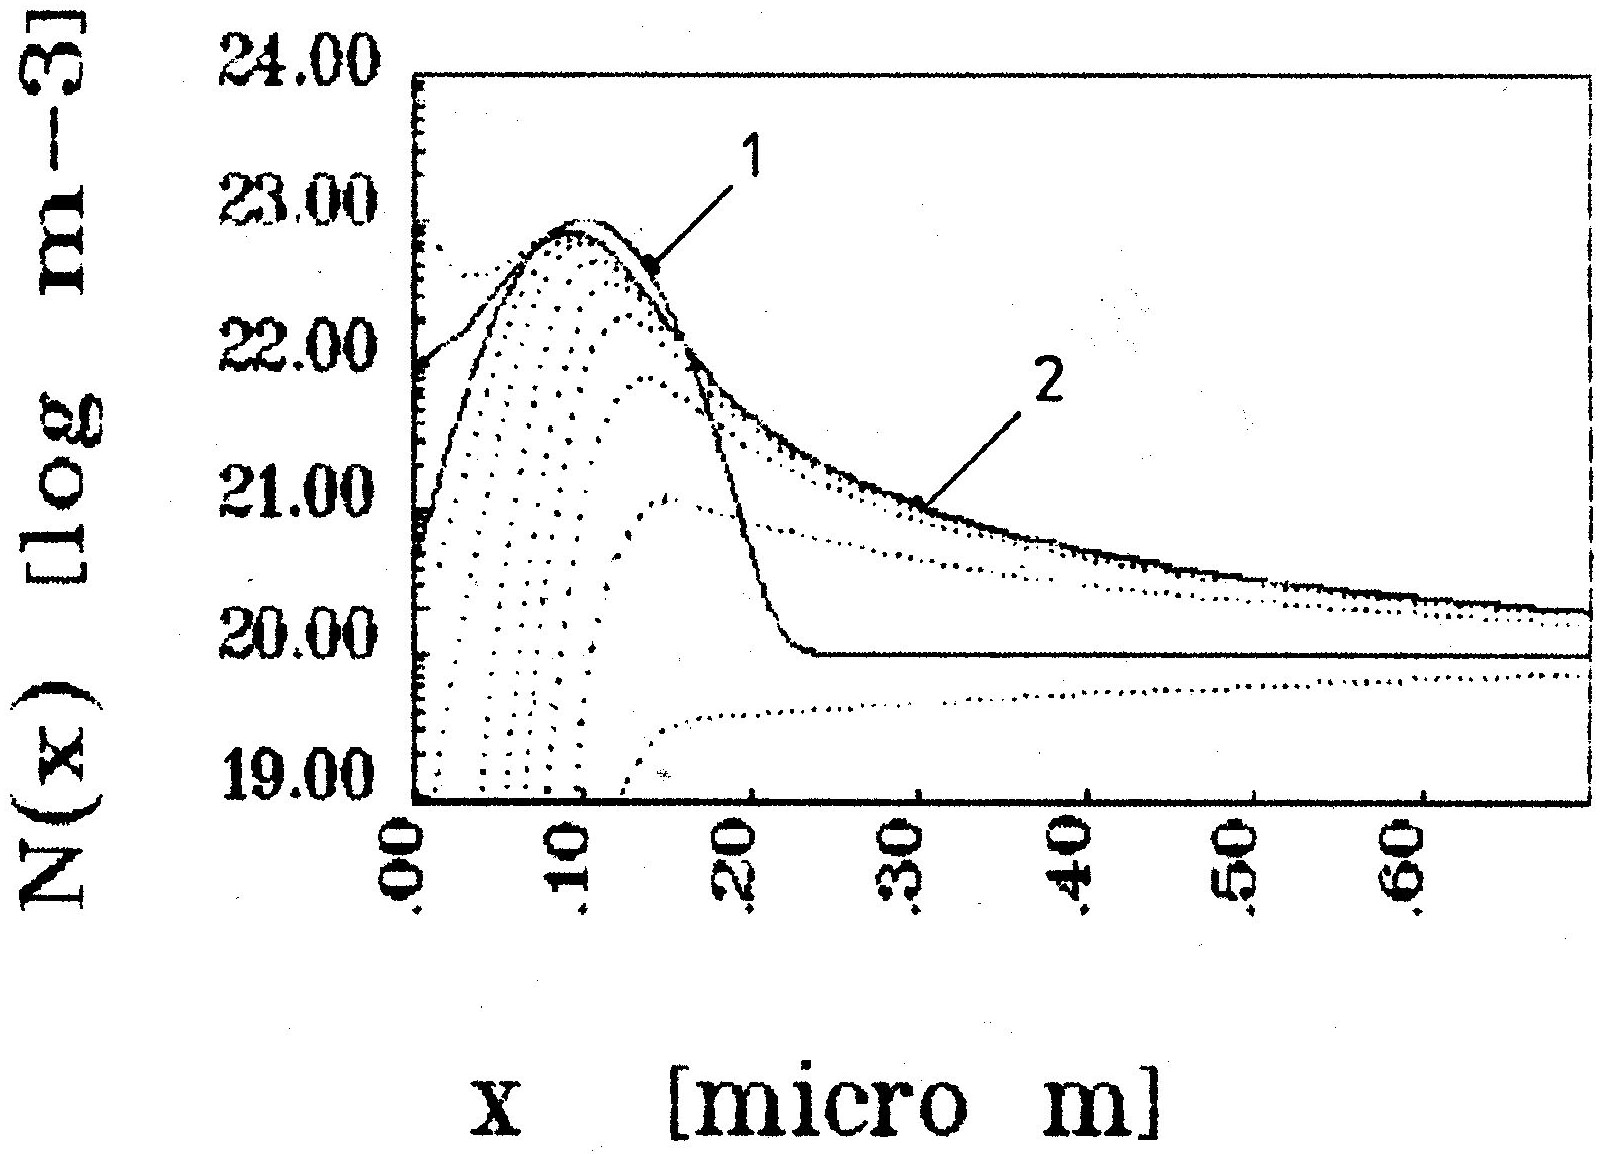
\includegraphics{Figures/fig-1-1.eps}
\captionsetup{justification=raggedright, singlelinecheck=false}
\caption[Priebeh koncentrácie prímesí v podpovrchovej oblasti
  polovodiča]{Priebeh koncentrácie prímesí v podpovrchovej oblasti
  polovodiča simulovaný Gaussovským rozložením \cite{1.11} s
  následovnými parametrami $R_p=0.1 \mu{m}$; $\Delta{R_p}=0.03
  \mu{m}$; $N_{max}=10^{23} m^{-3}$; $N_{bulk}=10^{20} m^{-3}$
  (označený plnou čiarou 1). Priebeh majoritných nosičov náboja pre
  $V_g=0$ (označený plnou čiarou 2). Bodkovanými čiarami sú znázornené
  priebehy koncentrácií majoritných nosičov pre napätia hradla rôzne
  od nuly. Stav termodynamickej rovnováhy medzi rozložením prímesí a
  nosičov náboja je popísaný v dodatku \ref{app:AppendixD}.}
\label{fig:1.1}
\end{figure}

\par Na obrázku \ref{fig:1.1} je znázornený priebeh koncentrácie
prímesí v polovodiči (simulovaný Gaussovským priebehom) a priebehy
majoritných nosičov náboja pre stav štruktúry meniaci sa od obohatenia
do inverzie, znázorňujúce dej ochudobňovania podpovrchovej oblasti
polovodiča. Tu vidieť, že priebeh koncentrácie majoritných nosičov v
implantovanej oblasti nadobúda maximum a potom klesá ku koncentrácii
substrátu, ktorú dosiahne v bode nulového elektrického potenciálu.
Zároveň je zrejmý rozdiel medzi priebehom koncentrácie prímesí a
priebehom koncentrácie majoritných nosičov náboja v stave
termodynamickej rovnováhy pre nulové napätie hradla, ktorý vzniká v
dôsledku difúzie majoritných nosičov náboja.

\begin{figure}[h!]\centering
%\framebox[10cm]{\rule{0cm}{3cm}}
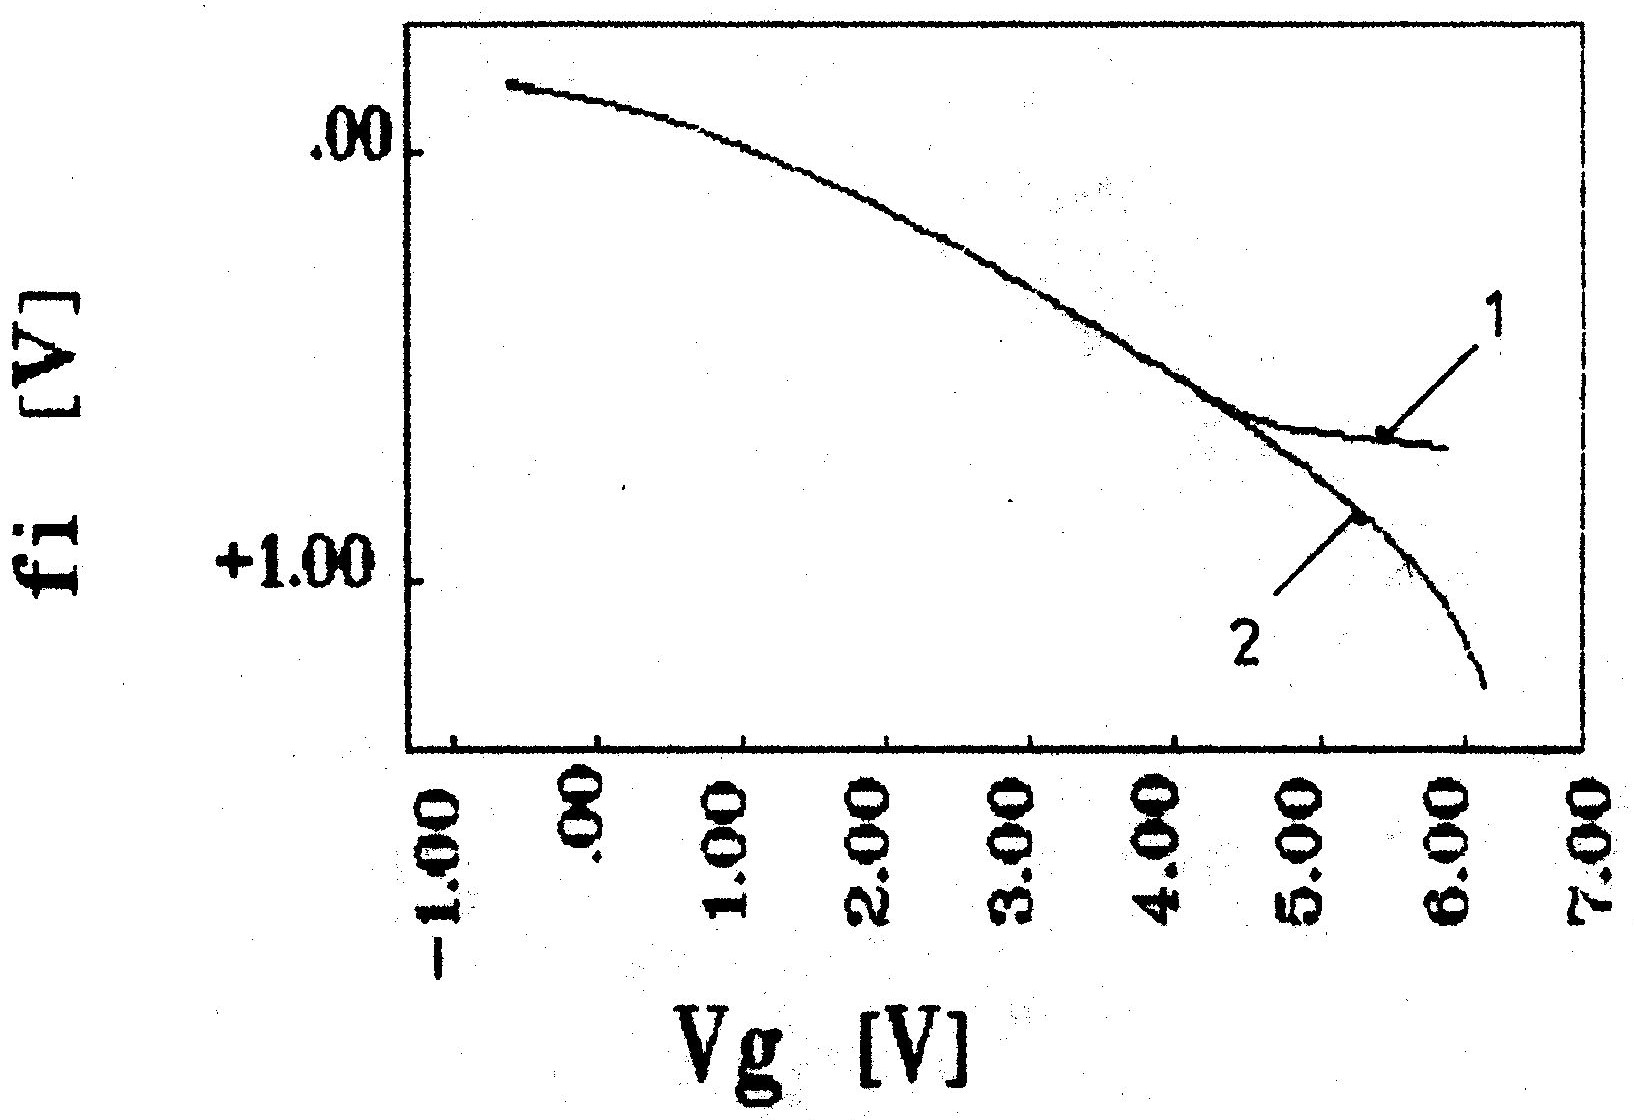
\includegraphics{Figures/fig-1-2.eps}
\captionsetup{justification=raggedright, singlelinecheck=false}
\caption[Priebeh povrchového potenciálu $\varphi_s(V_g)$ ako funkcie
  napätia hradla]{Priebeh povrchového potenciálu $\varphi_s(V_g)$ ako
  funkcie napätia hradla pre nízkofrekvenčné (LF) a vysokofrekvenčné
  (HF) meranie (označený 1) a pre meranie v stave hlbokého
  ochudobnenia (označený 2).}
\label{fig:1.2}
\end{figure}

\par Na obrázku \ref{fig:1.2} sú znázornené priebehy povrchového
potenciálu pre rôzne režimy merania štruktúry MOS. V oblasti
obohatenia a ochudobnenia sú obidva priebehy rovnaké. Od počiatku
inverzie sa povrchový potenciál pre LF a HF meranie ustaľuje v
dôsledku vytvárania inverznej vrstvy.  Krivka hlbokého ochudobnenia
ďalej klesá. Tento stav sa v reálnej štruktúre ukončí elektrickým
prierazom.

\par Na obrázku \ref{fig:1.3} sú znázornené kapacitne-napäťové
závislosti štruktúry MOS. Všetky tri krivky majú spoločný priebeh v
oblasti obohatenia a ochudobnenia (spoločný priebeh majú aj krivky
povrchového potenciálu). V tejto časti klesá kapacita pomaly, pretože
oblasť priestorového náboja sa rozpína cez oblasť s vysokou
koncentráciou prímesí (obr.1.1). Od počiatku inverzie sa krivky
rozdeľujú. Nízkofrekvenčná krivka, ktorá zaznamenáva inverznú vrstvu,
stúpa až ku kapacite oxidu. Vysokofrekvenčná krivka nezaznamenáva
inverznú vrstvu, pretože minoritné nosiče nestačia sledovať
vysokofrekvenčný merací signál, avšak kapacita už ďalej neklesá,
pretože so zvyšovaním napätia hradla sa zvyšuje prevážne koncentrácia
minoritných nosičov v inverznej vrstve a oblasť priestorového náboja
sa ďalej nerozpína.

\begin{figure}[h!]\centering
%\framebox[10cm]{\rule{0cm}{3cm}}
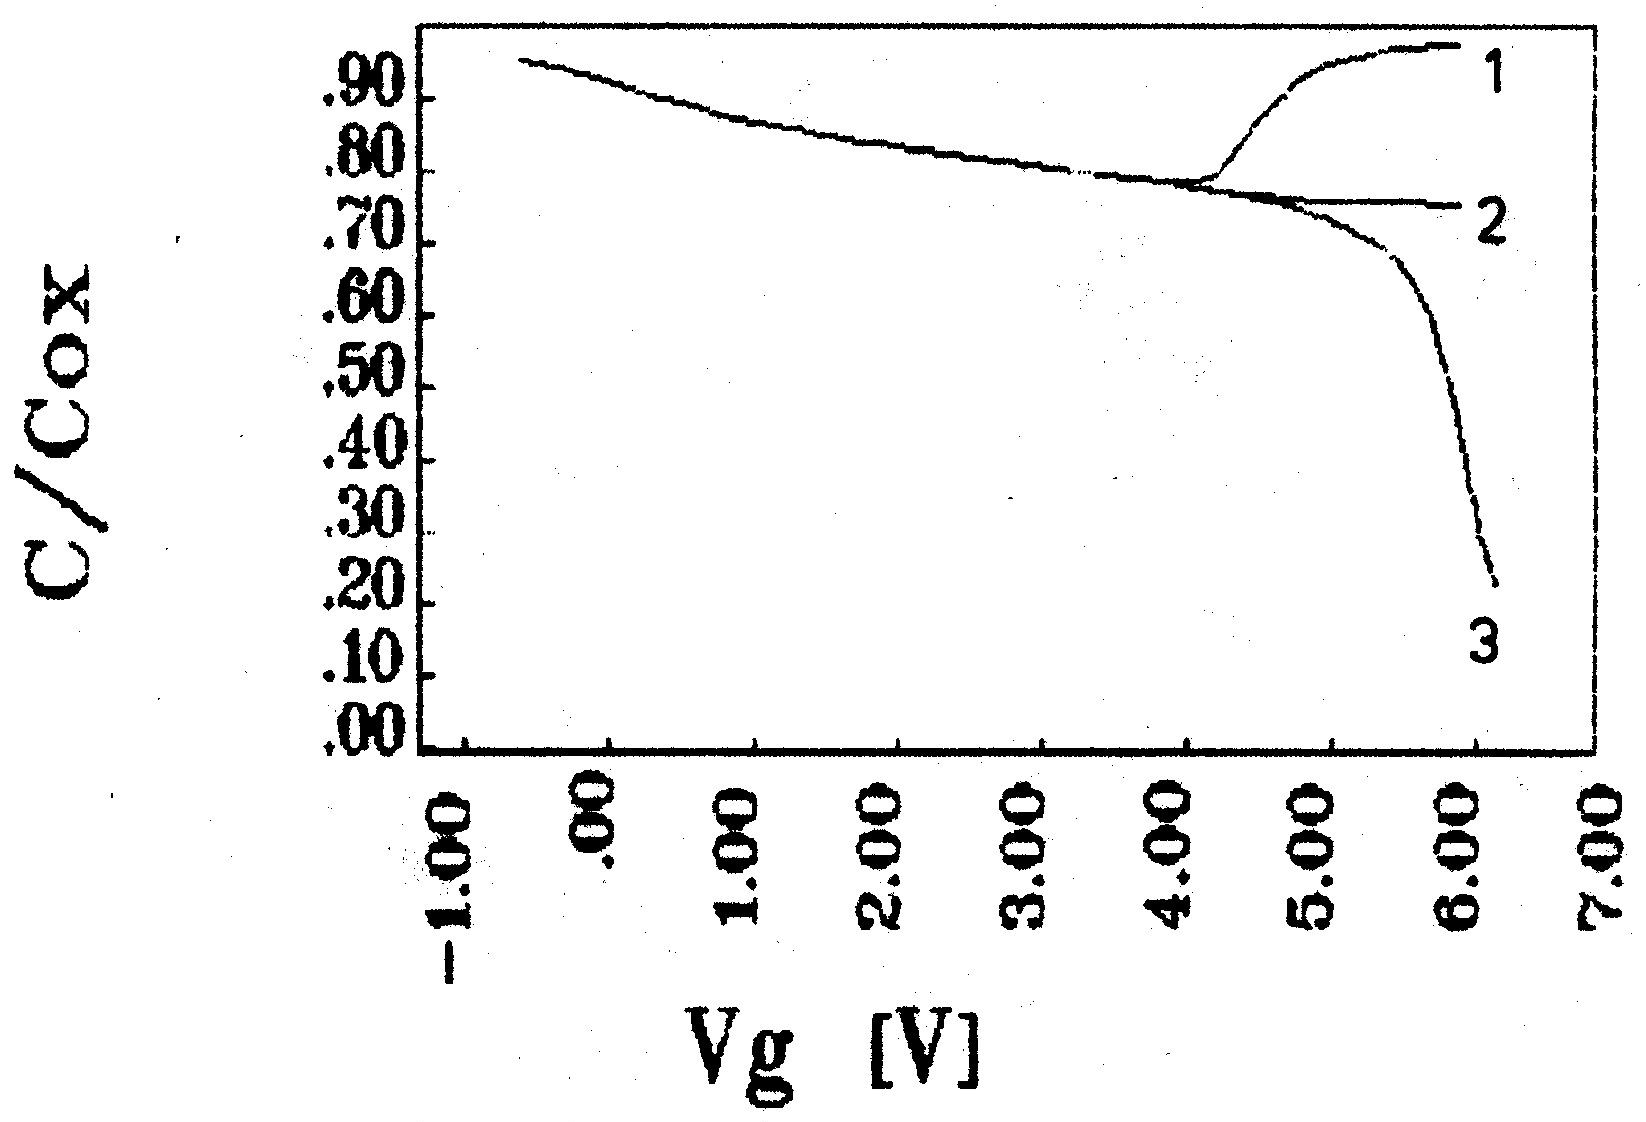
\includegraphics{Figures/fig-1-3.eps}
\captionsetup{justification=raggedright, singlelinecheck=false}
\caption[Priebeh kapacity štruktúry MOS v závislosti od napätia
  hradla]{Priebeh kapacity štruktúry MOS v závislosti od napätia
  hradla pre nízkofrekvenčné meranie (označené 1), vysokofrekvenčné
  meranie (označené 2) a meranie v stave hlbokého ochudobnenia
  (označené 3).}
\label{fig:1.3}
\end{figure}

\par V stave hlbokého ochudobnenia sa nevytvára inverzná vrstva a so
zvyšovaním napätia hradla sa oblasť priestorového náboja naďalej
rozpína a kapacita klesá. Z obrázku \ref{fig:1.3} je vidieť, že po
prekonaní oblasti s vysokou koncentráciou prímesí krivka hlbokého
ochudobnenia začína klesať rýchlejšie.

\section{Reálna štruktúra MOS.}  Odlišnosť ideálnej a reálnej
štruktúry MOS bola obsažne spracovaná v práci [1.12] a tu uvedieme len
prehľad tejto problematiky. Elektrické vlastnosti reálnej štruktúry
MOS sa líšia od ideálneho modelu hlavne vplyvom poruchových nábojov v
oxidovej vrstve a na jej rozhraní s polovodičom a kovom, ktoré možno
rozdeliť do nasledovných skupín:

\begin{itemize}
\item náboj pohyblivých iónov vo vrstve oxidu - $Q_{m}$
\item náboj ionizovaných pascí v oxide - $Q_{ox}$
\item fixný náboj na rozhraní $Si-SiO_2$ , spôsobený nestechiometrickým
  zložením v oblasti fázového prechodu - $Q_f$
\item náboj pascí na rozhraní $Si-SiO_2$  - $Q_{it}$
\end{itemize}

\par Zároveň na elektrické vlastnosti štruktúry MOS vplýva aj rozdiel
výstupných potenciálov elektrónov z kovu a polovodiča, $\varphi_{ms}\neq{0}$.
Okrem uvedených poruchových nábojov na elektrické vlastnosti štruktúry
MOS vplývajú aj geometrické nedokonalosti štruktúry, ako aj zmena
hrúbky izolačnej vrstvy a nerovinnosť plochy rozhrania $Si-SiO_2$ . Pri
prechode k veľmi veľkej integrácii vznikla potreba zaoberať sa aj
mikrodefektami v objeme kremíka, ktoré predstavujú poruchy
kryštalickej mriežky pri výrobe monokryštálu, jeho primárnom
spracovaní do formy kremíkového plátku a v priebehu technologického
spracovania súčiastky. Ak sa uvedené defekty nachádzajú vo funkčnej
oblasti súčiastky, majú nepriaznivé účinky na elektrické parametre,
avšak v objeme polovodiča mikrodefekty vhodných veľkostí spôsobujú
getračné efekty, čo sa často využíva na tvorbu tzv. denudovanej zóny.
Zámerným vytváraním mikrodefektov v objeme polovodiča pomocou
implantácie uhlíka a následným tepelným spracovaním možno napríklad
podstatne zvýšiť dobu života minoritných nosičov náboja [1.13]. V
práci [1.14] autori zreteľne zobrazili pomocou laserovej
rastrovacej tomografie denudovanú zónu pri povrchu kremíka, vytvorenú
getračnými efektami mikroprecipitátov $SiO_x$ . Zároveň je z obrázkov
vidieť mikroprecipitáty v objeme polovodiča, vytvorené pomocou kyslíka
a patričného tepelného spracovania.

\begin{thebibliography}{}
\bibitem[1.1]{1.1} Csabay O. et al: Výskum štruktúr MIS a
  pasivácie. Záverečná správa štátnej výskumnej úlohy III-4-3/2. EF
  SVŠT, Bratislava 1980.
\bibitem[1.2]{1.2} Csabay O. et al: Výskum elektrofyzikálnych
  vlastností mikroelektronických unipolárnych štruktúr. Záverečná
  správa štátnej výskumnej úlohy III-6-1/13. EF SVŠT, Bratislava 1985.
\bibitem[1.3]{1.3} Csabay O., Botka V. et al: Elektrofyzikálne
  vlastnosti mikroelektronických štruktúr. Priebežná správa Štátnej
  výskumnej úlohy III-7-2/04. Katedra mikroelektroniky EF SVŠT,
  Bratislava 1988.
\bibitem[1.4]{1.4} Csabay O., Botka V. et al: Elektrofyzikálne
  vlastnosti mikroelektronických štruktúr. Záverečná správa Štátnej
  výskumnej úlohy III-7-2/04, Katedra mikroelektroniky EF SVŠT,
  Bratislava 1990.
\bibitem[1.5]{1.5} Žiska M.: Kandidátska dizertačná práca. Katedra
  mikroelektroniky EF SVŠT, Bratislava 1985.
\bibitem[1.6]{1.6} Harmatha L.: Výskum vlastností štruktúry MIS v
  nerovnovážnom stave kapacitnou metódou. Kandidátska dizertačná
  práca. Katedra mikroelektroniky EF SVŠT, Bratislava 1983.
\bibitem[1.7]{1.7} Valehrachová D.: Kandidátska dizertačná
  práca. Katedra mikroelektroniky EF SVŠT, Bratislava
\bibitem[1.8]{1.8} Kinder R.: Príspevok ku skúmaniu koncentračných
  profilov implantovaných vrstiev. Kandidátska dizertačná práca. EF
  SVŠT Bratislava 1984.
\bibitem[1.9]{1.9}
El- Sissi H., Cobbold R.S.C.: Electronic Letters 25 (1973) s.594.
\bibitem[1.10]{1.10} Klopfenstein R. W., Wu Chung P.: IEEE Trans. on
  electron. devices ED-22 (1975) s.329.
\bibitem[1.11]{1.11}
Ryssel H., Ruge I.: Ionenimplantation. Stuttgart 1978
\bibitem[1.12]{1.12} Csabay O.: Niektoré technologické a fyzikálne
  problémy štruktúr MIS. Doktorská dizertačná práca. Katedra
  mikroelektroniky, EF SVŠT, Bratislava 1986.
\bibitem[1.13]{1.13}
Skorupa W., Kogler R. : Electronics Letters Vol.25 (1989) s.1898.
\bibitem[1.14]{1.14}
Gall P. at al. : Electronics Letters Vol.25 (1989) s.429
\end{thebibliography}

% Chapter 2
\chapter{Ciele dizertačnej práce.}\label{Chapter2}
\lhead{Kapitola 2. \emph{Ciele dizertačnej práce}}

% - - - - - - - - - - - - - - - - - - - - - - - - - - - - - - - - - - -
\begin{enumerate}
\item Vybudovanie automatizovaného experimentálneho pracoviska pre
  analýzu elektrofyzikálnych vlastností štruktúr MOS s nehomogénnym
  rozložením dotujúcich prímesí v substráte, s možnosťou sledovať
  plošné rozloženie skúmaných parametrov na kremíkovom substráte.
  Súčasťou pracoviska sú vysokofrekvenčná C-V metóda (vrátane
  ochudobnenej C-V metódy), nízkofrekvenčná C-V metóda, metóda
  konštantnej šírky OPN (CCT) a Q-C metóda.
\item Metódy uvedené v bode 1\@. automatizovať s využitím riadiaceho
  počítača PC AT pod operačným systémom MS DOS\@. Pre realizáciu metód
  využiť interfejs GPIB PCIIA, meracie prístroje HP4280a, Keithley 642
  a hrotové krokovacie zariadenie Zond A5.
\item Realizované metódy použiť pre určenie hĺbkových koncentračných
  profilov implantovaných prímesí, hrúbky oxidovej vrstvy, napätia
  vyrovnaných pásov, hustoty pascí rozhrania $Si-SiO_2$ a hĺbkového
  profilu generačného času života minoritných nosičov náboja.
  Analyzovať problémy vznikajúce pri určovaní parametrov štruktúr MOS
  v spojení s nehomogénnou dotáciou substrátu.
\item Zistiť hĺbkové koncentračné profily aktívnych prímesí a ich
  rozloženia na kremíkovom substráte pre rôzne dávky implantácie v
  rozsahu od $0.6\times{10}^{15}$ do
  $60.0\times{10}^{15}{m}^{-2}$. Zistiť ako vplýva implantačná dávka
  na vlastnosti rozhrania $Si-SiO_2$ a hĺbkový profil času života
  minoritných nosičov náboja.  Navrhnúť metodiku pre identifikáciu
  množstva implantovaných iónov v polovodičovom substráte pomocou
  kapacitnej metódy.
\end{enumerate}

% Chapter 3

\chapter{Použité metódy merania štruktúry MOS.}\label{Chapter3}
\lhead{Kapitola 3. \emph{Použité metódy merania štruktúry MOS}}
%- - - - - - - - - - - - - - - - - - - - - - - - - - - - - - - - - - -

Kapacitne-napäťové (C-V) metódy, ktorými sa v tejto práci budeme
zaoberať, poskytujú komplexné informácie o elektro-fyzikálnych
parametroch štruktúry MOS\@. Pre určenie niektorých parametrov
postačuje vyhodnotenie dát nameraných pomocou jednej metódy, no vo
väčšine prípadov kombináciou viacerých metód možno získať presnejšie
výsledky.  V predchádzajúcej kapitole sme na príklade výpočtu C-V
závislosti ideálnej štruktúry MOS demonštrovali rozdiely medzi
napäťovými závislosťami kapacity štruktúry MOS, meranými rozličnými
metódami:

\begin{itemize}
\item nízkofrekvenčnou (prípadne kvázistatickou) C-V metódou
\item rovnovážnou vysokofrekvenčnou C-V metódou
\item nerovnovážnou vysokofrekvenčnou C-V metódou.
\end{itemize}

Okrem uvedených metód sme v dizertačnej práci použili Q-C metódu,
ktorá kombinuje vlastnosti vysokofrekvenčnej a nízkofrekvenčnej C-V
metódy. Určenie tých istých C-V závislostí pomocou rôznych metód
zároveň predstavuje určitý druh kontroly presnosti merania.  To je
výhodné hlavne v prípadoch, kedy určenie absolútnej chyby merania
predstavuje komplexný problém. Pre meranie generačného času života
minoritných nosičov náboja sme použili metódu konštantnej šírky
OPN~\cite{3.1}, ktorej výhodou oproti klasickej Zerbstovej C-t
metóde~\cite{3.2} je väčšia rýchlosť merania. Modifikácia metódy
konštantnej šírky OPN~\cite{3.3} zároveň eliminuje vplyv bočnej
injekcie minoritných nosičov náboja do OPN zo substrátu.

Výhodou uvedených metód je, že nie sú deštruktívne, čo ich v spojení s
ich rýchlosťou predurčuje pre rutinné použitie v priemysle.  V
laboratórnych podmienkach je vhodné tieto metódy overiť pomocou
ďalších metód, ktoré možno považovať za doplnkové. Tak je tomu pri
meraní koncentračného profilu prímesí, napríklad metódou rozptylového
odporu, elektrochemickou kapacitnou metódou, prípadne SIMS\@. Vhodné
je aj overenie koncentračného profilu pomocou simulácie
technologického procesu. Pri skúmaní energetických stavov
nachádzajúcich sa v zakázanom pásme polovodiča, kvalitné informácie
poskytuje metóda DLTS\@.

Uvedené C-V metódy predstavujú podmnožinu širokej oblasti diagnostiky
štruktúr MOS pomocou kapacitných meraní.  Následujúca schéma
znázorňuje ich vzťah ku skúmaným parametrom, ktoré boli predmetom
tejto práce a zároveň poukazuje na okruhy problémov, ktoré bolo
potrebné riešiť.

\begin{diagram}
  \centering
  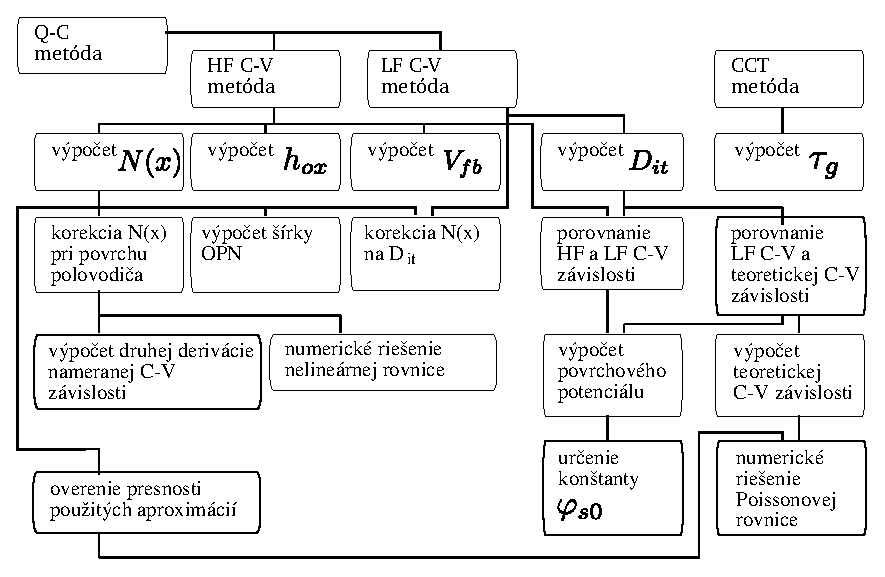
\includegraphics[width=\textwidth,height=\textheight,scale=0.7,keepaspectratio]{Figures/diagram-1.EPS}\label{diagram:1}
\end{diagram}

\section{Vysokofrekvenčná C-V metóda.}\label{sec:3.1}

Pri meraní vysokofrekvenčnou kapacitnou metódou je MOS štruktúra
jednosmerným hradlovým napätím privedená do požadovaného stavu a jej
kapacita sa určí z prúdovej odozvy na vysokofrekvenčný signál malej
amplitúdy, ktorý je nasuperponovaný na jednosmerné hradlové
napätie. Meraním fázového posuvu medzi vysokofrekvenčným napäťovým
signálom a prúdom možno okrem kapacity zároveň vyhodnotiť aj vodivosť
štruktúry. Veľkosť frekvencie meracieho signálu je daná kompromisom
medzi požiadavkou čo najvyššej frekvencie zo strany ovplyvnenia
merania rýchlymi pascami rozhrania $Si-SiO_2$ a technickými možnosťami
štandardných meracích prístrojov.  V našom experimente sme použili
prístroj HP4280a, ktorého merací signál má pevne stanovenú frekvenciu
1 MHz a veľkosť amplitúdy meracieho signálu možno voliť 10 mV, alebo
30 mV.  Spomenutý prístroj možno riadiť pomocou zbernice IMS-2. Treba
uviesť, že prístroj v spojení s riadiacim počítacom PC AT je schopný v
blokovom prenose zmerať a v binárnom formáte preniesť do riadiaceho
počítača 680 bodov (čo je limit pre blokový prenos) C-V a G-V
závislosti za 25 sekúnd.  Uvedený časový údaj uvádzame na základe
vykonaných vlastných experimentov.

\section{Kvázistatická C-V metóda.}\label{sec:3.2}

Pri meraní kvázistatickou kapacitnou metódou je MOS štruktúra nabíjaná
pomalým, v čase narastajúcim hradlovým napätím. Kapacita MOS štruktúry
je určená ako závislosť nabíjacieho prúdu a rýchlosti nárastu
hradlového napätia.  Z uvedeného vyplýva, že na realizáciu metódy je
potrebný zdroj kontinuálne narastajúceho napätia a
ampérmeter. Rýchlosť narastania napätia musí byť dostatočne malá, aby
bola štruktúra počas merania stále v termodynamickej rovnováhe. Na
druhej strane zase so zmenšovaním rýchlosti sa zmenšuje aj prúd, ktorý
musíme merať. Pre väčšinu meraných vzoriek vyhovovala rýchlosť rádove
$10^{-2}V/s$, čo predstavuje pre kapacitu $100pF$ nabíjací prúd
$10^{-12}A$. V našom experimente sme použili na meranie prúdu
elektrometer Keithley 642, ktorý meria prúd v rozsahu od $10^{-8}A$ do
$10^{-17}A$ s rozlíšením 5 číslic na rozsah.  Treba podotknúť, že
okrem iných vynikajúcich vlastností prístroja výrobca zaručuje
efektívnu hodnotu šumu menšiu ako $8\times10^{-17}A$. Zdroj
narastajúceho napätia, ktorý bol postavený na našej katedre, umožňuje
nastavenie rýchlosti nárastu napätia v rozsahoch od $10V/s$ do
$10^{-3}V/s$ s rozlíšením 1\% rozsahu. Oba prístroje možno riadiť
pomocou zbernice IMS-2.  Hlavným zdrojom chýb pri kvázistatickej
metóde je nepresnosť určenia rýchlosti nárastu napätia
hradla~\cite{1.5}. Pred každým meraním je potrebné presne zmerať
rýchlosť nárastu napätia, ktorá sa potom použije pri výpočte
kapacity. Rýchlosť nárastu napätia pre zvolený rozsah určujeme v našom
prípade z podielu zmeny napätia a času za 10 s.  Uvedená hodnota má
potom význam strednej hodnoty a jej použitie pri výpočte predpokladá
lineárny nárast napätia, ktorý sme experimentálne overili pre
reprezentatívnu vzorku rozsahov nárastu napätia v čase.

\section{Q-C metóda.}\label{sec:3.3}

Q-C metóda~\cite{3.4} predstavuje kombináciu vysokofrekvenčnej C-V
metódy a nábojovej Q-V metódy~\cite{3.5}. Jej princíp je následovný. Do
série s kondenzátorom tvoreným štruktúrou MOS je zapojená napäťovo
nezávislá kapacita, ktorú označíme $C_i$. Na sériovo-paralelné
zapojenie kondenzátorov, ktoré je znázornené na obrázku~\ref{fig:3.1},
pripojíme jednosmerné napätie $V_a$ a meriame napätie $V_i$ v
spoločnom bode zapojenia kondenzátorov, ktoré predstavujú kapacitný
delič. Kondenzátory označené $C_w$ a $C_x$ znázorňujú parazitné
kapacity. $C_w$ je kapacita medzi stolíkom a zdvihnutým hrotom sondy a
$C_x$ je kapacita spoločného bodu zapojenia kondenzátorov voči
zemi. Zároveň s meraním napätia $V_i$ zmeriame aj kapacitu $C_m$ a
vodivosť $G_m$ pomocou vysokofrekvenčného signálu nasuperponovaného na
napätí $V_a$.

\begin{figure}[h!]\centering
  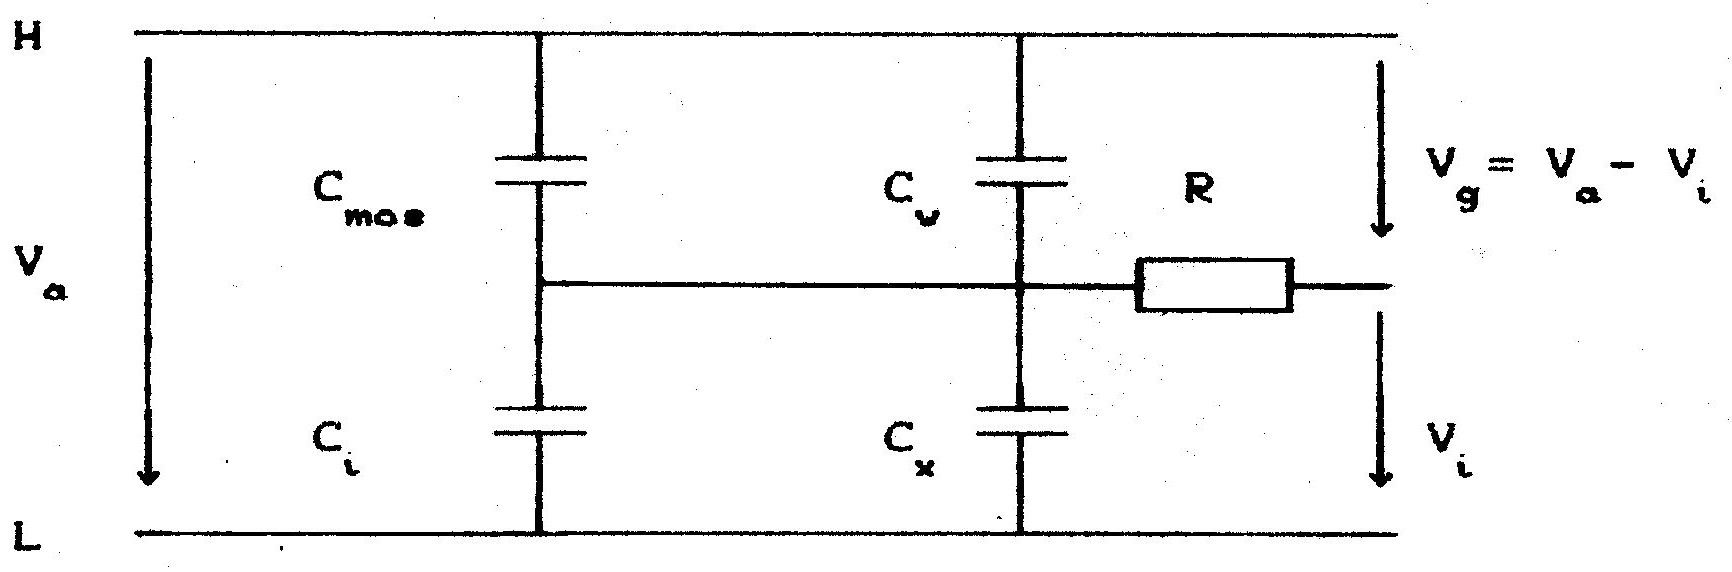
\includegraphics{Figures/fig-3-1.eps}% chktex-file 8
  \caption[Schematické znázornenie zapojenia kondenzátorov Q-C 
metódy]{Schematické znázornenie zapojenia kondenzátorov Q-C 
metódy}\label{fig:3.1}
\end{figure}

Medzi spoločný bod zapojenia kondenzátorov a vstup voltmetra je
pripojený odpor, ktorý spolu s kapacitou prívodných vodičov voltmetra
a vstupnou kapacitou voltmetra tvorí dolnopriepustný filter,
spôsobujúci, že merané napätie nie je ovplyvnené vysokofrekvenčným
signálom. Z uvedeného zároveň vyplýva, že veľkosť kapacity medzi
spoločným bodom zapojenia a bodom L sa bude líšiť pre jednosmerné a
vysokofrekvenčné meranie. Označme preto kapacitu $C_i$ pre jednosmerné
meranie $C_{iLF}$ a pre vysokofrekvenčné meranie $C_{iHF}$.  Spomenutý
odpor spolu so vstupným odporom voltmetra tvorí napäťový delič.  Aby
tým nebolo ovplyvnené meranie napätia, treba použiť voltmeter s
vysokým vstupným odporom.  Tu treba spomenúť vhodnosť použitia
elektromeru Keithley 642, ktorého vstupný odpor v režime merania
napätia je približne $10^{16} \Omega$ a jeho parazitná vstupná
kapacita sú $2 pF$. Detailný popis zapojenia Q-C metódy, eliminácia
parazitných kapacít, prípadne metodika ich merania je popísaná v
dodatku~\ref{app:AppendixE}. Ak poznáme kapacitu oxidovej vrstvy
štruktúry MOS $C_{ox}$ a veľkosť kapacity $C_{iLF}$, môžeme vypočítať
hodnotu povrchového potenciálu $\varphi_s$ z nasledovného vzťahu,
odvodeného v dodatku~\ref{app:AppendixF}.

\begin{equation}
  \varphi_s = \varphi_{s0} + V_g ( 1 + \frac{C_w}{C_{ox}}) - V_i \frac{C_{iLF}+C_x}{C_{ox}}
  \label{eq:3.1}
\end{equation}

Zároveň môžeme určiť nízkofrekvenčnú kapacitu štruktúry MOS

\begin{equation}
  C^{LF}_{mos} = C_{ox} (1 - \frac{d\varphi_s}{dV_g})
  \label{eq:3.2}
\end{equation}

Poruchové náboje nachádzajúce sa v meranej štruktúre MOS spôsobujú, že
povrchový potenciál polovodiča nadobúda hodnotu $\varphi_{s0}$ aj pri
nulovom napätí hradla. Veľkosť tejto konštanty možno určiť z
porovnania nameranej a teoretickej závislosti povrchového potenciálu
od šírky OPN $\varphi(x)$.  Metóda určenia $\varphi_{s0}$ je popísaná
v dodatku~\ref{app:AppendixG}. Tu možno poznamenať, že pre výpočet
$C^{LF}_{mos}$ hodnotu tejto konštanty nepotrebujeme, ako je zrejmé zo
vzťahov~\ref{eq:3.1} a~\ref{eq:3.2}.

Z nameraných hodnôt $C_m$ a $G_m$ môžeme určiť vysokofrekvenčnú
kapacitu štruktúry MOS pomocou nasledovných vzťahov.  Najprv
vypočítame odpovedajúci odpor $R_m$ a reaktanciu $X_m$

\begin{subequations}\label{eq:3.3}
  \begin{align}
    R_m &= \frac{G_m}{G^2_m + {(\omega C_m)}^2}\label{eq:3.3a}\\[0.3cm]
    X_m &= \frac{\omega C_m}{G^2_m + {(\omega C_m)}^2}\label{eq:3.3b}\\[0.3cm]
    \intertext{,ktoré použijeme vo vzťahu}
    C^{HF}_{mos} &= - \cfrac{R^2_m + {(X_m + \frac{1}{\omega C_{iHF}} + \omega C_w D^2)}^2}{\omega D^2{(X_m + \frac{1}{\omega C_{iHF}} + \omega C_{w} D^2)}^2}\label{eq:3.3c}\\[0.3cm]
    \intertext{,kde}
    D^2 &= R^2_m + {(X_m + \frac{1}{\omega C_{iHF}})}^2\label{eq:3.3d}
  \end{align}
\end{subequations}

Podrobný popis a odvodenie uvedených vzťahov sú popísané v
dodatku~\ref{app:AppendixE}. Q-C metóda poskytuje celý rad výhod.
Umožňuje simultánne meranie vysokofrekvenčnej a nízkofrekvenčnej C-V
závislosti, čo zaručuje rovnaké podmienky merania pre obe závislosti a
vylučuje možnosť ich vzájomného napäťového posuvu, ktorý sa môže
objaviť ak by boli závislosti snímané sekvenčne. Zároveň meranie
nízkofrekvenčnej C-V závislosti je statické a nie je závisle od
dynamiky hradlového napätia.

Pre určenie koncentračného profilu prímesí v podpovrchovej oblasti
polovodiča je výhodné poznať priebeh povrchového potenciálu, čo
umožňuje výpočet nezaťažený pascami rozhrania $Si-SiO_2$. Uvedené
výhody sú vykompenzované náročnosťou metódy na použité prístroje.
Kritickým bodom realizácie metódy je odizolovanie spoločného bodu
zapojenia kondenzátorov. Pripojené napätie $V_a$ sa musí rozložiť na
kondenzátoroch podľa ich kapacít a nie podľa ich zvodových odporov.
To vyžaduje použitie kvalitného kondenzátora $C_i$ a usporiadanie
rozloženia jednotlivých komponentov metódy tak, aby bol zvodový prúd
zo spoločného bodu na zem čo najmenší. Tým sú z použitia Q-C metódy
vylúčené štruktúry MOS, ktoré majú veľké zvodové prúdy spôsobené
nedokonalosťou oxidovej vrstvy. Pre meranie v stave termodynamickej
rovnováhy, ako uvádzajú autori metódy~\cite{3.7}, je potrebné aby sa
napätie $V_i$ nemenilo najmenej počas 10 sekúnd o veľkosť rádove
$10^{-3}V$. Pre účely určenia koncentračného profilu môžeme merať
nerovnovážnu C-V závislosť, pri ktorej sa zvodové prúdy zo spoločného
bodu na zem neprejavia v takej miere, pretože merané napätie je
odčítavané okamžite po priložení napätia. Na obrázku~\ref{fig:3.2} sú
znázornené normované priebehy HF C-V závislosti štruktúry MOS a
priebehu povrchového potenciálu od napätia hradla určené pomocou Q-C
metódy pre meranie v stave termodynamickej rovnováhy a v stave
hlbokého ochudobnenia. Použité prístroje v implementácii metódy na
našom oddelení~\cite{3.8,3.9} možno riadiť pomocou zbernice IMS-2 a
namerané hodnoty napätí $V_a$, $V_i$, kapacity $C_m$ a vodivosti $G_m$
uložiť do diskového súboru pre ďalšie spracovanie.

\begin{figure}[h!]\centering
  % GNUPLOT: LaTeX picture with Postscript
\begingroup
  \makeatletter
  \providecommand\color[2][]{%
    \GenericError{(gnuplot) \space\space\space\@spaces}{%
      Package color not loaded in conjunction with
      terminal option `colourtext'%
    }{See the gnuplot documentation for explanation.%
    }{Either use 'blacktext' in gnuplot or load the package
      color.sty in LaTeX.}%
    \renewcommand\color[2][]{}%
  }%
  \providecommand\includegraphics[2][]{%
    \GenericError{(gnuplot) \space\space\space\@spaces}{%
      Package graphicx or graphics not loaded%
    }{See the gnuplot documentation for explanation.%
    }{The gnuplot epslatex terminal needs graphicx.sty or graphics.sty.}%
    \renewcommand\includegraphics[2][]{}%
  }%
  \providecommand\rotatebox[2]{#2}%
  \@ifundefined{ifGPcolor}{%
    \newif\ifGPcolor
    \GPcolortrue
  }{}%
  \@ifundefined{ifGPblacktext}{%
    \newif\ifGPblacktext
    \GPblacktexttrue
  }{}%
  % define a \g@addto@macro without @ in the name:
  \let\gplgaddtomacro\g@addto@macro
  % define empty templates for all commands taking text:
  \gdef\gplbacktext{}%
  \gdef\gplfronttext{}%
  \makeatother
  \ifGPblacktext
    % no textcolor at all
    \def\colorrgb#1{}%
    \def\colorgray#1{}%
  \else
    % gray or color?
    \ifGPcolor
      \def\colorrgb#1{\color[rgb]{#1}}%
      \def\colorgray#1{\color[gray]{#1}}%
      \expandafter\def\csname LTw\endcsname{\color{white}}%
      \expandafter\def\csname LTb\endcsname{\color{black}}%
      \expandafter\def\csname LTa\endcsname{\color{black}}%
      \expandafter\def\csname LT0\endcsname{\color[rgb]{1,0,0}}%
      \expandafter\def\csname LT1\endcsname{\color[rgb]{0,1,0}}%
      \expandafter\def\csname LT2\endcsname{\color[rgb]{0,0,1}}%
      \expandafter\def\csname LT3\endcsname{\color[rgb]{1,0,1}}%
      \expandafter\def\csname LT4\endcsname{\color[rgb]{0,1,1}}%
      \expandafter\def\csname LT5\endcsname{\color[rgb]{1,1,0}}%
      \expandafter\def\csname LT6\endcsname{\color[rgb]{0,0,0}}%
      \expandafter\def\csname LT7\endcsname{\color[rgb]{1,0.3,0}}%
      \expandafter\def\csname LT8\endcsname{\color[rgb]{0.5,0.5,0.5}}%
    \else
      % gray
      \def\colorrgb#1{\color{black}}%
      \def\colorgray#1{\color[gray]{#1}}%
      \expandafter\def\csname LTw\endcsname{\color{white}}%
      \expandafter\def\csname LTb\endcsname{\color{black}}%
      \expandafter\def\csname LTa\endcsname{\color{black}}%
      \expandafter\def\csname LT0\endcsname{\color{black}}%
      \expandafter\def\csname LT1\endcsname{\color{black}}%
      \expandafter\def\csname LT2\endcsname{\color{black}}%
      \expandafter\def\csname LT3\endcsname{\color{black}}%
      \expandafter\def\csname LT4\endcsname{\color{black}}%
      \expandafter\def\csname LT5\endcsname{\color{black}}%
      \expandafter\def\csname LT6\endcsname{\color{black}}%
      \expandafter\def\csname LT7\endcsname{\color{black}}%
      \expandafter\def\csname LT8\endcsname{\color{black}}%
    \fi
  \fi
    \setlength{\unitlength}{0.0500bp}%
    \ifx\gptboxheight\undefined%
      \newlength{\gptboxheight}%
      \newlength{\gptboxwidth}%
      \newsavebox{\gptboxtext}%
    \fi%
    \setlength{\fboxrule}{0.5pt}%
    \setlength{\fboxsep}{1pt}%
\begin{picture}(7920.00,5616.00)%
    \gplgaddtomacro\gplbacktext{%
      \csname LTb\endcsname%%
      \put(740,640){\makebox(0,0)[r]{\strut{}$0$}}%
      \put(740,1369){\makebox(0,0)[r]{\strut{}$0.2$}}%
      \put(740,2098){\makebox(0,0)[r]{\strut{}$0.4$}}%
      \put(740,2828){\makebox(0,0)[r]{\strut{}$0.6$}}%
      \put(740,3557){\makebox(0,0)[r]{\strut{}$0.8$}}%
      \put(740,4286){\makebox(0,0)[r]{\strut{}$1$}}%
      \put(740,5015){\makebox(0,0)[r]{\strut{}$1.2$}}%
      \put(860,440){\makebox(0,0){\strut{}$-2$}}%
      \put(1977,440){\makebox(0,0){\strut{}$0$}}%
      \put(3093,440){\makebox(0,0){\strut{}$2$}}%
      \put(4210,440){\makebox(0,0){\strut{}$4$}}%
      \put(5326,440){\makebox(0,0){\strut{}$6$}}%
      \put(6443,440){\makebox(0,0){\strut{}$8$}}%
      \put(7559,440){\makebox(0,0){\strut{}$10$}}%
    }%
    \gplgaddtomacro\gplfronttext{%
      \csname LTb\endcsname%%
      \put(190,2827){\rotatebox{-270}{\makebox(0,0){\strut{}${C}/{C}_{ox}$ \qquad $(1-{\varphi}/{\varphi}_{norm})$}}}%
      \put(4209,140){\makebox(0,0){\strut{}Napätie hradla ${V}_g$}}%
      \put(4209,5315){\makebox(0,0){\strut{}QC metóda}}%
      \csname LTb\endcsname%%
      \put(6339,1647){\makebox(0,0)[l]{\strut{}${C}_{mos}^{DD}$}}%
      \csname LTb\endcsname%%
      \put(6339,1165){\makebox(0,0)[l]{\strut{}${\varphi}_{s}^{DD}$}}%
      \csname LTb\endcsname%%
      \put(5985,2989){\makebox(0,0)[l]{\strut{}${C}_{mos}^{HF}$}}%
      \csname LTb\endcsname%%
      \put(5985,3447){\makebox(0,0)[l]{\strut{}${\varphi}_{s}^{HF}$}}%
    }%
    \gplbacktext
    \put(0,0){\includegraphics{/export/scratch/vbotka-thesis/Plot/Figures/fig-3-2-sk}}%
    \gplfronttext
  \end{picture}%
\endgroup

  \caption[Normované priebehy HF C-V závislosti štruktúry MOS a
    priebehu povrchového potenciálu od napätia hradla určené pomocou
    Q-C metódy pre meranie v stave termodynamickej rovnováhy a v stave
    hlbokého ochudobnenia]{Normované priebehy HF C-V závislosti
    štruktúry MOS a priebehu povrchového potenciálu od napätia hradla
    určené pomocou Q-C metódy pre meranie v stave termodynamickej
    rovnováhy a v stave hlbokého ochudobnenia. Priebehy
    $\varphi_s(V_g)$ sú zobrazené s použitím normovania $1 - {\varphi_s}/{\varphi_{norm}}$, kde
    $\varphi_{norm}=3.33V$.}\label{fig:3.2}
\end{figure}
%OBR7.BIT

Pre overenie presnosti Q-C metódy sme na tej istej štruktúre MOS
urobili samostatné vysokofrekvenčné a nízkofrekvenčné meranie a
zároveň vypočítali tie isté kapacitné závislosti z nameraných hodnôt
Q-C metódy.  Výsledné krivky sú na obrázkoch~\ref{fig:3.3} a~\ref{fig:3.4}.

Pre kvantitatívne porovnanie výsledkov znázornených na
obrázku~\ref{fig:3.3} a~\ref{fig:3.4} uvádzame v tabuľke~\ref{tab:3.1}
a~\ref{tab:3.2} číselné hodnoty normovaných kapacít $C^{HF}_{mos}$ a
$C^{LF}_{mos}$ pre metódy HF, LF a Q-C a ich rozdiel vyjadrený
relatívnou chybou. Z tabuliek vidieť rozdiel medzi jednotlivými C-V
závislosťami, čo je spôsobené jednak nepresnosťami pri určovaní
parazitných kapacít a jednak zvodovými prúdmi použitých
kondenzátorov. Autori metódy doporučujú pre elimináciu zvodových
prúdov, ktoré spôsobuje vlhkosť prostredia, použiť vzduchový
kondenzátor $C_i$ a na meranú vzorku usmerniť v priebehu merania prúd
dusíka, ktorý zabráni kondenzovaniu vodných pár z okolia.

\newpage
\begin{figure}[h!]\centering
  % GNUPLOT: LaTeX picture with Postscript
\begingroup
  \makeatletter
  \providecommand\color[2][]{%
    \GenericError{(gnuplot) \space\space\space\@spaces}{%
      Package color not loaded in conjunction with
      terminal option `colourtext'%
    }{See the gnuplot documentation for explanation.%
    }{Either use 'blacktext' in gnuplot or load the package
      color.sty in LaTeX.}%
    \renewcommand\color[2][]{}%
  }%
  \providecommand\includegraphics[2][]{%
    \GenericError{(gnuplot) \space\space\space\@spaces}{%
      Package graphicx or graphics not loaded%
    }{See the gnuplot documentation for explanation.%
    }{The gnuplot epslatex terminal needs graphicx.sty or graphics.sty.}%
    \renewcommand\includegraphics[2][]{}%
  }%
  \providecommand\rotatebox[2]{#2}%
  \@ifundefined{ifGPcolor}{%
    \newif\ifGPcolor
    \GPcolortrue
  }{}%
  \@ifundefined{ifGPblacktext}{%
    \newif\ifGPblacktext
    \GPblacktextfalse
  }{}%
  % define a \g@addto@macro without @ in the name:
  \let\gplgaddtomacro\g@addto@macro
  % define empty templates for all commands taking text:
  \gdef\gplbacktext{}%
  \gdef\gplfronttext{}%
  \makeatother
  \ifGPblacktext
    % no textcolor at all
    \def\colorrgb#1{}%
    \def\colorgray#1{}%
  \else
    % gray or color?
    \ifGPcolor
      \def\colorrgb#1{\color[rgb]{#1}}%
      \def\colorgray#1{\color[gray]{#1}}%
      \expandafter\def\csname LTw\endcsname{\color{white}}%
      \expandafter\def\csname LTb\endcsname{\color{black}}%
      \expandafter\def\csname LTa\endcsname{\color{black}}%
      \expandafter\def\csname LT0\endcsname{\color[rgb]{1,0,0}}%
      \expandafter\def\csname LT1\endcsname{\color[rgb]{0,1,0}}%
      \expandafter\def\csname LT2\endcsname{\color[rgb]{0,0,1}}%
      \expandafter\def\csname LT3\endcsname{\color[rgb]{1,0,1}}%
      \expandafter\def\csname LT4\endcsname{\color[rgb]{0,1,1}}%
      \expandafter\def\csname LT5\endcsname{\color[rgb]{1,1,0}}%
      \expandafter\def\csname LT6\endcsname{\color[rgb]{0,0,0}}%
      \expandafter\def\csname LT7\endcsname{\color[rgb]{1,0.3,0}}%
      \expandafter\def\csname LT8\endcsname{\color[rgb]{0.5,0.5,0.5}}%
    \else
      % gray
      \def\colorrgb#1{\color{black}}%
      \def\colorgray#1{\color[gray]{#1}}%
      \expandafter\def\csname LTw\endcsname{\color{white}}%
      \expandafter\def\csname LTb\endcsname{\color{black}}%
      \expandafter\def\csname LTa\endcsname{\color{black}}%
      \expandafter\def\csname LT0\endcsname{\color{black}}%
      \expandafter\def\csname LT1\endcsname{\color{black}}%
      \expandafter\def\csname LT2\endcsname{\color{black}}%
      \expandafter\def\csname LT3\endcsname{\color{black}}%
      \expandafter\def\csname LT4\endcsname{\color{black}}%
      \expandafter\def\csname LT5\endcsname{\color{black}}%
      \expandafter\def\csname LT6\endcsname{\color{black}}%
      \expandafter\def\csname LT7\endcsname{\color{black}}%
      \expandafter\def\csname LT8\endcsname{\color{black}}%
    \fi
  \fi
    \setlength{\unitlength}{0.0500bp}%
    \ifx\gptboxheight\undefined%
      \newlength{\gptboxheight}%
      \newlength{\gptboxwidth}%
      \newsavebox{\gptboxtext}%
    \fi%
    \setlength{\fboxrule}{0.5pt}%
    \setlength{\fboxsep}{1pt}%
\begin{picture}(7920.00,5616.00)%
    \gplgaddtomacro\gplbacktext{%
      \csname LTb\endcsname%%
      \put(740,640){\makebox(0,0)[r]{\strut{}$0.5$}}%
      \put(740,1369){\makebox(0,0)[r]{\strut{}$0.6$}}%
      \put(740,2098){\makebox(0,0)[r]{\strut{}$0.7$}}%
      \put(740,2827){\makebox(0,0)[r]{\strut{}$0.8$}}%
      \put(740,3557){\makebox(0,0)[r]{\strut{}$0.9$}}%
      \put(740,4286){\makebox(0,0)[r]{\strut{}$1$}}%
      \put(740,5015){\makebox(0,0)[r]{\strut{}$1.1$}}%
      \put(860,440){\makebox(0,0){\strut{}$-6$}}%
      \put(1697,440){\makebox(0,0){\strut{}$-5$}}%
      \put(2535,440){\makebox(0,0){\strut{}$-4$}}%
      \put(3372,440){\makebox(0,0){\strut{}$-3$}}%
      \put(4210,440){\makebox(0,0){\strut{}$-2$}}%
      \put(5047,440){\makebox(0,0){\strut{}$-1$}}%
      \put(5884,440){\makebox(0,0){\strut{}$0$}}%
      \put(6722,440){\makebox(0,0){\strut{}$1$}}%
      \put(7559,440){\makebox(0,0){\strut{}$2$}}%
    }%
    \gplgaddtomacro\gplfronttext{%
      \csname LTb\endcsname%%
      \put(190,2827){\rotatebox{-270}{\makebox(0,0){\strut{}${C}/{C}_{ox}$ \qquad $(1-{\varphi}/{\varphi}_{norm})$}}}%
      \put(4209,140){\makebox(0,0){\strut{}Napätie hradla ${V}_g$}}%
      \put(4209,5315){\makebox(0,0){\strut{}QC metóda}}%
      \colorrgb{0.55,0.00,0.00}%%
      \put(6656,2903){\makebox(0,0)[r]{\strut{}${\varphi}_{s}^{QC}$}}%
      \colorrgb{0.78,0.08,0.52}%%
      \put(6656,2503){\makebox(0,0)[r]{\strut{}${C}_{mos}^{QC}$}}%
      \colorrgb{1.00,0.27,0.00}%%
      \put(6656,2103){\makebox(0,0)[r]{\strut{}${C}_{mos}^{QC}$}}%
      \colorrgb{0.00,0.55,0.55}%%
      \put(6656,1703){\makebox(0,0)[r]{\strut{}${C}_{mos}^{HF}$}}%
      \colorrgb{0.00,0.00,1.00}%%
      \put(6656,1303){\makebox(0,0)[r]{\strut{}${C}_{mos}^{LF}$}}%
      \colorrgb{0.44,0.50,0.56}%%
      \put(6656,903){\makebox(0,0)[r]{\strut{}${\varphi}_{s}^{DD}$}}%
    }%
    \gplbacktext
    \put(0,0){\includegraphics{/export/scratch/vbotka-thesis/Plot/Figures/fig-3-3-sk}}%
    \gplfronttext
  \end{picture}%
\endgroup

  \caption[Normované priebehy kapacity štruktúry MOS so substrátom
    typu N pre rovnovážne HF a kvázistatické meranie]{Normované
    priebehy kapacity štruktúry MOS so substrátom typu N pre
    rovnovážne HF a kvázistatické meranie. Zároveň sú znázornené tie
    isté charakteristiky získané pomocou Q-C metódy. Pre úplnosť je
    znázornená závislosť povrchového potenciálu
    ${\varphi_s(V_g)}^{QC}$ získaná pomocou Q-C metódy a závislosť
    ${\varphi_s(V_g)}^{LF}$ vypočítaná integrovaním nízkofrekvenčnej
    C-V závislosti pomocou Berglundovho integrálu.  Priebehy
    $\varphi_s(V_g)$ sú normované $1 -
    \frac{\varphi_s}{\varphi_{norm}}$, kde
    $\varphi_{norm}=-4.66V$.}\label{fig:3.3}
\end{figure}
%OBR5.BIT

\begin{table}[h!]\centering
  \begin{tabular}{c c c c c c}
    \multicolumn{3}{l}{$C^{HF}_{mos}$} & \multicolumn{3}{l}{$C^{LF}_{mos}$} \\
    HF[\%] & QC[\%] & $\Delta_r$[\%] & LF[\%] & QC[\%] & $\Delta_r$[\%] \\
    \hline% chktex-file 44
    99.67 & 98.30 & +1.37 & 97.85 & 99.14 & -1.32 \\
    98.56 & 96.69 & +1.89 & 96.59 & 97.05 & -0.47 \\
    98.56 & 96.69 & +1.89 & 96.59 & 97.05 & -0.47 \\
    95.73 & 93.89 & +1.92 & 93.93 & 94.51 & -0.61 \\
    89.89 & 87.75 & +2.39 & 88.26 & 88.57 & -0.36 \\
    82.15 & 80.17 & +2.41 & 81.43 & 81.82 & -0.47 \\
    74.83 & 73.09 & +2.33 & 73.79 & 74.57 & -1.06 \\
    69.69 & 67.81 & +2.70 & 86.08 & 86.33 & -0.29 \\
    69.10 & 67.20 & +2.74 & 97.20 & 97.73 & -0.54 \\
    68.97 & 67.08 & +2.74 & 98.27 & 98.74 & -0.48 \\
    68.91 & 67.03 & +2.72 & 98.75 & 99.38 & -0.64 \\
    68.90 & 67.01 & +2.75 & 99.04 & 98.68 & -0.36 \\
    68.90 & 67.03 & +2.70 & 99.20 & 99.87 & -0.67 \\
  \end{tabular}
  \caption[Porovnanie normovanej vysokofrekvenčnej a nízkofrekvenčnej
    kapacity štruktúry MOS (obrázok~\ref{fig:3.3}) pre metódy HF, LF a
    Q-C]{Porovnanie normovanej vysokofrekvenčnej a nízkofrekvenčnej
    kapacity štruktúry MOS (obrázok~\ref{fig:3.3}) pre metódy HF, LF a
    Q-C. Rozdiel kriviek je vyjadrený relatívnou chybou.}\label{tab:3.1}
\end{table}

\newpage
\begin{figure}[h!]\centering
  % GNUPLOT: LaTeX picture with Postscript
\begingroup
  \makeatletter
  \providecommand\color[2][]{%
    \GenericError{(gnuplot) \space\space\space\@spaces}{%
      Package color not loaded in conjunction with
      terminal option `colourtext'%
    }{See the gnuplot documentation for explanation.%
    }{Either use 'blacktext' in gnuplot or load the package
      color.sty in LaTeX.}%
    \renewcommand\color[2][]{}%
  }%
  \providecommand\includegraphics[2][]{%
    \GenericError{(gnuplot) \space\space\space\@spaces}{%
      Package graphicx or graphics not loaded%
    }{See the gnuplot documentation for explanation.%
    }{The gnuplot epslatex terminal needs graphicx.sty or graphics.sty.}%
    \renewcommand\includegraphics[2][]{}%
  }%
  \providecommand\rotatebox[2]{#2}%
  \@ifundefined{ifGPcolor}{%
    \newif\ifGPcolor
    \GPcolortrue
  }{}%
  \@ifundefined{ifGPblacktext}{%
    \newif\ifGPblacktext
    \GPblacktextfalse
  }{}%
  % define a \g@addto@macro without @ in the name:
  \let\gplgaddtomacro\g@addto@macro
  % define empty templates for all commands taking text:
  \gdef\gplbacktext{}%
  \gdef\gplfronttext{}%
  \makeatother
  \ifGPblacktext
    % no textcolor at all
    \def\colorrgb#1{}%
    \def\colorgray#1{}%
  \else
    % gray or color?
    \ifGPcolor
      \def\colorrgb#1{\color[rgb]{#1}}%
      \def\colorgray#1{\color[gray]{#1}}%
      \expandafter\def\csname LTw\endcsname{\color{white}}%
      \expandafter\def\csname LTb\endcsname{\color{black}}%
      \expandafter\def\csname LTa\endcsname{\color{black}}%
      \expandafter\def\csname LT0\endcsname{\color[rgb]{1,0,0}}%
      \expandafter\def\csname LT1\endcsname{\color[rgb]{0,1,0}}%
      \expandafter\def\csname LT2\endcsname{\color[rgb]{0,0,1}}%
      \expandafter\def\csname LT3\endcsname{\color[rgb]{1,0,1}}%
      \expandafter\def\csname LT4\endcsname{\color[rgb]{0,1,1}}%
      \expandafter\def\csname LT5\endcsname{\color[rgb]{1,1,0}}%
      \expandafter\def\csname LT6\endcsname{\color[rgb]{0,0,0}}%
      \expandafter\def\csname LT7\endcsname{\color[rgb]{1,0.3,0}}%
      \expandafter\def\csname LT8\endcsname{\color[rgb]{0.5,0.5,0.5}}%
    \else
      % gray
      \def\colorrgb#1{\color{black}}%
      \def\colorgray#1{\color[gray]{#1}}%
      \expandafter\def\csname LTw\endcsname{\color{white}}%
      \expandafter\def\csname LTb\endcsname{\color{black}}%
      \expandafter\def\csname LTa\endcsname{\color{black}}%
      \expandafter\def\csname LT0\endcsname{\color{black}}%
      \expandafter\def\csname LT1\endcsname{\color{black}}%
      \expandafter\def\csname LT2\endcsname{\color{black}}%
      \expandafter\def\csname LT3\endcsname{\color{black}}%
      \expandafter\def\csname LT4\endcsname{\color{black}}%
      \expandafter\def\csname LT5\endcsname{\color{black}}%
      \expandafter\def\csname LT6\endcsname{\color{black}}%
      \expandafter\def\csname LT7\endcsname{\color{black}}%
      \expandafter\def\csname LT8\endcsname{\color{black}}%
    \fi
  \fi
    \setlength{\unitlength}{0.0500bp}%
    \ifx\gptboxheight\undefined%
      \newlength{\gptboxheight}%
      \newlength{\gptboxwidth}%
      \newsavebox{\gptboxtext}%
    \fi%
    \setlength{\fboxrule}{0.5pt}%
    \setlength{\fboxsep}{1pt}%
\begin{picture}(7920.00,5616.00)%
    \gplgaddtomacro\gplbacktext{%
      \csname LTb\endcsname%%
      \put(740,640){\makebox(0,0)[r]{\strut{}$0.5$}}%
      \put(740,1369){\makebox(0,0)[r]{\strut{}$0.6$}}%
      \put(740,2098){\makebox(0,0)[r]{\strut{}$0.7$}}%
      \put(740,2827){\makebox(0,0)[r]{\strut{}$0.8$}}%
      \put(740,3557){\makebox(0,0)[r]{\strut{}$0.9$}}%
      \put(740,4286){\makebox(0,0)[r]{\strut{}$1$}}%
      \put(740,5015){\makebox(0,0)[r]{\strut{}$1.1$}}%
      \put(860,440){\makebox(0,0){\strut{}$-2$}}%
      \put(1697,440){\makebox(0,0){\strut{}$-1$}}%
      \put(2535,440){\makebox(0,0){\strut{}$0$}}%
      \put(3372,440){\makebox(0,0){\strut{}$1$}}%
      \put(4210,440){\makebox(0,0){\strut{}$2$}}%
      \put(5047,440){\makebox(0,0){\strut{}$3$}}%
      \put(5884,440){\makebox(0,0){\strut{}$4$}}%
      \put(6722,440){\makebox(0,0){\strut{}$5$}}%
      \put(7559,440){\makebox(0,0){\strut{}$6$}}%
    }%
    \gplgaddtomacro\gplfronttext{%
      \csname LTb\endcsname%%
      \put(190,2827){\rotatebox{-270}{\makebox(0,0){\strut{}${C}/{C}_{ox}$ \qquad $(1-{\varphi}/{\varphi}_{norm})$}}}%
      \put(4209,140){\makebox(0,0){\strut{}Napätie hradla ${V}_g$}}%
      \put(4209,5315){\makebox(0,0){\strut{}QC metóda}}%
      \colorrgb{0.55,0.00,0.00}%%
      \put(1700,2903){\makebox(0,0)[r]{\strut{}${\varphi}_{s}^{QC}$}}%
      \colorrgb{0.78,0.08,0.52}%%
      \put(1700,2503){\makebox(0,0)[r]{\strut{}${C}_{mos}^{QC}$}}%
      \colorrgb{1.00,0.27,0.00}%%
      \put(1700,2103){\makebox(0,0)[r]{\strut{}${C}_{mos}^{QC}$}}%
      \colorrgb{0.00,0.55,0.55}%%
      \put(1700,1703){\makebox(0,0)[r]{\strut{}${C}_{mos}^{HF}$}}%
      \colorrgb{0.00,0.00,1.00}%%
      \put(1700,1303){\makebox(0,0)[r]{\strut{}${C}_{mos}^{LF}$}}%
      \colorrgb{0.44,0.50,0.56}%%
      \put(1700,903){\makebox(0,0)[r]{\strut{}${\varphi}_{s}^{DD}$}}%
    }%
    \gplbacktext
    \put(0,0){\includegraphics{/export/scratch/vbotka-thesis/Plot/Figures/fig-3-4-sk}}%
    \gplfronttext
  \end{picture}%
\endgroup

  \caption[Normované priebehy kapacity štruktúry MOS so substrátom
    typu P ako funkcie napätia hradla pre rovnovážne vysokofrekvenčné
    a kvázistatické meranie]{Normované priebehy kapacity štruktúry MOS
    so substrátom typu P ako funkcie napätia hradla pre rovnovážne
    vysokofrekvenčné a kvázistatické meranie.  Zároveň sú znázornené
    tie isté charakteristiky získané pomocou Q-C metódy. Pre úplnosť
    je na obrázku znázornená závislosť povrchového potenciálu
    ${\varphi_s(V_g)}^{QC}$ získaná pomocou Q-C metódy a závislosť
    ${\varphi_s(V_g)}^{LF}$ vypočítaná integrovaním nízkofrekvenčnej
    C-V závislosti pomocou Berglundovho integrálu.  Priebehy
    $\varphi_s(V_g)$ sú zobrazené s použitím normovania $1 -
    {\varphi_s}/{\varphi_{norm}}$, kde
    $\varphi_{norm}=3.33V$.}\label{fig:3.4}
\end{figure}
%OBR6.BIT

\begin{table}[h!]\centering
  \begin{tabular}{c c c c c c}
  \multicolumn{3}{l}{$C^{HF}_{mos}$} & \multicolumn{3}{l}{$C^{LF}_{mos}$} \\
  HF[\%] & QC[\%] & $\Delta_r$[\%] & LF[\%] & QC[\%] & $\Delta_r$[\%] \\
  \hline
  96.30 & 95.71 & +0.62 & 94.80 & 94.89 & -0.09 \\
  92.88 & 92.07 & +0.87 & 91.03 & 92.83 & -1.98 \\
  87.52 & 86.48 & +1.19 & 85.97 & 87.53 & -1.81 \\
  81.39 & 80.09 & +1.60 & 79.70 & 81.20 & -1.88 \\
  75.71 & 74.55 & +1.53 & 74.24 & 76.00 & -2.37 \\
  71.17 & 69.79 & +1.98 & 69.89 & 70.65 & -1.08 \\
  67.77 & 66.41 & +2.00 & 80.77 & 83.57 & -3.47 \\
  67.14 & 65.85 & +1.93 & 94.72 & 96.93 & -2.33 \\
  66.82 & 65.73 & +1.62 & 96.77 & 98.26 & -1.53 \\
  66.65 & 65.63 & +1.52 & 97.47 & 98.06 & -0.60 \\
  66.62 & 65.59 & +1.53 & 97.94 & 99.46 & -1.56 \\
  66.58 & 65.54 & +1.56 & 98.15 & 99.39 & -1.26 \\
  \end{tabular}
  \caption[Porovnanie normovanej vysokofrekvenčnej a
  nízkofrekvenčnej kapacity štruktúry MOS (obrázok~\ref{fig:3.4}) pre
  metódy HF, LF a Q-C]{Porovnanie normovanej vysokofrekvenčnej a
  nízkofrekvenčnej kapacity štruktúry MOS (obrázok~\ref{fig:3.4}) pre
  metódy HF, LF a Q-C. Rozdiel kriviek je vyjadrený relatívnou
  chybou.}\label{tab:3.2}
\end{table}

\section{Metóda konštantnej šírky OPN a určenie generačného času života minoritných nosičov náboja.}\label{sec:3.4}

Kvalitu substrátu štruktúry MOS možno posúdiť z generačného času
života minoritných nosičov náboja, ktorý budeme označovať
$\tau_g$. Klasickou metódou určenia tohto parametra je Zerbstova
metóda~\cite{3.2}, ktorá určuje $\tau_g$ z relaxačného času prechodu
štruktúry MOS z nerovnovážneho stavu do rovnovážneho. V súčasnej dobe
polovodičový priemysel pracuje s kremíkovými doskami vysokej kvality,
ktorých relaxačný čas sa pohybuje rádove v oblasti desiatok minút, čo
vylučuje efektívne použitie Zerbstovej metódy pri kontrole
polovodičovej technológie. Podstatné zrýchlenie procesu určenia
$\tau_g$ kvalitných kremíkových substrátov umožňuje metóda konštantnej
šírky OPN~\cite{3.1}. Jej princíp je následovný.  Štruktúru MOS
privedieme napäťovým impulzom na hradle do nerovnovážneho stavu
hlbokého ochudobnenia. Generácia minoritných nosičov náboja spôsobuje
tvorbu inverznej vrstvy na povrchu polovodiča, odtienenie substrátu a
následné zužovanie OPN, ktoré sa prejaví nárastom kapacity štruktúry
MOS\@. Vplyv generácie minoritných nosičov náboja na šírku OPN možno
kompenzovať zvyšovaním napätia na hradle a tým udržiavať konštantnú
šírku OPN\@. Je zrejmé, že rýchlosť nárastu napätia hradla bude závisieť
od rýchlosti generácie minoritných nosičov náboja, čo možno vyjadriť
nasledovným vzťahom~\cite{3.3}

\begin{equation}\label{eq:3.4}
  I_g = C_{ox} \frac{dV_g}{dt}
\end{equation}

kde $I_g$ predstavuje generačný prúd minoritných nosičov náboja, ktoré
vytvárajú inverznú vrstvu.  Generačný čas života minoritných nosičov
$\tau_g$ potom môžeme vyjadriť pomocou generačného prúdu $I_g$~\cite{3.3}

\begin{equation}\label{eq:3.5}
  \tau_g = \frac{qxn_i}{2I_g}
\end{equation}

V uvedenej metóde predpokladáme, že prírastok náboja v inverznej
vrstve je tvorený len minoritnými nosičmi náboja, ktoré sa generujú v
OPN\@. Tým zanedbávame difúziu minoritných nosičov zo substrátu a
povrchu polovodiča, čo môže skresliť namerané výsledky. Skreslenie
výsledkov môže nastať hlavne vtedy, ak priestor, v ktorom sa nachádza
meraná vzorka, nie je dokonale uzavretý, čo spôsobí, že dovnútra vniká
svetlo.  Dvojice elektrón-diera, generované zachytenými fotónmi na
povrchu polovodiča, prispievajú ku generačnému prúdu a vypočítané
hodnoty $\tau_g$ budú menšie ako je ich skutočná hodnota.  Vplyv
uvedených javov možno eliminovať, ak budeme určovať $\tau_g$ z
rozdielu smerníc nameraných závislostí $V_g(t)$ pre rôzne šírky
OPN~\cite{3.3, 3.10, 3.11, 3.12}. Generačný prúd, tvorený minoritnými
nosičmi náboja, ktoré sa generujú v OPN, potom môžeme vyjadriť vzťahom

\begin{equation}\label{eq:3.6}
  I_g = C_{ox} \bigg[\frac{dV_g}{dt}\Big\rvert_{C_1} - \frac{dV_g}{dt}\Big\rvert_{C_2}\bigg]
\end{equation}

a generačný čas $\tau_g$

\begin{equation}\label{eq:3.7}
  \tau_g = \frac{q\Delta x n_i}{2I_g}
\end{equation}

kde $\Delta x$ je vzdialenosť, o ktorú sa rozšíri OPN pri zmene
kapacity z $C_1$ na $C_2$

\begin{equation}\label{eq:3.8}
  \Delta x = \epsilon \Big[\frac{1}{C_2} - \frac{1}{C_1}\Big]
\end{equation}

Vypočítaná hodnota $\tau_g$ zo vzťahu~\ref{eq:3.7} potom predstavuje
strednú hodnotu generačného času života minoritných nosičov náboja v
oblasti polovodiča vymedzenej vzdialenosťou $\Delta x$.  Problematika
nerovnovážnych meraní bola na našom oddelení spracovaná v
práci~\cite{1.6} a analógová implementácia uvedenej metódy bola
spracovaná v práci~\cite{3.13}. Súčasťou tejto dizertačnej práce je
číslicová implementácia metódy konštantnej šírky OPN\@. Na meranie
kapacity bol použitý prístroj HP4280a, ktorý zároveň obsahuje aj zdroj
jednosmerného napätia. Metóda bola automatizovaná pomocou zbernice
IMS-2. Najdôležitejšiu časť riadiaceho programu predstavuje slučka, v
ktorej sa udržuje konštantná kapacita štruktúry MOS v nerovnovážnom
stave pomocou zmeny napätia na hradle.  Ak poznáme priebeh
koncentračného profilu v polovodiči, môžeme vypočítať potrebnú zmenu
napätia hradla pre nameranú zmenu kapacity štruktúry MOS zo
vzťahu~\ref{eq:3.3}

\begin{equation}\label{eq:3.9}
  \frac{dV_g}{dC_{mos}} = \frac{q\epsilon N}{C^3_{mos}}
\end{equation}

Ak zároveň meriame čas, získame závislosť $V_g(t)$. Postup merania
jednej závislosti $V_g(t)$ je znázornený následujúcim vývojovým
diagramom.

\begin{diagram}
  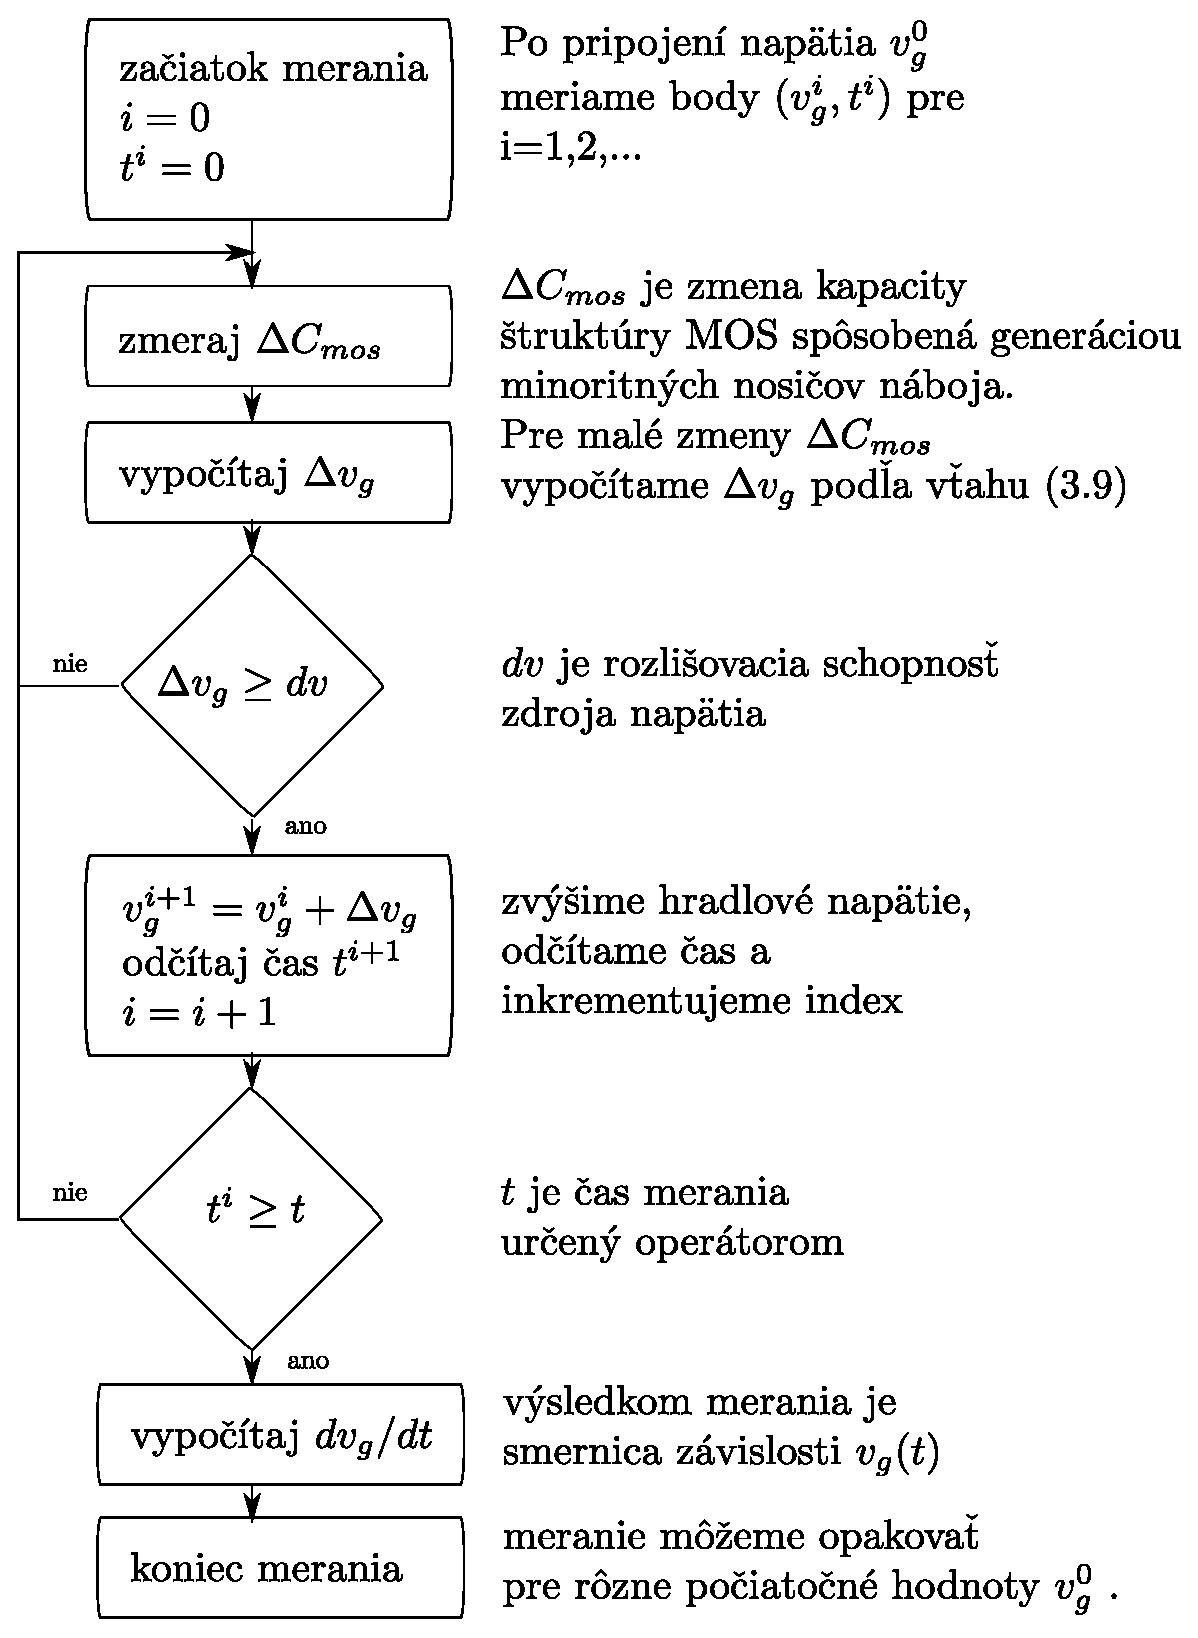
\includegraphics[scale=0.55,keepaspectratio]{Figures/diagram-2.EPS}\label{diagram:2}
\end{diagram}

Na obrázku~\ref{fig:3.5} je znázornená závislosť $\frac{dV_g}{dt}$ od
šírky OPN\@. Za predpokladu udržania konštantnej šírky OPN sa nemenia
potenciálové pomery v polovodiči a generácia minoritných nosičov je
konštantná, z čoho vyplýva linearita závislosti $V_g(t)$.  Smernice
$\frac{dV_g}{dt}$ potom možno určiť lineárnou regresiou nameraných
závislostí $V_g(t)$. Nie je ťažké si predstaviť, že
vzťahy~\ref{eq:3.6} až~\ref{eq:3.8} predstavujú diskretizáciu
spojitého priebehu $\tau_g(x)$. Ak namerané hodnoty
$\frac{dV_g}{dt}=f(x)$ aproximujeme spojitou funkciou, môžeme vyjadriť
hĺbkový profil $\tau_g(x)$ vzťahom

\begin{equation}\label{eq:3.10}
  \tau_g(x) = \frac{qn_i}{2C_{ox}} {\Bigg[\frac{d\big[\frac{dV_g}{dt}\big]}{dx}\Bigg]}^{-1}
\end{equation}

Na obrázku~\ref{fig:3.6} je znázornený priebeh $\tau_g(x)$, vypočítaný
z nameraných dát zobrazených na obrázku~\ref{fig:3.5}.

\begin{figure}[h!]\centering
  % GNUPLOT: LaTeX picture with Postscript
\begingroup
  \makeatletter
  \providecommand\color[2][]{%
    \GenericError{(gnuplot) \space\space\space\@spaces}{%
      Package color not loaded in conjunction with
      terminal option `colourtext'%
    }{See the gnuplot documentation for explanation.%
    }{Either use 'blacktext' in gnuplot or load the package
      color.sty in LaTeX.}%
    \renewcommand\color[2][]{}%
  }%
  \providecommand\includegraphics[2][]{%
    \GenericError{(gnuplot) \space\space\space\@spaces}{%
      Package graphicx or graphics not loaded%
    }{See the gnuplot documentation for explanation.%
    }{The gnuplot epslatex terminal needs graphicx.sty or graphics.sty.}%
    \renewcommand\includegraphics[2][]{}%
  }%
  \providecommand\rotatebox[2]{#2}%
  \@ifundefined{ifGPcolor}{%
    \newif\ifGPcolor
    \GPcolortrue
  }{}%
  \@ifundefined{ifGPblacktext}{%
    \newif\ifGPblacktext
    \GPblacktexttrue
  }{}%
  % define a \g@addto@macro without @ in the name:
  \let\gplgaddtomacro\g@addto@macro
  % define empty templates for all commands taking text:
  \gdef\gplbacktext{}%
  \gdef\gplfronttext{}%
  \makeatother
  \ifGPblacktext
    % no textcolor at all
    \def\colorrgb#1{}%
    \def\colorgray#1{}%
  \else
    % gray or color?
    \ifGPcolor
      \def\colorrgb#1{\color[rgb]{#1}}%
      \def\colorgray#1{\color[gray]{#1}}%
      \expandafter\def\csname LTw\endcsname{\color{white}}%
      \expandafter\def\csname LTb\endcsname{\color{black}}%
      \expandafter\def\csname LTa\endcsname{\color{black}}%
      \expandafter\def\csname LT0\endcsname{\color[rgb]{1,0,0}}%
      \expandafter\def\csname LT1\endcsname{\color[rgb]{0,1,0}}%
      \expandafter\def\csname LT2\endcsname{\color[rgb]{0,0,1}}%
      \expandafter\def\csname LT3\endcsname{\color[rgb]{1,0,1}}%
      \expandafter\def\csname LT4\endcsname{\color[rgb]{0,1,1}}%
      \expandafter\def\csname LT5\endcsname{\color[rgb]{1,1,0}}%
      \expandafter\def\csname LT6\endcsname{\color[rgb]{0,0,0}}%
      \expandafter\def\csname LT7\endcsname{\color[rgb]{1,0.3,0}}%
      \expandafter\def\csname LT8\endcsname{\color[rgb]{0.5,0.5,0.5}}%
    \else
      % gray
      \def\colorrgb#1{\color{black}}%
      \def\colorgray#1{\color[gray]{#1}}%
      \expandafter\def\csname LTw\endcsname{\color{white}}%
      \expandafter\def\csname LTb\endcsname{\color{black}}%
      \expandafter\def\csname LTa\endcsname{\color{black}}%
      \expandafter\def\csname LT0\endcsname{\color{black}}%
      \expandafter\def\csname LT1\endcsname{\color{black}}%
      \expandafter\def\csname LT2\endcsname{\color{black}}%
      \expandafter\def\csname LT3\endcsname{\color{black}}%
      \expandafter\def\csname LT4\endcsname{\color{black}}%
      \expandafter\def\csname LT5\endcsname{\color{black}}%
      \expandafter\def\csname LT6\endcsname{\color{black}}%
      \expandafter\def\csname LT7\endcsname{\color{black}}%
      \expandafter\def\csname LT8\endcsname{\color{black}}%
    \fi
  \fi
    \setlength{\unitlength}{0.0500bp}%
    \ifx\gptboxheight\undefined%
      \newlength{\gptboxheight}%
      \newlength{\gptboxwidth}%
      \newsavebox{\gptboxtext}%
    \fi%
    \setlength{\fboxrule}{0.5pt}%
    \setlength{\fboxsep}{1pt}%
\begin{picture}(7920.00,5616.00)%
    \gplgaddtomacro\gplbacktext{%
      \csname LTb\endcsname%%
      \put(980,640){\makebox(0,0)[r]{\strut{}$0.01$}}%
      \put(980,1265){\makebox(0,0)[r]{\strut{}$0.012$}}%
      \put(980,1890){\makebox(0,0)[r]{\strut{}$0.014$}}%
      \put(980,2515){\makebox(0,0)[r]{\strut{}$0.016$}}%
      \put(980,3140){\makebox(0,0)[r]{\strut{}$0.018$}}%
      \put(980,3765){\makebox(0,0)[r]{\strut{}$0.02$}}%
      \put(980,4390){\makebox(0,0)[r]{\strut{}$0.022$}}%
      \put(980,5015){\makebox(0,0)[r]{\strut{}$0.024$}}%
      \put(1100,440){\makebox(0,0){\strut{}$0$}}%
      \put(2274,440){\makebox(0,0){\strut{}$0.2$}}%
      \put(3449,440){\makebox(0,0){\strut{}$0.4$}}%
      \put(4623,440){\makebox(0,0){\strut{}$0.6$}}%
      \put(5797,440){\makebox(0,0){\strut{}$0.8$}}%
      \put(6972,440){\makebox(0,0){\strut{}$1$}}%
    }%
    \gplgaddtomacro\gplfronttext{%
      \csname LTb\endcsname%%
      \put(190,2827){\rotatebox{-270}{\makebox(0,0){\strut{}${dV_g}/{dt} \quad  [{Vs}^{-1}]$}}}%
      \put(4329,140){\makebox(0,0){\strut{}Hĺbka $[\mu{m}]$}}%
      \put(4329,5315){\makebox(0,0){\strut{}Metóda konštantnej šírky OPN.}}%
    }%
    \gplbacktext
    \put(0,0){\includegraphics{/export/scratch/vbotka-thesis/Plot/Figures/fig-3-5-sk}}%
    \gplfronttext
  \end{picture}%
\endgroup

  \caption[Závislosť $\frac{dV_g}{dt}$ od šírky OPN získaná pomocou
    metódy konštantnej šírky OPN]{Závislosť $\frac{dV_g}{dt}$ od šírky
    OPN získaná pomocou metódy konštantnej šírky OPN.}\label{fig:3.5}
\end{figure}
%OBR19.BIT

\begin{figure}[h!]\centering
  % GNUPLOT: LaTeX picture with Postscript
\begingroup
  \makeatletter
  \providecommand\color[2][]{%
    \GenericError{(gnuplot) \space\space\space\@spaces}{%
      Package color not loaded in conjunction with
      terminal option `colourtext'%
    }{See the gnuplot documentation for explanation.%
    }{Either use 'blacktext' in gnuplot or load the package
      color.sty in LaTeX.}%
    \renewcommand\color[2][]{}%
  }%
  \providecommand\includegraphics[2][]{%
    \GenericError{(gnuplot) \space\space\space\@spaces}{%
      Package graphicx or graphics not loaded%
    }{See the gnuplot documentation for explanation.%
    }{The gnuplot epslatex terminal needs graphicx.sty or graphics.sty.}%
    \renewcommand\includegraphics[2][]{}%
  }%
  \providecommand\rotatebox[2]{#2}%
  \@ifundefined{ifGPcolor}{%
    \newif\ifGPcolor
    \GPcolortrue
  }{}%
  \@ifundefined{ifGPblacktext}{%
    \newif\ifGPblacktext
    \GPblacktexttrue
  }{}%
  % define a \g@addto@macro without @ in the name:
  \let\gplgaddtomacro\g@addto@macro
  % define empty templates for all commands taking text:
  \gdef\gplbacktext{}%
  \gdef\gplfronttext{}%
  \makeatother
  \ifGPblacktext
    % no textcolor at all
    \def\colorrgb#1{}%
    \def\colorgray#1{}%
  \else
    % gray or color?
    \ifGPcolor
      \def\colorrgb#1{\color[rgb]{#1}}%
      \def\colorgray#1{\color[gray]{#1}}%
      \expandafter\def\csname LTw\endcsname{\color{white}}%
      \expandafter\def\csname LTb\endcsname{\color{black}}%
      \expandafter\def\csname LTa\endcsname{\color{black}}%
      \expandafter\def\csname LT0\endcsname{\color[rgb]{1,0,0}}%
      \expandafter\def\csname LT1\endcsname{\color[rgb]{0,1,0}}%
      \expandafter\def\csname LT2\endcsname{\color[rgb]{0,0,1}}%
      \expandafter\def\csname LT3\endcsname{\color[rgb]{1,0,1}}%
      \expandafter\def\csname LT4\endcsname{\color[rgb]{0,1,1}}%
      \expandafter\def\csname LT5\endcsname{\color[rgb]{1,1,0}}%
      \expandafter\def\csname LT6\endcsname{\color[rgb]{0,0,0}}%
      \expandafter\def\csname LT7\endcsname{\color[rgb]{1,0.3,0}}%
      \expandafter\def\csname LT8\endcsname{\color[rgb]{0.5,0.5,0.5}}%
    \else
      % gray
      \def\colorrgb#1{\color{black}}%
      \def\colorgray#1{\color[gray]{#1}}%
      \expandafter\def\csname LTw\endcsname{\color{white}}%
      \expandafter\def\csname LTb\endcsname{\color{black}}%
      \expandafter\def\csname LTa\endcsname{\color{black}}%
      \expandafter\def\csname LT0\endcsname{\color{black}}%
      \expandafter\def\csname LT1\endcsname{\color{black}}%
      \expandafter\def\csname LT2\endcsname{\color{black}}%
      \expandafter\def\csname LT3\endcsname{\color{black}}%
      \expandafter\def\csname LT4\endcsname{\color{black}}%
      \expandafter\def\csname LT5\endcsname{\color{black}}%
      \expandafter\def\csname LT6\endcsname{\color{black}}%
      \expandafter\def\csname LT7\endcsname{\color{black}}%
      \expandafter\def\csname LT8\endcsname{\color{black}}%
    \fi
  \fi
    \setlength{\unitlength}{0.0500bp}%
    \ifx\gptboxheight\undefined%
      \newlength{\gptboxheight}%
      \newlength{\gptboxwidth}%
      \newsavebox{\gptboxtext}%
    \fi%
    \setlength{\fboxrule}{0.5pt}%
    \setlength{\fboxsep}{1pt}%
\begin{picture}(7920.00,5616.00)%
    \gplgaddtomacro\gplbacktext{%
      \csname LTb\endcsname%%
      \put(740,640){\makebox(0,0)[r]{\strut{}$0.2$}}%
      \put(740,1369){\makebox(0,0)[r]{\strut{}$0.4$}}%
      \put(740,2098){\makebox(0,0)[r]{\strut{}$0.6$}}%
      \put(740,2828){\makebox(0,0)[r]{\strut{}$0.8$}}%
      \put(740,3557){\makebox(0,0)[r]{\strut{}$1$}}%
      \put(740,4286){\makebox(0,0)[r]{\strut{}$1.2$}}%
      \put(740,5015){\makebox(0,0)[r]{\strut{}$1.4$}}%
      \put(860,440){\makebox(0,0){\strut{}$0$}}%
      \put(2078,440){\makebox(0,0){\strut{}$0.2$}}%
      \put(3296,440){\makebox(0,0){\strut{}$0.4$}}%
      \put(4514,440){\makebox(0,0){\strut{}$0.6$}}%
      \put(5732,440){\makebox(0,0){\strut{}$0.8$}}%
      \put(6950,440){\makebox(0,0){\strut{}$1$}}%
    }%
    \gplgaddtomacro\gplfronttext{%
      \csname LTb\endcsname%%
      \put(190,2827){\rotatebox{-270}{\makebox(0,0){\strut{}${\tau}_{g}$ $[ms]$}}}%
      \put(4209,140){\makebox(0,0){\strut{}Hĺbka $[\mu{m}]$}}%
      \put(4209,5315){\makebox(0,0){\strut{}Generačný čas života minoritných nosičov náboja}}%
    }%
    \gplbacktext
    \put(0,0){\includegraphics{/export/scratch/vbotka-thesis/Plot/Figures/fig-3-6-sk}}%
    \gplfronttext
  \end{picture}%
\endgroup

  \caption[Hĺbkový profil generačného času života minoritných nosičov
  náboja]{Hĺbkový profil generačného času života minoritných nosičov
  náboja.}\label{fig:3.6}
\end{figure}
%OBR20.BIT

Na obrázku~\ref{fig:3.7} je nameraný hĺbkový koncentračný profil
$N(x)$ skúmanej štruktúry.

\begin{figure}[h!]\centering
  % GNUPLOT: LaTeX picture with Postscript
\begingroup
  \makeatletter
  \providecommand\color[2][]{%
    \GenericError{(gnuplot) \space\space\space\@spaces}{%
      Package color not loaded in conjunction with
      terminal option `colourtext'%
    }{See the gnuplot documentation for explanation.%
    }{Either use 'blacktext' in gnuplot or load the package
      color.sty in LaTeX.}%
    \renewcommand\color[2][]{}%
  }%
  \providecommand\includegraphics[2][]{%
    \GenericError{(gnuplot) \space\space\space\@spaces}{%
      Package graphicx or graphics not loaded%
    }{See the gnuplot documentation for explanation.%
    }{The gnuplot epslatex terminal needs graphicx.sty or graphics.sty.}%
    \renewcommand\includegraphics[2][]{}%
  }%
  \providecommand\rotatebox[2]{#2}%
  \@ifundefined{ifGPcolor}{%
    \newif\ifGPcolor
    \GPcolortrue
  }{}%
  \@ifundefined{ifGPblacktext}{%
    \newif\ifGPblacktext
    \GPblacktexttrue
  }{}%
  % define a \g@addto@macro without @ in the name:
  \let\gplgaddtomacro\g@addto@macro
  % define empty templates for all commands taking text:
  \gdef\gplbacktext{}%
  \gdef\gplfronttext{}%
  \makeatother
  \ifGPblacktext
    % no textcolor at all
    \def\colorrgb#1{}%
    \def\colorgray#1{}%
  \else
    % gray or color?
    \ifGPcolor
      \def\colorrgb#1{\color[rgb]{#1}}%
      \def\colorgray#1{\color[gray]{#1}}%
      \expandafter\def\csname LTw\endcsname{\color{white}}%
      \expandafter\def\csname LTb\endcsname{\color{black}}%
      \expandafter\def\csname LTa\endcsname{\color{black}}%
      \expandafter\def\csname LT0\endcsname{\color[rgb]{1,0,0}}%
      \expandafter\def\csname LT1\endcsname{\color[rgb]{0,1,0}}%
      \expandafter\def\csname LT2\endcsname{\color[rgb]{0,0,1}}%
      \expandafter\def\csname LT3\endcsname{\color[rgb]{1,0,1}}%
      \expandafter\def\csname LT4\endcsname{\color[rgb]{0,1,1}}%
      \expandafter\def\csname LT5\endcsname{\color[rgb]{1,1,0}}%
      \expandafter\def\csname LT6\endcsname{\color[rgb]{0,0,0}}%
      \expandafter\def\csname LT7\endcsname{\color[rgb]{1,0.3,0}}%
      \expandafter\def\csname LT8\endcsname{\color[rgb]{0.5,0.5,0.5}}%
    \else
      % gray
      \def\colorrgb#1{\color{black}}%
      \def\colorgray#1{\color[gray]{#1}}%
      \expandafter\def\csname LTw\endcsname{\color{white}}%
      \expandafter\def\csname LTb\endcsname{\color{black}}%
      \expandafter\def\csname LTa\endcsname{\color{black}}%
      \expandafter\def\csname LT0\endcsname{\color{black}}%
      \expandafter\def\csname LT1\endcsname{\color{black}}%
      \expandafter\def\csname LT2\endcsname{\color{black}}%
      \expandafter\def\csname LT3\endcsname{\color{black}}%
      \expandafter\def\csname LT4\endcsname{\color{black}}%
      \expandafter\def\csname LT5\endcsname{\color{black}}%
      \expandafter\def\csname LT6\endcsname{\color{black}}%
      \expandafter\def\csname LT7\endcsname{\color{black}}%
      \expandafter\def\csname LT8\endcsname{\color{black}}%
    \fi
  \fi
    \setlength{\unitlength}{0.0500bp}%
    \ifx\gptboxheight\undefined%
      \newlength{\gptboxheight}%
      \newlength{\gptboxwidth}%
      \newsavebox{\gptboxtext}%
    \fi%
    \setlength{\fboxrule}{0.5pt}%
    \setlength{\fboxsep}{1pt}%
\begin{picture}(7920.00,5616.00)%
    \gplgaddtomacro\gplbacktext{%
      \csname LTb\endcsname%%
      \put(1100,1299){\makebox(0,0)[r]{\strut{}$1\times10^{21}$}}%
      \put(1100,3486){\makebox(0,0)[r]{\strut{}$1\times10^{22}$}}%
      \put(1220,440){\makebox(0,0){\strut{}$0$}}%
      \put(2373,440){\makebox(0,0){\strut{}$0.2$}}%
      \put(3525,440){\makebox(0,0){\strut{}$0.4$}}%
      \put(4678,440){\makebox(0,0){\strut{}$0.6$}}%
      \put(5830,440){\makebox(0,0){\strut{}$0.8$}}%
      \put(6983,440){\makebox(0,0){\strut{}$1$}}%
    }%
    \gplgaddtomacro\gplfronttext{%
      \csname LTb\endcsname%%
      \put(190,2827){\rotatebox{-270}{\makebox(0,0){\strut{}Koncentrácia $[{m}^{-3}]$}}}%
      \put(4389,140){\makebox(0,0){\strut{}Hĺbka $[\mu{m}]$}}%
      \put(4389,5315){\makebox(0,0){\strut{}Kocentrácia dopantov}}%
    }%
    \gplbacktext
    \put(0,0){\includegraphics{/export/scratch/vbotka-thesis/Plot/Figures/fig-3-7-sk}}%
    \gplfronttext
  \end{picture}%
\endgroup

  \caption[Hĺbkový profil koncentrácie dotujúcich prímesí
  $N(x)$]{Hĺbkový profil koncentrácie dotujúcich prímesí
  $N(x)$. Koncentračný profil prímesí bol vytvorený implantáciou
  $P^{31}$ s dávkou $8.0$ $10^{15}m^{-2}$ pri energii $120 keV$.
  Aktivácia prebiehala počas 40 minút pri teplote $1050 \degree C$ v
  atmosfére $N_2$.}\label{fig:3.7}
\end{figure}
%OBR21.BIT


\begin{thebibliography}{}

\bibitem[3.1]{3.1}
Pierret R.F., Small D.W.: IEEE Trans.\ on elektron.dev. 22 (1975) s.1052.

\bibitem[3.2]{3.2}
Zerbst M.: Z. Angew. Phys. 22 (1966), s.30.

\bibitem[3.3]{3.3}
Eades W.D., Shott J.D., Swanson R.M.: IEEE Trans.\ on elektron.\ dev. 30 (1983) s.1274.

\bibitem[3.4]{3.4}
Nicollian E.H., Brews J.R.: Solid St.\ Electron.  27 (1984) s.953.

\bibitem[3.5]{3.5}
Ziegler K., Klausmann E.: Appl. Phys. Lett. 26 (1975) s.400.

\bibitem[3.6]{3.6}
Boulin D.M., Brews J.R., Nicollian E.H.: Solid St.\ Electron. 27  (1984) s.977.

\bibitem[3.7]{3.7}
Brews J.R., Nicollian E.H.: Solid  St.\ Electron. 27 (1984) s.963.

\bibitem[3.8]{3.8}
Botka V.,Csabay O., Jamrich M.: 5.celoštátna konferencia Mikroelektronika 1989, Dom techniky ČSVTS Bratislava, 1989 s.59.

\bibitem[3.9]{3.9}
Jamrich M.: Q-C metóda pre skúmanie štruktúr MIS\@. Diplomová práca, Katedra mikroelektroniky, EF SVŠT, Bratislava 1988.

\bibitem[3.10]{3.10}
Beyer A., Markgraf W.: Wiss. Z. d. Techn. Hochsch. Karl-Marx-Stadt 28 (1986) s.479.

\bibitem[3.11]{3.11}
Lal, Vasi: Solid St.\ Electron. 30 (1987) s.801.

\bibitem[3.12]{3.12}
Hof, Morthers, Roenker: Solid St.\ Electron. 31 (1988) s.937.

\bibitem[3.13]{3.13}
Pilka K.: Nerovnovážna kapacitná metóda s konštantnou šírkou OPN, Katedra mikroelektroniky, EF SVŠT, Bratislava 1989.

\end{thebibliography}

% Chapter 4

\chapter{Metódy určenia ďalších parametrov štruktúry MOS.}\label{Chapter4}
\lhead{Chapter 4. \emph{Metódy určenia ďalších parametrov štruktúry MOS}}
%- - - - - - - - - - - - - - - - - - - - - - - - - - - - - - - - - - - - -

V kapitole~\ref{Chapter3} sme popísali C-V metódy, ktoré budeme
používať na určovanie parametrov štruktúr MOS\@. Predovšetkým sa
budeme zaoberať určením koncentračného profilu dotujúcich prímesí v
podpovrchovej oblasti polovodiča, pretože niektoré metódy určovania
ďalších parametrov štruktúry MOS vychádzajú z predpokladu, že priebeh
koncentrácie je známy. Pri určovaní priebehov koncentračných profilov,
ktoré nie su homogénne, sa používajú modely, ktorých presnosť
aproximácie daného fyzikálneho javu závisí od gradientu koncentrácie
prímesí~\cite{4.1, 4.2, 4.3, 4.4}. Aby sme overili presnosť použitých
aproximácií, vykonali sme porovnanie koncentračných profilov:

\begin{itemize}
\item použitého pri výpočte teoretickej C-V závislosti a
\item získaného z tejto teoretickej C-V závislosti~\cite{4.5}.
\end{itemize}

Výsledky sú uvedené v časti~\ref{sec:4.1.4}.

\par Ďalším parametrom, ktorý budeme určovať, je hustota pascí
rozhrania $Si-SiO_{2}$. Tu prichádzajú do úvahy dva
postupy. Porovnanie vysokofrekvenčnej a nízkofrekvenčnej C-V
závislosti, alebo porovnanie experimentálnej a teoretickej C-V
závislosti. Ich aplikácia je popísana v časti~\ref{sec:4.2}.

\par Určenie generačného času života minoritných nosičov náboja, ktoré
súvisí s metódou konštantnej šírky OPN, bolo popísané v
časti~\ref{sec:3.4}.

\section[Určenie koncentračného profilu prímesí]{Určenie koncentračného profilu prímesí v podpovrchovej oblasti polovodiča.}\label{sec:4.1}

Problematika merania koncentračných profilov bola na našom oddelení
spracovaná v práci~\cite{4.6}. Tu sa budeme zaoberať len niektorými
aspektmi tejto problematiky, ktoré súvisia s určením nehomogénneho
koncentračného profilu prímesí v polovodiči.

\par Samostatné okruhy problémov pri určovaní koncentračného profilu
prímesí, ktorý označíme $N(x)$, tvoria:

\begin{itemize}
\item korekcia vypočítanej koncentrácie v oblasti od povrchu
  polovodiča do hĺbky $2L_{DE}$~\cite{4.7, 4.8}
\item určenie hĺbky vypočítanej koncentrácie, opierajúca sa o modely
  určenia šírky OPN~\cite{4.9, 4.10, 4.11}
\item korekcia vplyvu pascí rozhrania $Si-SiO_2$~\cite{4.12}
\item rozdiel medzi koncentráciou dotujúcich prímesí $N(x)$ a
  koncentráciou majoritných nosičov náboja $n(x)$.
\end{itemize}

Postupne sa budeme zaoberať uvedenými okruhmi problémov.

\subsection[Korekcia koncentrácie dotujúcich prímesí]{Korekcia koncentrácie dotujúcich prímesí pri povrchu polovodiča.}\label{sec:4.1.1}

Známy vzťah pre výpočet $N(x)$~\cite{I.2}

\begin{equation}\label{eq:4.1}
  N(x) = {\frac{2}{q\epsilon}} {\Bigg[\frac{dC_{sc}^{-2}}{d\varphi_{s}}\Bigg]}^{-1}
\end{equation}

bol odvodený z riešenia Poissonovej rovnice s použitím aproximácie
hlbokého ochudobnenia. Táto aproximácia neplatí pre šírku OPN menšiu
ako $2L_{DE}$.  Aby sme dosiahli správne výsledky aj v tejto oblasti,
musíme $N(x)$ vypočítané podľa~\ref{eq:4.1} korigovať postupom
odvodeným v~\cite{4.7, 4.8}. Z práce~\cite{4.7} je zrejmý aj
fyzikálny význam tejto korekcie, ktorá je funkciou povrchového
potenciálu

\begin{equation}\label{eq:4.2}
  {N(x)}_{korigovane} = N(x)f(\varphi_{s})
\end{equation}

, kde

\begin{equation}\label{eq:4.3}
  f(\varphi_{s}) = {\frac{1}{1-e^{-\beta\varphi_{s}}}} - {\frac{2e^{-\beta\varphi_{s}}\big[e^{-\beta\varphi_{s}}+\beta\varphi_{s} - 1\big]}{\big[1 - e^{-\beta\varphi_{s}}\big]}} \qquad,kde\quad \beta=\frac{q}{kT}
\end{equation}

Povrchový potenciál, použitý vo vzťahu~\ref{eq:4.3} možno určiť
podla~\cite{4.7} numerickým riešením rovnice

\begin{equation}\label{eq:4.4}
  \frac{C_{sc}^{2}}{\varphi_{s}}\frac{C_{sc}^{-2}}{d\varphi_{s}}=\frac{1-e^{-\beta\varphi_{s}}}{e^{-\beta\varphi_{s}}+\beta\varphi_{s}-1}-\frac{2e^{-\beta\varphi_{s}}} {1-e^{-\beta\varphi_{s}}}
\end{equation}

Tu treba poznamenať, že vzťah~\ref{eq:4.4} bol odvodený pomocou vzťahu
pre kapacitu OPN $C_{sc}$, ktorý predpokladá homogénnu koncentráciu
prímesí. Pretože experimentálne zistená diferenciálna kapacita
$C_{sc}$ závisí od zmeny náboja na hranici OPN (čo využíva
vzťah~\ref{eq:4.1}), bude povrchový potenciál získaný zo
vzťahu~\ref{eq:4.4} predstavovať potenciál, ktorý by bol na povrchu
polovodiča, ak by koncentrácia $N(x)$ v celej oblasti OPN bola
konštantná a zároveň rovná koncentrácii na hranici OPN (ktorú určujeme
podľa~\ref{eq:4.1}). Z uvedeného vyplýva, že pre nehomogénne dotované
substráty pomocou vzťahu~\ref{eq:4.4} nemožno získať skutočný priebeh
$\varphi_{s}(V_{g})$, napriek tomu, že korekcia~\ref{eq:4.2} dáva
dobré výsledky aj v tomto prípade.

\subsection[Určenie hĺbky koncentračného profilu.]{Určenie hĺbky koncentračného profilu.}\label{sec:4.1.2}

Po určení koncentrácie podľa vzťahu~\ref{eq:4.2} treba zároveň určiť
polohu vypočítanej koncentrácie. Bežne používaný vzťah vychádzajúci z
modelu doskového kondenzátora (čo predstavuje aproximáciu hlbokého
ochudobnenia)

\begin{equation}\label{eq:4.5}
  w(C_{sc})=\frac{\epsilon}{C_{sc}}
\end{equation}

neplatí pre hĺbky menšie ako $2L_{DE}$. V tejto oblasti možno použiť
vzťah odvodený pomocou aproximácie priebehu potenciálu v polovodiči
$\varphi(x)$. Uvedená problematika bola na našom oddelení podrobne
spracovaná v~\cite{4.13, 4.14}, keď boli použité výsledky
prác~\cite{4.9, 4.10, 4.11}. Pre výpočet hĺbky v tejto oblasti môžeme
použiť vzťah, ktorý predstavuje aproximáciu priebehu potenciálu v
polovodiči $\varphi(x)$~\cite{I.1}

\begin{equation}\label{eq:4.6}
  w(\varphi_{s})=\sqrt{2}L_{DE}{\big[e^{-\beta\varphi_{s}}+\beta\varphi_{s}-1\big]}^{\frac{1}{2}}
\end{equation}

, kde 

\begin{equation}\label{eq:4.7}
  L_{DE} = {\Big[\frac{\epsilon}{\beta qN}\Big]}^{\frac{1}{2}}
\end{equation}

je extrinzická Debayova dĺžka, pri výpočte ktorej sme použili
koncentráciu získanú zo vzťahu~\ref{eq:4.2}.  Vo vzťahu~\ref{eq:4.6}
použijeme hodnotu $\varphi_{s}$ získanú z riešenia
vzťahu~\ref{eq:4.4}.  Napriek tomu, že aj vzťah~\ref{eq:4.6} bol
odvodený za predpokladu homogénneho rozloženia prímesí v polovodiči,
jeho použitie v spojení s riešení rovnice~\ref{eq:4.4} dáva uspokojivé
výsledky, ako ukážeme neskôr.

\begin{figure}[h!]\centering
  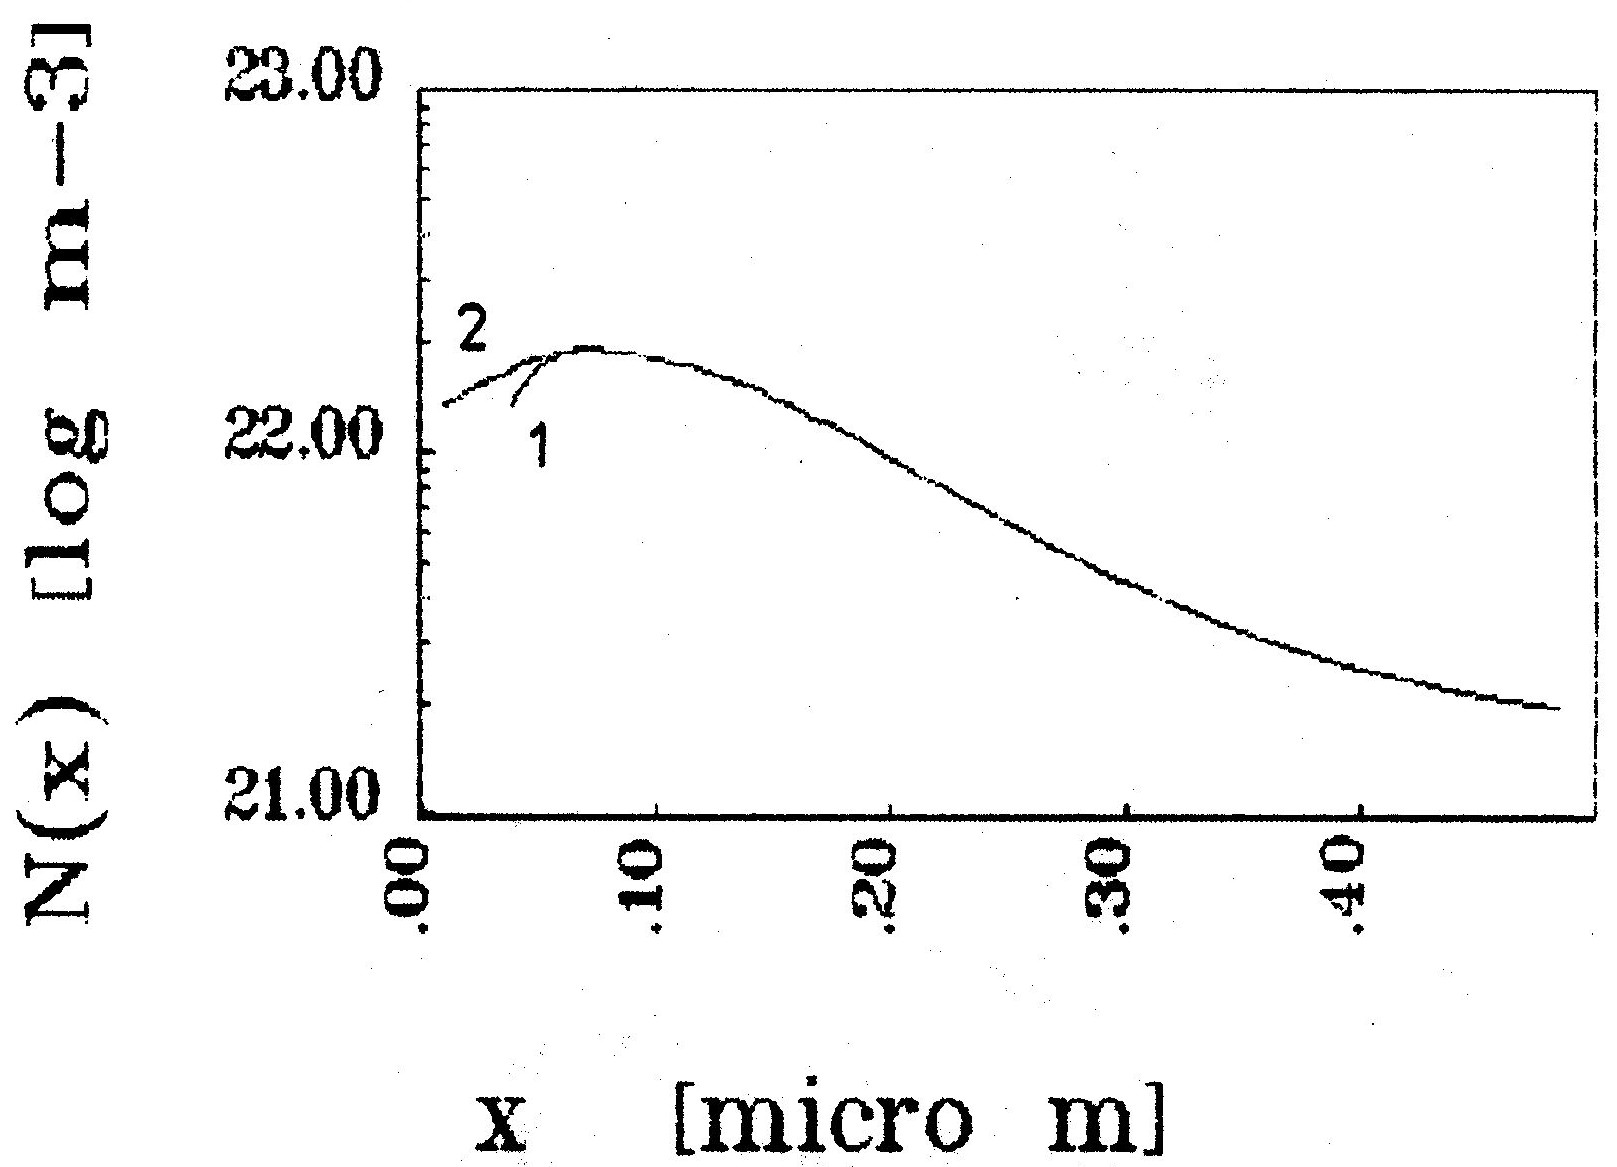
\includegraphics{Figures/fig-4-1.eps}% chktex-file 8
  \caption[Priebeh koncentrácie dotujúcich prímesí v polovodiči
    vypočítaný zo vzťahu~\ref{eq:4.2}]{Priebeh koncentrácie dotujúcich
    prímesí v polovodiči vypočítaný zo
    vzťahu~\ref{eq:4.2}. Vzdialenosť od povrchu bola určená zo
    vzťahov~\ref{eq:4.5} (krivka 1) a~\ref{eq:4.6} (krivka
    2).}\label{fig:4.1}
\end{figure}
% OBR26.BIT

Na obrázku~\ref{fig:4.1} sú znázornené priebehy $N(x)$ s použitím
korekcie~\ref{eq:4.2}, prezentujúce rozdiel v použití
vzťahov~\ref{eq:4.5} a~\ref{eq:4.6}. Tu je zrejmé, že použitím
vzťahu~\ref{eq:4.6} možno vypočítať priebeh koncentrácie dotujúcich
prímesí bližšie k povrchu polovodiča, čo má význam pre ďalšie výpočty,
ktoré predpokladajú znalosť priebehu $N(x)$.

Prvý stĺpec tabulky~\ref{tab:4.1} obsahuje hodnoty $\varphi_{s}$
určené riešením rovnice~\ref{eq:4.4} a v druhom stĺpci sa nachádzajú
hodnoty korekčného faktora~\ref{eq:4.3}. Ďalšie dva stĺpce umožňujú
porovnanie nekorigovanej a korigovanej hodnoty $N(x)$ a v posledných
dvoch stĺpcoch sú uvedené hodnoty $w(\varphi_{s})$ a $w(C_{sc})$
získané zo vzťahov~\ref{eq:4.5} a~\ref{eq:4.6}.

\begin{table}[h!]\centering
  \begin{tabular}{c c c c c c}
  $\varphi_{s}[V]$ & $f(\varphi_{s})$ & $N[m^{-3}]$ & $N_{kor.}[m^{-3}]$ & $w(\varphi_{s})[\mu m]$ & $w(C_{SC})[\mu m]$ \\
  \hline% chktex-file 44
  0.007 & 0.39 & $0.35\times10^{23}$ & $0.14\times10^{23}$ & 0.0102 & 0.0389 \\
  0.016 & 0.44 & $0.33\times10^{23}$ & $0.15\times10^{23}$ & 0.0190 & 0.0413 \\
  0.024 & 0.50 & $0.31\times10^{23}$ & $0.15\times10^{23}$ & 0.0265 & 0.0438 \\
  0.032 & 0.56 & $0.29\times10^{23}$ & $0.16\times10^{23}$ & 0.0333 & 0.0466 \\
  0.041 & 0.61 & $0.28\times10^{23}$ & $0.17\times10^{23}$ & 0.0391 & 0.0494 \\
  0.049 & 0.66 & $0.27\times10^{23}$ & $0.18\times10^{23}$ & 0.0444 & 0.0523 \\
  0.057 & 0.71 & $0.26\times10^{23}$ & $0.18\times10^{23}$ & 0.0493 & 0.0553 \\
  0.065 & 0.76 & $0.25\times10^{23}$ & $0.19\times10^{23}$ & 0.0538 & 0.0585 \\
  0.073 & 0.80 & $0.24\times10^{23}$ & $0.19\times10^{23}$ & 0.0581 & 0.0617 \\
  0.081 & 0.83 & $0.23\times10^{23}$ & $0.19\times10^{23}$ & 0.0623 & 0.0650 \\
  0.090 & 0.86 & $0.22\times10^{23}$ & $0.19\times10^{23}$ & 0.0664 & 0.0684 \\
  0.098 & 0.89 & $0.22\times10^{23}$ & $0.19\times10^{23}$ & 0.0704 & 0.0719 \\
  0.106 & 0.91 & $0.21\times10^{23}$ & $0.19\times10^{23}$ & 0.0743 & 0.0755 \\
  0.115 & 0.93 & $0.21\times10^{23}$ & $0.19\times10^{23}$ & 0.0783 & 0.0791 \\
  0.124 & 0.94 & $0.20\times10^{23}$ & $0.19\times10^{23}$ & 0.0822 & 0.0828 \\
  0.133 & 0.96 & $0.20\times10^{23}$ & $0.19\times10^{23}$ & 0.0861 & 0.0866 \\
  0.142 & 0.97 & $0.19\times10^{23}$ & $0.19\times10^{23}$ & 0.0900 & 0.0904 \\
  0.151 & 0.97 & $0.19\times10^{23}$ & $0.18\times10^{23}$ & 0.0939 & 0.0942 \\
  0.160 & 0.98 & $0.19\times10^{23}$ & $0.18\times10^{23}$ & 0.0978 & 0.0981 \\
  0.169 & 0.99 & $0.18\times10^{23}$ & $0.18\times10^{23}$ & 0.1018 & 0.1019 \\
  0.178 & 0.99 & $0.18\times10^{23}$ & $0.18\times10^{23}$ & 0.1058 & 0.1058 \\
  0.187 & 0.99 & $0.18\times10^{23}$ & $0.17\times10^{23}$ & 0.1098 & 0.1098 \\
  0.205 & 1.00 & $0.17\times10^{23}$ & $0.17\times10^{23}$ & 0.1179 & 0.1179 \\
  \end{tabular}
  \caption[Výpočet koncentračného profilu prímesí $N(x)$]{Výpočet
    koncentračného profilu prímesí $N(x)$.}\label{tab:4.1}
\end{table}

\emph{POZNÁMKA.}

Pomocou aproximácie~\ref{eq:4.6}, ktorá predstavuje šírku OPN ako
funkciu povrchového potenciaálu polovodiča (koncentrácia je
parameter), možno aproximovať priebeh $\varphi(x)$ pre danú šírku OPN
aj v prípade, že substrát polovodiča je nehomogénne dotovaný.  Vlastný
postup určenia koncentrácie dotujúcich prímesí z kapacitného merania
predstavuje diskretizáciu spojitého priebehu $N(x)$, kde jednotlivé
hodnoty $N_i$ predstavujú aproximáciu koncentrácie v oblasti hranice
OPN~\cite{4.1, 4.2, 4.3}.  Úbytok potenciálu $\Delta\varphi_i$ na
vrstve šírky $\Delta w_{i}=w_{i+1}-w_{i}$ s koncentráciou $N_i$ možno
určiť riešením vzťahu

\begin{equation}\label{eq:4.8}
  \Delta w_{i} = \sqrt{2}L_{DE_{i}}{\Big[e^{-\beta\Delta\varphi_{i}} + \beta\Delta\varphi_{i} - 1\Big]}^{\frac{1}{2}}
\end{equation}

, kde

\begin{equation}\label{eq:4.9}
  L_{DE_{i}} = {\bigg[\frac{\epsilon}{\beta qN_{i}}\bigg]}^{\frac{1}{2}}
\end{equation}

Potom priebeh $\varphi(x)$ možno získať použitím vzťahov~\ref{eq:4.8}
a~\ref{eq:4.9} ak s výpočtom začneme od hranice OPN, kde predpokladáme
potenciál rovný nule, smerom k povrchu polovodiča.


\subsection[Vplyv pascí rozhrania $Si-SiO_{2}$ a generácie minoritných nosičov náboja.]{Vplyv pascí rozhrania $Si-SiO_{2}$ a generácie minoritných nosičov náboja}\label{sec:4.1.3}

V oblasti inverzie dochádza v OPN ku generácii minoritných nosičov
náboja, ktoré vytvárajú inverznú vrstvu a ovplyvňujú veľkost kapacity
štruktúry MOS\@. Aby sme namerali C-V závislosť v oblasti hlbokého
ochudobnenia, ktorá nie je ovplyvnená minoritnými nosičmi náboja,
použijeme impulznú HF C-V metódu. Namerané hodnoty $N(x)$ získané
pomocou tejto metódy sú na obrázku~\ref{fig:4.2}.

\begin{figure}[h!]\centering
  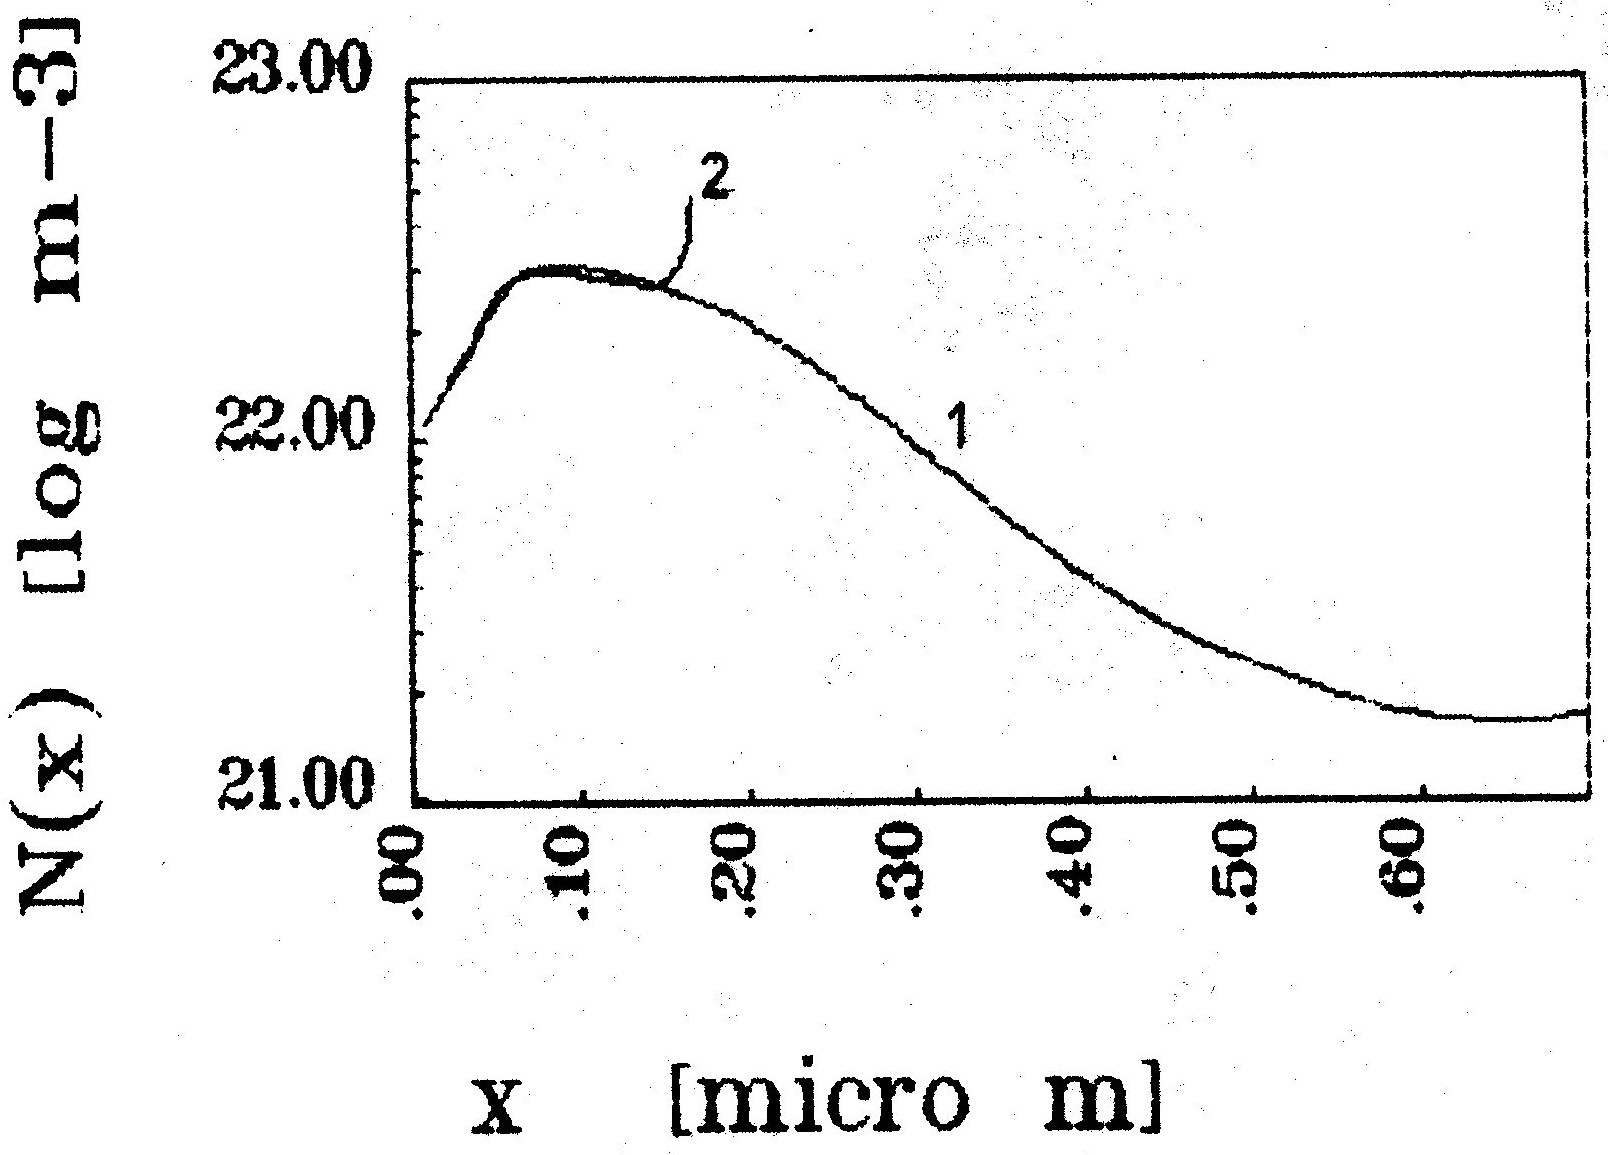
\includegraphics{Figures/fig-4-2.eps}% chktex-file 8
  \caption[Priebeh koncentračného profilu dotujúcich prímesí získaný z
    C-V závislosti v oblasti hlbokého ochudobnenia a z rovnovážnej C-V
    závislosti]{Priebeh koncentračného profilu dotujúcich prímesí
    získaný z C-V závislosti v oblasti hlbokého ochudobnenia (krivka
    1) a z rovnovážnej C-V závislosti (krivka 2). Pre výpočet
    závislosti $N(x)$ boli použité C-V závislosti zobrazené na
    obrázku~\ref{fig:3.2}}\label{fig:4.2}
\end{figure}
% OBR8.BIT

\par Pri výpočte $N(x)$ pomocou
vzťahov~\ref{eq:4.1},~\ref{eq:4.2},~\ref{eq:4.3},~\ref{eq:4.4}
a~\ref{eq:4.6} sa používa aproximácia

\begin{equation}\label{eq:4.10}
  \frac{dC_{sc}^{-2}}{d\varphi_{s}} \cong \frac{dC_{mos}^{-2}}{dV_{g}}
\end{equation}

kde rovnosť platí v prípade, že hustota pascí rozhrania $Si-SiO_{2}$
je rovná nule. Nameraná HF C-V závislosť je však vždy do určitej miery
ovplyvnená pascami rozhrania, ktoré počas merania menia svoj
stav~\cite{4.15}. Tento vplyv možno zmenšovať zvyšovaním frekvencie
meracieho signálu a rýchlejším meraním kapacity po napäťovom skoku
impulznej C-V metódy.  Problému použitia aproximácie~\ref{eq:4.10} sa
vyhneme, ak použijeme na určenie $N(x)$ dáta namerané pomocou Q-C
metódy, pri ktorej vieme určit priebeh povrchového potenciálu
$\varphi_{s}(V_{g})$.

\par Ak určujeme koncentračný profil dotujúcich prímesí z HF C-V
závislosti, môžeme vplyv pascí rozhrania $Si-SiO_{2}$ korigovať v
oblasti ochudobnenia vzťahom uvedeným v~\cite{I.1}

\begin{equation}\label{eq:4.11}
  {N(x)}_{korigovane} = {N(x)}{\frac{1-\frac{C_{mos}^{LF}}{C_{ox}}}{1-\frac{C_{mos}^{HF}}{C_{ox}}}}
\end{equation}

za predpokladu, že poznáme priebeh nízkofrekvenčnej C-V závislosti.


\subsection[Výpočet koncentračného profilu dotujúcich prímesí z priebehu majoritných nosičov náboja a overenie použitých modelov.]{Výpočet koncentračného profilu dotujúcich prímesí z priebehu majoritných nosičov náboja a overenie použitých modelov.}\label{sec:4.1.4}

Ako vidieť z obrázku~\ref{fig:1.1}, pre nehomogénny priebeh
koncentrácie dotujúcich atómov dochádza v dôsledku difúzie majoritných
nosičov náboja k rozdielu medzi uvedenými priebehmi~\cite{4.16}. Je
známe~\cite{4.17}, že pomocou vzťahu~\ref{eq:4.1} určujeme priebeh
koncentrácie majoritných nosičov náboja namiesto koncentrácie
dotujúcich prímesí. V práci~\cite{4.18} je popísaná korekcia, pomocou
ktorej možno určiť presný priebeh koncentrácie dotujúcich atómov z
nameraného priebehu $n(x)$ (ak nameraný priebeh $n(x)$ skutočne
predstavuje priebeh majoritných nosičov náboja).

\begin{figure}[h!]\centering
  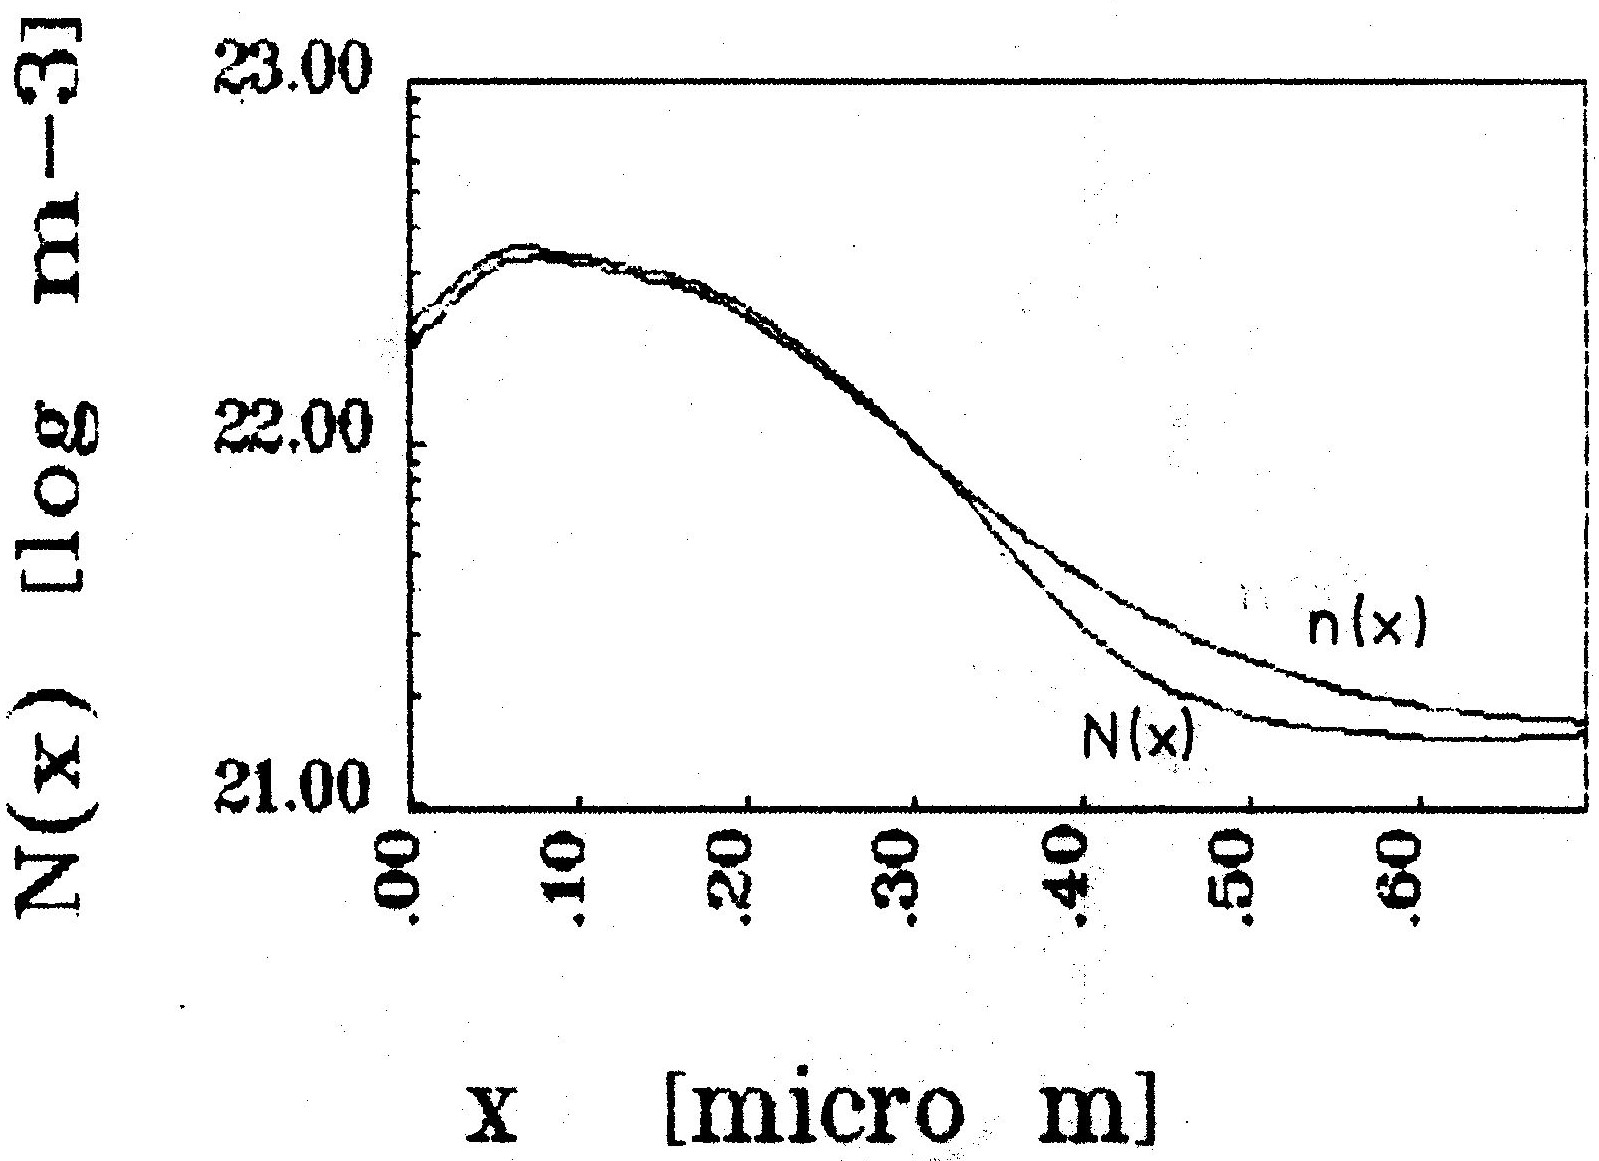
\includegraphics{Figures/fig-4-3.eps}
  \caption[Priebeh koncentrácie majoritných nosičov náboja $n(x)$
    určený z ochudobnenej HF C-V závislosti a priebeh dotujúcich
    atómov $N(x)$ určený zo vzťahu~\ref{eq:4.12}]{Priebeh koncentrácie
    majoritných nosičov náboja $n(x)$ určený z ochudobnenej HF C-V
    závislosti a priebeh dotujúcich atómov $N(x)$ určený zo
    vzťahu~\ref{eq:4.12}.}\label{fig:4.3}
\end{figure}
% OBR23.BIT

\begin{equation}\label{eq:4.12}
  N(x) = n(x) - {\frac{kT\epsilon}{q^{2}} {\frac{d}{dx}} {\Bigg[\frac{1}{n(x)}\frac{dn(x)}{dx}\Bigg]}}
\end{equation}

Na obrázku~\ref{fig:4.3} sú znázornené priebehy $n(x)$ a $N(x)$. Vo
vzťahu~\ref{eq:4.12} vystupuje druhá derivácia $n(x)$, ktorú v prípade
experimentálnych hodnôt $n(x)$ musíme určiť numericky.

\par Určovanie derivácie empiricky získanej funkčnej závislosti je
problém, s ktorým sa možno často stretnúť pri spracovaní nameraných
dát. V základných kurzoch numerickej matematiky~\cite{4.19} sa
dokazuje, že diferenciácia zosilňuje šum spracovávaných dát. Pritom
šumom tu všeobecne označujeme odchýlku spracovávaných dát od ich
skutočnej hodnoty, ktorá môže vzniknúť dôsledkom:

\begin{itemize}
\item fyzikálnych javov
\item chyby meracieho prístroja
\item zaokrúhlovania pri číslicovom spracovaní.
\end{itemize}

\par To znamená, že frekvenčné spektrum spracovávaného signálu,
získané pomocou Fourierovej transformácie, bude obsahovať zložky,
ktoré je potrebné odstránit pred (,alebo pri) výpočte derivácie. V
ďalšom budeme hovoriť o aproximácii pomocou polynómov, ktorá sa
používa najčastejšie, aj keď uvedené tvrdenia platia tiež pre iné
triedy funkcií.

\par Ak pre výpočet derivácie použijeme polynomiálne aproximácie, je
vhodné najprv funkčné hodnoty `vyhladiť'~\cite{4.20}. Pre potlačenie
šumu sú potom dôležité frekvenčné vlastnosti použitých numerických
metód, ktoré možno vyjadriť pomocou prenosovej charakteristiky. Týmto
prístupom môžeme porovnávať frekvenčné vlastnosti polynomiálnych
aproximácií a číslicových filtrov~\cite{4.21}.  Základným rozdielom
medzi výpočtom koeficientov číslicových filtrov a koeficientov
polynomiálnych aproximácií je, že v prvom prípade vychádzame z
požadovanej prenosovej charakteristiky a v druhom prípade sú
koeficienty počítané z podmienky najmenších štvorcov vzdialenosti
spracovávaných dát a polynómu daného stupňa. Z uvedeného vyplývajú
nedostatky polynomiálnych aproximácií:

\begin{itemize}
\item spracovávaná funkčná závislosť nemusí byť polynóm, aj keď
  existuje polynóm, ktorý interpoluje namerané hodnoty
\item frekvenčné vlastnosti metódy sú sekundárnym dôsledkom stupňa
  použitého polynómu a počtu bodov, cez ktoré sa tento polynóm
  prekladá.
\end{itemize}

\par Pretože v našom prípade spracovávame funkčné závislosti, ktoré
nie su vo všeobecnosti polynómy, rozhodli sme sa pre použitie
číslicových filtrov. Tu možno ešte spomenúť, že pre úspešnú aplikáciu
číslicových filtrov je dôležité navrhnúť kritickú frekvenciu a veľkosť
filtra tak, aby filter neovplyvňoval amplitúdu signálu v tej časti
spektra, ktorá predstavuje užitočný signál. Pre určenie derivácií vo
vzorci~\ref{eq:4.12} sme použili nerekurzívny diferencujúci
dolnopriepustný číslicový filter, ktorého kritická frekvencia je
$f_{c}=0.1$ a jeho veľkosť je $2n+1=11$.

\par Je známe~\cite{4.18}, že aj priebeh $n(x)$, určený z nameranej
C-V závislosti, je zaťazený chybou, ak predstavuje nehomogénny
koncentračný profil. Presnejšie možno tvrdiť~\cite{4.3}, že zmeraná
koncentrácia $n(x)$ predstavuje priemernú hodnotu koncentrácie
majoritných nosičov v oblasi s dĺžkou rádove niekolko $L_{DE}$. Potom
je otázkou, kedy ešte možno použiť aproximácie popísané v
častiach~\ref{sec:4.1},~\ref{sec:4.2} a s akou chybou.

\par V práci~\cite{4.22} sú popísané výsledky výpočtového experimentu,
kedy na základe experimentálne určeného profilu $N(x)$ bola vypočítaná
teoretická ochudobnená C-V krivka a porovnaná s nameranou C-V
krivkou. V prípade, že sa experimentálna a teoretická C-V závislosť
zhoduje, možno tvrdiť, ze $N(x)$ predstavuje skutočné rozdelenie
dotujúcich prímesí v polovodiči.

\par Nezávisle na~\cite{4.22} sme uskutočnili experiment, ktorého
výsledky uvedieme. Na obrázkoch~\ref{fig:4.4} a~\ref{fig:4.5} sú
znázornené priebehy $N(x)$, ktoré boli použité pri výpočte teoretickej
C-V závislosti. Pri riešení Poissonovej rovnice sme zároveň získali
priebeh koncentrácie majoritných nosičov náboja $n_{1}(x)$ pre
$V_{g}=0$, ktorý sa v dôsledku difúzie líši od priebehu koncentrácie
atómov $N(x)$. Z teoretických C-V závislostí boli pomocou
aproximácií~\ref{eq:4.2} a~\ref{eq:4.6} vypočítané priebehy
$n_{2}(x)$.  Porovnávali sme závislosti $n(x)$, pretože zhoda
koncentrácie majoritných nosičov náboja znamená aj zhodu priebehu
koncentrácie dotujúcich atómov.

\par Ako vidieť na obrázku~\ref{fig:4.4}, pre tento koncentračný
profil je použitie kapacitnej metódy vhodné, zatiaľ čo v prípade
zobrazenom na obrázku~\ref{fig:4.5} je zrejmý veľký rozdiel medzi
skutočným $n_{1}(x)$ a nameraným priebehom $n_{2}(x)$.

\begin{figure}[h!]\centering
  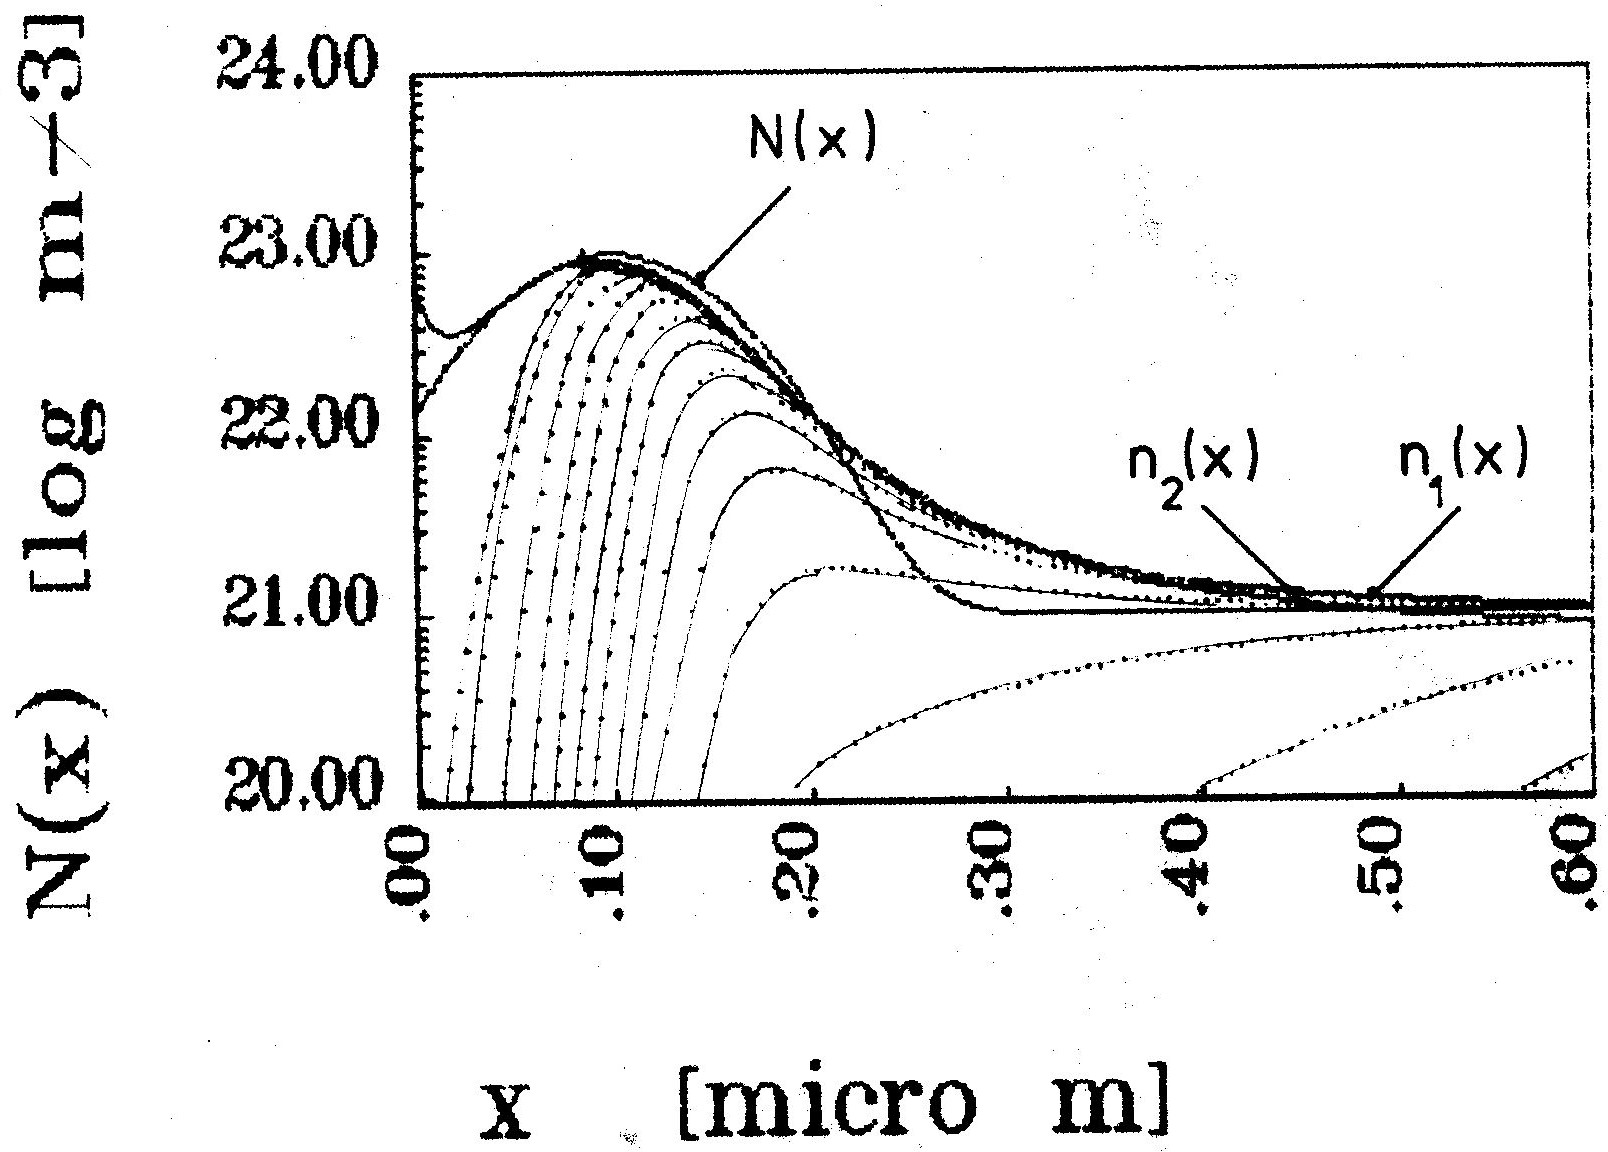
\includegraphics{Figures/fig-4-4.eps}
  \caption[Priebeh koncentrácie prímesí simulovaný Gaussovským
    rozložením]{Priebeh koncentrácie prímesí $N(x)$ simulovaný
    Gaussovským rozložením s parametrami $R_{p}=0.1\mu m$, $\Delta
    R_{p}=0.05\mu m$, $N_{\max}=1.0\times 10^{23} m^{-3}$,
    $N_{bulk}=1.0\times10^{21}m^{-3}$; priebeh majoritných nosičov
    náboja $n_{1}(x)$ a priebeh $n_{2}(x)$, získaný z teoretickej C-V
    závislosti. Bodkovanými čiarami je znázornené ochudobnovanie
    štruktúry MOS.}\label{fig:4.4}
\end{figure}
% OBR24.BIT

\begin{figure}[h!]\centering
  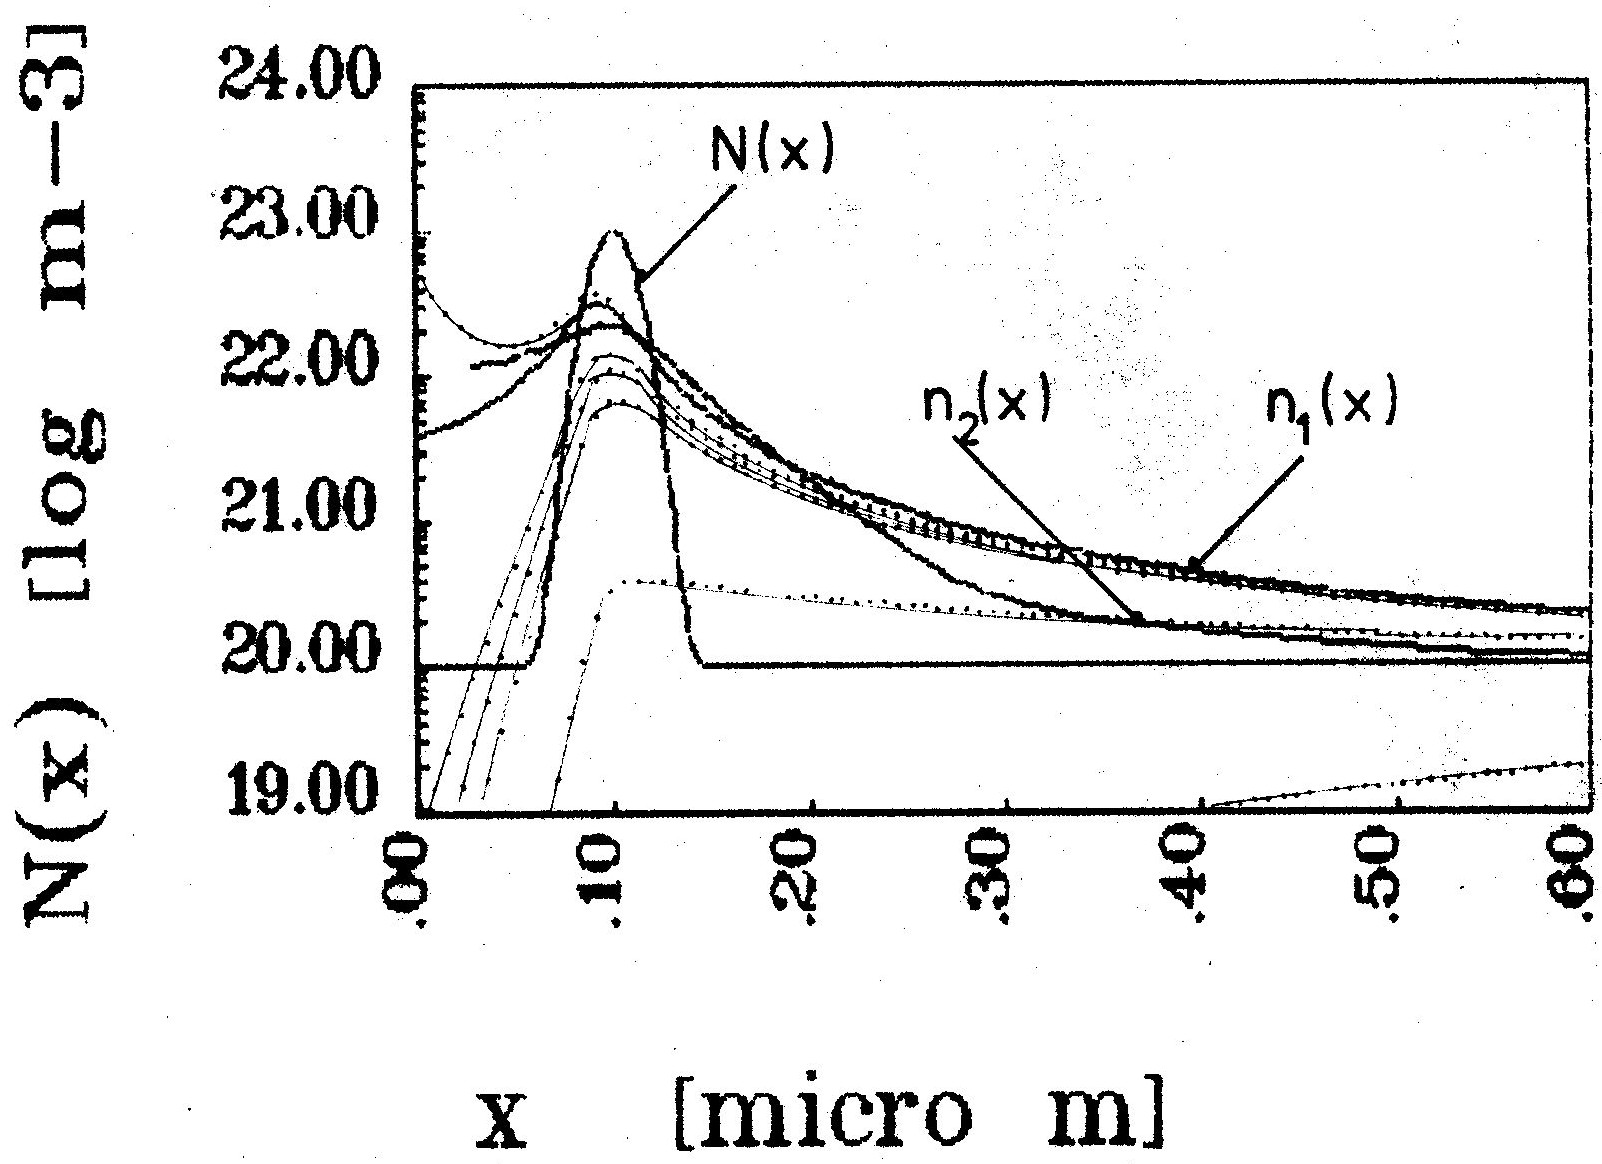
\includegraphics{Figures/fig-4-5.eps}
  \caption[Priebeh koncentrácie prímesí simulovaný Gaussovským
    rozložením]{Priebeh koncentrácie prímesí $N(x)$ simulovaný
    Gaussovským rozložením s parametrami $R_{p}=0.1\mu m$, $\Delta
    R_{p}=0.01\mu m$, $N_{\max}=1.0\times10^{23}m^{-3}$,
    $N_{bulk}=1.0\times10^{21}m^{-3}$; priebeh majoritných nosičov
    náboja $n_{1}(x)$ a priebeh $n_{2}(x)$, získaný z teoretickej C-V
    závislosti. Bodkovanými čiarami je znázornené ochudobnovanie
    štruktúry MOS.}\label{fig:4.5}
\end{figure}
%OBR25.BIT

\par Ďalšia analýza aproximácií, použitých pri výpočte koncentračných
profilov, by sa mohla zamerať na hľadanie exaktného obmedzenia
platnosti týchto aproximácií, avšak zo systematického hľadiska by bolo
pre riešenie tejto problematiky efektívnejšie zvoliť prístup, ku
ktorému sa vzťahuje následovná poznámka.

\par\emph{POZNÁMKA.} Pomocou kapacitných meraní by bolo možné určiť
priebeh $N(x)$ presne bez použitia aproximácií uvedených v
predchádzajúcich článkoch.  V práci~\cite{4.4} dodatku A je naznačený
postup výpočtu elektrického potenciálu v polovodiči, ktorý je funkciou
vzdialenosti (od povrchu polovodiča do hĺbky) a napätia hradla.
Deriváciou Poissonovej rovnice~\ref{eq:1.2} podľa $V_{g}$ dostávame
parciálnu diferenciálnu rovnicu tretieho rádu, ktorá presne opisuje
experiment merania C-V závislosti

\begin{equation}\label{eq:4.13}
  \frac{\delta^{3}\varphi}{\delta x^{2}\delta V_{g}} = {\frac{1}{L_{D}^{2}}}\ {e^{\beta\varphi}}\ {\frac{\delta\varphi}{\delta V_{g}}}
\end{equation}

Jej riešením použitím vhodných okrajových podmienok by bolo možné
získať plochu $\varphi(x,V_{g})$, z ktorej pre výpočet $N(x)$ je
potrebná len jedna priamka $\varphi(x)\rvert_{V_{g}}$

\begin{equation}\label{eq:4.14}
  N(x) = N_{bulk}\ e^{\beta\varphi}-\frac{\epsilon}{q}\frac{\delta^{2}\varphi}{\delta x^{2}}
\end{equation}

(todo: check equation 4.14 in ref 4.4)

Autori článku~\cite{4.4} túto metódu ďalej nerozvíjali, z dôvodov
ťažkosti pri vyčíslovani druhej derivácie vo vzorci~\ref{eq:4.14}.


\section{Určenie hustoty pascí rozhrania $Si-SiO_{2}$.}\label{sec:4.2}

Kvalitu rozhrania $Si-SiO_{2}$ charakterizujeme hustotou pascí
rozhrania $(D_{it})$, ktorá je dôsledkom mechanizmu termickej oxidácie
kremíka, pri ktorej dochádza k vytvoreniu oblasti s nestechiometrickým
zložením. Túto hustotu možno vyhodnotiť následujúcimi dvoma postupmi:

\begin{enumerate}
\item Porovnanie nameranej vysokofrekvenčnej C-V závislosti
  $C_{mos}^{HF}(V_{g})$ a nameranej nízkofrekvečnej C-V závislosti
  $C_{mos}^{LF}(V_{g})$. Vyhodnotenie $D_{it}$ pomocou porovnania
  uvedených závislostí vychádza z predpokladu, že závislosť
  $C_{mos}^{HF}(V_{g})$ je meraná dostatočne vysokým VF signálom, čo
  spôsobí, že kapacita nie je ovplyvnená pascami rozhrania
  $Si-SiO_{2}$.
\item Porovnanie nameranej závislosti $C_{mos}^{LF}(V_{g})$ a
  teoretickej nízkofrekvečnej C-V závislosti, ktorú označíme
  $C_{mos}^{TLF}(V_{g})$.  V tomto prípade je potrebné na základe
  známeho priebehu koncentračného profilu dotujúcich prímesí v
  podpovrchovej oblasti polovodiča vypočítať závislosť
  $C_{mos}^{TLF}(V_{g})$ riešením Poissonovej rovnice.
\end{enumerate}

Pre vyhodnotenie $D_{it}$ sme použili obe metódy, ktorých realizáciu v
ďalšom podrobne uvedieme.

\subsection{Porovnanie vysokofrekvenčnej a nízkofrekvenčnej C-V závislosti.}\label{sec:4.2.1}

V tomto prípade využijeme frekvenčnú závislost kapacity štruktúry MOS
a $D_{it}$ určíme z porovnania $C_{mos}^{HF}(V_{g})$ a
$C_{mos}^{LF}(V_{g})$. Potrebný teoretický základ možno nájsť
napríklad v~\cite{I.1}.  Pre určenie $C_{mos}^{HF}(V_{g})$ a
$C_{mos}^{LF}(V_{g})$ je vhodné použiť Q-C metódu~\cite{3.4, 3.6, 3.7,
  3.8}, ktorá umožňuje simultánne určenie oboch závislostí, avšak
použitie štandardných metód určovania $C_{mos}^{HF}(V_{g})$ a
$C_{mos}^{LF}(V_{g})$ je tiež možné.

\begin{figure}[h!]\centering
  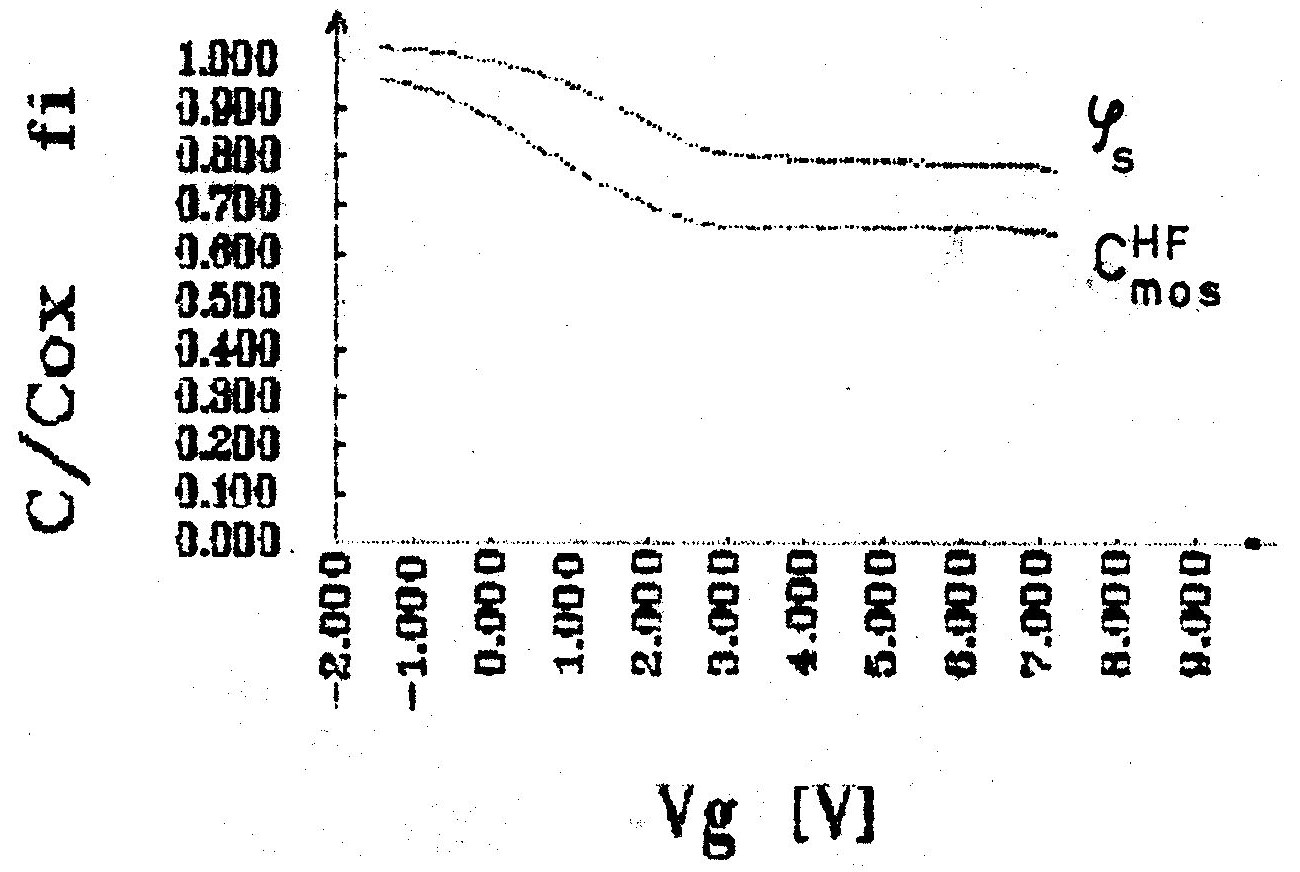
\includegraphics{Figures/fig-4-6.eps}
  \caption[VF C-V závislosť $C_{mos}^{HF}(V_{g})$ a priebeh
    povrchového potenciálu $\varphi_{s}(V_{g})$ štruktúry MOS získané
    pomocou Q-C metódy]{VF C-V závislosť $C_{mos}^{HF}(V_{g})$
    normovaná na kapacitu oxidu a normovaný priebeh povrchového
    potenciálu $\varphi_{s}(V_{g})$ štruktúry MOS získané pomocou Q-C
    metódy.  Priebeh povrchového potenciálu je normovaný vzťahom
    $1-\frac{\varphi_{s}}{\varphi_{norm}}$, kde
    $\varphi_{norm}=3.33$.}\label{fig:4.6}
\end{figure}
% OBR15.BIT

Na obrázku~\ref{fig:4.6} sú namerané hodnoty $C_{mos}^{HF}(V_{g})$ a
povrchového potenciálu $\varphi_{s}$ štruktúry MOS, určené pomocou Q-C
metódy. Na obrázku~\ref{fig:4.7} sa nachádzajú krivky
$C_{mos}^{HF}(V_{g})$ a $C_{mos}^{LF}(V_{g})$, ktoré použijeme pre
výpočet $D_{it}$ podľa následujúceho vzťahu~\cite{4.15}

\begin{equation}\label{eq:4.15}
  D_{it} = {\frac{1}{q}} {\left[\frac{C_{mos}^{LF}}{1-\frac{C_{mos}^{LF}}{C_{ox}}}-\frac{C_{mos}^{HF}}{1-\frac{C_{mos}^{HF}}{C_{ox}}}\right]}
\end{equation}
% was (4.14) in origin

\begin{figure}[h!]\centering
  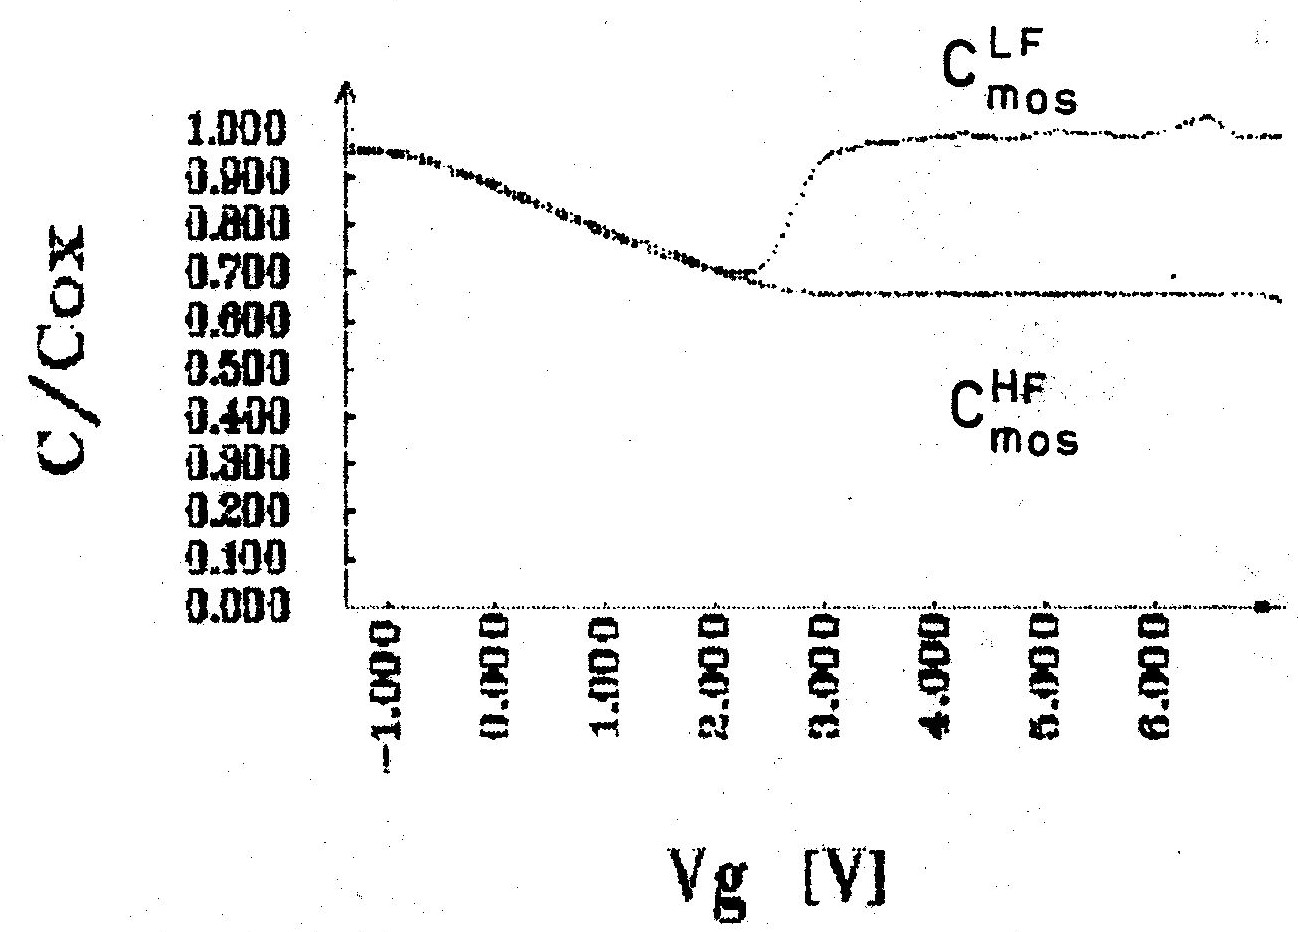
\includegraphics{Figures/fig-4-7.eps}
  \caption[VF C-V závislosť $C_{mos}^{HF}(V_{g})$ a LF C-V závislosť
    $C_{mos}^{LF}(V_{g})$ štruktúry MOS normované na kapacitu oxidu,
    získané pomocou Q-C metódy]{VF C-V závislosť $C_{mos}^{HF}(V_{g})$
    a LF C-V závislosť $C_{mos}^{LF}(V_{g})$ štruktúry MOS normované
    na kapacitu oxidu, získané pomocou Q-C metódy.  LF C-V závislosť
    je vypočítaná deriváciou povrchového potenciálu (zobrazeného na
    obrázku~\ref{fig:4.6}) podľa vzťahu~\ref{eq:3.2}.}\label{fig:4.7}
\end{figure}
% OBR12.BIT

\par Polohu Fermiho hladiny v zakázanom pásme pre vypočítané hodnoty
$D_{it}$ určíme pomocou hodnôt povrchového potenciálu $\varphi_{s}$ a
vzdialenosti Fermiho hladiny od intrinzickej Fermiho hladiny
$\varphi_{f}$. Priebeh povrchového potenciálu $\varphi_{s}(V_{g})$
získame buď priamo pomocou Q-C metódy, alebo integráciou
kvázistatickej C-V závislosti použitím Berglundovho integrálu. V oboch
prípadoch dostávame priebehy $\varphi_{s}(V_{g})$, ktoré sú posunuté v
smere osi $y$. V prípade Q-C metódy sa jedná o konštantu
$\varphi_{s0}$, ktorá predstavuje povrchový potenciál, ak na hradle
štruktúry MOS nie je pripojené napätie a v prípade kvázistatickej C-V
metódy posunutie predstavuje integračnú konštantu. Pre obidva prípady
môžeme posunutie závislosti $\varphi_{s}(V_{g})$ vypočítať postupom
uvedeným v dodatku~\ref{app:AppendixG}.

\begin{figure}[h!]\centering
  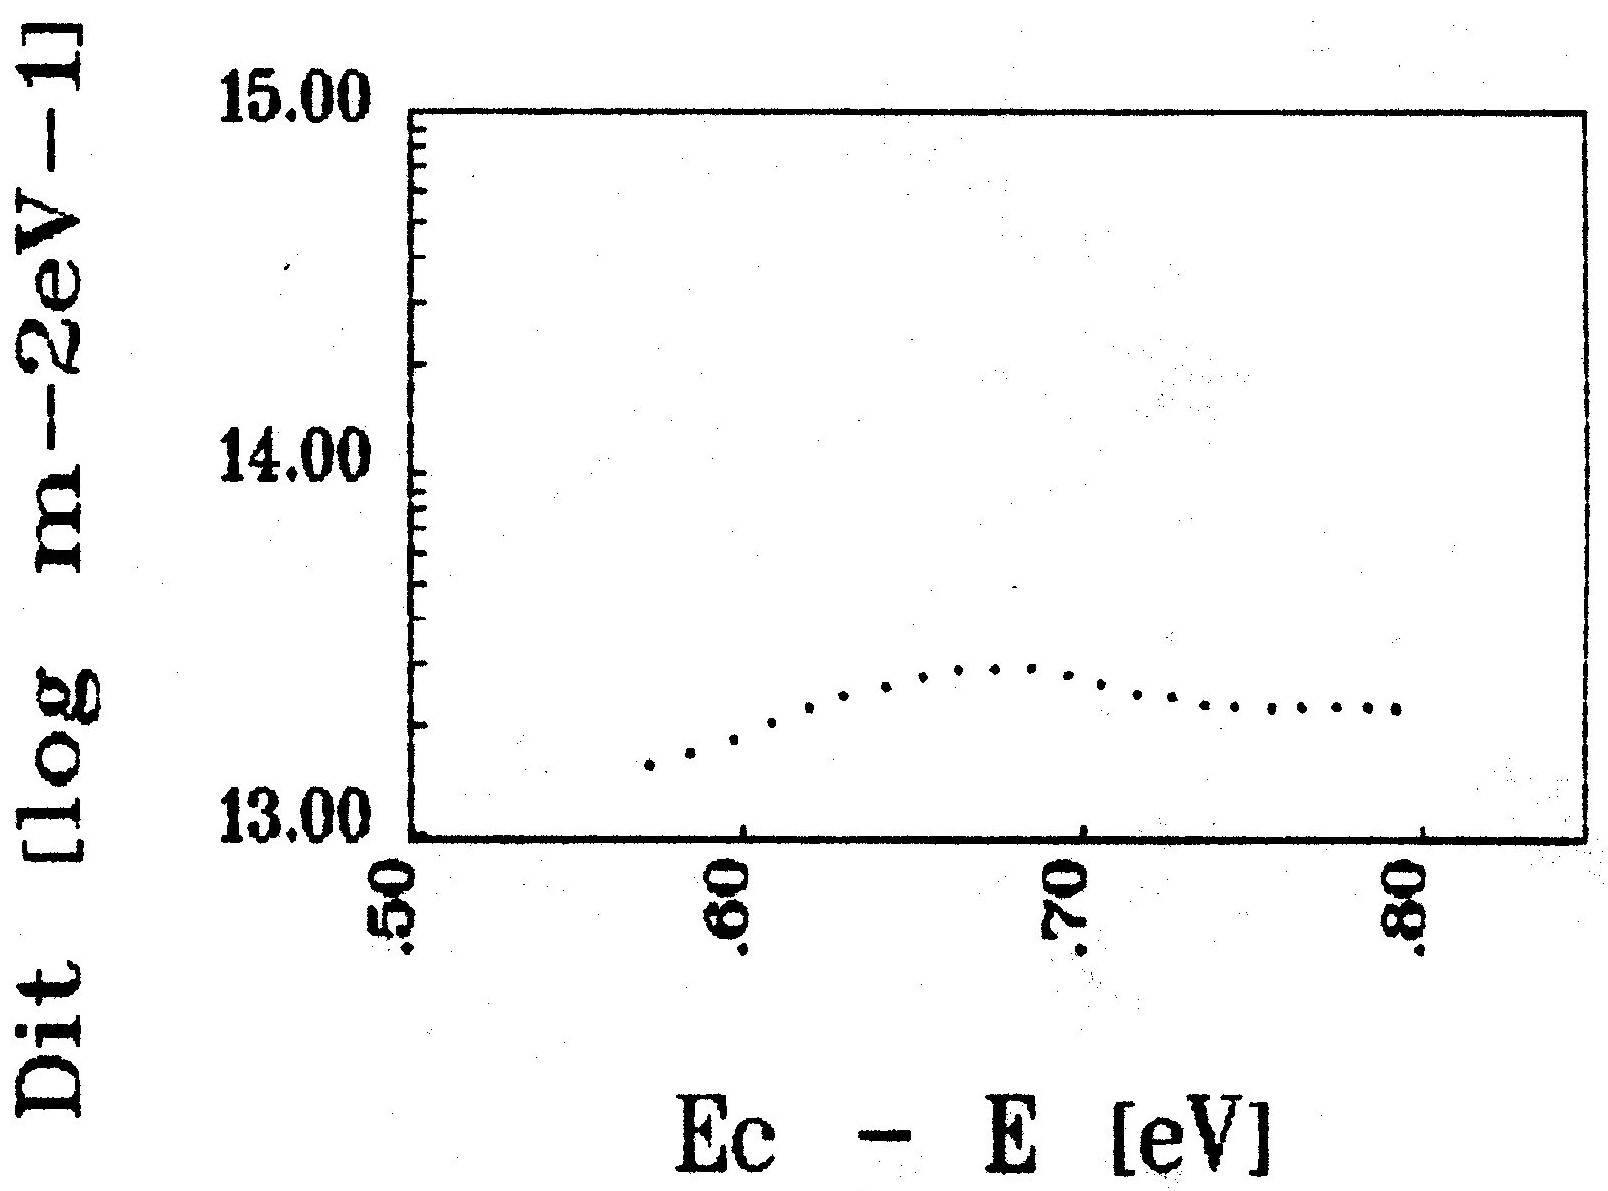
\includegraphics{Figures/fig-4-8.eps}
  \caption[Závislosť $D_{it}$ od polohy v zakázanom pásme polovodiča
    typu P, určená z porovnania $C_{mos}^{HF}(V_{g})$ a
    $C_{mos}^{LF}(V_{g})$]{Závislosť $D_{it}$ od polohy v zakázanom
    pásme polovodiča typu P, určená z porovnania $C_{mos}^{HF}(V_{g})$
    a $C_{mos}^{LF}(V_{g})$, ktoré sú zobrazené na
    obrázku~\ref{fig:4.7}.}\label{fig:4.8}
\end{figure}
% OBR14.BIT

Hodnotu potenciálu $\varphi_{f}$ určíme pomocou vzťahu

\begin{equation}\label{eq:4.16}
  \varphi_{f} = \pm \frac{kT}{g} \ln{\frac{N_{b}}{n_{i}}}
\end{equation}

, kde predpokladáme znalosť koncentrácie substrátu $N_{b}$. Potenciál
$\varphi_{f}$ má kladné znamienko pre polovodič typu P. Ak pre
povrchový potenciál $\varphi_{s}$ zvolíme tú istú orientáciu ako pre
potenciál $\varphi_{f}$, energetickú polohu pascí rozhrania v
zakázanom pásme potom určíme pomocou následovného vzťahu

\begin{equation}\label{eq:4.17}
  E_{c} - E = 0.56 + \varphi_{s} + \varphi_{f}
\end{equation}

,kde číslo $0.56$ predstavuje vzdialenosť dolného okraja vodivostného
pásma $(E_{c})$ od intrinzickej Fermiho hladiny. Priebeh $D_{it}$ ako
funkcie polohy v zakázanom pásme je znázornený na
obrázku~\ref{fig:4.8}.


\subsection{Porovnanie experimentálnej a teoretickej kvázistatickej CV závislosti.}\label{sec:4.2.2}

Pre výpočet $D_{it}$ pomocou tejto metódy je potrebné poznať priebeh
koncentračného profilu dotujúcich prímesí v podpovrchovej oblasti
polovodiča $N(x)$, aby sme mohli vypočítať
$C_{mos}^{TLF}(V_{g})$. Teoretickú závislosť $C_{mos}^{TLF}(V_{g})$
štruktúry MOS vypočítame numerickým postupom popísaným v
dodatku~\ref{app:AppendixA}.  Použitie numerických metód je v tomto
prípade nevyhnutné, pretože analytické riešenie Poissonovej rovnice
nie je možné pre všeobecný priebeh koncentrácie $N(x)$.  Pri
numerickom riešení Poissonovej rovnice zároveň vypočítame závislosť
povrchového potenciálu od napätia hradla $\varphi_{s}(V_{g})$, ktorú
použijeme pre určenie pozície vypočítanej hustoty pascí rozhrania v
zakázanom pásme polovodiča.  Pretože počas numerického výpočtu
neberieme do úvahy poruchové náboje v oxidovej vrstve a na rozhraní
$Si-SiO_{2}$ obidve teoreticky určené závislosti $\varphi_{s}(V_{g})$
aj $C_{mos}^{TLF}(V_{g})$ budú posunuté voči nameranej kvázistatickej
C-V závislosti o hodnotu $V_{FB}$. Pre posunutie uvedených závislostí
musíme poznať aj hodnotu $V_{FB}$.

\par Pre výpočet $D_{it}$ teda použijeme $C_{mos}^{TLF}(V_{g})$, ktorá
nie je zaťažená kapacitou pascí rozhrania $Si-SiO_{2}$. Na
obrázku~\ref{fig:4.9} sú zobrazené nameraná a teoretická LF C-V
závislosť, ktoré ďalej použijeme na vyhodnotenie $D_{it}$ podľa vzťahu

\begin{equation}\label{eq:4.18}
  D_{it} = \frac{1}{q} \left[\cfrac{C_{mos}^{LF}}{1-\cfrac{C_{mos}^{LF}}{C_{ox}}}-\cfrac{C_{mos}^{TLF}}{1-\cfrac{C_{mos}^{TLF}}{C_{ox}}}\right]
\end{equation}
% was (4.15) in origin (as an error of copying

Na obrázku~\ref{fig:4.10} je znázornený priebeh hustoty pascí
rozhrania v závislosti od polohy v zakázanom pásme polovodiča určený
uvedeným spôsobom.  Nevýhoda popísanej metódy spočíva v časovej
náročnosti výpočtu teoretickej nízkofrekvenčnej C-V
závislosti. Napriek tomu, že porovnanie teoretickej a experimentálnej
nízkofrekvenčnej C-V závislosti poskytuje hodnoty$D_{it}$ vo väčšej
oblasti zakázaného pásma, pre vyhodnocovanie plošného rozloženia
$D_{it}$ na kremíkovej doske sme z časových dôvodov použili postup
popísaný v časti~\ref{sec:4.2.1}

\begin{figure}[h!]\centering
  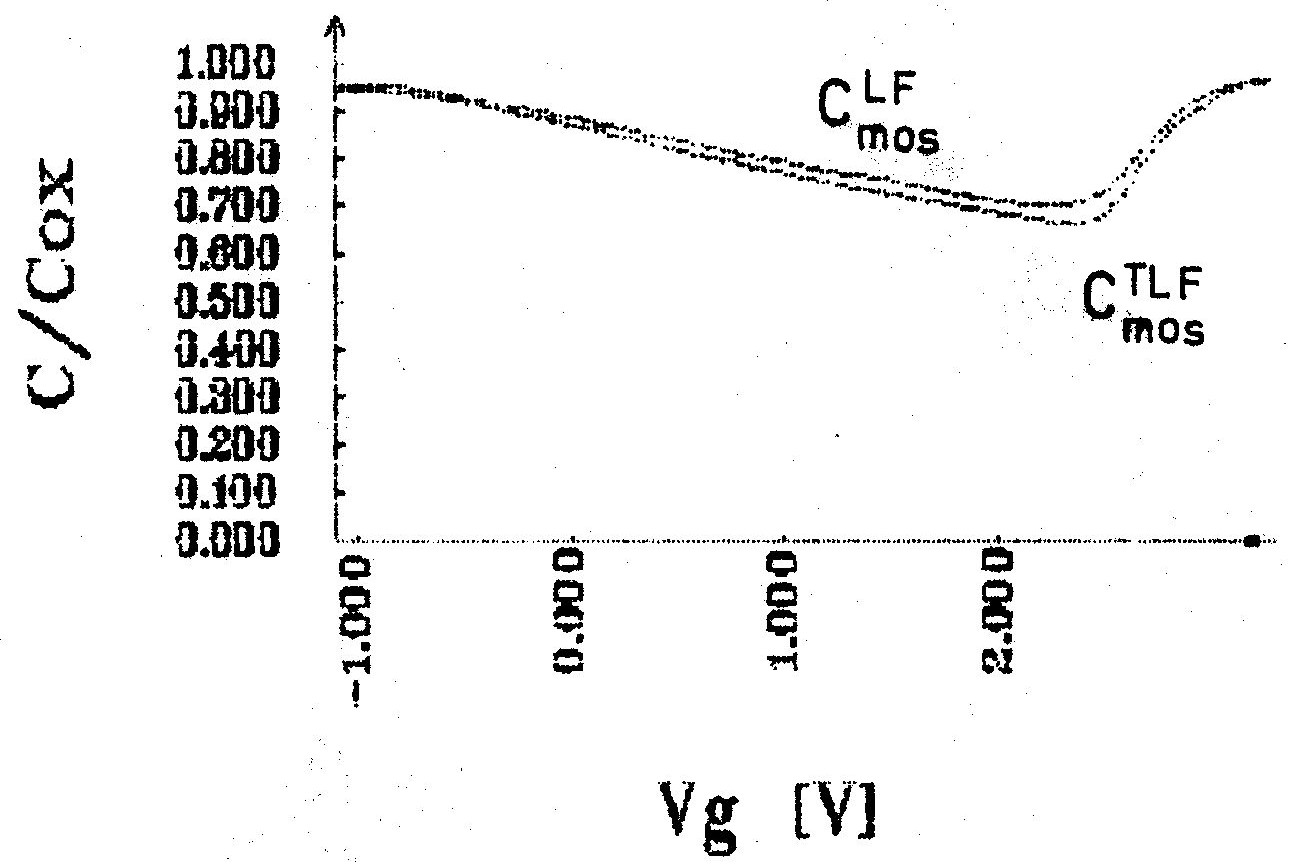
\includegraphics{Figures/fig-4-9.eps}
  \caption[Teoretická LF C-V závislosť a nameraná LF C-V
    závislosť]{Teoretická LF C-V závislosť a nameraná LF C-V závislosť
    štruktúry MOS normované na kapacitu oxidu.}\label{fig:4.9}
\end{figure}
% OBR11.BIT

\begin{figure}[h!]\centering
  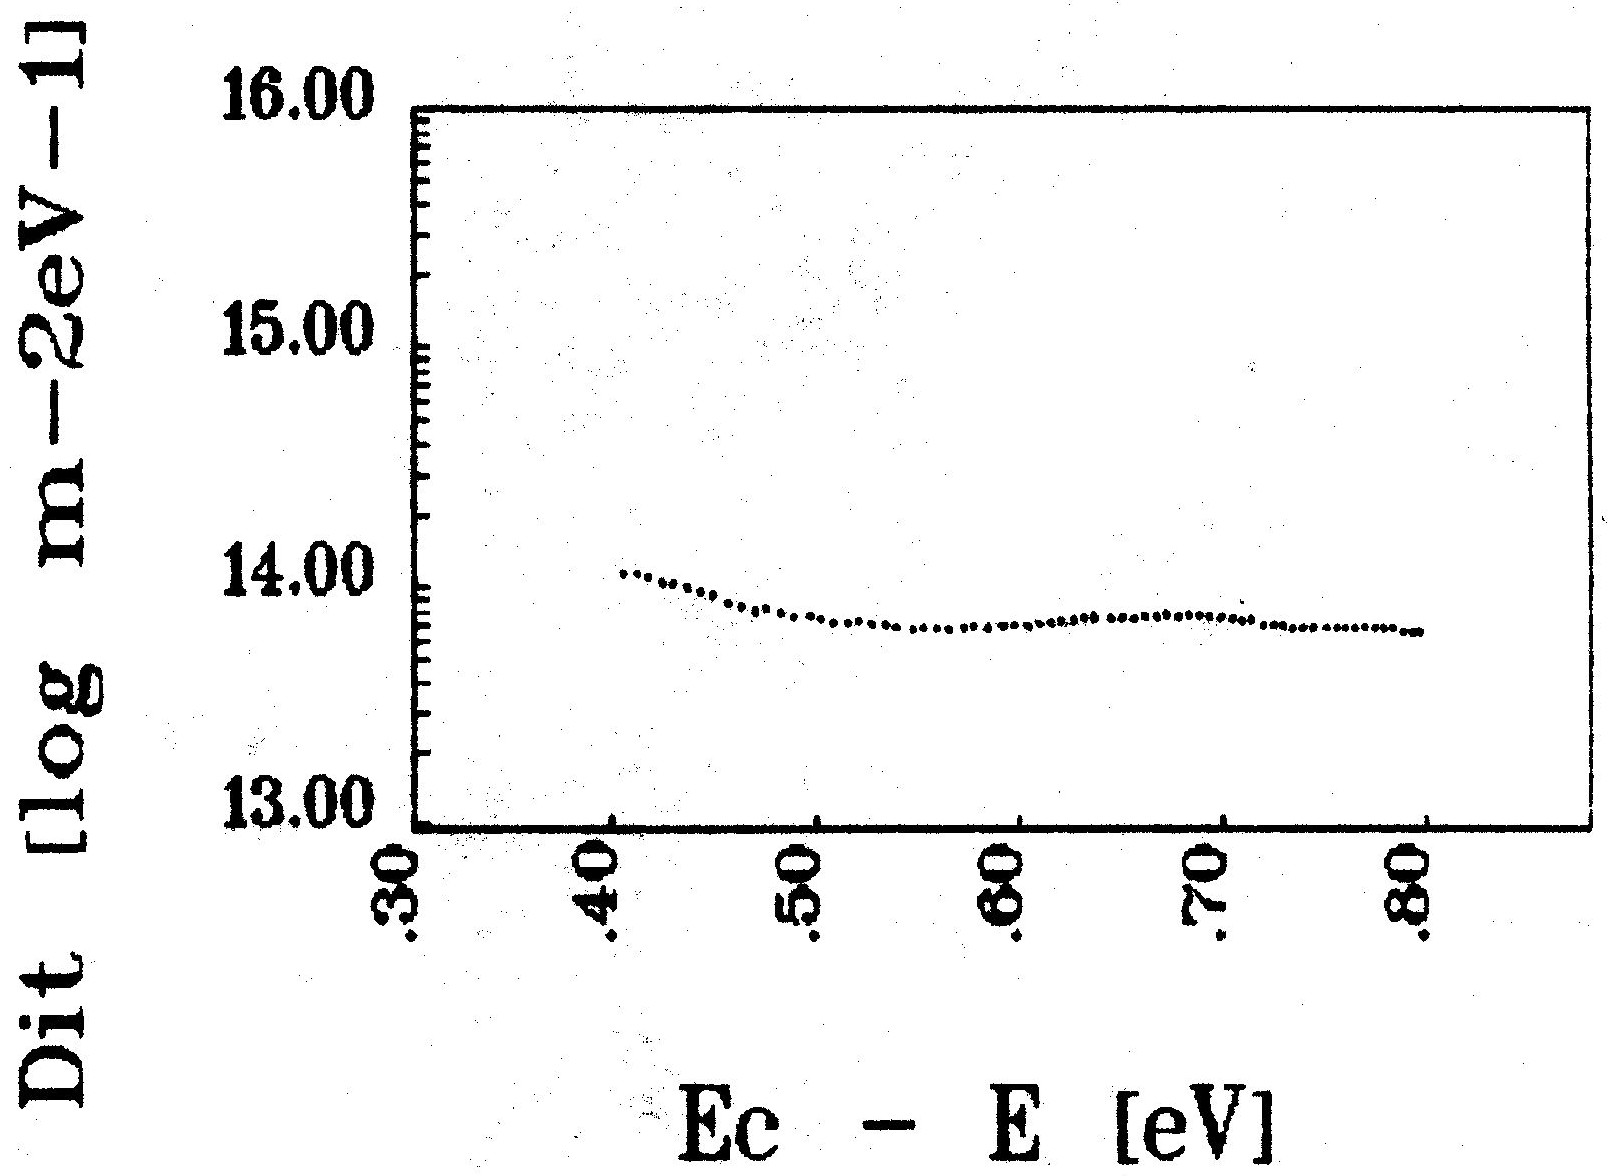
\includegraphics{Figures/fig-4-10.eps}
  \caption[Závislosť $D_{it}$ od polohy v zakázanom pásme polovodiča
    určená z porovnania $C_{mos}^{TLF}(V_{g})$ a
    $C_{mos}^{LF}(V_{g})$]{Závislosť $D_{it}$ od polohy v zakázanom
    pásme polovodiča typu P, určená z porovnania
    $C_{mos}^{TLF}(V_{g})$ a $C_{mos}^{LF}(V_{g})$, ktoré sú zobrazené
    na obrázku~\ref{fig:4.9}.}\label{fig:4.10}
\end{figure}
% OBR13.BIT


\begin{thebibliography}{}
\bibitem[4.1]{4.1} Lehovec K.: Solid St\.  Electron.  27 (1984)
  s.1907.
\bibitem[4.2]{4.2} Wu Chung P., Douglas E.C., Mueller C.W.: IEEE
  Trans.\ on elektron.\ dev. 22 (1975) s.319.
\bibitem[4.3]{4.3} Kroemer H., Chien W.: Solid St.\ Electron. 24
  (1981) s.655.
\bibitem[4.4]{4.4} Baccarani G., Rudan M., Maes H., Vandervorst W.,
  Van Overstraeten R.: Solid St\. Electron. 23 (1980) s. 65.
\bibitem[4.5]{4.5} Botka V., Csabay O., Artz P., Beyer A.: 3.vedecká
  konferencia EF SVŠT Elektrotechnika '90, EF SVŠT Bratislava, 1990
  s.73.
\bibitem[4.6]{4.6} Kinder R.: Príspevok ku skúmaniu koncentračných
  profilov implantovaných vrstiev. Kandidátska dizertačná práca. EF
  SVŠT Bratislava 1984.
\bibitem[4.7]{4.7} Lin S.T., Reuter J.: Solid St.\ Electron. 26 (1983)
  s.343.
\bibitem[4.8]{4.8} Ziegler K., Klausmann E.: Solid St.\ Electron. 18
  (1975) s.189.
\bibitem[4.9]{4.9} Jindal R.P., Warner R.M. Jr.: IEEE Trans.\ on
  elektron.\ dev. 28 (1981) s.348.
\bibitem[4.10]{4.10} Jindal R.P.: Solid St.\ Electron. 26 (1983)
  s.1005.
\bibitem[4.11]{4.11} Warner R.M. Jr., Jindal R.P.: Solid
  St.\ Electron. 26 (1983) s.335.
\bibitem[4.12]{4.12} Balland B., Remaki B., Marchand J.J.:
  J. Phys. E. Sci. Instrum. 21 (1988) s.559.
\bibitem[4.13]{4.13} Csabay O., Botka V.: 5.celoštátna konferencia
  Mikroelektronika 1989, Dom techniky ČSVTS Bratislava, 1989 s.58.
\bibitem[4.14]{4.14} Zsalkovics G.: Určovanie koncentračného profilu
  implantovanej vrstvy z kapacitných meraní. Diplomová práca, Katedra
  mikroelektroniky, EF SVŠT, Bratislava 1988.
\bibitem[4.15]{4.15} Zohta Y.: Solid St.\ Electron. 17 (1974), s.1299.
\bibitem[4.16]{4.16} Kennedy O.P., Murley P.C., Kleinfelder W.: IBM
  J. Res. Dev. 12 (1968) s.399.
\bibitem[4.17]{4.17} Nishida V.: IEEE Trans. Electron. Dev. ED-26
  (1979) s.1081.
\bibitem[4.18]{4.18} Johnson W.C., Panousis P.T.: IEEE
  Trans. Electron. Dev. ED-18 (1971) s.965.
\bibitem[4.19]{4.19} Isaacson E., Keller H.B.: Analysis of numerical
  memethods.  John Wiley and Sons. New York.
\bibitem[4.20]{4.20} Vitásek E.: Numerické metody. SNTL, Praha 1987.
\bibitem[4.21]{4.21} Hamming R.W.: Digital filters. Prentice Hall.
\bibitem[4.22]{4.22} Beyer A., Tolonics J.: Physik der
  Halbleiteroberflbche 17 (1986) s.91.
\end{thebibliography}
 
% Chapter 5

\chapter{Pracovisko pre automatizovaný zber dát.}\label{Chapter5}
\lhead{Kapitola 5. \emph{Pracovisko pre automatizovaný zber dát}}

Na popisovanom pracovisku možno automaticky merať vysokofrekvenčnú a
nízkofrekvenčnú kapacitu štruktúry MOS\@. Na obrázku~\ref{fig:5.1} je
zobrazené blokové zapojenie prístrojov, pomocou ktorých sú jednotlivé
metódy realizované.

\begin{figure}[h!]\centering
  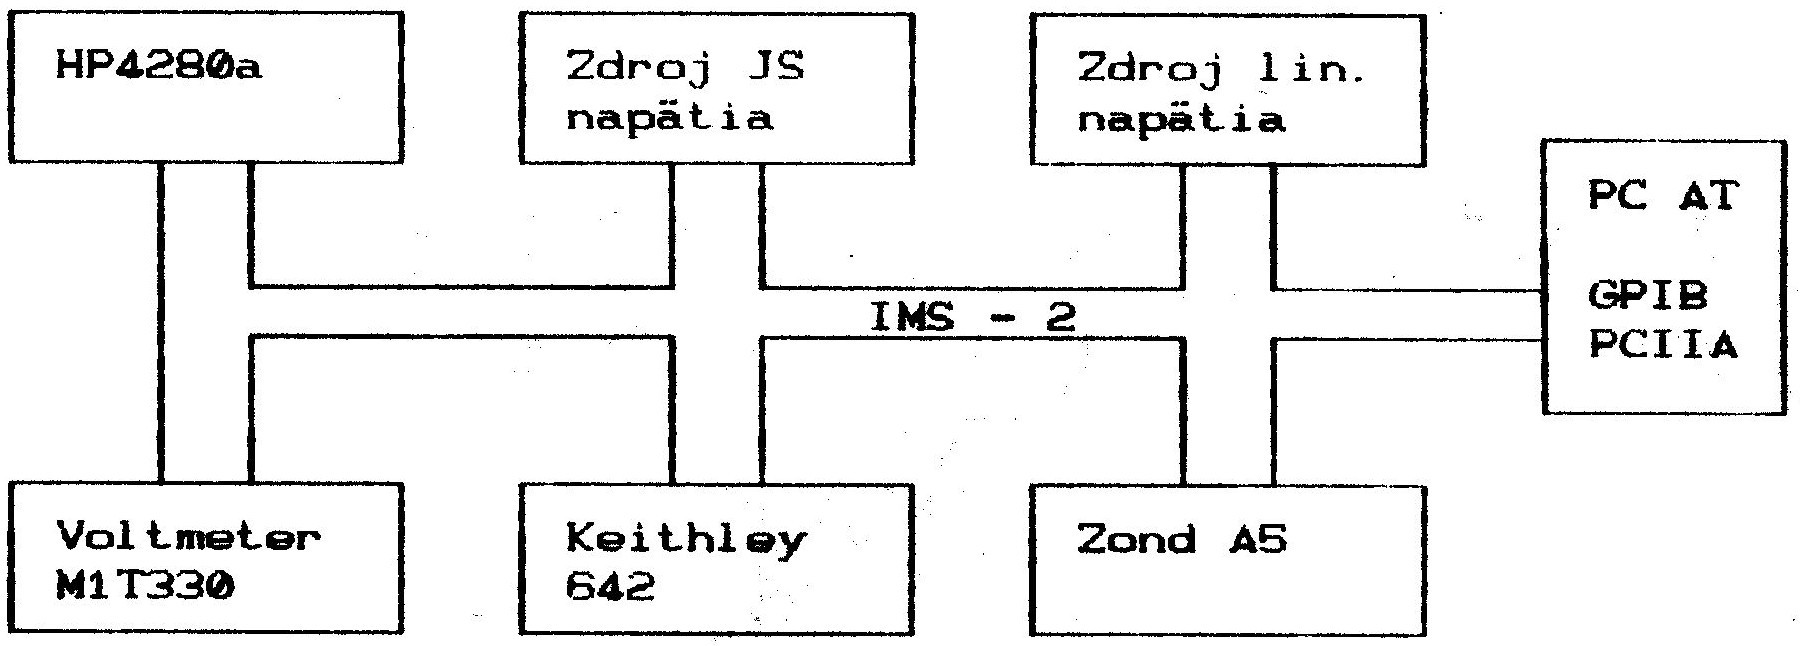
\includegraphics{Figures/fig-5-1.eps}% chktex-file 8
  \caption[Bloková schéma zapojenia prístrojov automatizovaného
    pracoviska]{Bloková schéma zapojenia prístrojov automatizovaného
    pracoviska pre určovanie plošného rozloženia parametrov štruktúr
    MOS s nehomogénnou dotáciou substrátu.}\label{fig:5.1}
\end{figure}

Riadiacim počítačom meraní je osobný počítač PC AT vybavený
interfejsom IMS-2 (norma IEEE 488) firmy National Instruments model
GPIB-PCIIA, ktorý pracuje ako radič zbernice IMS-2. Všetky pripojené
prístroje sú vybavené interfejsom IMS-2, pomocou ktorého ich možno
diaľkovo ovládať a zberať namerané údaje. Okrem profesionálnych
meracích prístrojov HP4280a a Keithley 642 boli v experimente použité
zdroje jednosmerného napätia a zdroj lineárne narastajúceho napätia
postavené na Katedre mikroelektroniky. Voltmeter M1T330 je výrobkom
Metry Blansko a krokovacie hrotové zariadenie Zond A5 bolo dovezené zo
Sovietskeho Zväzu. Posledne spomínané zariadenie neobsahuje štandardne
interfejs IMS-2 a bolo dodatočne vybavené modulom IMS-2 vlastnej
konštrukcie~\cite{5.1}.

Ďalším novým prvkom našej realizácie pracoviska pre meranie štruktúr
MOS je možnosť automatického zberu dát po celej kremíkovej doske a ich
uloženie do diskového súboru pre následovné spracovanie. Programové
vybavenie pracoviska možno rozdeliť na programy (1) zberu dát (2)
spracovania dát (3) zobrazenia výsledkov a (4) pomocné
programy. Programy zberu dát umožňujú meranie C-V závislosti v
ľubovoľnom počte bodov kremíkovej dosky, ktorých pozície sú voliteľné
a sú definované operátorom.

Dôležitým momentom pri realizácii programov zberu dát bolo
zabezpečenie proti strate nameraných dát v dôsledku výskytu ľubovolnej
chyby (napr.\ výpadku napätia), alebo v prípade nutnosti prerušiť
meranie. Pretože trvanie zberu dát na kremíkovej doske s 300
štruktúrami sa pohybuje od 0.5 do 12 hodín v závislosti od
požadovaného druhu merania, bolo potrebné programovo zabezpečiť (1)
možnosť prerušenia merania operátorom v ľubovoľnom bode (2) možnosť
opätovného reštartovania zberu dát v bode, kde bol zber dát
prerušený. Zabezpečenie uchovania nameraných dát v prípade výskytu
chyby bolo realizované nasledovným spôsobom. Namerané dáta sú naraz
zapisované do diskového súboru vždy po ukončení merania na každej
štruktúre. Túto dátovú jednotku budeme v ďalšom označovať záznam. To
znamená, že k poškodeniu štruktúry dát môže prísť len v prípade
výskytu chyby v priebehu krátkeho časového úseku (rádove desiatky ms),
čím ale prichádza len k strate posledného záznamu. Pre tento prípad je
k dispozícii pomocný program, ktorý skráti dátový súbor na požadované
množstvo záznamov, čím obnoví kompaktnosť súboru a umožní
reštartovanie zberu dát. Týmto spôsobom možno skrátiť dátový súbor o
chybne namerané dáta aj po prerušení zberu dát operátorom, ak bola
zistená nejaká závada v priebehu merania. Zároveň je k dispozícii
pomocný program, ktorý umožňuje prepísanie ľubovolného počtu záznamov
dátového súboru. Užitočnosť tohto programu vysvetlíme v nasledovnom
príklade.

Predstavme si, že v priebehu zberu dát došlo (napr.dôsledkom vplyvov
okolia) ku chybe, ktorá trvala krátky časový úsek, čo spôsobilo, že
časť záznamov dátového súboru obsahuje chybné dáta. Príkladom môže byť
nedokonalosť kontaktu hrotu s meranou vzorkou spôsobená vibráciami. To
sa často zistí až pri vyhodnocovaní merania, prípadne pri zobrazení
výsledkov. Po určení pozícií štruktúr na testovanej kremíkovej doske,
v ktorých sme namerali chybné údaje, môžeme v týchto bodoch meranie
zopakovať a pomocným programom prepísať záznamy v pôvodnom dátovom
súbore.

Uvedeným spôsobom boli realizované programy zberu dát pre HF C-V,
kvázistatickú C-V metódu, meranie kapacity oxidovej vrstvy a metódu
konštantnej šírky oblasti priestorového náboja. Takto sme ale nemohli
automatizovať Q-C metódu, pretože použitý interfejs prístroja Keithley
642 neumožňuje diaľkové ovládanie zkratovania vstupných svoriek
meracieho prístroja, čím nemožno automatizovať vynulovanie náboja v
spoločnom bode zapojenia kondenzátorov, ktorý sa tam dostane vplyvom
zvodových prúdov.

Pre pohodlnú manipuláciu s dátovými súbormi bola zvolená nasledovná
koncepcia pomenovania dátových súborov. Pomenovanie súboru v operačnom
systéme MS DOS pozostáva z mena súboru a prípony.  Meno súboru
predstavuje v našom prípade názov meranej kremíkovej dosky a prípona
označuje druh dát, ktoré súbor obsahuje. Principiálne možno rozdeliť
uvedené dátové súbory na dva typy podľa dát, ktoré obsahujú jednotlivé
záznamy. Môže to byť funkčná závislosť alebo parameter. Ak sa jedná o
funkčnú závislosť, potom prvý záznam v dátovom súbore obsahuje počet
bodov, v ktorých bola funkčná závislosť zosnímaná a hodnoty nezávislej
premennej. Ďalšie záznamy obsahujú pozíciu štruktúry na kremíkovej
doske, vyjadrenú dvoma celými číslami (X,Y), počet bodov a funkčné
hodnoty.  Opakujúca sa informácia o počte bodov funkčnej závislosti
nie je redundantná, pretože v prípade neúspešnosti merania
(napr.prieraz) na štruktúre (X,Y) obsahuje číslo -1, ktoré oznamuje
neprítomnosť funkčných hodnôt v zázname. Príkladom môže byť HF C-V
závislosť. Prvý záznam obsahuje počet meraní kapacity na jednej
štruktúre a hodnoty napätia hradla. Ďalšie záznamy obsahujú pozíciu
štruktúry (X,Y), počet bodov a hodnoty kapacity zodpovedajúce
hradlovým napätiam z prvého záznamu. Súbory druhého typu pozostávajú
len zo záznamov, ktoré obsahujú pozície štruktúry (X,Y) a hodnotu
parametra. Ako príklad uvedieme dátový súbor, ktorý obsahuje kapacity
oxidovej vrstvy štruktúr MOS\@. Pretože sa jedná o rozsiahle dátové
súbory bola zvolená binárna forma záznamu.  Celočíselné hodnoty majú
dĺžku 2 bajty a čísla s pohyblivou desatinnou čiarkou zaberajú 4
bajty.

Pre prípad, že by bol potrebný dátový súbor, obsahujúci dáta vo forme
ASCII, je k dispozícii pomocný program, ktorý po zadaní pozície
štruktúry (X,Y) vytvorí tento dátový súbor a zapíše do neho dáta,
ktoré obsahuje záznam s pozíciou (X,Y). Ak sa jedná o funkčnú
závislosť, zapíše do výstupného súboru vo forme ASCII aj hodnoty
nezávislej premennej.

\section{Meranie HF C-V závislostí.}\label{sec:5.1}

HF C-V závislosť štruktúry MOS meriame pomocou prístroja HP4280a,
ktorý určuje zároveň kapacitu a vodivosť meranej vzorky na základe
fázového posunu medzi HF napäťovým signálom (1MHz,30mV) a meraným
prúdom. Prístroj HP4280a je vybavený vlastným procesorom, ktorý riadi
jeho vnútorné funkcie a operátorovi poskytuje komfortné ovládanie. Pre
meranie HF C-V závislosti musíme nastaviť požadovaný interval napätia,
v ktorom sa má merať kapacita ($V_{start}$, $V_{stop}$) a napäťový
krok $V_{step}$, ktorým sa bude jednosmerné napätie meniť. Časové
pomery merania sa určujú ďalšími dvoma parametrami. $T_{hold}$ určuje
čas, počas ktorého bude na meranej vzorke pripojené napätie
$V_{start}$ pred začiatkom merania. Tento čas je potrebný na ustálenie
prechodových javov, v prípade že ich nechceme merať. Parameter
$T_{delay}$ určuje dobu pozdržania merania po vykonaní napäťového
  kroku.

Pre automatizované meranie štruktúr sme zvolili najvýkonnejší mód
prístroja HP4280a, v ktorom podľa vopred nastavených parametrov
automaticky vykoná celé meranie a namerané dáta uloží do vnútornej
pamäte.  Prenos dát z prístroja HP4280a do riadiaceho počítača sa
vykoná v binárnej forme, čím nestrácame čas konverziou medzi binárnou
formou a formou ASCII a zároveň binárna forma predstavuje menšie
množstvo prenášaných bajtov. Ukončenie merania a pripravenosť na
prenos dát signalizuje prístroj HP4280a nastavením signálu SRQ
(Service Request) na zbernici IMS-2, čím je synchronizovaná jeho
činnosť s riadiacim počítačom.  Tu možno spomenúť užitočnú vlastnosť
interfejsu GPIB-PCIIA~\cite{5.2}, ktorý po detekovaní signálu SRQ môže
automaticky vykonať sériové hlásenie prístrojov (Serial Poll) a po
nájdení prístroja, ktorý žiada o obsluhu uložiť jeho stavové slovo do
internej pamäte. Tým je vodič SRQ zbernice IMS-2 uvoľnený a interfejs
GPIB-PCIIA môže reagovať na žiadosť o obsluhu od ďalších
prístrojov. Ak riadiaci program požaduje stavové slovo prístroja,
ktorý žiadal o obsluhu, interfejs GPIB-PCIIA ho vydá zo svojej
internej pamäte.

Použitím automatického riadenia merania a binárneho prenosu dát sa
podarilo dosiahnuť minimálny čas HF C-V merania.  Konkrétne hodnoty
trvania meraní a časové diagramy sú v časti~\ref{sec:5.4}.

Ak potrebujeme určiť koncentračný profil dotujúcich prímesí vo väčšej
hĺbke, ako je šírka OPN v stave inverzie, musíme zmerať C-V závislosť
v stave hlbokého ochudobnenia. V tomto prípade sa vždy po napäťovom
skoku do stavu hlbokého ochudobnenia (a zmerania kapacity) musíme
vrátiť na určitý čas do stavu akumulácie. Prístroj HP4280a nemá mód
činnosti, ktorý by automaticky riadil tento druh merania. Preto musíme
každé meranie kapacity riadiť samostatne. Merací cyklus riadiaceho
programu potom obsahuje nastavenie požadovaného hradlového napätia,
prevedenie merania kapacity (spustenie merania a čakanie na jeho
ukončenie) a prenos dát z meracieho prístroja do riadiaceho počítača,
pričom všetky uvedené prenosy sa vykonávajú vo forme ASCII\@. Oproti
štandardnej HF C-V metóde sa dĺžka merania jedného bodu C-V závislosti
o rád zväčší.

Presnosť určenia koncentračného profilu dotujúcich prímesí silne
závisí od presnosti určenia kapacity oxidovej vrstvy.  Preto je
kapacita oxidu určovaná pomocou samostatného programu, ktorý meria
kapacitu štruktúry MOS pre zadané hradlové napätie ďaleko v akumulácii
a namerané hodnoty uloží do samostatného dátového súboru.

\section{Meranie kvázistatických C-V závislostí.}\label{sec:5.2}

Kvázistatickú C-V závislosť štruktúry MOS meriame pomocou zdroja
lineárne narastajúceho napätia, elektromera Keithley 642 a voltmetra
M1T330. Kapacitu štruktúry MOS určíme zo vzťahu

\begin{equation}\label{eq:5.1}
  C_{mos}^{LF} = i\ {\bigg[\frac{dV_{g}}{dt}\bigg]}^{-1}
\end{equation}

Presné meranie nabíjacieho prúdu štruktúry MOS je hlavným problémom
kvázistatickej C-V metódy. Firma Keithley dodáva k svojmu meraciemu
prístroju viac druhov interfejsov IMS-2. V našej meracej zostave je
použitý model 1793/6423, ktorý okrem prenosu nameraných dát neplní
žiadne ďalšie funkcie a činnosť prístroja musíme ovládať manuálne z
predného panelu.  Pred začiatkom merania je potrebné nastaviť meranú
veličinu (okrem prúdu možno merať ešte napätie a náboj) a merací
rozsah prístroja.

Meranie a prenos dát z elektromera do riadiaceho počítača môže
prebiehať v dvoch módoch, ktoré sa odlišujú adresou
prístroja~\cite{5.3}. V kontinuálnom móde pracuje A/D prevodník
prístroja nepretržite a na žiadosť o vyslanie dát do počítača
interfejs vyšle posledné ukončené meranie (v tomto momente už môže byť
začatý ďalší A/D prevod). V spúšťanom móde A/D prevodník čaká na povel
k začatiu merania z interfejsu, ktorý dostane po žiadosti riadiaceho
počítača o vyslanie nameraných dát. Potom prebehne A/D prevod a
namerané dáta sú odoslané do počítača. Doba merania prístroja Keithley
642 je 400 ms. Táto doba je potrebná na ustálenie dynamických javov,
ktoré spôsobuje komunikácia po zbernici IMS- 2. Pretože interfejs
prístroja nie je galvanicky oddelený od meracej časti, majú obvod
merania prúdu a zbernica IMS-2 spoločnú zem. Tým komunikácia zbernice
IMS-2 počas A/D prevodu spôsobuje zašumenie meraného signálu.  Tento
problém možno odstrániť použitím spúšťaného módu, v ktorom pristroj po
prijatí žiadosti o vyslanie nameraných dát najprv počká na ustálenie
dynamických javov a potom vykoná A/D prevod.

Okrem prúdu potrebujeme pre výpočet kapacity poznať rýchlosť nárastu
napätia na hradle štruktúry MOS, ktorú určíme nasledovným spôsobom.
Meranie vykonáme vo väčšom napäťovom intervale, ako je požadované. V
štartovacom a koncovom úseku (mimo požadovaného intervalu napätí)
odmeriame hodnoty lineárne narastajúceho napätia hradla a zároveň
zmeriame čas pre každú hodnotu napätia. Čas meriame vnútornými
hodinami riadiaceho počítača s rozlíšením 1/12 s. Lineárnou regresiou
spomenutých dát určíme smernicu závislosti $V_{g}(t)$, ktorú použijeme
pri výpočte kapacity.

Ako sme už spomenuli meranie prúdu trvá 400 ms.  V snahe získať čo
najviac meraných bodov C-V závislosti sme zvolili následovný postup na
určenie napätia hradla zodpovedajúce meranému prúdu. Súčasne s meraním
prúdu odčítame čas, ktorý uplynul od začiatku merania a napätie hradla
vypočítame pomocou smernice závislosti $V_{g}(t)$. Odčítanie a
uloženie uplynutého času je rýchla operácia riadiaceho počítača, čím
získame čas, ktorý by sme stratili meraním napätia pomocou
voltmetra. Ďalšou výhodou uvedeného postupu je, že dostávame vyhladené
hodnoty priebehu napätia hradla v čase. V prípade, že by sme merali
priamo prúd aj napätie, dostali by sme chybami merania zaťažené tak
funkčné hodnoty ako aj hodnoty nezávislej premennej, čo by mohlo
prinášať problémy pri vyhladzovaní nameraných dát.

Napriek tomu, že meranie prúdu a času prebieha automaticky v meracej
slučke, nemusíme vždy získať C-V závislosť s ekvidistantným krokom v
napäťovej ose a zároveň nemôžeme dopredu určiť pri akom hradlovom
napätí odmeriame kapacitu.  Predspracovanie nameraných dát pred
zápisom do diskového súboru preto pozostáva z aproximácie C-V
závislosti pomocou kubických splajn-funkcií a výpočte kapacity
štruktúry MOS pre zadané hodnoty napätia. Je potrebné voliť hodnoty
napätia hradla v súlade s HF C-V meraním, čo uľahčí výpočet tých
parametrov štruktúr MOS, ktoré sa určujú z HF a kvázistatickej C-V
závislosti.

Dá sa ukázať~\cite{5.4}, že kubické splajn-funkcie vznikajú
minimalizáciou kvadratického funkcionálu

$\int_{a}^{b}{(y^{''}(x))}^{2}dx$

ktorý je analógom energie ohybu pružného nosníku. Ak doplníme
podmienku minimalizácie uvedeného funkcionálu podmienkou najmenších
štvorcov vzdialenosti aproximačných funkcií a nameraných bodov,
vznikne aproximácia pomocou kubických splajn-funkcií. V našom programe
sme použili dvojicu podprogramov z numerickej knižnice NAG (Numerical
Algorithm Group), ktorých označenie je E02BAF a E02BCF\@. Podprogram
E02BAF na základe zadaných bodov vypočíta koeficienty aproximačných
B-splajn polynómov.  Užívateľovi je daná možnosť zvoliť uzly, medzi
ktorými sa nachádzajú jednotlivé B-splajn polynómy. Numerická metóda
tvorby koeficientov je stabilná dokonca aj pre viacnásobné
(tzn.koincidenčné) uzly~\cite{5.5, 5.6} (citované v príručke NAG). Z
teórie splajnových funkcií potom vyplýva, že pomocou viacnásobných
uzlov môžeme aproximovať funkcie s nespojitými deriváciami. Túto
vlastnosť sme použili pri aproximácii kvázistatickej C-V závislosti,
ktorá môže vykazovať nespojitosť derivácií v bode začiatku slabej
inverzie. Pri prechode medzi ochudobnením a stavom slabej inverzie tu
dochádza vplyvom exponenciálnej závislosti koncentrácie minoritných
nosičov od elektrického potenciálu k prudkej zmene kapacity. Do tohto
bodu sme umiestnili tri koincidenčné uzly, čím sme umožnili
nespojitosť derivácii 1., 2.\ a 3.\ rádu. Následne vypočítané hodnoty
kapacity pomocou podprogramu E02BCF vykazujú dobré aproximačné
vlastnosti. Uvedeným postupom sme odstránili prekmity aproximačných
polynómov, ktoré často vznikajú pri aproximácii funkcií s väčšou
zmenou gradientu.

\section{Meranie metódou konštantnej šírky OPN.}\label{sec:5.3}

Pre meranie metódou konštantnej šírky OPN sme použili prístroje
HP4280a a zdroj jednosmerného (JS) napätia, ktorý bol postavený na
Katedre mikroelektroniky. Merací obvod prístroja HP4280a pozostáva z
vnútorného zdroja JS napätia (INT BIAS), zdroja HF signálu a
ampérmetra (označeného A)~\cite{5.7}. Vnútorný zdroj JS napätia má
rozsah $(-100.0,+100.0)V$ s rozlíšením $0.1V$, avšak v rozsahu
$(-2.0,+2.0)V$ môžeme nastavovať napätie s rozlíšením $0.001V$. Ak
meriame štruktúry MOS vytvorené na kvalitných kremíkových substrátoch,
relaxácia nerovnovážnych nosičov náboja prebieha pomaly, čo spôsobuje
aj pomalú zmenu kapacity štruktúry MOS\@. Aby sme mohli udržiavať
konštantnú veľkosť nerovnovážnej kapacity štruktúry MOS potrebujeme
meniť hradlové napätie podľa možnosti s čo najmenšími zmenami. Pre
tento účel je vhodný napäťový rozsah (-2.0,+2.0) V vnútorného JS
zdroja prístroja HP4280a. Pre uvedenie štruktúry MOS do nerovnovážneho
stavu hlbokého ochudobnenia použijeme externý zdroj JS napätia, ktorý
môže nastavovať napätie v intervale (-40.0, +40.0) V s rozlíšením 0.1
V. Prístroj HP4280a umožňuje veľkú flexibilitu konfigurácie elementov
meracieho obvodu. K dispozícii je 14 módov. Pre náš experiment sme
zvolili mod 11~\cite{5.2}, ktorý umožňuje pripojenie externého zdroja
JS napätia.

\begin{figure}[h!]\centering
  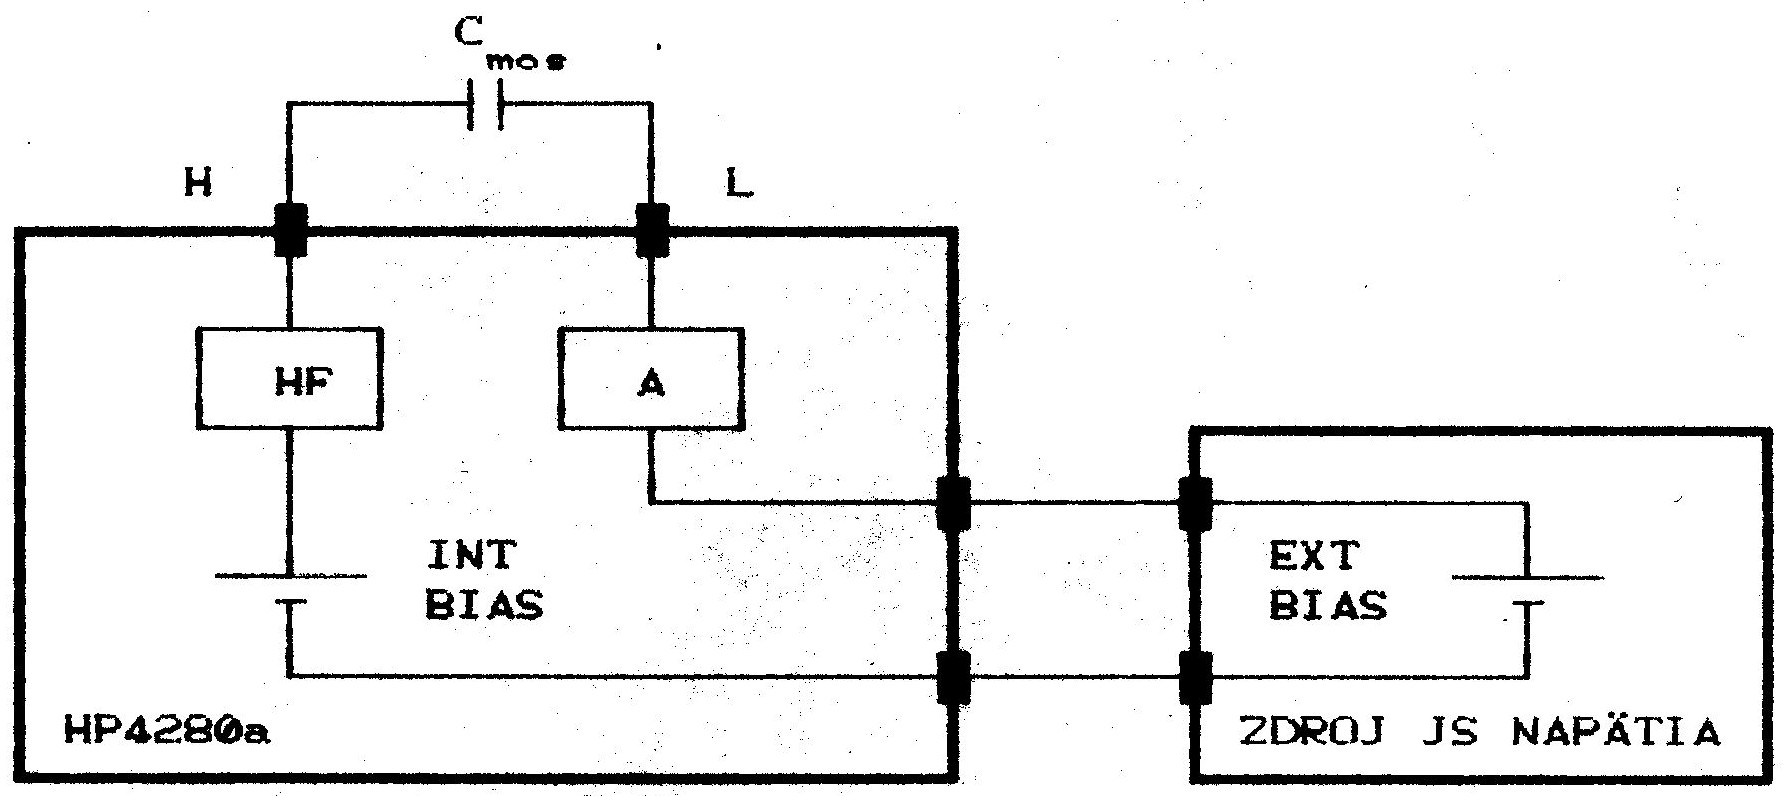
\includegraphics{Figures/fig-5-2.eps}
  \caption[Zapojenie prístrojov pre metódu konštantnej šírky
    OPN]{Zapojenie prístrojov pre metódu konštantnej šírky
    OPN.}\label{fig:5.2}
\end{figure}

Meranie závislosti $V_{g}(t)$ potom prebieha v nasledovných
krokoch. Pomocou externého zdroja JS napätia privedieme štruktúru MOS
do nerovnovážneho stavu. Zo zmeny kapacity $\Delta{C}$, ktorú
odmeriame prístrojom HP4280a, vypočítame pomocou vzťahu~\ref{eq:3.9}
požadovanú zmenu napätia hradla $\Delta{V_{g}}$. Ak je jej veľkosť v
absolútnej hodnote väčšia ako $0.001 V$ zmeníme hodnotu napätia hradla
o $\Delta{V_{g}}$, čím udržiavame konštantnú hodnotu nerovnovážnej
kapacity štruktúry MOS\@. Pri každej zmene napätia hradla odčítame
čas, kedy táto zmena nastala. Meranie závislosti $V_{g}(t)$ ukončíme,
ak uplynul čas merania (označme ho $T_{hold}$), ktorý zadáva operátor,
prípadne ak zmena hradlového napätia presiahla hraničné hodnoty
intervalu $(-2.0,+2.0) V$.  Experimentálne sa ukázalo, že programová
spätnoväzobná slučka zabezpečujúca konštantnú hodnotu kapacity pracuje
dostatočne rýchlo a presne. Počas prevádzaných experimentov bolo
kolísanie udržiavanej kapacity lepšie ako 1\%.

Meranie opakujeme pre rôzne hodnoty kapacity štruktúry MOS v
nerovnovážnom stave, aby sme mohli určiť generačnú dobu minoritných
nosičov náboja podľa vzťahu~\ref{eq:3.10}.

Parametrami riadiaceho programu je interval, v ktorom sa má pohybovať
hranica OPN $(W_{start}, W_{stop})$ s krokom $W_{step}$. Ďalším
parametrom je hodnota $T_{hold}$, ktorá udáva maximálnu dobu merania
jednej závislosti $V_{g}(t)$.

Riadiaci program vyžaduje pre svoju činnosť dátové súbory s nameranými
C-V závislosťami hlbokého ochudobnenia a kapacitami oxidovej vrstvy
testovaných štruktúr kremíkovej dosky. Pomocou týchto vopred
nameraných dát a zo zadanej vzdialenosti hranice OPN potom určuje
počiatočné hradlové napätie pre nastavenie externého zdroja JS
napätia.  Pre svoju činnosť potrebuje riadiaci program ešte jeden
dátový súbor, obsahujúci koncentračné profily dotujúcich prímesí
meraných štruktúr MOS\@. Hodnoty koncentrácie sú potrebné pri
vyčísľovaní zmeny napätia hradla štruktúry MOS podľa
vzťahu~\ref{eq:3.9}.

Po zmeraní závislosti $V_{g}(t)$ určíme lineárnou regresiou jej
smernicu. Z uskutočnených experimentov sa ukazuje, že minimálna doba
merania závislosti $V_{g}(t)$, kedy ešte možno očakávať akceptovateľné
výsledky je pre substráty s hodnotami $\tau_g$ rádove $10^{3}\mu{s}$
približne $T_{hold}=10s$. Počas tejto doby prichádzalo k zmene napätia
hradla v rozsahu $50-500 mV$ v závislosti od šírky OPN a v závislosti
od prírastku minoritných nosičov z oblasti mimo OPN\@. Zároveň bolo z
grafického znázornenia závislosti $\frac{dV_g}{dt}=f(w)$ vidieť vplyv
prírastku minoritných nosičov náboja z oblasti mimo OPN, čo sa
prejavilo približne rovnakým sklonom závislostí
$\frac{dV_g}{dt}=f(w)$, ale rôznou absolútnou hodnotou. Zo zobrazenia
závislostí $\frac{dV_g}{dt}=f(w)$ na celej kremíkovej doske vyplýva,
že akceptovateľné hodnoty $\tau_{g}$ možno počítať jedine z derivácie
funkcie $\frac{dV_g}{dt}=f(w)$ podľa w (vzťah~\ref{eq:3.10}
príp.~\ref{eq:3.7}) a v žiadnom prípade nie z jej funkčných hodnôt
(vzťah~\ref{eq:3.5}). Do výstupného dátového súboru sme ukladali
funkčné závislosti $\frac{dV_g}{dt}=f(w)$.

Z princípu metódy vyplýva minimálna vzdialenosť od povrchu polovodiča,
v ktorej je možno určovať $\tau_{g}$. Touto hranicou je šírka OPN
zodpovedajúca počiatku slabej inverzie v polovodiči.

\section{Časové diagramy použitých metód.}\label{sec:5.4}

Aby sme mohli odhadnúť dobu merania pre jednotlivé metódy, znázorníme
graficky časové závislosti hradlového napätia štruktúry MOS\@. Okrem
rovnovážnej HF C-V metódy, kde je celý priebeh merania riadený
procesorom prístroja HP4280a a jeho časový diagram je prevzatý z
manuálu~\cite{5.7}, boli časové diagramy určené na základe
experimentálne nameraných hodnôt. Tieto časové hodnoty sú závislé od
druhu riadiaceho počítača a od optimalizácie riadiacich programov. V
našom experimente sme použili osobný počítač PC AT, pracujúci na
frekvencii 10 MHz s koprocesorom 80287 (6 MHz) a pevným diskom s dobou
prístupu 28 ms. Riadiace programy boli kompilované bez optimalizácie
na rýchlosť s použitím emulačnej knižnice podprogramov pre matematické
operácie s plávajúcou čiarkou.

V spojení s časovými diagramami uvedieme aj rozsahy napätí použitých
prístrojov.

\par\emph{POZNÁMKA.} V prípade, ak je pri maximálnej hodnote časového
údaju uvedený údaj `neohraničené', znamená to, že jeho maximálna
veľkosť závisí od dátového typu zodpovedajúcej premennej riadiaceho
programu, prípadne od rozsahu prístroja.


\newpage
\subsection{Rovnovážna HF C-V závislosť.}\label{sec:5.4.1}

\begin{figure}[h!]\centering
  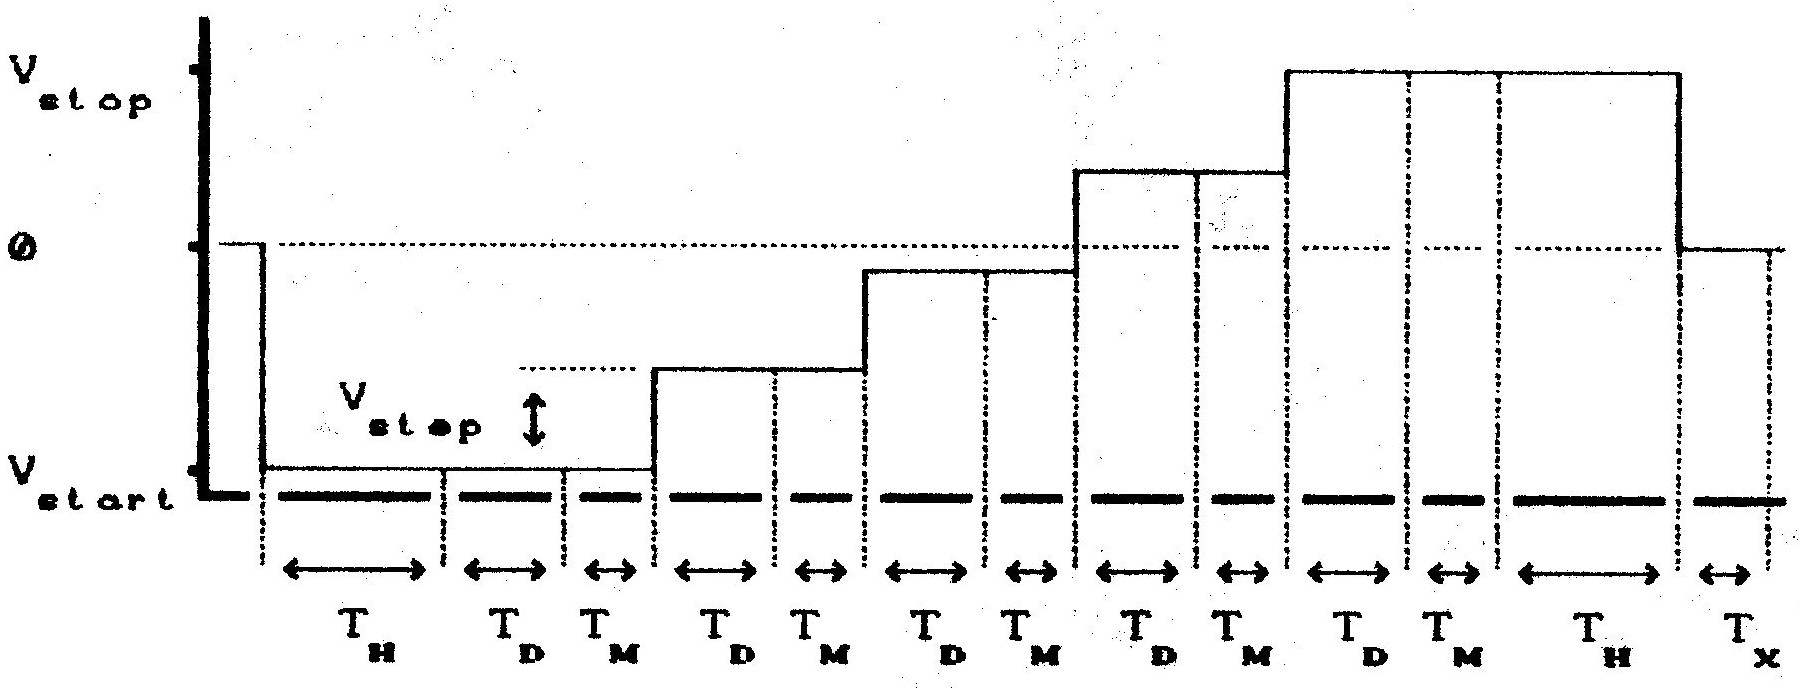
\includegraphics{Figures/fig-5-3.eps}
  \caption[Časový diagram rovnovážnej HF C-V metódy]{Časový diagram
    rovnovážnej HF C-V metódy.}\label{fig:5.3}
\end{figure}

\begin{table}[h!]\centering
  \begin{tabular}{l p{0.5\linewidth} l l}
    param.      & popis parametra & min. & max.hodnota\\
    \hline% chktex-file 44
    $T_H$       & čas ustálenia \dotfill & $3 ms$ &  $650 s$\\
    $T_D$       & čas pozdržania merania \dotfill & $3 ms$ & $650 s$\\
    $T_M$       & čas merania \dotfill & $40 ms$\\
    $T_X$       & binárny prenos dát,\\
                & predspracovanie dát,\\
                & uloženie dát do súboru,\\
                & posuv stolíka na ďalšiu štruktúru \dotfill & $\sim 7 s$\\
    $V_{start}$ & \dotfill & $-100.0 V$ & $+100.0 V$\\
    $V_{stop}$  & \dotfill & $-100.0 V$ & $+100.0 V$\\
    $V_{step}$  & \dotfill & $\pm 0.001 V$ & $\pm 200.0 V$\\
    \hline
  \end{tabular}
  \caption[Časový diagram rovnovážnej HF C-V metódy]{Časový diagram
    rovnovážnej HF C-V metódy.}\label{tab:5.1}
\end{table}

\newpage
\subsection{Nerovnovážna HF C-V závislosť.}\label{sec:5.4.2}

\begin{figure}[h!]\centering
  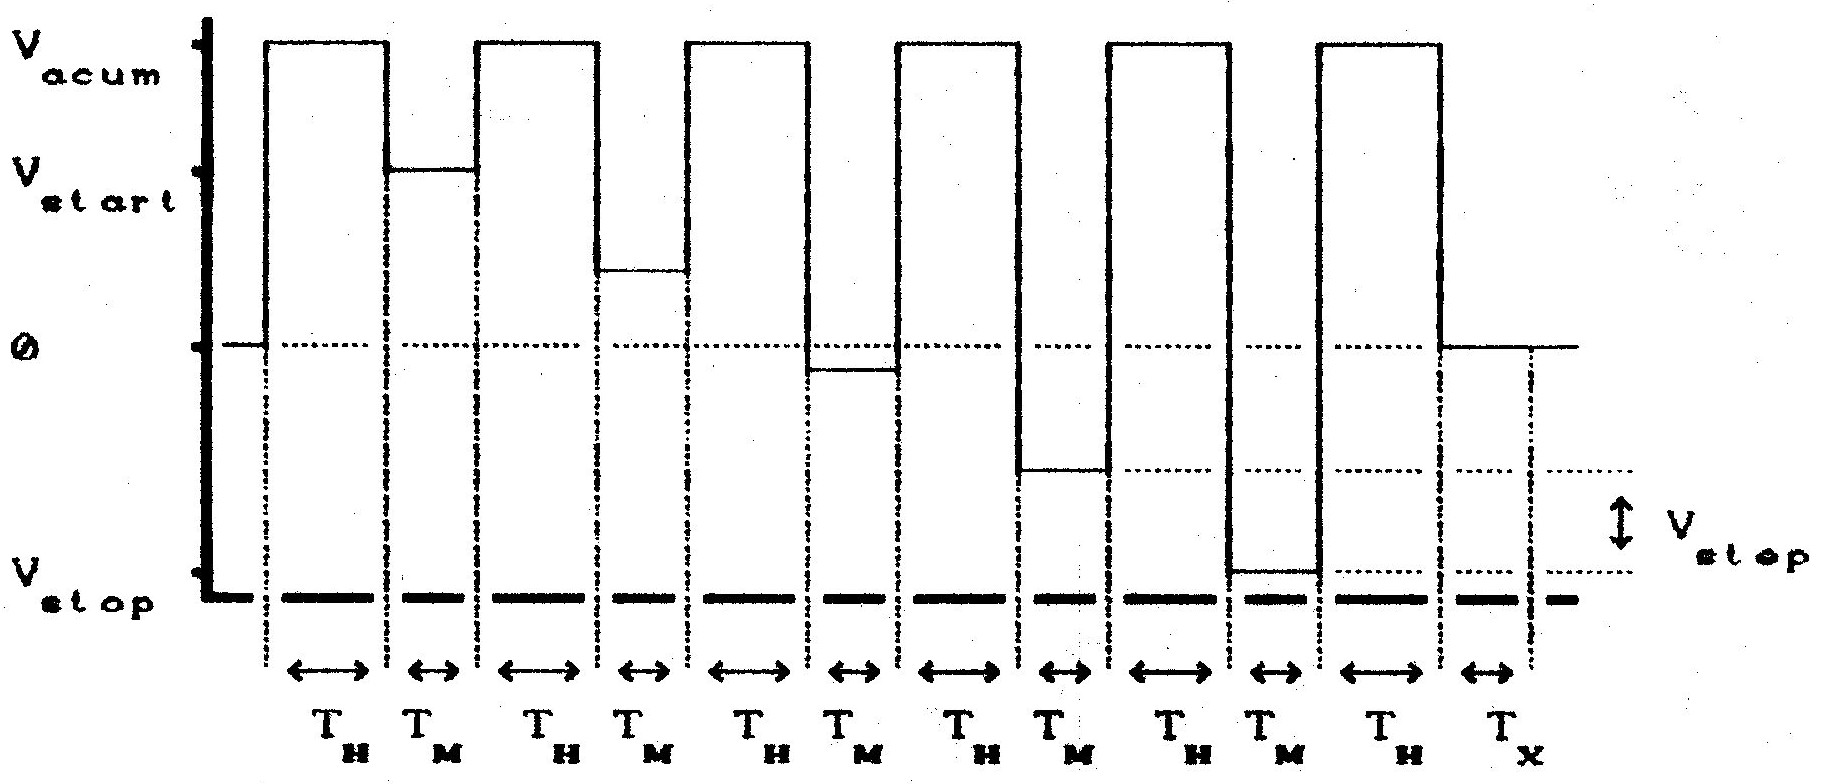
\includegraphics{Figures/fig-5-4.eps}
  \caption[Časový diagram nerovnovážnej HF C-V metódy]{Časový diagram
    nerovnovážnej HF C-V metódy.}\label{fig:5.4}
\end{figure}

\begin{table}[h!]\centering
  \begin{tabular}{l p{0.5\linewidth} l l}
    param.      & popis parametra & min. & max.hodnota\\
    \hline
    $T_H$       & čas relaxácie minoritných nosičov náboja \dotfill & $0 s$ &  neohraničené\\
    $T_M$       & čas merania a prenos dát \dotfill & $330 ms$\\
    $T_X$       & predspracovanie dát,\\
                & uloženie dát do súboru,\\
                & posuv stolíka na ďalšiu štruktúru \dotfill & $\sim 4s$\\
    $V_{start}$ & \dotfill & $-100.0$ & $+100.0 V$\\
    $V_{stop}$  & \dotfill & $-100.0$ & $+100.0 V$\\
    $V_{step}$  & \dotfill & $\pm 0.001$ & $\pm 200.0 V$\\
    $V_{acum}$  & \dotfill & $-100.0$ & $+100.0 V$\\
    \hline
  \end{tabular}
  \caption[Časový diagram nerovnovážnej HF C-V metódy]{Časový diagram
    nerovnovážnej HF C-V metódy.}\label{tab:5.2}
\end{table}

\newpage
\subsection{Kvázistatická C-V závislosť.}\label{sec:5.4.3}

\begin{figure}[h!]\centering
  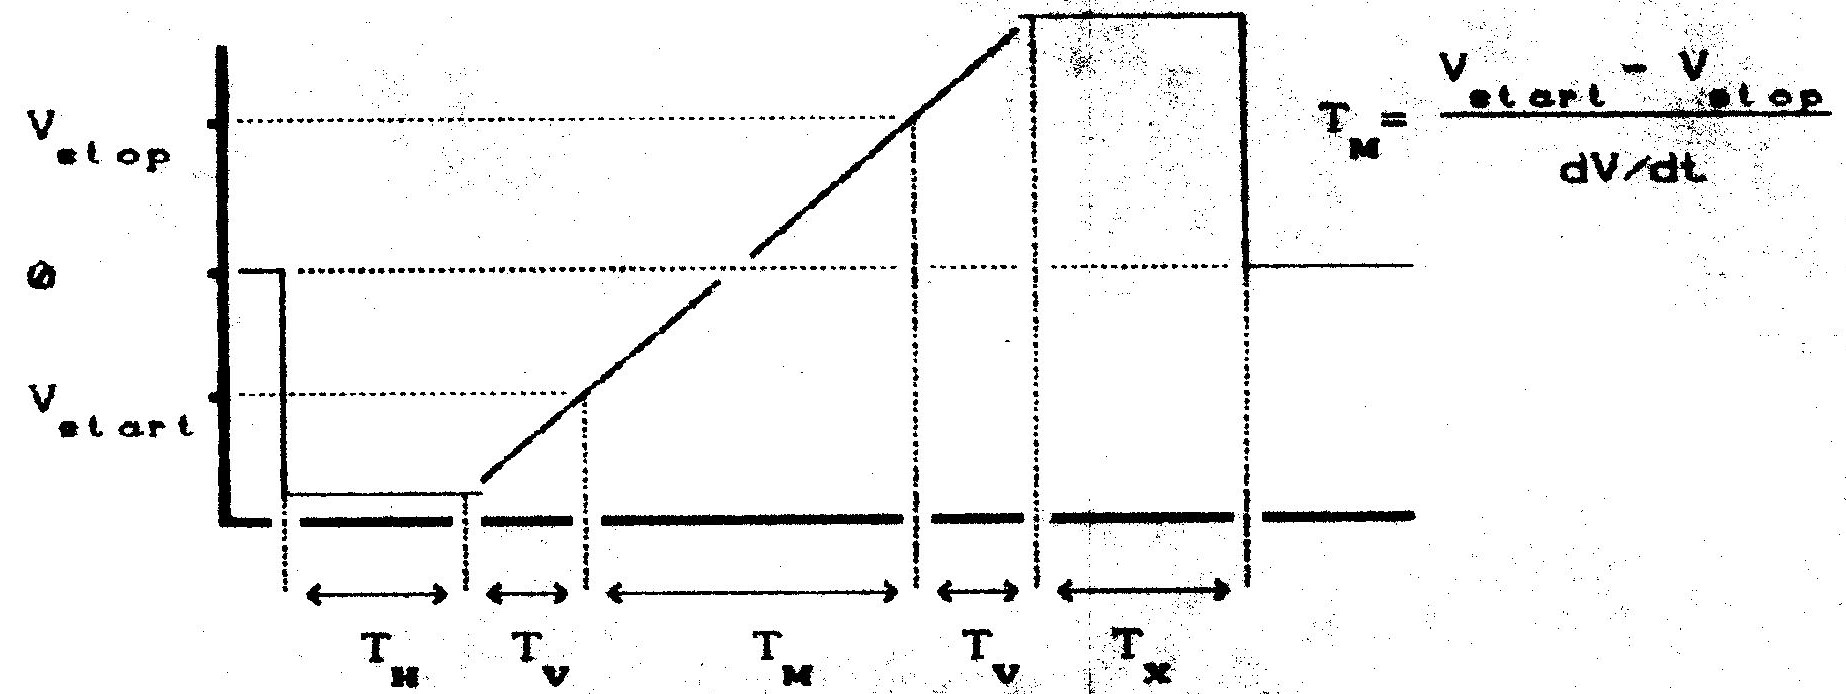
\includegraphics{Figures/fig-5-5.eps}
  \caption[Časový diagram kvázistatickej C-V metódy]{Časový diagram
    kvázistatickej C-V metódy.}\label{fig:5.5}
\end{figure}

\begin{table}[h!]\centering
  \begin{tabular}{ l p{0.5\linewidth} l l }
    parameter   & popis parametra & min. & max.hodnota\\
    \hline
    $T_H$       & čas ustálenia \dotfill & $0 s$ & neohraničené\\
    $T_V$       & merania napätia hradla a času \dotfill & $5 s$\\
    $T_M$       & merania prúdu a času \dotfill & neohraničené\\
    $T_X$       & predspracovanie dát,\\
                & uloženie dát do súboru,\\
                & posuv stolíka na ďalšiu štruktúru \dotfill & $\sim 15s$\\
    $V_{start}$ & \dotfill & $-20.0$ & $+20.0 V$\\
    $V_{stop}$  & \dotfill & $-20.0$ & $+20.0 V$\\
    $dV/dt$     & \dotfill & $\pm 0.1mV/s$ & $\pm 10.0V/s$\\
    \hline
  \end{tabular}
  \caption[Časový diagram kvázistatickej C-V metódy]{Časový diagram
    kvázistatickej C-V metódy.}\label{tab:5.3}
\end{table}

\newpage
\subsection{Metóda konštantnej šírky OPN.}\label{sec:5.4.4}

\begin{figure}[h!]\centering
  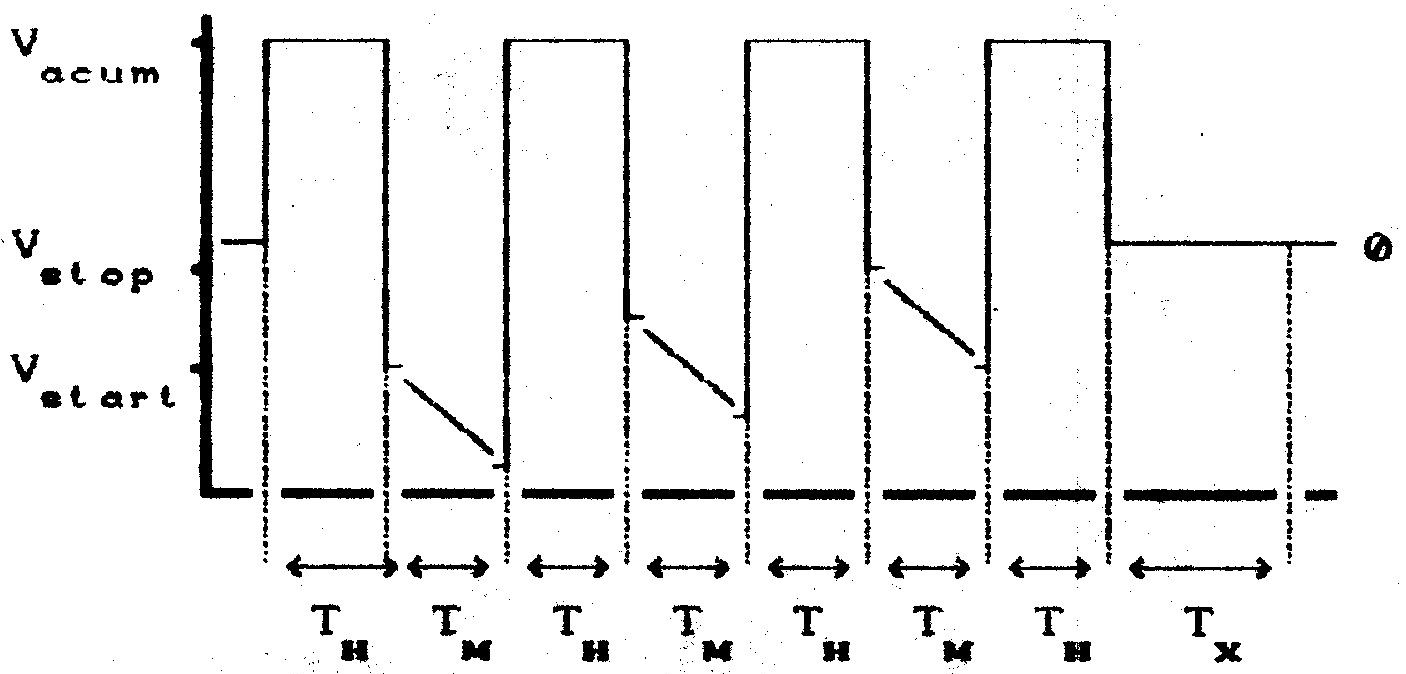
\includegraphics{Figures/fig-5-6.eps}
  \caption[Časový diagram metódy konštantnej šírky OPN]{Časový diagram
    metódy konštantnej šírky OPN}.\label{fig:5.6}
\end{figure}

\begin{table}[h!]\centering
  \begin{tabular}{ l p{0.5\linewidth} l l }
    param.      & popis parametra & min. & max.hodnota\\
    \hline
    $T_H$       & čas relaxácie minoritných nosičov náboja \dotfill & $0 s$ & neohraničené\\
    $T_M$       & čas merania, výpočet $dV/dt$ \dotfill & $10 s$ & neohraničené\\
    $T_X$       & uloženie dát do súboru,\\
                & posuv stolíka na ďalšiu štruktúru \dotfill & $\sim 2s$\\
    $V_{start}$ & \dotfill & $-40.0$ & $+40.0 V$\\
    $V_{stop}$  & \dotfill & $-40.0$ & $+40.0 V$\\
    $V_{acum}$  & \dotfill & $-40.0$ & $+40.0 V$\\
    \hline
  \end{tabular}
  \caption[Časový diagram metódy konštantnej šírky OPN]{Časový diagram
    metódy konštantnej šírky OPN.}\label{tab:5.4}
\end{table}


\begin{thebibliography}{}
\bibitem[5.1]{5.1} Mariassy P.: Riadiaca jednotka prístroja typu
  talker/listener na spojenie so zbernicou IMS\@. Diplomová práca. EF
  SVŠT Bratislava 1988.
\bibitem[5.2]{5.2} National Instruments, IEEE-488 Instrumentation
  Interface. User guide.
\bibitem[5.3]{5.3} Keithley model 642, Instruction manual.
\bibitem[5.4]{5.4} Marčuk G.I.: Metódy numerické matematiky. Academia
  Praha 1987.
\bibitem[5.5]{5.5} Cox M.G.: J. Inst. Maths. Aplics., 10 (1972) s.134.
\bibitem[5.6]{5.6} De Boor C.: J. Approx. Theory, 6 (1972) s.50.
\bibitem[5.7]{5.7} Hewlett-Packard, Operational and service manual,
  Model HP4280a.
\end{thebibliography}
 
% Chapter 6

\chapter{Spracovanie dát a zobrazenie získanych parametrov štruktúr MOS.} % Main chapter title

\label{Chapter6} % For referencing the chapter elsewhere, use \ref{Chapter1} 

\lhead{Chapter 6. \emph{Spracovanie dát a zobrazenie získaných parametrov štruktúr MOS}}

V tejto kapitole uvedieme stručne postup spracovania dát, nameraných
pomocou programov zberu dát a zameriame sa na plošné zobrazenie
získaných parametrov štruktúr MOS. Metodika výpočtu parametrov
štruktúr MOS bola popísaná v kapitolách 3 a 4, na ktoré sa budeme
odvolávať.

Väčšina parametrov je určovaná z nameraných dát pomocou samostatných
programov a ukladaná do dátových súborov, ktorých štruktúra bola
popísaná v časti 5. Plošné rozloženie vypočítaných parametrov štruktúr
MOS možno potom zobraziť na displeji počítača. Pri zobrazovaní na
displeji je k dispozícii 16 farieb, avšak pri zobrazení obrázkov na
tlačiarni bolo kvôli lepšej rozlišiteľnosti použitých len 6
farieb. Orientácia kremíkovej dosky na obrázkoch je smerom 'fazetou
hore', pričom jeden štvorček zobrazenej plochy predstavuje hodnotu
parametra štruktúry MOS. Farba štvorčeka závisí od intervalu, do
ktorého daná hodnota spadá. Škála intervalov je zobrazená v pravej
časti obrázku, pričom číslo uvedené pri jednotlivých farbách
predstavuje dolnú hranicu intervalu. Pretože sa farby v škále
intervalov viackrát opakujú, bolo potrebné označiť, v ktorých
intervaloch sa zobrazované hodnoty nachádzajú. To je označené veľkým
písmenom 'X' medzi dolnou hranicou intervalu a prislúchajúcou
farbou. Možno ešte poznamenať, že náhodne odlišné výsledky v
niektorých bodoch kremíkovej dosky spôsobia, že sa v škále intervalov
objaví vyznačený interval, ktorý zjavne nesúvisí s ostatnými
hodnotami, čo možno pripísat nefunkčnej štruktúre MOS. Treba ešte
upozorniť, že orientácia škály sa môže pri zobrazení rôznych
parametrov meniť.

\section{Určenie koncentračného profilu dotujúcich prímesí, dávky implantácie a napätia vyrovnaných pásov.}\label{sec:6.1}

Určenie koncentračného profilu dotujúcich prímesí vykonáva samostatný
program, ktorý ako vstupné dáta vyžaduje súbory (a) nameraných HF C-V
závislostí a (b) nameraných kapacít oxidovej vrstvy štruktúry
MOS. Výstupom programu je dátový súbor obsahujúci hĺbkové priebehy
koncentračných profilov skúmaných štruktúr MOS, ktoré sú počítané
podľa vzťahov uvedených v časti \ref{sec:4.1}. Ak boli v procese zberu
dát zmerané aj kvázistatické C-V závislosti, program vykoná korekciu
koncentračného profilu na hustotu pascí rozhrania
$Si-SiO_2$. Povrchový potenciál určujeme podľa vzťahov \ref{eq:4.3} a
\ref{eq:4.4} a používame ho pre korekciu aproximácie hlbokého
ochudobnenia pri povrchu polovodiča a pre výpočet hĺbky (šírky
OPN). Vedľajším produktom je dátovy súbor obsahujúci napätia
vyrovnaných pásov $V_{fb}$, ktoré sa určujú v bode C-V závislosti, pre
ktoré povrchový potenciál $\varphi_s$ mení znamienko. Obrázok
\ref{fig:6.1} predstavuje plošné rozloženie koncentrácie v rôznych
hĺbkach polovodiča a na obrázku \ref{fig:6.2} je znázornené rozloženie
$V_{fb}$. Koncentračný profil prímesí bol vytvorený implantáciou
$P^{31}$ s dávkou $4.0\times 10^{15} m^{-2}$ pri energii $120
keV$. Aktivácia prebiehala počas 40 minút pri teplote $1050 \degree C$
v atmosfére $N_2$. Stredná hodnota $N(x)$ je spolu s ďalšími priebehmi
pre rôzne implantačné dávky zobrazená na obrázku \ref{fig:7.3}.

Pre známe priebehy koncentračných profilov môžeme vypočítať dávku
implantácie podľa vzťahu

\begin{equation}\label{eq:6.1}
D = \int_{0}^{x_{1}}(N(x) - N_{b}) dx
\end{equation}

kde predpokládame, že poznáme priebeh N(x) do vzdialenosti $x_{1}$ ,
pre ktorú platí

\begin{equation}\label{eq:6.2}
N(x) = N_{b} \qquad {x \ge x_{1}}
\end{equation}

Dávka $D$ vypočítaná týmto spôsobom predstavuje časť implantovaných
iónov, ktoré sa dostali v priebehu implantácie do polovodiča a boli
aktivované v poimplantačnom tepelnom spracovaní. Na obrázku
\ref{fig:6.3} je znázornené plošné rozloženie dávky na testovanej
kremíkovej doske určenej zo závislosti $N(x)$ zobrazených na obrázku
\ref{fig:6.1}.

\begin{figure}[h!]\centering
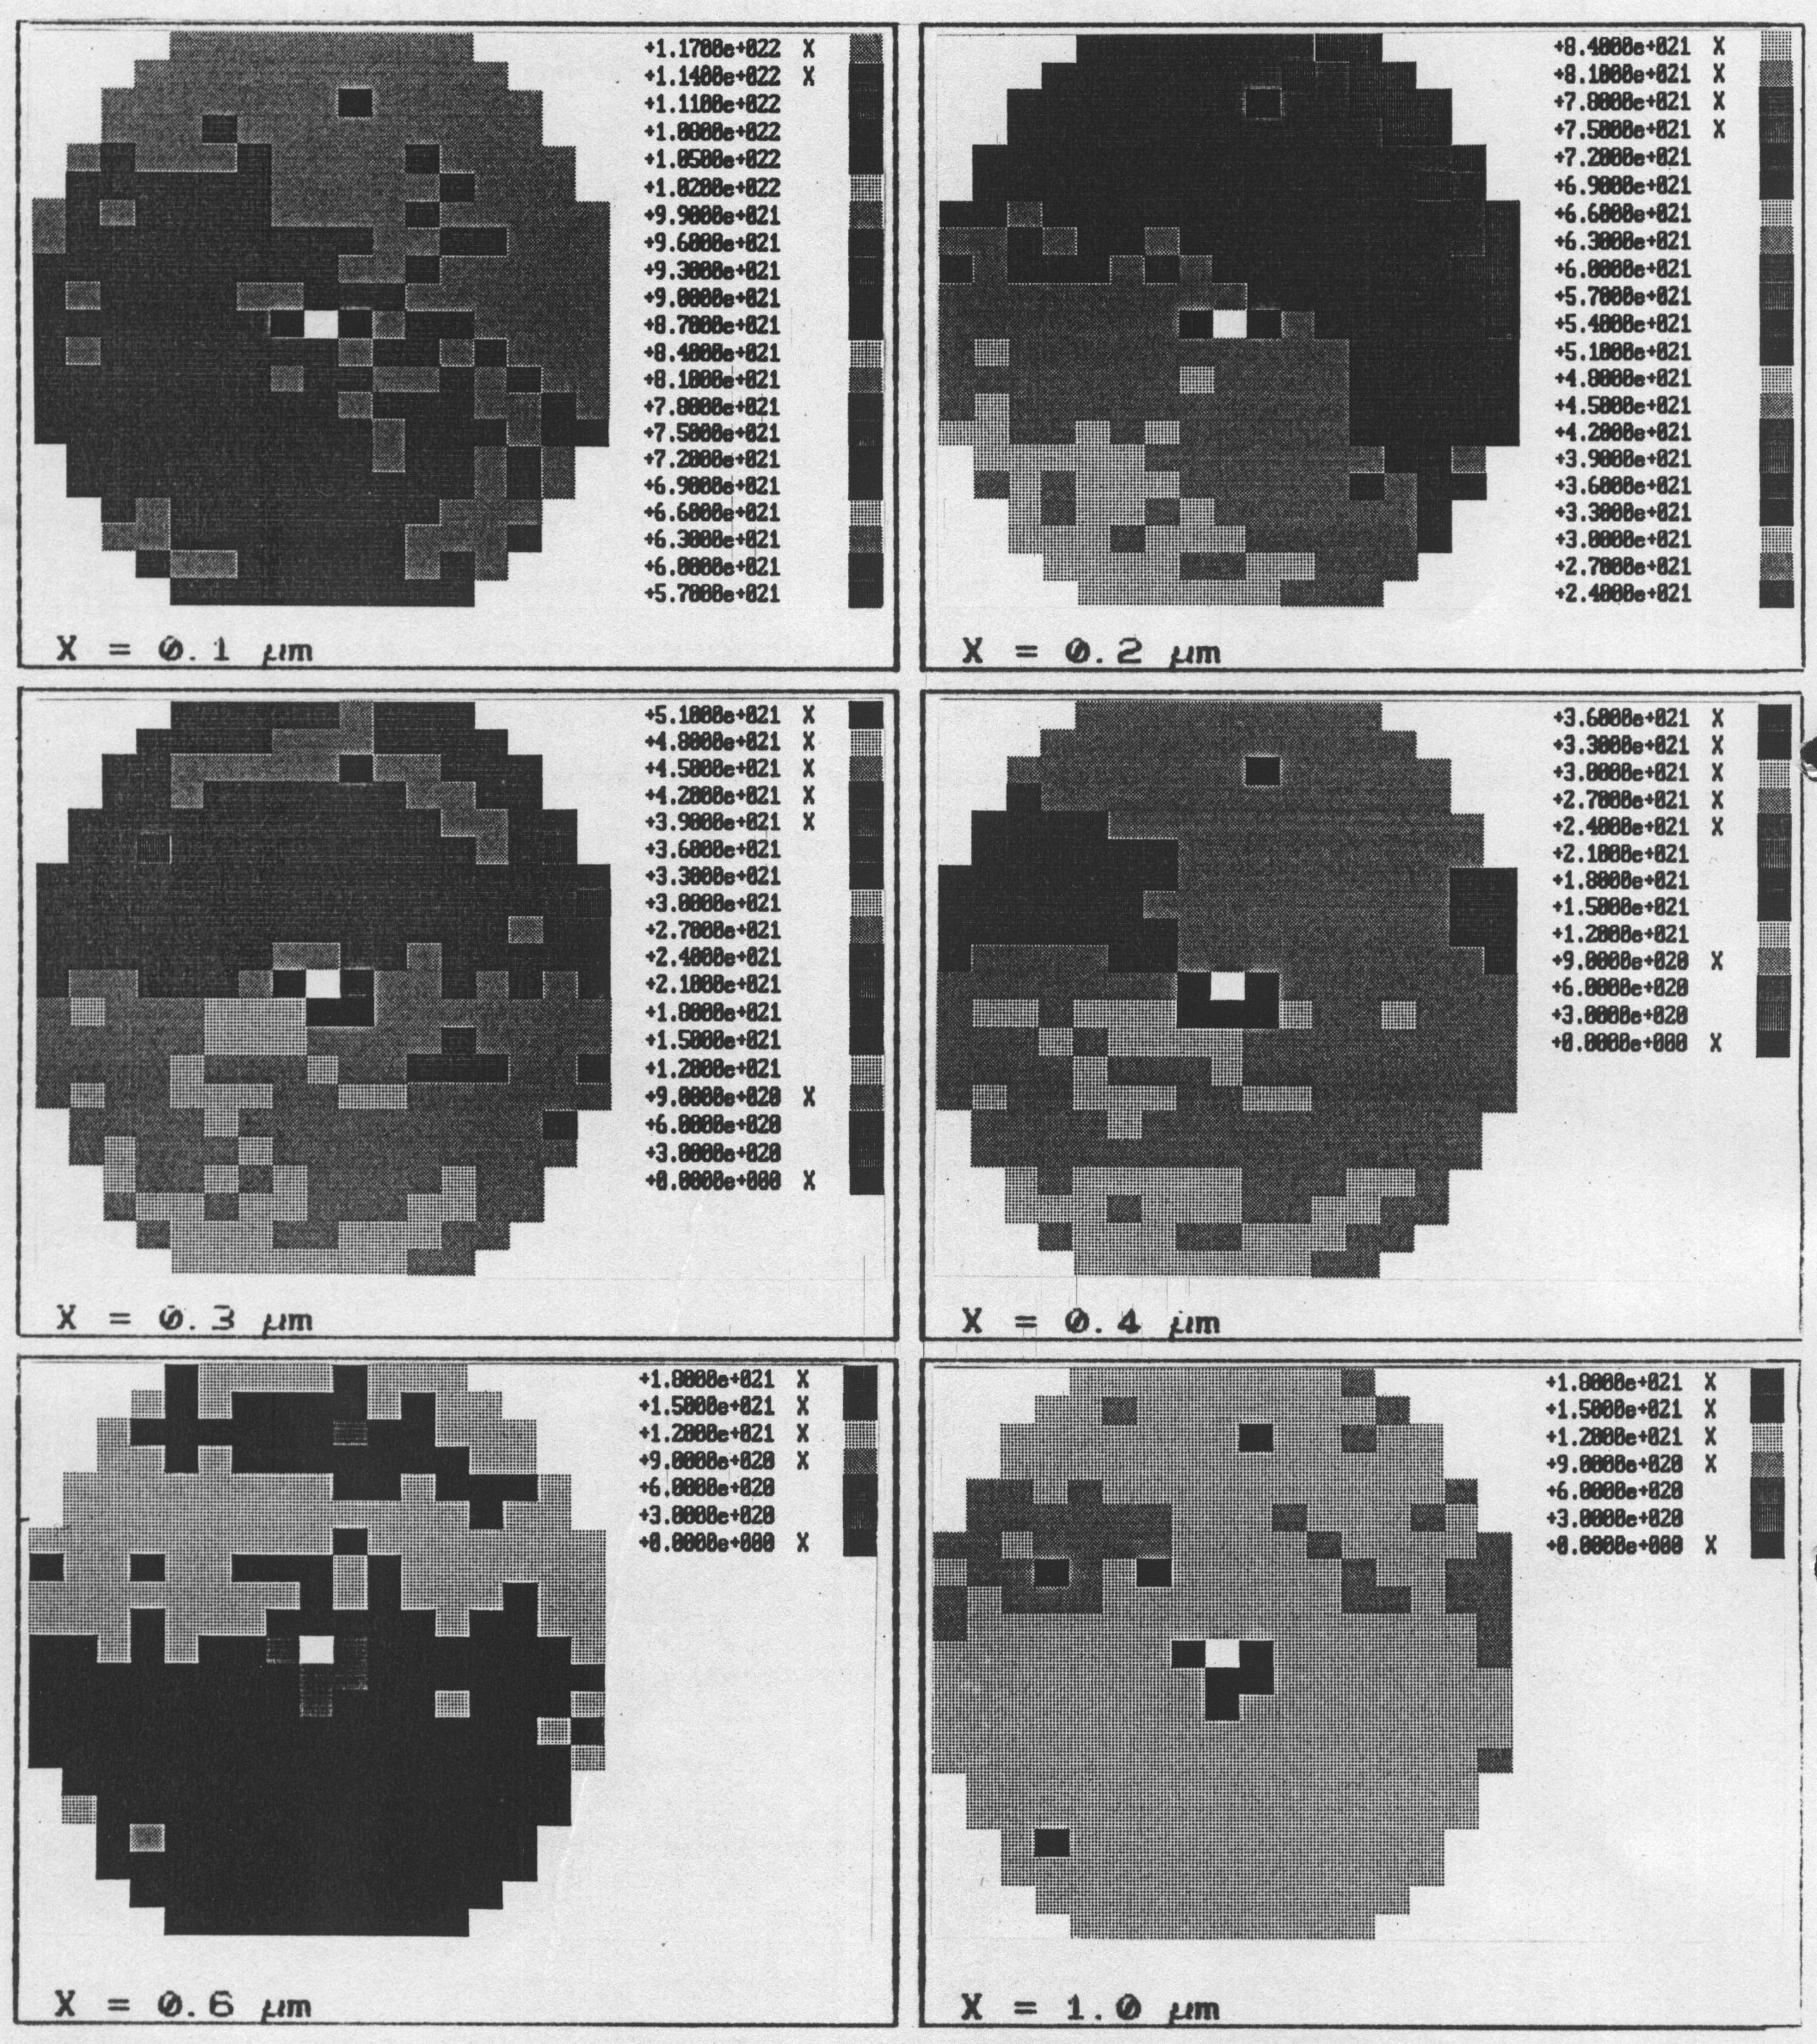
\includegraphics{Figures/fig-6-1.eps}
\captionsetup{justification=raggedright, singlelinecheck=false}
\caption[Rozloženie dotujúcich prímesí $N(x)$ v rôznej hĺbke
  $x$]{Rozloženie dotujúcich prímesí $N(x)$ v rôznej hĺbke $x$ pod
  povrchom polovodiča pre dávku implantácie $4.0 \times 10^{15}
  m^{-2}$.}
\label{fig:6.1}
\end{figure}

\begin{figure}[h!]\centering
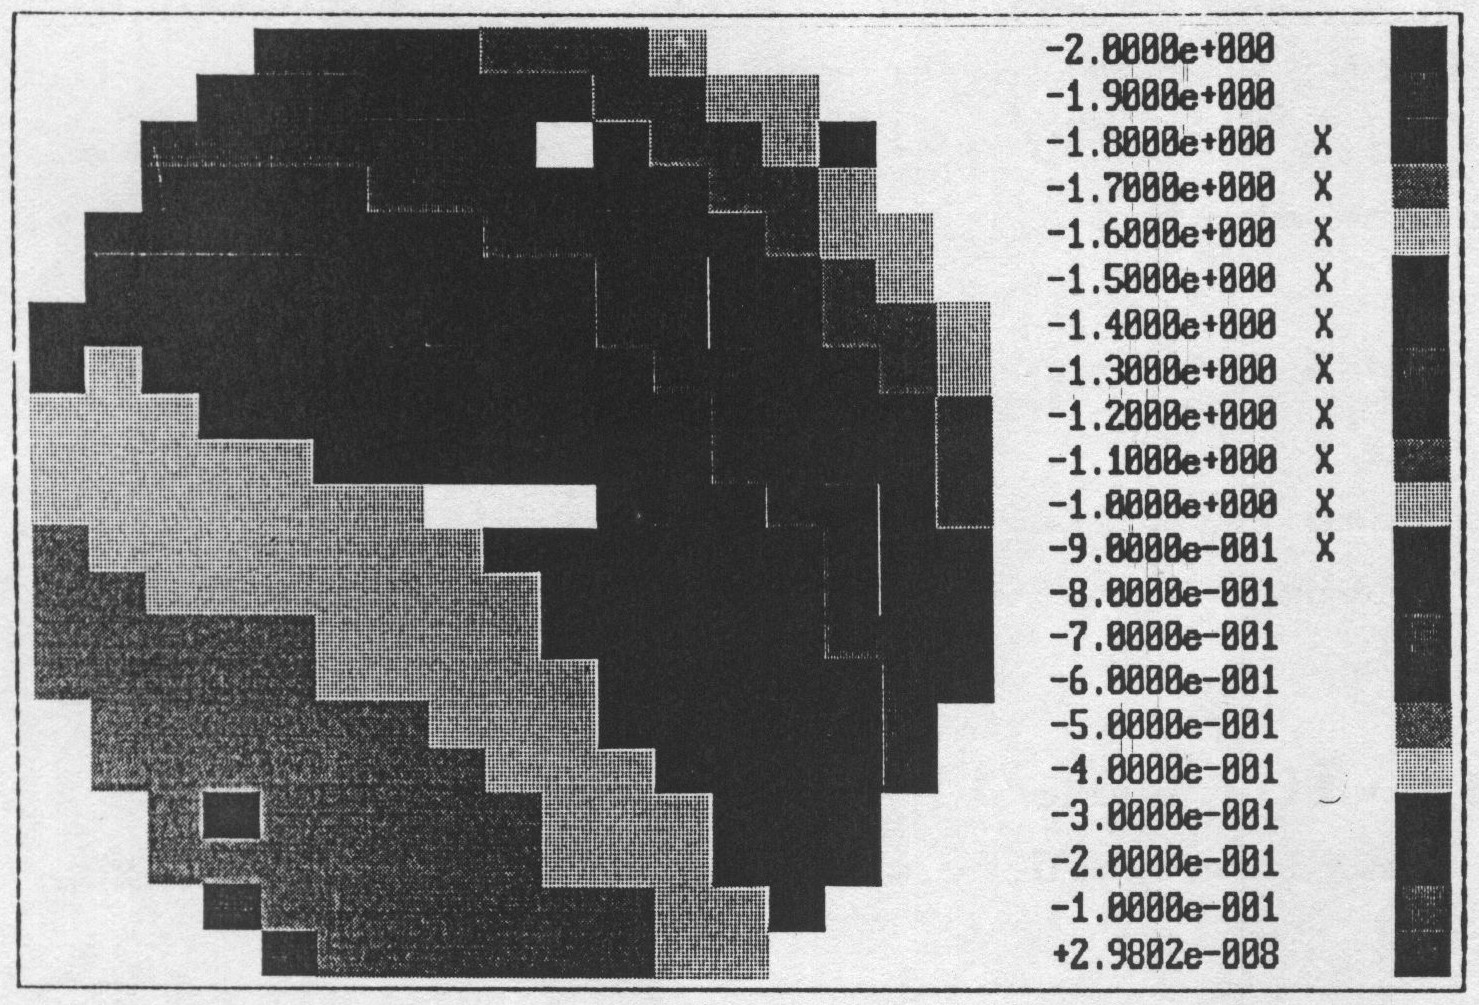
\includegraphics{Figures/fig-6-2.eps}
\captionsetup{justification=raggedright, singlelinecheck=false}
\caption[Plošné rozloženie $V_{fb}$]{Plošné rozloženie $V_{fb}$ určené
  pri výpočte $N(x)$ z obrázka \ref{fig:6.1}.}
\label{fig:6.2}
\end{figure}

\begin{figure}[h!]\centering
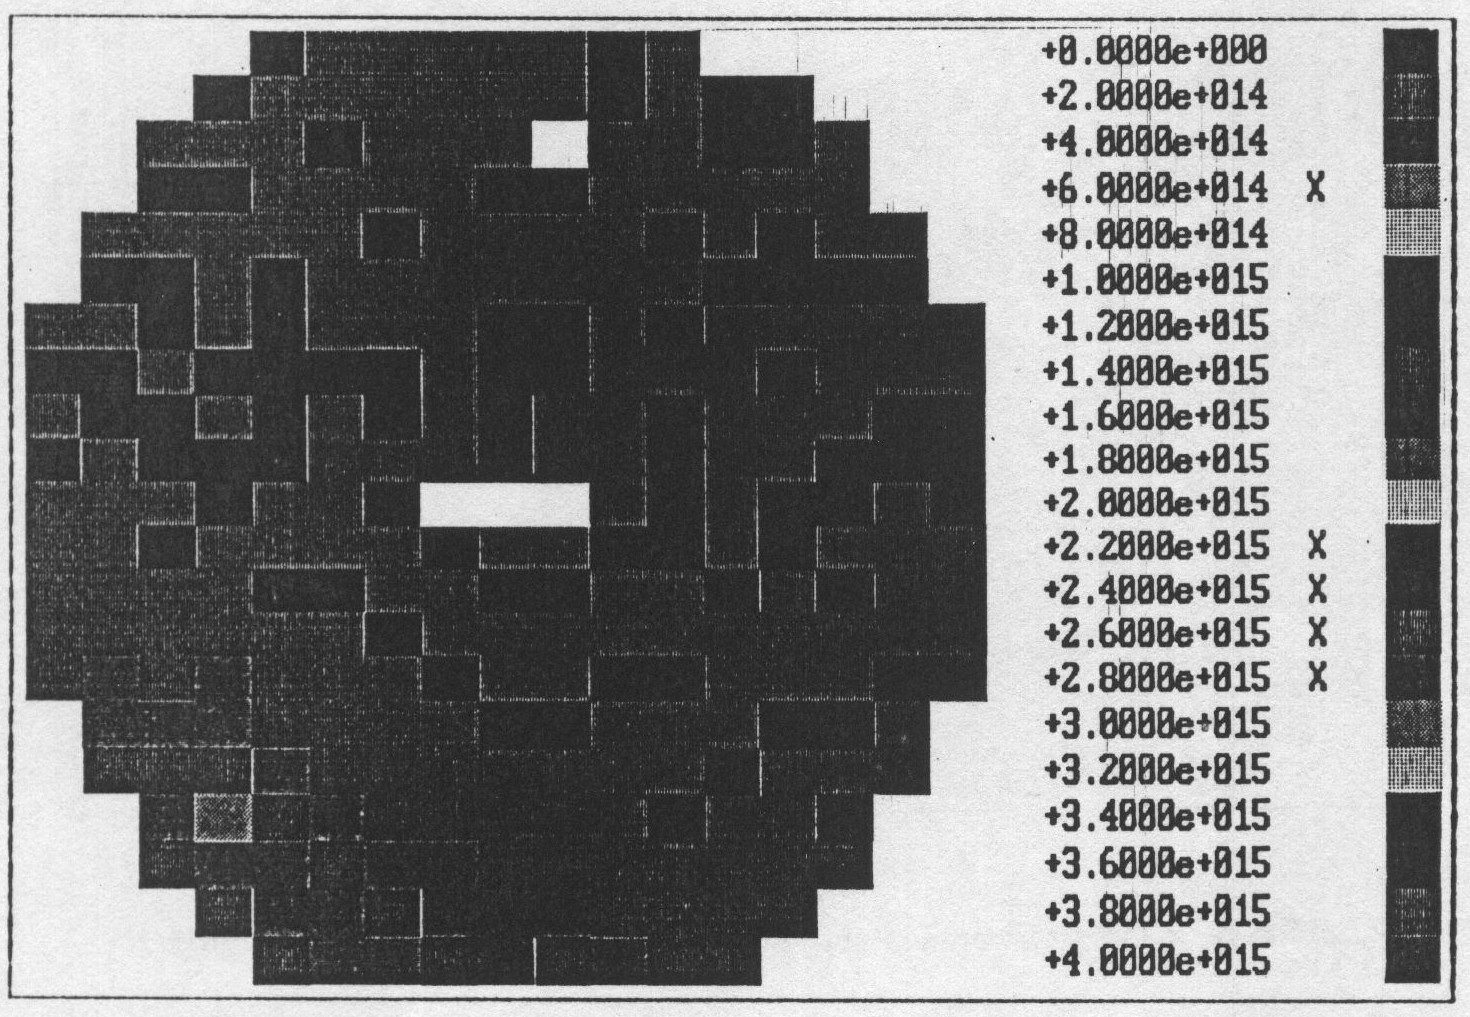
\includegraphics{Figures/fig-6-3.eps}
\captionsetup{justification=raggedright, singlelinecheck=false}
\caption[Plošné rozloženie nameranej dávky implantácie]{Plošné
  rozloženie nameranej dávky implantácie pre profil N(x) z obrázka
  \ref{fig:6.1}.}
\label{fig:6.3}
\end{figure}


\section{Určenie hrúbky oxidovej vrstvy.}\label{sec:6.2}

Ak poznáme kapacitu oxidovej vrstvy štruktúry MOS a jej plochu, potom
môžeme vypočítať jej hrúbku podľa vzťahu

\begin{equation}\label{eq:6.3}
h_{ox} = A \frac{\epsilon}{C_{ox}}
\end{equation}

kde sme použili hodnotu relatívnej permitivity $SiO_{2}$
$\epsilon_{r}=3.9$. Plošné rozloženie hrúbky oxidovej vrstvy je potom
zobrazené na obrázku \ref{fig:6.4}.

\begin{figure}[h!]\centering
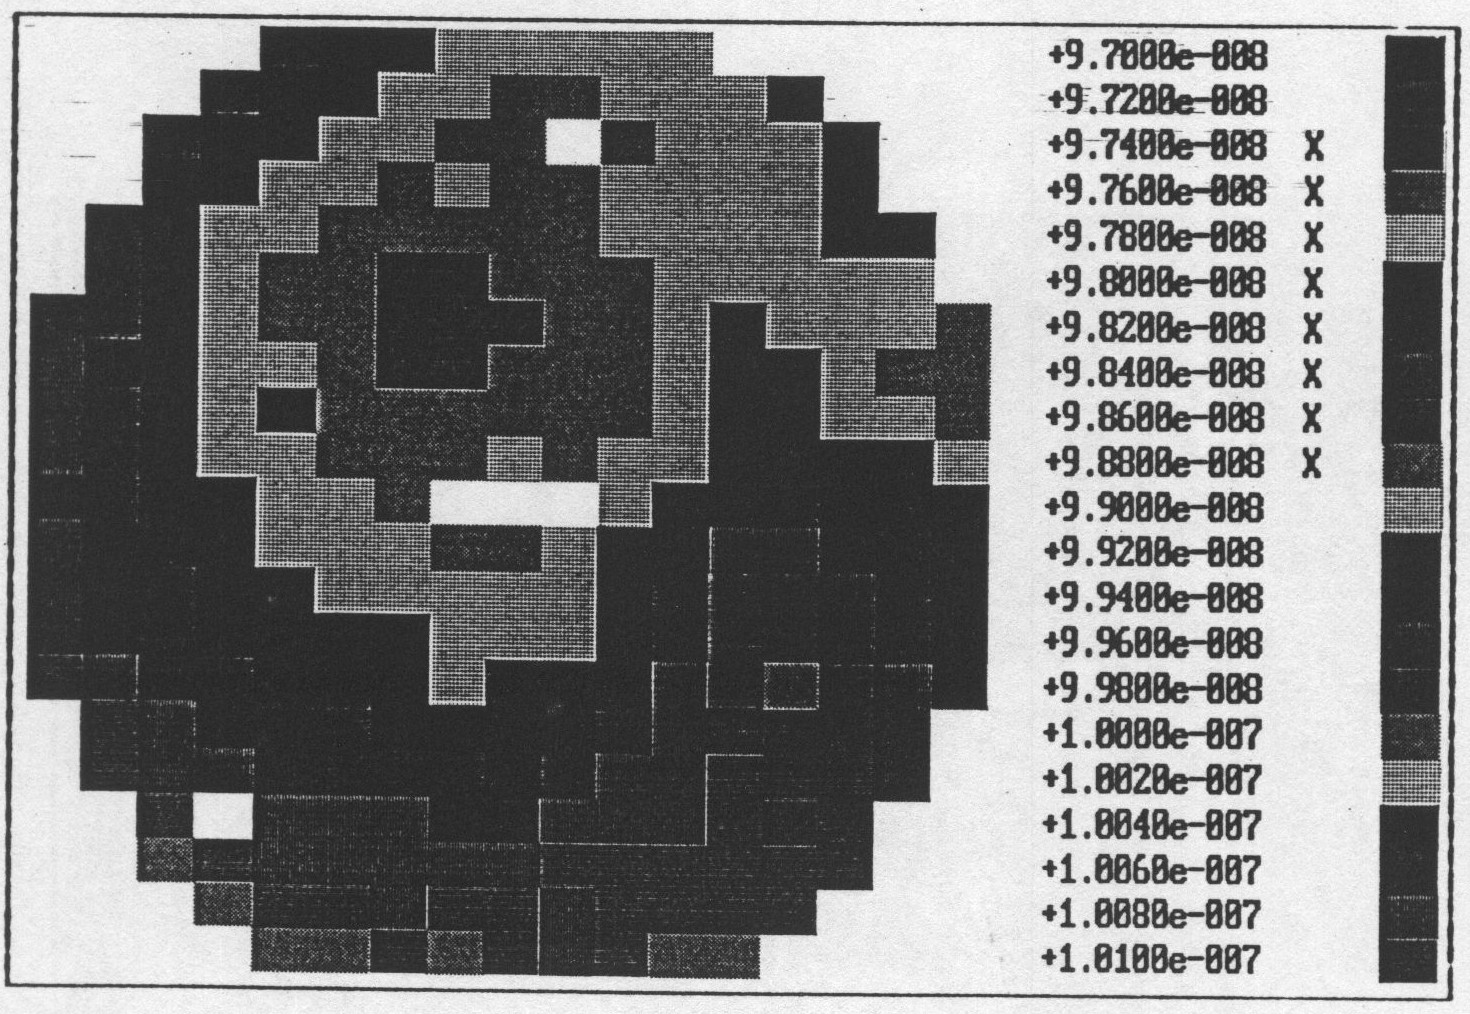
\includegraphics{Figures/fig-6-4.eps}
\captionsetup{justification=raggedright, singlelinecheck=false}
\caption[Plošné rozloženie hrúbky hradlového oxidu $h_{ox}$]{Plošné
  rozloženie hrúbky hradlového oxidu $h_{ox}$.}
\label{fig:6.4}
\end{figure}


\section{Určenie hustoty pascí rozhrania $Si-SiO_{2}$.}\label{sec:6.3}

Pre výpočet hustoty pascí rozhrania použijeme porovnanie HF a
kvázistatickej C-V závislosti, kde použijeme postup popísany v časti
\ref{sec:4.2.1}. Možno poznamenať, že pre určenie polohy Fermiho
hladiny na povrchu polovodiča použijeme hodnoty povrchového potenciálu
$\varphi_{s}(V_{g})$, získané integráciou kvázistatickej C-V
závislosti a hodnotu integračnej konštanty $\varphi_{s0}$ určíme
postupom popísaným v dodatku \ref{app:AppendixG}.

Celý postup výpočtu $D_{it}$ je realizovaný dvoma programami. Prvý program na základe zmeraných kvázistatických C-V závislostí a známych hĺbkových priebehov $N(x)$ vypočíta závislosti $\varphi_{s}(V_{g})$, ktoré uloží do dátového súboru.  Druhý program pre svoju činnosť vyžaduje dátove súbory

\begin{itemize}
\item HF C-V závislosti $C_{mos}^{HF}(V_{g})$
\item kvázistatické C-V závislosti $C_{mos}^{LF}(V_{g})$
\item závislosť povrchového potenciálu od napätia hradla $\varphi_{s}(V_{g})$.
\end{itemize}

Vypočítané hodnoty $D_{it}$ ako závislosť polohy Fermiho hladiny v
zakázanom pásme polovodiča uloží do dátoveho súboru. Na obrázku
\ref{fig:6.5} je zobrazené plošné rozloženie $D_{it}$ v strede
zakázaného pásma.

\begin{figure}[h!]\centering
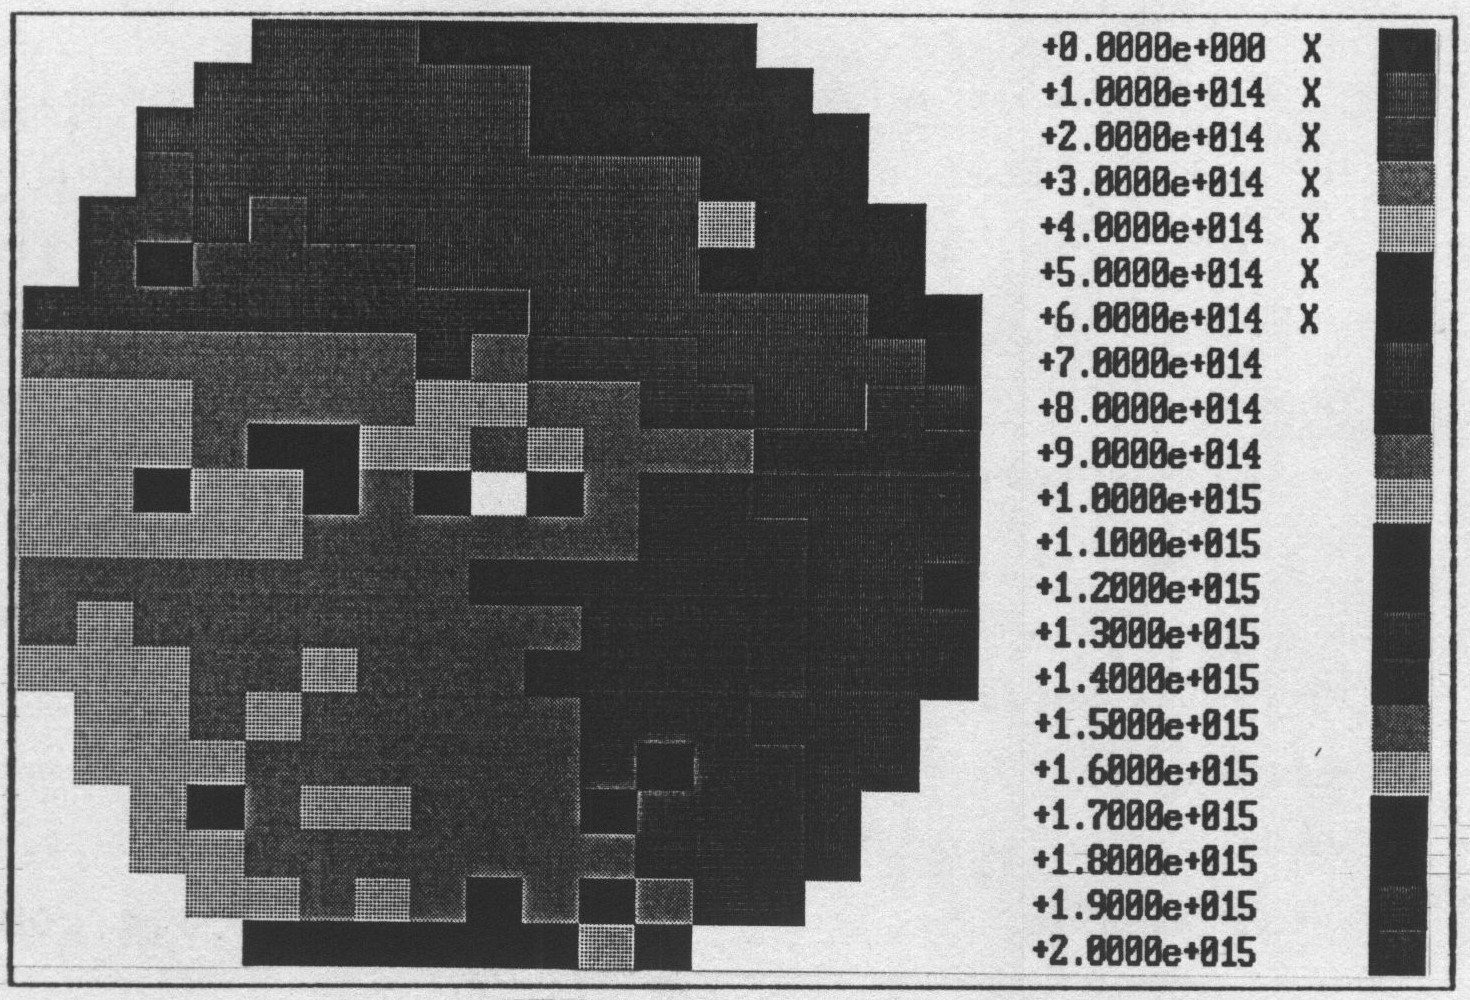
\includegraphics{Figures/fig-6-5.eps}
\captionsetup{justification=raggedright, singlelinecheck=false}
\caption[Plošné rozloženie hustoty pascí rozhrania $Si-SiO_{2}$ v
  strede zakázaného pásma]{Plošné rozloženie hustoty pascí rozhrania
  $Si-SiO_{2}$ v strede zakázaného pásma.}
\label{fig:6.5}
\end{figure}


\section{Určenie generačného času života minoritných nosičov náboja.}\label{sec:6.4}

V procese zberu dát metódou konštantnej šírky OPN bol vytvorený dátovy
súbor obsahujúci smernice závislostí $V_{g}(t)$ pre rôzne šírky OPN
testovaných štruktúr MOS kremíkovej dosky. Pre určenie generačného
času života minoritných nosičov náboja podľa vzťahu \ref{eq:3.10} je
dôležité ako vypočítame deriváciu závislosti smerníc $V_{g}(t)$ podľa
vzdialenosti hranice OPN od povrchu polovodiča. Použitie číslicových
filtrov v tomto prípade nie je vhodné, pretože máme k dispozícii málo
bodov závislosti $dV_{g}/dt = f(w)$. V tomto prípade možno pužiť
aproximáciu lokálnymi polynómami. Teoretický základ aj zdrojový text
procedúry v jazyku Algol je uvedený napríklad v \cite{6.1}. Na obrázku
\ref{fig:6.6} je zobrazené plošné rozloženie generačnej doby
minoritných nosičov náboja, ktorá predstavuje jej strednú hodnotu v
oblasti od $0.9 \mu m$ do $1.3 \mu m$.

\begin{figure}[h!]\centering
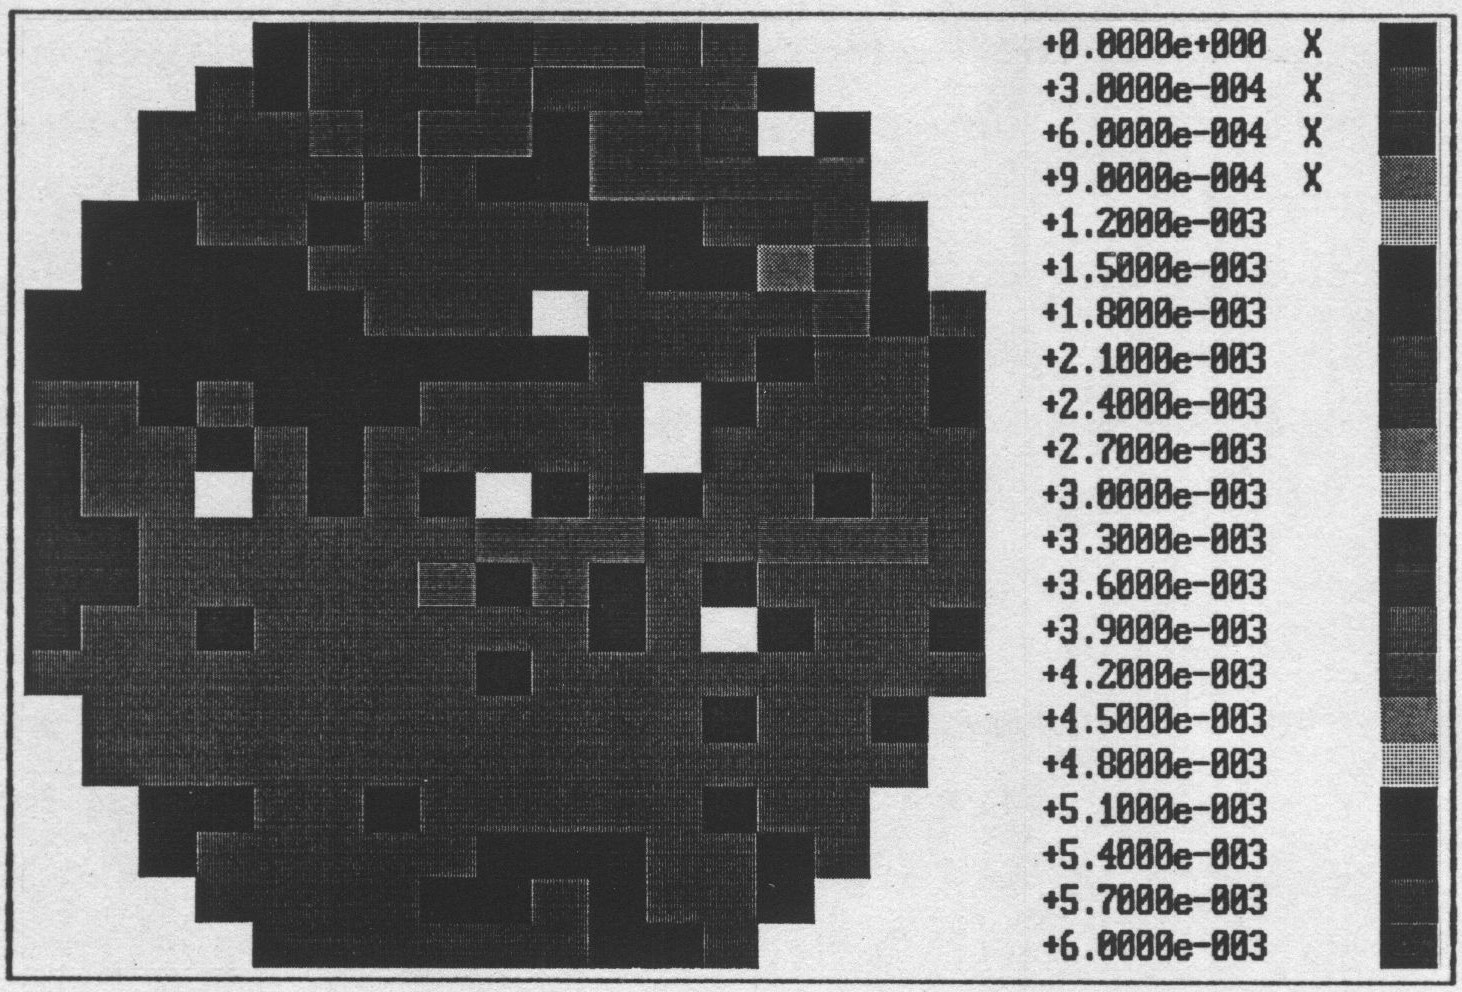
\includegraphics{Figures/fig-6-6.eps}
\captionsetup{justification=raggedright, singlelinecheck=false}
\caption[Plošné rozloženie generačného času života minoritných nosičov
  náboja]{Plošné rozloženie generačného času života minoritných
  nosičov náboja pre oblasť polovodiča od $0.9 \mu m$ do $1.3
  \mu m$.}
\label{fig:6.6}
\end{figure}

\begin{thebibliography}{}
\bibitem[6.1]{6.1}
Ludwig R.: Methoden der Fehler und Ausgleichrechnung. VEB Berlin 1969. s.103.
\end{thebibliography}
 
% Chapter 7
\chapter{Experimentálne výsledky.}\label{Chapter7}
\lhead{Kapitola 7. \emph{Experimentálne výsledky}}

Záverečný experiment bol uskutočnený na štruktúrach MOS s nehomogénnym
hĺbkovým profilom dotujúcich prímesí, ktorý bol vytvorený procesom
iónovej implantácie s rôznymi dávkami v monokryštále kremíka typu N s
orientáciou [100].

Pred technologickým spracovaním bola otestovaná homogenita
špecifického odporu použitých kremíkových dosiek pomocou zariadenia
Prometrix OmniMap RS35, ktoré využíva štvorbodovú metódu pre určenie
povrchového špecifického odporu. V tabuľke~\ref{tab:7.1} sú uvedené
stredné hodnoty špecifického odporu $\overline\rho$ a smerodajnej
odchýlky $\delta\rho$ vyjadrenej absolútnou a relatívnou hodnotou.

\begin{table}[h!]\centering
  \begin{minipage}[c]{\myfiguresize}
    \begin{center}
      \begin{tabular}{c c c c c c c c}
        č. & $\overline\rho[\Omega cm]$ & $\delta\rho[\Omega cm]$ & $\delta\rho[\%]$ &
        č. & $\overline\rho[\Omega cm]$ & $\delta\rho[\Omega cm]$ & $\delta\rho[\%]$\\
        \hline% chktex-file 44
        1  & 4.3319 & 0.1223 & 2.822 & 11 & 4.5706 & 0.1658 & 3.627\\
        2  & 4.2733 & 0.1204 & 2.817 & 12 & 4.4762 & 0.1860 & 4.155\\
        3  & 5.1040 & 0.3405 & 6.671 & 13 & 4.3332 & 0.1265 & 2.290\\
        4  & 4.6276 & 0.2080 & 4.494 & 14 & 4.8422 & 0.3573 & 7.380\\
        5  & 4.7697 & 0.1824 & 3.824 & 15 & 4.5917 & 0.1741 & 3.791\\
        6  & 4.8007 & 0.2340 & 4.873 & 16 & 4.8134 & 0.2590 & 5.380\\
        7  & 4.2500 & 0.1436 & 3.378 & 17 & 4.4025 & 0.1527 & 3.468\\
        8  & 4.8259 & 0.3163 & 6.554 & 18 & 4.3591 & 0.1290 & 2.960\\
        9  & 4.2853 & 0.1418 & 3.308 & 19 & 4.3877 & 0.1349 & 3.074\\
        10 & 4.2954 & 0.1113 & 2.592 & 20 & 4.5416 & 0.1618 & 3.563\\
      \end{tabular}
    \end{center}
    \caption[Stredná hodnota a smerodajná odchýlka špecifického odporu
      testovaných kremíkových dosiek pred technologickým
      spracovaním]{Stredná hodnota a smerodajná odchýlka špecifického
      odporu testovaných kremíkových dosiek pred technologickým
      spracovaním.}\label{tab:7.1}
  \end{minipage}
\end{table}

Zariadenie Prometrix OmniMap RS35 zmeralo pomocou krokovacieho
zariadenia hodnotu špecifického odporu v 81 bodoch každej dosky. Na
obrázku~\ref{fig:7.1} a obrázku~\ref{fig:7.2} uvádzame grafické
znázornenie rozloženia špecifického odporu, ktoré je taktiež výstupom
merania uvedeného zariadenia. Body, v ktorých bol zmeraný špecifický
odpor sú na obrázku~\ref{fig:7.1} vyznačené znakmi $+$, alebo $-$
podľa toho, či hodnota špecifického odporu v tomto bode ležala nad,
alebo pod strednou hodnotou, ktorá je znázornená hrubšou čiarou.
Predstavu o kvantitatívnom rozložení špecifického odporu si možno
urobiť z trojdimenzionálneho obrázku~\ref{fig:7.2}.

Postup hlavných technologických operácií vytvorenia štruktúr MOS na
uvedených substrátoch bol následovný

\begin{itemize}
\item vytvorenie hradlového oxidu s hrúbkou $100 \nu m$
\item implantácia $P^{31}$ s energiou $120 keV$ a dávkami 0.6, 1.0,
  2.0, 4.0, 5.0, 6.0, 7.0, 8.0, 20.0, 60.0 $\times 10^{15} m^{-2}$ pod
  uhlom $7\degree$
\item aktivácia pri teplote $1050 \degree C$ s časovým priebehom: 15
  min.\ nábeh, 30 min.\ aktivácia, 40 min.\ chladenie
\item naparenie Al na obe strany kremíkovej dosky
\item litografický proces vytvorenia CV masky
\item sintrovanie Al FG pri teplote $460 \degree C$ počas 20 min.
\end{itemize}

Uvedeným spôsobom bolo pripravených 20 kremíkových dosiek o priemere 4
palce, vždy dve s rovnakou dávkou implantácie.  V procese zberu dát
bolo na každej kremíkovej doske testovaných 304 štruktúr, pričom
plocha jednej štruktúry bola $0.81 \times 10^{-6} m^{-2}$. Na
obrázku~\ref{fig:7.3} sú znázornené priebehy koncentračných profilov
dotujúcich prímesi pre jednotlivé dávky implantácie. Znázornené
priebehy predstavujú strednú hodnotu cez všetky závislosti $N(x)$,
ktoré boli určené na testovanej doske. Z každej dávky je na
obrázku~\ref{fig:7.3} zobrazená len jedna kremíková doska.

\newpage
\begin{figure}[h!]\centering
  \begin{minipage}[c]{\myfiguresize}
    \begin{center}
      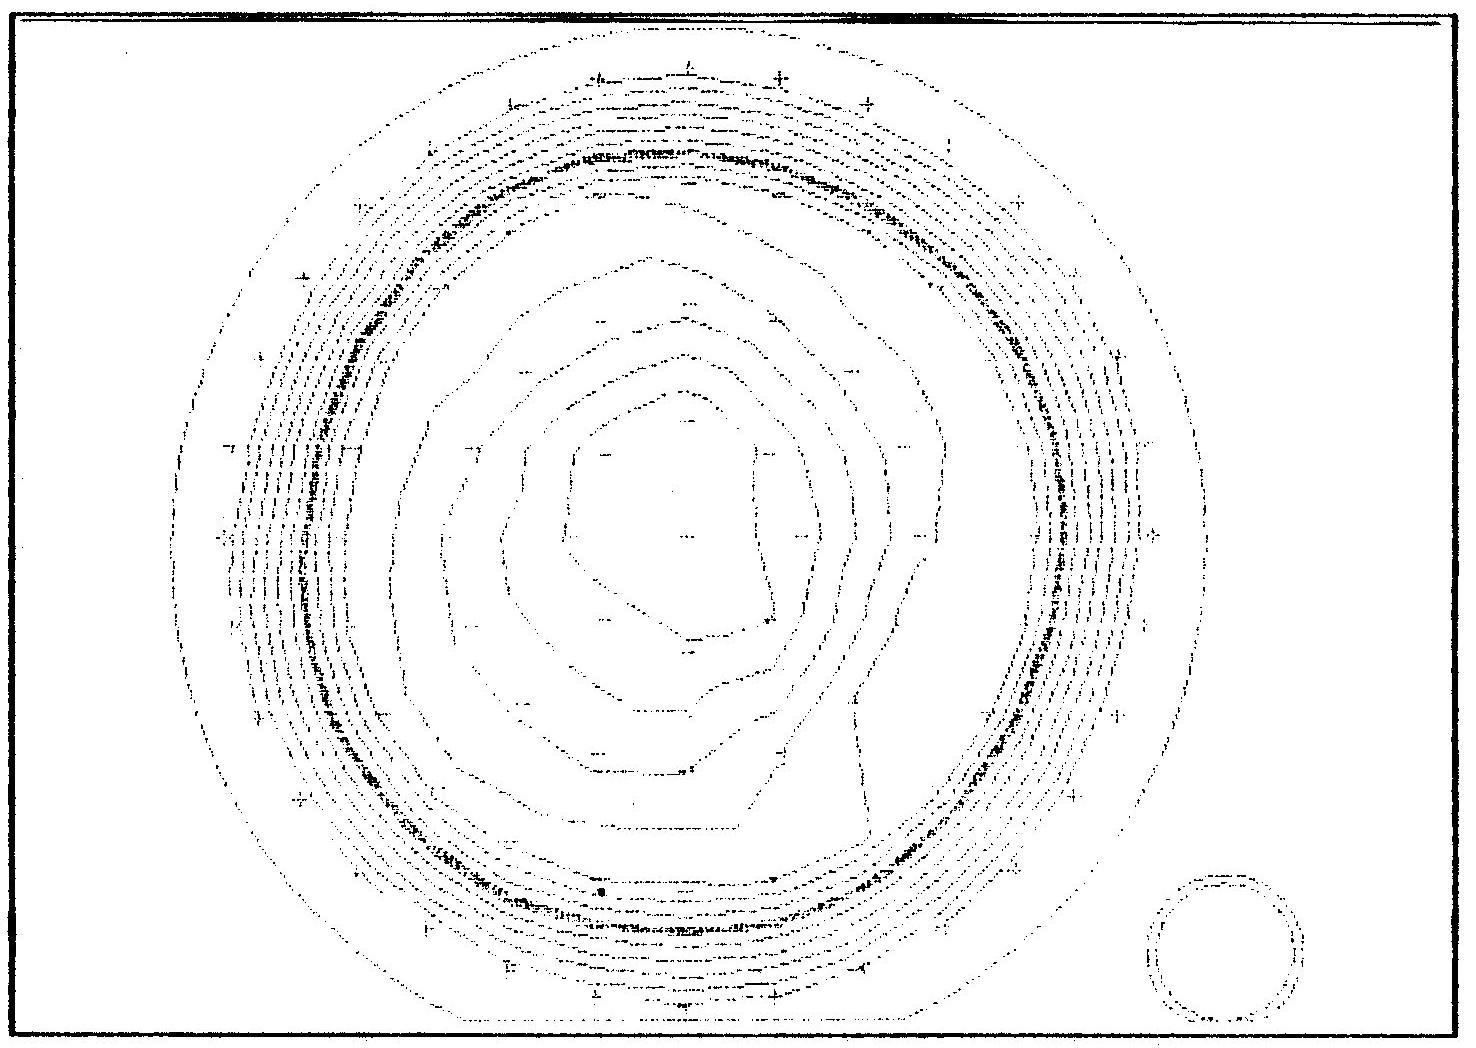
\includegraphics{Figures/fig-7-1.eps}% chktex-file 8
    \end{center}
    \caption[Plošné rozloženie povrchového špecifického odporu
      kremíkovej dosky č.16]{Plošné rozloženie povrchového
      špecifického odporu kremíkovej dosky č.16.}\label{fig:7.1}
  \end{minipage}
\end{figure}

\begin{figure}[h!]\centering
  \begin{minipage}[c]{\myfiguresize}
    \begin{center}
      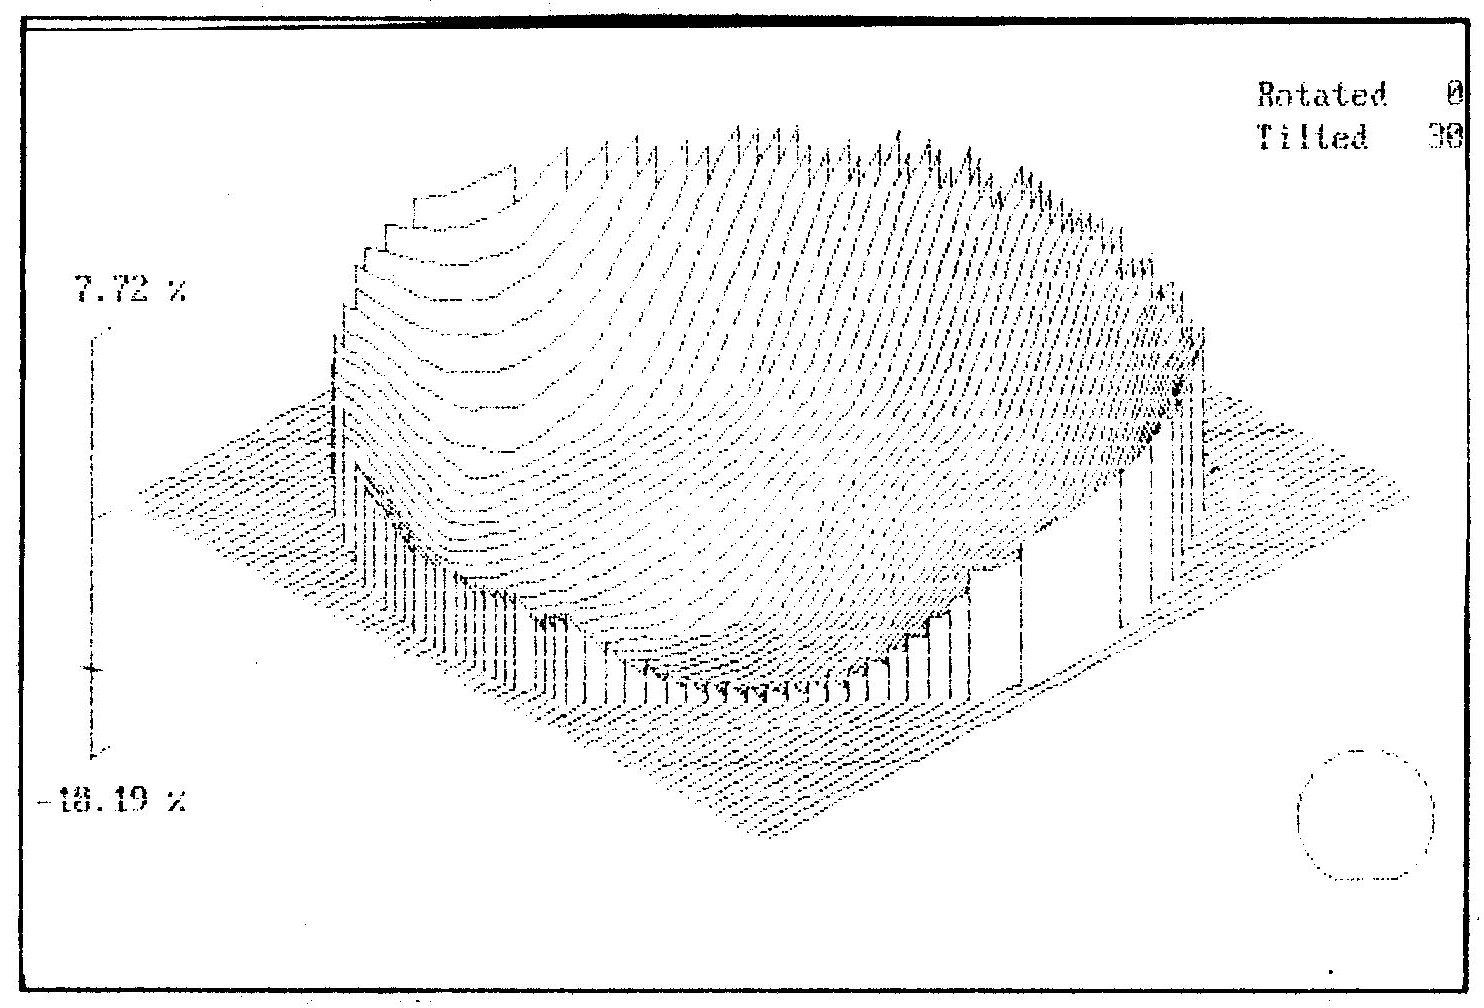
\includegraphics{Figures/fig-7-2.eps}
    \end{center}
    \caption[Plošné rozloženie povrchového špecifického odporu
      kremíkovej dosky č.16]{Plošné rozloženie povrchového
      špecifického odporu kremíkovej dosky č.16.}\label{fig:7.2}
  \end{minipage}
\end{figure}

\newpage
\begin{figure}[h!]\centering
  \begin{minipage}[c]{\myfiguresize}
    \begin{center}
      % GNUPLOT: LaTeX picture with Postscript
\begingroup
  \makeatletter
  \providecommand\color[2][]{%
    \GenericError{(gnuplot) \space\space\space\@spaces}{%
      Package color not loaded in conjunction with
      terminal option `colourtext'%
    }{See the gnuplot documentation for explanation.%
    }{Either use 'blacktext' in gnuplot or load the package
      color.sty in LaTeX.}%
    \renewcommand\color[2][]{}%
  }%
  \providecommand\includegraphics[2][]{%
    \GenericError{(gnuplot) \space\space\space\@spaces}{%
      Package graphicx or graphics not loaded%
    }{See the gnuplot documentation for explanation.%
    }{The gnuplot epslatex terminal needs graphicx.sty or graphics.sty.}%
    \renewcommand\includegraphics[2][]{}%
  }%
  \providecommand\rotatebox[2]{#2}%
  \@ifundefined{ifGPcolor}{%
    \newif\ifGPcolor
    \GPcolortrue
  }{}%
  \@ifundefined{ifGPblacktext}{%
    \newif\ifGPblacktext
    \GPblacktexttrue
  }{}%
  % define a \g@addto@macro without @ in the name:
  \let\gplgaddtomacro\g@addto@macro
  % define empty templates for all commands taking text:
  \gdef\gplbacktext{}%
  \gdef\gplfronttext{}%
  \makeatother
  \ifGPblacktext
    % no textcolor at all
    \def\colorrgb#1{}%
    \def\colorgray#1{}%
  \else
    % gray or color?
    \ifGPcolor
      \def\colorrgb#1{\color[rgb]{#1}}%
      \def\colorgray#1{\color[gray]{#1}}%
      \expandafter\def\csname LTw\endcsname{\color{white}}%
      \expandafter\def\csname LTb\endcsname{\color{black}}%
      \expandafter\def\csname LTa\endcsname{\color{black}}%
      \expandafter\def\csname LT0\endcsname{\color[rgb]{1,0,0}}%
      \expandafter\def\csname LT1\endcsname{\color[rgb]{0,1,0}}%
      \expandafter\def\csname LT2\endcsname{\color[rgb]{0,0,1}}%
      \expandafter\def\csname LT3\endcsname{\color[rgb]{1,0,1}}%
      \expandafter\def\csname LT4\endcsname{\color[rgb]{0,1,1}}%
      \expandafter\def\csname LT5\endcsname{\color[rgb]{1,1,0}}%
      \expandafter\def\csname LT6\endcsname{\color[rgb]{0,0,0}}%
      \expandafter\def\csname LT7\endcsname{\color[rgb]{1,0.3,0}}%
      \expandafter\def\csname LT8\endcsname{\color[rgb]{0.5,0.5,0.5}}%
    \else
      % gray
      \def\colorrgb#1{\color{black}}%
      \def\colorgray#1{\color[gray]{#1}}%
      \expandafter\def\csname LTw\endcsname{\color{white}}%
      \expandafter\def\csname LTb\endcsname{\color{black}}%
      \expandafter\def\csname LTa\endcsname{\color{black}}%
      \expandafter\def\csname LT0\endcsname{\color{black}}%
      \expandafter\def\csname LT1\endcsname{\color{black}}%
      \expandafter\def\csname LT2\endcsname{\color{black}}%
      \expandafter\def\csname LT3\endcsname{\color{black}}%
      \expandafter\def\csname LT4\endcsname{\color{black}}%
      \expandafter\def\csname LT5\endcsname{\color{black}}%
      \expandafter\def\csname LT6\endcsname{\color{black}}%
      \expandafter\def\csname LT7\endcsname{\color{black}}%
      \expandafter\def\csname LT8\endcsname{\color{black}}%
    \fi
  \fi
    \setlength{\unitlength}{0.0500bp}%
    \ifx\gptboxheight\undefined%
      \newlength{\gptboxheight}%
      \newlength{\gptboxwidth}%
      \newsavebox{\gptboxtext}%
    \fi%
    \setlength{\fboxrule}{0.5pt}%
    \setlength{\fboxsep}{1pt}%
\begin{picture}(7920.00,5616.00)%
    \gplgaddtomacro\gplbacktext{%
      \csname LTb\endcsname%%
      \put(1100,640){\makebox(0,0)[r]{\strut{}$1\times10^{21}$}}%
      \put(1100,2261){\makebox(0,0)[r]{\strut{}$1\times10^{22}$}}%
      \put(1100,3882){\makebox(0,0)[r]{\strut{}$1\times10^{23}$}}%
      \put(1220,440){\makebox(0,0){\strut{}$0$}}%
      \put(2012,440){\makebox(0,0){\strut{}$0.1$}}%
      \put(2805,440){\makebox(0,0){\strut{}$0.2$}}%
      \put(3597,440){\makebox(0,0){\strut{}$0.3$}}%
      \put(4390,440){\makebox(0,0){\strut{}$0.4$}}%
      \put(5182,440){\makebox(0,0){\strut{}$0.5$}}%
      \put(5974,440){\makebox(0,0){\strut{}$0.6$}}%
      \put(6767,440){\makebox(0,0){\strut{}$0.7$}}%
      \put(7559,440){\makebox(0,0){\strut{}$0.8$}}%
    }%
    \gplgaddtomacro\gplfronttext{%
      \csname LTb\endcsname%%
      \put(190,2827){\rotatebox{-270}{\makebox(0,0){\strut{}Koncentrácia $[{m}^{-3}]$}}}%
      \put(4389,140){\makebox(0,0){\strut{}Hĺbka $[\mu{m}]$}}%
      \put(4389,5315){\makebox(0,0){\strut{}Kocentrácia dopantov}}%
    }%
    \gplbacktext
    \put(0,0){\includegraphics{/export/scratch/vbotka-thesis/Plot/Figures/fig-7-3-sk}}%
    \gplfronttext
  \end{picture}%
\endgroup

    \end{center}
    \caption[Hĺbkový profil dotujúcich prímesí]{Hĺbkový profil
      dotujúcich prímesí v podpovrchovej oblasti polovodiča vytvorený
      iónovou implantáciou s dávkami $0.6, 1.0, 2.0, 4.0, 5.0, 6.0,
      7.0, 8.0, 20.0, 60.0 \times 10^{15} m^{-2}$. Zobrazené priebehy
      $N(x)$ predstavujú strednú hodnotu z priebehov, nameraných na
      304 štruktúrach MOS každej kremíkovej dosky.}\label{fig:7.3}
  \end{minipage}
\end{figure}
% OBR27.BIT

\newpage
\begin{figure}[h!]
  \begin{minipage}[c]{\myfiguresize}
    \begin{center}
      % GNUPLOT: LaTeX picture with Postscript
\begingroup
  \makeatletter
  \providecommand\color[2][]{%
    \GenericError{(gnuplot) \space\space\space\@spaces}{%
      Package color not loaded in conjunction with
      terminal option `colourtext'%
    }{See the gnuplot documentation for explanation.%
    }{Either use 'blacktext' in gnuplot or load the package
      color.sty in LaTeX.}%
    \renewcommand\color[2][]{}%
  }%
  \providecommand\includegraphics[2][]{%
    \GenericError{(gnuplot) \space\space\space\@spaces}{%
      Package graphicx or graphics not loaded%
    }{See the gnuplot documentation for explanation.%
    }{The gnuplot epslatex terminal needs graphicx.sty or graphics.sty.}%
    \renewcommand\includegraphics[2][]{}%
  }%
  \providecommand\rotatebox[2]{#2}%
  \@ifundefined{ifGPcolor}{%
    \newif\ifGPcolor
    \GPcolortrue
  }{}%
  \@ifundefined{ifGPblacktext}{%
    \newif\ifGPblacktext
    \GPblacktexttrue
  }{}%
  % define a \g@addto@macro without @ in the name:
  \let\gplgaddtomacro\g@addto@macro
  % define empty templates for all commands taking text:
  \gdef\gplbacktext{}%
  \gdef\gplfronttext{}%
  \makeatother
  \ifGPblacktext
    % no textcolor at all
    \def\colorrgb#1{}%
    \def\colorgray#1{}%
  \else
    % gray or color?
    \ifGPcolor
      \def\colorrgb#1{\color[rgb]{#1}}%
      \def\colorgray#1{\color[gray]{#1}}%
      \expandafter\def\csname LTw\endcsname{\color{white}}%
      \expandafter\def\csname LTb\endcsname{\color{black}}%
      \expandafter\def\csname LTa\endcsname{\color{black}}%
      \expandafter\def\csname LT0\endcsname{\color[rgb]{1,0,0}}%
      \expandafter\def\csname LT1\endcsname{\color[rgb]{0,1,0}}%
      \expandafter\def\csname LT2\endcsname{\color[rgb]{0,0,1}}%
      \expandafter\def\csname LT3\endcsname{\color[rgb]{1,0,1}}%
      \expandafter\def\csname LT4\endcsname{\color[rgb]{0,1,1}}%
      \expandafter\def\csname LT5\endcsname{\color[rgb]{1,1,0}}%
      \expandafter\def\csname LT6\endcsname{\color[rgb]{0,0,0}}%
      \expandafter\def\csname LT7\endcsname{\color[rgb]{1,0.3,0}}%
      \expandafter\def\csname LT8\endcsname{\color[rgb]{0.5,0.5,0.5}}%
    \else
      % gray
      \def\colorrgb#1{\color{black}}%
      \def\colorgray#1{\color[gray]{#1}}%
      \expandafter\def\csname LTw\endcsname{\color{white}}%
      \expandafter\def\csname LTb\endcsname{\color{black}}%
      \expandafter\def\csname LTa\endcsname{\color{black}}%
      \expandafter\def\csname LT0\endcsname{\color{black}}%
      \expandafter\def\csname LT1\endcsname{\color{black}}%
      \expandafter\def\csname LT2\endcsname{\color{black}}%
      \expandafter\def\csname LT3\endcsname{\color{black}}%
      \expandafter\def\csname LT4\endcsname{\color{black}}%
      \expandafter\def\csname LT5\endcsname{\color{black}}%
      \expandafter\def\csname LT6\endcsname{\color{black}}%
      \expandafter\def\csname LT7\endcsname{\color{black}}%
      \expandafter\def\csname LT8\endcsname{\color{black}}%
    \fi
  \fi
    \setlength{\unitlength}{0.0500bp}%
    \ifx\gptboxheight\undefined%
      \newlength{\gptboxheight}%
      \newlength{\gptboxwidth}%
      \newsavebox{\gptboxtext}%
    \fi%
    \setlength{\fboxrule}{0.5pt}%
    \setlength{\fboxsep}{1pt}%
\begin{picture}(7920.00,5616.00)%
    \gplgaddtomacro\gplbacktext{%
      \csname LTb\endcsname%%
      \put(740,640){\makebox(0,0)[r]{\strut{}$0.1$}}%
      \put(740,2215){\makebox(0,0)[r]{\strut{}$1$}}%
      \put(740,3790){\makebox(0,0)[r]{\strut{}$10$}}%
      \put(860,440){\makebox(0,0){\strut{}$0.1$}}%
      \put(3168,440){\makebox(0,0){\strut{}$1$}}%
      \put(5475,440){\makebox(0,0){\strut{}$10$}}%
    }%
    \gplgaddtomacro\gplfronttext{%
      \csname LTb\endcsname%%
      \put(190,2827){\rotatebox{-270}{\makebox(0,0){\strut{}Aktivované ióny ${10}^{15}[{m}^{-2}]$}}}%
      \put(4209,140){\makebox(0,0){\strut{}Implantačná dávka $D_{i}{10}^{15}[{m}^{-2}]$}}%
      \put(4209,5315){\makebox(0,0){\strut{}Aktivácia dopantov}}%
    }%
    \gplgaddtomacro\gplbacktext{%
      \csname LTb\endcsname%%
      \put(740,640){\makebox(0,0)[r]{\strut{}$0.1$}}%
      \put(740,2215){\makebox(0,0)[r]{\strut{}$1$}}%
      \put(740,3790){\makebox(0,0)[r]{\strut{}$10$}}%
      \put(860,440){\makebox(0,0){\strut{}$0.1$}}%
      \put(3168,440){\makebox(0,0){\strut{}$1$}}%
      \put(5475,440){\makebox(0,0){\strut{}$10$}}%
    }%
    \gplgaddtomacro\gplfronttext{%
      \csname LTb\endcsname%%
      \put(190,2827){\rotatebox{-270}{\makebox(0,0){\strut{}Aktivované ióny ${10}^{15}[{m}^{-2}]$}}}%
      \put(4209,140){\makebox(0,0){\strut{}Implantačná dávka $D_{i}{10}^{15}[{m}^{-2}]$}}%
      \put(4209,5315){\makebox(0,0){\strut{}Aktivácia dopantov}}%
    }%
    \gplbacktext
    \put(0,0){\includegraphics{/export/scratch/vbotka-thesis/Plot/Figures/fig-7-4-sk}}%
    \gplfronttext
  \end{picture}%
\endgroup

    \end{center}
    \caption[Závislosť strednej hodnoty
      $\overline{D}=E(\int(N(x)-N_{b})dx)$ od dávky implantovaných
      iónov $D_{i}$]{Závislosť strednej hodnoty
      $\overline{D}=E(\int(N(x)-N_{b})dx)$ od dávky implantovaných
      iónov $D_{i}$. Dáta z Tabuľky~\ref{tab:7.2}.}\label{fig:7.4}
  \end{minipage}
\end{figure}
%OBR29.BIT

Tabuľka~\ref{tab:7.2} obsahuje číselné hodnoty implantačnej dávky
zadané v procese implantácie $D_{i}$, strednú hodnotu $\overline D$ a
smerodajnú odchýlku $\delta D$ dávok vypočítaných postupom uvedeným v
časti~\ref{sec:6.1}.

\begin{table}[h!]\centering
  \begin{minipage}[c]{\myfiguresize}
    \begin{center}
      \begin{tabular}{c c c c}
        č. & ${D_{i}}{10}^{15}[m^{-2}]$ & $\overline{D}{10}^{15}[m^{-2}]$ & $\delta{D}{10}^{15}[m^{-2}]$\\
        \hline
         1 &  0.6 &  0.39 &  0.02\\
         3 &  1.0 &  0.59 &  0.08\\
         5 &  2.0 &  1.20 &  0.06\\
         7 &  4.0 &  2.67 &  0.09\\
         9 &  5.0 &  3.40 &  0.13\\
        11 &  6.0 &  4.07 &  0.13\\
        13 &  7.0 &  4.72 &  0.14\\
        15 &  8.0 &  5.49 &  0.09\\
        17 & 20.0 & 14.41 &  0.35\\
        19 & 60.0 & 42.63 &  0.21\\
      \end{tabular}
    \end{center}
    \caption[Dávky implantácie $D_{i}$]{Dávka implantácie $D_{i}$,
      vypočítaná stredná hodnota dávky implantovaných a aktivovaných
      iónov v polovodiči $\overline D$ a jej smerodajná odchýlka
      $\delta D$ na kremíkovej doske.}\label{tab:7.2}
  \end{minipage}
\end{table}

Pre kontrolu reprodukovateľnosti procesu implantácie boli zmerané
koncentračné profily na ďalších 3 kremíkových doskách.  V
tabuľke~\ref{tab:7.3} sa nachádzajú hodnoty dávok implantácie pre tri
dvojice kremíkových dosiek, ktoré boli implantované s tou istou
dávkou.

\begin{table}[h!]\centering
  \begin{minipage}[c]{\myfiguresize}
    \begin{center}
      \begin{tabular}{c c c c}
        č. & $D_{i} 10^{15} [m^{-2}]$ & $\overline D 10^{15} [m^{-2}]$ & $\delta D 10^{15} [m^{-2}]$\\
        \hline
         9 & 5.0 & 3.40 & 0.13\\
        10 & 5.0 & 3.56 & 0.06\\
        11 & 6.0 & 4.07 & 0.13\\
        12 & 6.0 & 4.03 & 0.12\\
        15 & 8.0 & 5.49 & 0.09\\
        16 & 8.0 & 5.46 & 0.08\\
      \end{tabular}
    \end{center}
    \caption[Dávka implantácie $D_{i}$]{Dávka implantácie $D_{i}$,
      vypočítaná stredná hodnota dávky implantovaných a aktivovaných
      iónov v polovodiči $\overline D$ a jej smerodajná odchýlka
      $\delta D$ na kremíkovej doske.}\label{tab:7.3}
  \end{minipage}
\end{table}

Ako je zrejmé z tabuľky~\ref{tab:7.2} a~\ref{tab:7.3}, vypočítaná
implantačná dávka je vždy menšia ako dávka zadaná v procese
implantácie. To je spôsobené jednako tým, že čas implantovaných iónov
je zachytená v oxidovej vrstve a jednako neúplnou aktiváciou
implantovaných iónov v polovodiči. Aby sme určili závislosť medzi
zadanou a vypočítanou dávkou, vypočítali sme lineárnou regresiou
koeficient $b$ vzťahu

\begin{equation}\label{eq:7.1}
  \overline D = bD_{i}
\end{equation}

ktorý mal hodnotu $b = 0.71$ a zároveň sme zobrazili závislosť
$\overline D = f(D_{i})$ na obrázku~\ref{fig:7.4}. Tým sme zistili, že
z pôvodnej dávky, ktorá bola implantovaná sa stalo elektricky
aktívnymi 71\% implantovaných iónov. Aby sme určili stupeň závislosti
medzi implantovanou dávkou a množstvom elektricky aktívnych prímesí v
polovodiči, ktoré boli implantované, vypočítali sme korelačný
koeficient medzi týmito veličinami. Použili sme vzťah

\begin{equation}\label{eq:7.2}
  R(X,Y) = \frac{E([X-E(X)][Y-E(Y)])}{D(X)D(Y)}
\end{equation}

,ktorý je uvedený napríklad v~\cite{7.1}. Vo vzťahu~\ref{eq:7.2} X a Y
predstavujú náhodné veličiny, E predstavuje strednú hodnotu a D
označuje smerodajnú odchýlku. Uvedeným spôsobom sme získali hodnotu
korelačného koeficientu

\centerline{$R(D_{i}, \overline{D}) = 0.99$}

pričom sme považovali hodnoty $D_{i}$ a $\overline{D}$ za realizácie
náhodnej veličiny a použili sme všetky hodnoty uvedené v
tabuľke~\ref{tab:7.2} a~\ref{tab:7.3}. Možno poznamenať, že v teórii
pravdepodobnosti je dokázaná veta, podľa ktorej $\rvert R(X,Y)\rvert =
1$ práve vtedy, keď s pravdepodobnosťou 1 platí

\centerline{$Y = a + b X$}

Z uvedeného vyplýva, že závislosť medzi hodnotami $D_{i}$ a $\overline
D$ je v tomto prípade lineárna.

Pomocou profesionálneho programu, zakúpeného Teslou Piešťany, na
simuláciu procesu iónovej implantácie boli vypočítané priebehy
koncentrácie prímesi pre dávky 0.6, 5.0 a 60.0 $\times10^{15}m^{-2}$.
Priebehy koncentračných profilov boli simulované na základe zadaných
podmienok implantácie, pričom sa použila metóda Pearson IV\@.
Porovnanie nameraných a simulovaných priebehov koncentrácie prímesí je
zobrazené na obrázku~\ref{fig:7.5}.

\begin{figure}[h!]\centering
  \begin{minipage}[c]{\myfiguresize}
    \begin{center}
      % GNUPLOT: LaTeX picture with Postscript
\begingroup
  \makeatletter
  \providecommand\color[2][]{%
    \GenericError{(gnuplot) \space\space\space\@spaces}{%
      Package color not loaded in conjunction with
      terminal option `colourtext'%
    }{See the gnuplot documentation for explanation.%
    }{Either use 'blacktext' in gnuplot or load the package
      color.sty in LaTeX.}%
    \renewcommand\color[2][]{}%
  }%
  \providecommand\includegraphics[2][]{%
    \GenericError{(gnuplot) \space\space\space\@spaces}{%
      Package graphicx or graphics not loaded%
    }{See the gnuplot documentation for explanation.%
    }{The gnuplot epslatex terminal needs graphicx.sty or graphics.sty.}%
    \renewcommand\includegraphics[2][]{}%
  }%
  \providecommand\rotatebox[2]{#2}%
  \@ifundefined{ifGPcolor}{%
    \newif\ifGPcolor
    \GPcolortrue
  }{}%
  \@ifundefined{ifGPblacktext}{%
    \newif\ifGPblacktext
    \GPblacktexttrue
  }{}%
  % define a \g@addto@macro without @ in the name:
  \let\gplgaddtomacro\g@addto@macro
  % define empty templates for all commands taking text:
  \gdef\gplbacktext{}%
  \gdef\gplfronttext{}%
  \makeatother
  \ifGPblacktext
    % no textcolor at all
    \def\colorrgb#1{}%
    \def\colorgray#1{}%
  \else
    % gray or color?
    \ifGPcolor
      \def\colorrgb#1{\color[rgb]{#1}}%
      \def\colorgray#1{\color[gray]{#1}}%
      \expandafter\def\csname LTw\endcsname{\color{white}}%
      \expandafter\def\csname LTb\endcsname{\color{black}}%
      \expandafter\def\csname LTa\endcsname{\color{black}}%
      \expandafter\def\csname LT0\endcsname{\color[rgb]{1,0,0}}%
      \expandafter\def\csname LT1\endcsname{\color[rgb]{0,1,0}}%
      \expandafter\def\csname LT2\endcsname{\color[rgb]{0,0,1}}%
      \expandafter\def\csname LT3\endcsname{\color[rgb]{1,0,1}}%
      \expandafter\def\csname LT4\endcsname{\color[rgb]{0,1,1}}%
      \expandafter\def\csname LT5\endcsname{\color[rgb]{1,1,0}}%
      \expandafter\def\csname LT6\endcsname{\color[rgb]{0,0,0}}%
      \expandafter\def\csname LT7\endcsname{\color[rgb]{1,0.3,0}}%
      \expandafter\def\csname LT8\endcsname{\color[rgb]{0.5,0.5,0.5}}%
    \else
      % gray
      \def\colorrgb#1{\color{black}}%
      \def\colorgray#1{\color[gray]{#1}}%
      \expandafter\def\csname LTw\endcsname{\color{white}}%
      \expandafter\def\csname LTb\endcsname{\color{black}}%
      \expandafter\def\csname LTa\endcsname{\color{black}}%
      \expandafter\def\csname LT0\endcsname{\color{black}}%
      \expandafter\def\csname LT1\endcsname{\color{black}}%
      \expandafter\def\csname LT2\endcsname{\color{black}}%
      \expandafter\def\csname LT3\endcsname{\color{black}}%
      \expandafter\def\csname LT4\endcsname{\color{black}}%
      \expandafter\def\csname LT5\endcsname{\color{black}}%
      \expandafter\def\csname LT6\endcsname{\color{black}}%
      \expandafter\def\csname LT7\endcsname{\color{black}}%
      \expandafter\def\csname LT8\endcsname{\color{black}}%
    \fi
  \fi
    \setlength{\unitlength}{0.0500bp}%
    \ifx\gptboxheight\undefined%
      \newlength{\gptboxheight}%
      \newlength{\gptboxwidth}%
      \newsavebox{\gptboxtext}%
    \fi%
    \setlength{\fboxrule}{0.5pt}%
    \setlength{\fboxsep}{1pt}%
\begin{picture}(7920.00,5616.00)%
    \gplgaddtomacro\gplbacktext{%
      \csname LTb\endcsname%%
      \put(1100,640){\makebox(0,0)[r]{\strut{}$1\times10^{21}$}}%
      \put(1100,2261){\makebox(0,0)[r]{\strut{}$1\times10^{22}$}}%
      \put(1100,3882){\makebox(0,0)[r]{\strut{}$1\times10^{23}$}}%
      \put(1220,440){\makebox(0,0){\strut{}$0$}}%
      \put(2012,440){\makebox(0,0){\strut{}$0.1$}}%
      \put(2805,440){\makebox(0,0){\strut{}$0.2$}}%
      \put(3597,440){\makebox(0,0){\strut{}$0.3$}}%
      \put(4390,440){\makebox(0,0){\strut{}$0.4$}}%
      \put(5182,440){\makebox(0,0){\strut{}$0.5$}}%
      \put(5974,440){\makebox(0,0){\strut{}$0.6$}}%
      \put(6767,440){\makebox(0,0){\strut{}$0.7$}}%
      \put(7559,440){\makebox(0,0){\strut{}$0.8$}}%
    }%
    \gplgaddtomacro\gplfronttext{%
      \csname LTb\endcsname%%
      \put(190,2827){\rotatebox{-270}{\makebox(0,0){\strut{}Koncentrácia $[{m}^{-3}]$}}}%
      \put(4389,140){\makebox(0,0){\strut{}Hĺbka $[\mu{m}]$}}%
      \put(4389,5315){\makebox(0,0){\strut{}Provnanie nameraných a simulovaných kocentrácií dopantov.}}%
    }%
    \gplbacktext
    \put(0,0){\includegraphics{/export/scratch/vbotka-thesis/Plot/Figures/fig-7-5-sk}}%
    \gplfronttext
  \end{picture}%
\endgroup

    \end{center}
    \caption[Porovnanie stredných hodnôt nameraných priebehov $N(x)$ a
      simulovaných pomocou metódy Pearson IV]{Porovnanie stredných
      hodnôt nameraných priebehov $N(x)$ a simulovaných pomocou metódy
      Pearson IV pre dávky $0.6, 5.0, 60.0 \times 10^{15}
      m^{-2}$. Namerané hodnoty ukazujú nižšiu
      koncentráciu.}\label{fig:7.5}
  \end{minipage}
\end{figure}
% OBR33.BIT

V procese výpočtu hĺbkových profilov dotujúcich prímesí sme zároveň
určili aj hodnoty napätia vyrovnaných pásov $V_{fb}$ pre každú
testovanú štruktúru MOS\@. Pomocou samostatného programu, ktorý určuje
na základe dát, nachádzajúcich sa v zadanom dátovom súbore strednú
hodnotu a smerodajnú odchýlku uložených parametrov, sme vypočítali
strednú hodnotu $\overline V{fb}$ a smerodajnú odchýlku $\delta
V{fb}$. Zároveň sme pomocou toho istého postupu určili hodnoty
$\overline h_{ox}$ a $\delta h_{ox}$, ktoré sú pre jednotlivé
kremíkové dosky uvedené v tabuľke~\ref{tab:7.4}. Z
tabuľky~\ref{tab:7.4} je vidieť, že hodnoty $\overline V_{fb}$ súvisia
so strednými hodnotami hrúbky oxidovej vrstvy $\overline h_{ox}$,
preto sme túto závislosť zobrazili na obrázku~\ref{fig:7.6}.

\newpage
\begin{figure}[h!]\centering
  \begin{minipage}[c]{\myfiguresize}
    \begin{center}
      % GNUPLOT: LaTeX picture with Postscript
\begingroup
  \makeatletter
  \providecommand\color[2][]{%
    \GenericError{(gnuplot) \space\space\space\@spaces}{%
      Package color not loaded in conjunction with
      terminal option `colourtext'%
    }{See the gnuplot documentation for explanation.%
    }{Either use 'blacktext' in gnuplot or load the package
      color.sty in LaTeX.}%
    \renewcommand\color[2][]{}%
  }%
  \providecommand\includegraphics[2][]{%
    \GenericError{(gnuplot) \space\space\space\@spaces}{%
      Package graphicx or graphics not loaded%
    }{See the gnuplot documentation for explanation.%
    }{The gnuplot epslatex terminal needs graphicx.sty or graphics.sty.}%
    \renewcommand\includegraphics[2][]{}%
  }%
  \providecommand\rotatebox[2]{#2}%
  \@ifundefined{ifGPcolor}{%
    \newif\ifGPcolor
    \GPcolortrue
  }{}%
  \@ifundefined{ifGPblacktext}{%
    \newif\ifGPblacktext
    \GPblacktexttrue
  }{}%
  % define a \g@addto@macro without @ in the name:
  \let\gplgaddtomacro\g@addto@macro
  % define empty templates for all commands taking text:
  \gdef\gplbacktext{}%
  \gdef\gplfronttext{}%
  \makeatother
  \ifGPblacktext
    % no textcolor at all
    \def\colorrgb#1{}%
    \def\colorgray#1{}%
  \else
    % gray or color?
    \ifGPcolor
      \def\colorrgb#1{\color[rgb]{#1}}%
      \def\colorgray#1{\color[gray]{#1}}%
      \expandafter\def\csname LTw\endcsname{\color{white}}%
      \expandafter\def\csname LTb\endcsname{\color{black}}%
      \expandafter\def\csname LTa\endcsname{\color{black}}%
      \expandafter\def\csname LT0\endcsname{\color[rgb]{1,0,0}}%
      \expandafter\def\csname LT1\endcsname{\color[rgb]{0,1,0}}%
      \expandafter\def\csname LT2\endcsname{\color[rgb]{0,0,1}}%
      \expandafter\def\csname LT3\endcsname{\color[rgb]{1,0,1}}%
      \expandafter\def\csname LT4\endcsname{\color[rgb]{0,1,1}}%
      \expandafter\def\csname LT5\endcsname{\color[rgb]{1,1,0}}%
      \expandafter\def\csname LT6\endcsname{\color[rgb]{0,0,0}}%
      \expandafter\def\csname LT7\endcsname{\color[rgb]{1,0.3,0}}%
      \expandafter\def\csname LT8\endcsname{\color[rgb]{0.5,0.5,0.5}}%
    \else
      % gray
      \def\colorrgb#1{\color{black}}%
      \def\colorgray#1{\color[gray]{#1}}%
      \expandafter\def\csname LTw\endcsname{\color{white}}%
      \expandafter\def\csname LTb\endcsname{\color{black}}%
      \expandafter\def\csname LTa\endcsname{\color{black}}%
      \expandafter\def\csname LT0\endcsname{\color{black}}%
      \expandafter\def\csname LT1\endcsname{\color{black}}%
      \expandafter\def\csname LT2\endcsname{\color{black}}%
      \expandafter\def\csname LT3\endcsname{\color{black}}%
      \expandafter\def\csname LT4\endcsname{\color{black}}%
      \expandafter\def\csname LT5\endcsname{\color{black}}%
      \expandafter\def\csname LT6\endcsname{\color{black}}%
      \expandafter\def\csname LT7\endcsname{\color{black}}%
      \expandafter\def\csname LT8\endcsname{\color{black}}%
    \fi
  \fi
    \setlength{\unitlength}{0.0500bp}%
    \ifx\gptboxheight\undefined%
      \newlength{\gptboxheight}%
      \newlength{\gptboxwidth}%
      \newsavebox{\gptboxtext}%
    \fi%
    \setlength{\fboxrule}{0.5pt}%
    \setlength{\fboxsep}{1pt}%
\begin{picture}(7920.00,5616.00)%
    \gplgaddtomacro\gplbacktext{%
      \csname LTb\endcsname%%
      \put(860,640){\makebox(0,0)[r]{\strut{}$-1.7$}}%
      \put(860,1369){\makebox(0,0)[r]{\strut{}$-1.6$}}%
      \put(860,2098){\makebox(0,0)[r]{\strut{}$-1.5$}}%
      \put(860,2828){\makebox(0,0)[r]{\strut{}$-1.4$}}%
      \put(860,3557){\makebox(0,0)[r]{\strut{}$-1.3$}}%
      \put(860,4286){\makebox(0,0)[r]{\strut{}$-1.2$}}%
      \put(860,5015){\makebox(0,0)[r]{\strut{}$-1.1$}}%
      \put(980,440){\makebox(0,0){\strut{}$92$}}%
      \put(1992,440){\makebox(0,0){\strut{}$94$}}%
      \put(3004,440){\makebox(0,0){\strut{}$96$}}%
      \put(4016,440){\makebox(0,0){\strut{}$98$}}%
      \put(5029,440){\makebox(0,0){\strut{}$100$}}%
      \put(6041,440){\makebox(0,0){\strut{}$102$}}%
      \put(7053,440){\makebox(0,0){\strut{}$104$}}%
    }%
    \gplgaddtomacro\gplfronttext{%
      \csname LTb\endcsname%%
      \put(190,2827){\rotatebox{-270}{\makebox(0,0){\strut{}Napätie vyrovnaných pásov $[V]$}}}%
      \put(4269,140){\makebox(0,0){\strut{}Hrúbka oxidu $[nm]$}}%
      \put(4269,5315){\makebox(0,0){\strut{}Napätie vyrovnaných pásov / Hrúbka oxidu}}%
    }%
    \gplbacktext
    \put(0,0){\includegraphics{/export/scratch/vbotka-thesis/Plot/Figures/fig-7-6-sk}}%
    \gplfronttext
  \end{picture}%
\endgroup

    \end{center}
    \caption[Závislosť strednej hodnoty $\overline V_{fb}$ od strednej
      hodnoty hrúbky oxidovej vrstvy $\overline h_{ox}$]{Závislosť
      strednej hodnoty napätia vyrovnaných pásov $\overline V_{fb}$ od
      strednej hodnoty hrúbky oxidovej vrstvy $\overline h_{ox}$ pre
      kremíkové dosky číslo 1, 3, 5, 7, 9, 11, 13, 15 a 17. Dáta z
      Tabuľky~\ref{tab:7.4}}\label{fig:7.6}
  \end{minipage}
\end{figure}
% OBR28.BIT

\begin{table}[h!]\centering
  \begin{minipage}[c]{\myfiguresize}
    \begin{center}
      \begin{tabular}{c c c c c}
        č. & $\overline V_{fb} [V]$ & $\delta V_{fb} [V]$ & $\overline h_{ox} [nm]$ & $\delta h_{ox} [nm]$\\ 
        \hline
         1 & -1.24 & 0.07 &  94.14 & 0.89\\
         3 & -1.43 & 0.07 &  97.79 & 0.80\\
         5 & -1.35 & 0.08 &  97.26 & 0.28\\
         7 & -1.40 & 0.09 &  98.15 & 0.35\\
         9 & -1.52 & 0.09 & 102.85 & 0.53\\
        11 & -1.48 & 0.08 & 101.65 & 0.32\\
        13 & -1.38 & 0.08 & 100.94 & 0.41\\
        15 & -1.33 & 0.07 & 100.80 & 0.16\\
        17 & -1.59 & 0.08 &  99.93 & 0.22\\
        19 & -2.43 & 0.16 &  99.67 & 0.19\\
      \end{tabular}
    \end{center}
    \caption[Stredná hodnota a smerodajná odchýlka napätia vyrovnaných
      pásov a hrúbky oxidu]{Stredná hodnota a smerodajná odchýlka
      napätia vyrovnaných pásov a hrúbky oxidu.}\label{tab:7.4}
  \end{minipage}
\end{table}

Hodnota korelačného koeficientu

\centerline{$R(\overline V_{fb} ,\overline h_{ox}) = -0.78$}

súhlasí s teoretickým vzťahom, určujúcim závislosť hodnoty $V_{fb}$ od
veľkosti poruchového náboja v oxidovej vrstve a na rozhraní
$Si-SiO_{2}$ $Q_{dc}$ a od veľkosti kapacity oxidovej vrstvy $C_{ox}$

\begin{equation}\label{eq:7.3}
  V_{fb}  = \varphi_{ms} + \frac{Q_{dc}}{C_{ox}}
\end{equation}

kde $\varphi_{ms}$ predstavuje rozdiel výstupných potenciálov medzi
polovodičom a kovom.

Pre koeficienty lineárnej regresie 

\centerline{$V_{fb}  = a + b h_{ox}$}

sme dostali hodnoty 

\centerline{$a = 5.48 \times 10^{-3}  \qquad  b = -1.41 \times 10^{7}$}

Na štyroch kremíkových doskách bola určená hustota pascí rozhrania
$Si-SiO_2$ $D_{it}$. Ako vidieť z tabuľky~\ref{tab:7.5}, stredné
hodnoty $\overline D_{it}$ sa pohybujú v oblasti $2.0-5.0\times
10^{14}$, čo hovorí o dobrej kvalite rozhrania $Si-SiO_{2}$.

O kvalite kryštálu podáva informáciu veľkosť generačného času
minoritných nosičov náboja. Aby sme mohli porovnať kvalitu kryštálu
pre jednotlivé dosky, určili sme na každej kremíkovej doske plošné
rozloženie $\tau_{g}$ v hĺbke od $0.9$ do $1.3\mu m$. Pre všetky dosky
sme potom určili strednú hodnotu $\overline\tau_{g}$ a smerodajnú
odchýlku $\delta\tau_{g}$, ktorých hodnoty sú uvedené v
tabuľke~\ref{tab:7.6}. Hodnoty $\overline\tau_{g}$ sa pohybujú v
rozmedzí $0.41 - 2.25 ms$, čo hovorí o vysokej kvalite
substrátu. Zároveň z tabuľky~\ref{tab:7.6} vidieť, že hodnoty
$\overline \tau_{g}$ sa pohybujú náhodne a nie je možné nájsť
závislosť od ďalších, predtým spomenutých parametrov.

\begin{table}[h!]\centering
  \begin{minipage}[c]{\myfiguresize}
    \begin{center}
      \begin{tabular}{c c c}
        č. & ${\bar{D_{it}}}[m^{-2}eV^{-1}]$ & $\delta D_{it}[m^{-2}eV^{-1}]$\\ 
        \hline
         3 & $4.42 \times 10^{14}$ & $0.25 \times 10^{14}$\\
         7 & $2.60 \times 10^{14}$ & $0.15 \times 10^{14}$\\
         9 & $2.74 \times 10^{14}$ & $0.15 \times 10^{14}$\\
        12 & $3.55 \times 10^{14}$ & $0.16 \times 10^{14}$\\
      \end{tabular}
    \end{center}
    \caption[Stredná hodnota a smerodajná odchýlka hustoty pascí
      rozhrania $Si-SiO_{2}$ v strede zakázaného pásma.]{Stredná
      hodnota a smerodajná odchýlka hustoty pascí rozhrania
      $Si-SiO_{2}$ v strede zakázaného pásma.}\label{tab:7.5}
  \end{minipage}
\end{table}

\begin{table}[h!]\centering
  \begin{minipage}[c]{\myfiguresize}
    \begin{center}
      \begin{tabular}{c c c}
        č. & ${\bar{\tau_{g}}}[ms]$ & $\delta\tau_{g}[ms]$\\ 
        \hline
         1 & 1.93 & 0.12\\
         3 & 1.48 & 0.09\\
         5 & 1.84 & 0.09\\
         7 & 1.67 & 0.10\\
        10 & 1.95 & 0.09\\
        12 & 0.41 & 0.02\\
        15 & 1.74 & 0.09\\
        17 & 2.25 & 0.14\\
      \end{tabular}
    \end{center}
   \caption[Stredná hodnota a smerodajná odchýlka generačnej doby
     života minoritných nosičov náboja]{Stredná hodnota a smerodajná
     odchýlka generačnej doby života minoritných nosičov
     náboja.}\label{tab:7.6}
  \end{minipage}
\end{table}


\begin{thebibliography}{}
\bibitem[7.1]{7.1}
  Renyi A.: Teorie pravdepodobnosti. Academia Praha 1972.
\end{thebibliography}
 
% Chapter 8
\chapter{Súhrn výsledkov s uvedením nových poznatkov.}
\label{Chapter8}
\lhead{Chapter 8. \emph{Súhrn výsledkov s uvedením nových poznatkov}}
% This is for the header on each page - perhaps a shortened title
%----------------------------------------------------------------------

V dizertačnej práci sú uvedené výsledky získané pri skúmaní parametrov
štruktúr MOS s nehomogénnym rozložením prímesí v podpovrchovej oblasti
polovodiča. Vzhľadom k tomu, že u nás nebola doposiaľ táto
problematika komplexne riešená, bolo potrebné zhrnúť súčasné poznatky
z tejto oblasti, zvládnuť metodiku merania a vyhodnotenia parametrov a
prakticky ich realizovať. Praktická stránka pozostávala z realizácie
jednotlivých kapacitných metód a vytvorenia komplexného pracoviska pre
meranie a vyhodnotenie plošného rozloženia parametrov štruktúr MOS s
perspektívou ďalšieho využitia pre skúmanie korelácií medzi
jednotlivými parametrami, prípadne medzi parametrami iných testovacích
štruktúr, alebo technologických postupov planárnej technológie.

Dizertačná práca priniesla následovné výsledky:

\begin{enumerate}

% 1
\item Vyriešili sme jedno-dimenzionálnu Poissonovu rovnicu pre
  nehomogénne dotovaný substrát polovodiča a vypočítali sme teoretické
  CV závislosti štruktúry MOS. Numerické riešenie Poissonovej rovnice
  umožnilo získať informácie o fyzikálnych dejoch v štruktúre MOS v
  procese merania CV závislostí a umožnilo overenie použitých
  aproximácií pri výpočte koncentračných profilov.

%2
\item Okrem Štandardnej vysokofrekvenčnej a kvázistatickej CV
  metódy sme realizovali postup merania štruktúr MOS metódou QC, kde
  bolo potrebné:

\begin{itemize}
\item navrhnúť a realizovať prípravok pre umiestnenie meranej vzorky a
  vzduchového kondenzátora
\item  minimalizovať zvodové prúdy a parazitné kapacity
\item zvoliť vhodné postupy určovania parazitných kapacít
\item vytvoriť programové vybavenie pre zber a spracovanie dát.
\end{itemize}

Ako sa ukázalo počas zavádzania metódy, ako aj počas následovných
experimentov, implementácia metódy QC vyžaduje vytvorenie dôkladného
meracieho pracoviska s dôrazom na minimalizáciu zvodových prúdov a
parazitných kapacít.

%3
\item Pre meranie generačného času života minoritných nosičov náboja
  sme implementovali metódu konštantnej šírky OPN (CCT), ktorá
  umožňuje efektívne vyhodnocovanie kvality polovodičových substrátov
  pre vysoké hodnoty $\tau_{g}$ . Pri tvorbe riadiaceho programu sme
  navrhli a realizovali algoritmus pre udržanie konštantnej
  nerovnovážnej kapacity štruktúry MOS a merania závislosti
  $V_{g}(t)$.

%4
\item Všetky použité metódy (HF, LF, QC a CCT) boli automatizované
  pomocou osobného počítača PC AT s interfejsom PCIIA, pričom bolo
  potrebné zvládnuť riadenie zbernice IMS-2 a efektívne využiť
  autonómne schopnosti použitých prístrojov. Pre skúmanie plošného
  rozloženia parametrov štruktúr MOS na kremíkovej doske sme
  vypracovali programový balík pozostávajúci z približne 40 programov,
  ktoré vykonávajú zber dát, ich spracovanie a určenie parametrov
  štruktúr MOS.  Zároveň sú k dispozícii programy pre zobrazenie
  získaných výsledkov.  Stručný prehľad vytvorených programov, ktoré
  slúžia pre zber, spracovanie a zobrazenie dát plošného rozloženia
  parametrov štruktúr MOS, je v dodatku \ref{app:AppendixH}.

%5
\item Pri výpočte koncentračných profilov dotujúcich prímesí v
  podpovrchovej oblasti polovodiča sme aplikovali:
\begin{itemize}
\item korekciu aproximácie hlbokého ochudobnenia pri povrchu
  polovodiča
\item korekciu vzhľadom na hustotu pascí rozhrania $Si-SiO_{2}$
\item výpočet šírky oblasti OPN pomocou aproximácie priebehu
  elektrického potenciálu v polovodiči
\item výpočet priestorového rozloženia dotujúcich atómov z
  koncentračného profilu majoritných nosičov náboja.
\end{itemize}

%6
\item Vhodnosť použitých aproximácií sme overili riešením Poissonovej
  rovnice a výpočtom koncentračného profilu majoritných nosičov náboja
  z teoretickej CV závislosti.  Tu sa ukázalo, že pre určovanie
  koncentračných profilov implantovaných prímesí testovaných
  kremíkových dosiek v záverečnom experimente je použitie uvedených
  aproximácii vhodné.

%7
\item Pre rôzne dávky implantácie v rozsahu od $0.6 \times 10^{15}$ do
  $60.0 \times 10^{15} m^{-2}$ sme určili na 10 kremíkových doskách
  priebehy koncentračných profilov $N(x)$ na približne 300 štruktúrach
  MOS každej testovanej dosky a vypočítali sme ich stredné
  hodnoty. Zároveň sme určili strednú hodnotu časti dávky
  implantovaných iónov, ktoré sa stali elektricky aktívnymi v
  polovodiči $D_{a}$ . Ukázalo sa, že závislosť medzi dávkou
  implantácie $D_{i}$ a množstvom elektricky aktívnych, implantovaných
  prímesí $D_{a}=f(D_{i})$ je lineárna, čo usudzujeme z hodnoty
  korelačného koeficientu $R(D_{i},D_{a})=0.99$.  Lineárnou regresiou
  závislosti $D_{a}=f(D_{i})$ sme zistili, že z pôvodnej implantovanej
  dávky sa do polovodiča dostalo a stalo sa elektricky aktívnymi
  $71\%$ iónov. Uvedenú metodiku možno využiť pri kontrole procesu
  implantácie a bola vypracovaná na základe požiadavky Tesly Piešťany.

%8
\item Vypočítané koncentračné profily sme overili simuláciou
  technologického procesu implantácie pomocou funkcie Pearson IV. Z
  porovnania výsledkov zistených pomocou kapacitných meraní a
  simulácie vidieť malý rozdiel, ktorý môže byť spôsobený tým, že v
  procese poimplantačného tepelného spracovania neboli všetky
  implantované ióny aktivované.  Zistené rozdiely sú však
  minimálne. Bola vypracovaná metodika na sledovanie plošného
  rozloženia hĺbkových profilov dotujúcich prímesí v rámci hraníc
  použiteľnosti kapacitnej metódy s možnosťou sledovať plošné
  rozloženie v ľubovolnej hĺbke pod povrchom polovodiča. Na základe
  experimentálnych výsledkov možno konštatovať, že proces implantácie
  prebiehal na 4 palcových kremíkových substrátoch reprodukovateľne s
  vysokou homogenitou rozloženia prímesí, čím sme overili kvalitu
  implantačného zariadenia.

%9
\item Predchádzajúce výsledky, získané pri určovaní hĺbkových
  koncentračných profilov, sa využili pri skúmaní vlastností rozhrania
  $Si-SiO_{2}$ štruktúr MOS s implantovaným substrátom. Pre analýzu
  týchto štruktúr bola použitá:
\begin{enumerate}
%a
\item diferenciálna kapacitná metóda, porovnávajúca HF a LF CV
  závislosť štruktúry MOS, pričom výpočet $\varphi_{s}(V_{g})$
  zohľadňuje hĺbkový profil prímesí
%b
\item kvázistatická CV metóda, založená na porovnaní experimentálnej a
  teoretickej CV závislosti.
\end{enumerate}
Z porovnania výsledkov získaných oboma metódami vyplýva, že hustota
pascí rozhrania $Si-SiO_{2}$ v strede zakázaného pásu sa prakticky
nelíši. Obe metodiky možno aplikovať na CV závislosti určené pomocou
HF a kvázistatickej metódy, alebo na CV závislosti štruktúry MOS
určené pomocou QC metódy. Zároveň sme zvládli postup určenia priebehu
povrchového potenciálu $\varphi_s(V_g)$ pomocou QC metódy, alebo
integráciou LF CV závislosti. Pre výpočet hustoty pascí z porovnania
experimentálnej a teoretickej CV závislosti sme použili teoretickú LF
CV závislosť určenú pomocou numerického riešenia Poissonovej rovnice
pre nehomogénne rozloženie dotujúcich prímesí v polovodiči.

%10
\item Z porovnania HF a LF CV závislosti sme určili plošné rozloženie
  hustoty pascí rozhrania $Si-SiO_{2}$ . Stredná hodnota hustoty pascí
  rozhrania v strede zakázaného pásu testovaných dosiek sa pohybovala
  v intervale od $2.6 \times 10^{14}$ do $4.4 \times 10^{14}
  m^{-2}eV^{-1}$. Tieto hodnoty sú na dolnej hranici rozlišovacej
  schopnosti použitej metódy a hovoria o dobrej kvalite rozhrania
  $Si-SiO_{2}$ testovaných vzoriek a súčasne o kvalite opracovania
  polovodičových substrátov.

%11
\item V záverečnom experimente sme metódou CCT určili plošné
  rozloženie strednej hodnoty $\tau_{g}$ na 8 kremíkových doskách v
  hĺbke od $0.9$ do $1.3 mm$, ktoré sa pohybujú od $0.41$ do $2.25
  ms$, čo hovorí o vysokej kvalite substrátu. \newline Výhodou
  použitej metódy je, že vyhodnocuje $\tau_{g}$ z generačného prúdu
  minoritných nosičov náboja len z oblasti OPN a eliminuje vplyv
  generácie minoritných nosičov náboja mimo túto oblasť, čo sa
  prejavilo na reprodukovateľnosti hodnôt tohto parametra. \newline
  Bola zistená vzájomná súvislosť medzi hĺbkovým profilom doby života
  a koncentračným profilom implantovaných prímesí.  Dosiahnuté
  výsledky poukazujú, že u skúmaných vzoriek dominantný mechanizmus,
  ktorý určuje dobu života je rozptyl na ionizovaných prímesiach. To
  taktiež potvrdzuje, že skúmané polovodičové substráty sú
  vysoko-kvalitné z hľadiska defektov a preto je rozptyl na nich
  vzhľadom na rozptyl na ionizovaných prímesiach zanedbateľný.

%12
\item Určili sme plošné rozloženie hrúbky oxidovej vrstvy vypočítanej
  z kapacity štruktúry MOS v akumulácii na 10 kremíkových doskách, z
  ktorého vidieť nehomogenity hrúbky $SiO_{2}$ spôsobené nerovnomerným
  rozložením teploty a turbulenciami oxidačnej atmosféry v trubici
  oxidačnej pece. \newline Stredné hodnoty hrúbky $SiO_{2}$ na jednotlivých
  doskách sa pohybujú v intervale od $94.14$ do $102.85 nm$, pričom
  v technologickom procese výroby štruktúr MOS bola požadovaná hodnota
  $100 nm$. \newline Zároveň je z tabuľky stredných hodnôt vidieť, že
  hrúbka oxidu je najnižšia pre kremíkové dosky, ktoré sa nachádzali
  na prednom a zadnom konci oxidačnej lodičky a najhrubší oxid sa
  vytvoril v strede, čo bolo spôsobené rozdelením teploty v oxidačnej
  trubici. Tieto poznatky sú v súlade s Bermannovým modelom mechanizmu
  termickej oxidácie.

%13
\item Skúmali sme plošné rozloženie napätia vyrovnaných pásov $V_{fb}$
  pre 10 kremíkových dosiek. Stredné hodnoty $V_{fb}$ na jednotlivých
  kremíkových doskách sa pohybujú v rozsahu od $-1.24$ do $-2.43
  V$. Vzhľadom k tomu, že náboj pascí rozhrania je pre skúmané dosky
  malý, rozptyl stredných hodnôt $V_{fb}$ môže byť spôsobený nábojom
  alkalických iónov v oxide.

%14
\item Pre riešenie rovníc matematickej fyziky sme použili metódy
  numerickej matematiky. Riešili sme diferenciálnu rovnicu druhého
  rádu s počiatočnými podmienkami pomocou metódy prediktor-korektor so
  štartovacím úsekom Runge-Kutta, hľadali sme korene nelineárnej
  rovnice metódou dotyčníc, použili sme číslicové filtre pre
  vyhladenie a určenie derivácií experimentálne získaných dát. Použili
  sme funkcie knižnice NAG pre aproximáciu kubickými splajn-funkciami.

%15
\item Vypracovali sme systém a štruktúry dátových súborov, ktoré
  uchovávajú namerané dáta a určené parametre štruktúry MOS, pričom
  sme zohľadnili vzťahy medzi jednotlivými metodikami merania a
  určovania parametrov, čo prispieva k väčšej efektívnosti programov a
  umožňuje ďalšie použitie získaných výsledkov.

\end{enumerate}
 
% Chapter 9
\chapter{Závery pre prax a rozvoj vednej disciplíny.}
\label{Chapter9}
\lhead{Chapter 9. \emph{Závery pre prax a rozvoj vednej disciplíny}}

Z hľadiska zvolených cieľov bolo dosiahnutých viacero poznatkov, ktoré
sa uplatnili v praxi pri kontrole technologických postupov vytvárania
polovodičových štruktúr planárnou technológiou. Záverom môžeme prínosy
práce zhrnúť do následovných bodov:

\begin{enumerate}

% 1
\item Realizácia komplexného automatizovaného pracoviska pre skúmanie
  elektro-fyzikálnych vlastností štruktúr MOS s nehomogénnym
  rozložením prímesí s možnosťou sledovania plošného rozloženia:
\begin{itemize}
\item koncentračného profilu dotujúcich prímesi $N(x)$ pre rôzne hĺbky
  $x$
\item hĺbkového profilu času života $\tau_{g}(x)$ pre rôzne hĺbky $x$
\item hustoty pascí rozhrania $Si-SiO_{2}$ $D_{it}(E_{c}-E)$ pre rôzne
  energie v zakázanom páse polovodiča
\item napätia vyrovnaných pásov $V_{fb}$
\item hrúbky oxidovej vrstvy $h_{ox}$.
\end{itemize}

% 2
\item Výber vhodných numerických metód a ich použitie pre riešenie:
\begin{itemize}

\item jednodimenzionálnej Poissonovej rovnice

\item nelineárnej rovnice pre určenie povrchového potenciálu z
  kapacity OPN $C_{sc}$
  
\item vyhladenia a interpolácie experimentálne určených dát

\item výpočet derivácie experimentálne určených dát.

\end{itemize}

% 3
\item Vytvorenie programového vybavenia pre riadenie experimentálnych
  meraní, spracovanie a zobrazenie výsledkov vybraných parametrov
  štruktúr MOS s nehomogénnym rozložením prímesí v podpovrchovej
  oblasti polovodiča a ich plošného rozloženia.

% 4
\item Skúmanie homogenity procesu implantácie na 4-palcových
  kremíkových doskách s rozsahom dávok od $0.6 \times 10^{14}$ do
  $60.0 \times 10^{14} m^{-2}$ vzhľadom na:
\begin{itemize}
\item hĺbkový profil aktívnych prímesí
\item vlastnosti rozhrania $Si-SiO_{2}$
\item hĺbkový profil generačného času života minoritných nosičov
  náboja.
\end{itemize}

% 5
\item Navrhla a realizovala sa metodika pre určenie implantovanej
  dávky prímesí. Experimentálne výsledky boli overené simuláciou
  technologického procesu pomocou funkcie Pearson IV. Porovnanie
  experimentálnych a teoretických výsledkov vykazujú minimálny
  rozdiel. Navrhnutá metodika kontroly implantovanej dávky je
  aplikovateľná v praxi.

% 6
\item Zistila sa vzájomná súvislosť medzi koncentračným profilom
  dotujúcich prímesí a hĺbkovým profilom generačného času života
  minoritných nosičov náboja. Profil času života kvalitných
  kremíkových substrátov nie je určený mechanizmom rozptylu na
  náhodných defektoch substrátu, ale len na implantovaných prímesiach.

\end{enumerate}
 

%----------------------------------------------------------------------------------------
%	THESIS CONTENT - APPENDICES
%----------------------------------------------------------------------------------------
\addtocontents{toc}{\vspace{2em}} % Add a gap in the Contents, for aesthetics
\appendix % Cue to tell LaTeX that the following 'chapters' are Appendices
% Include the appendices of the thesis as separate files from the Appendices folder
% Uncomment the lines as you write the Appendices
% Appendix A

\chapter{Numerické riešenie Poissonovej rovnice.}\label{app:AppendixA}
\raggedright\lhead{Dodatok A. \emph{Numerické riešenie Poissonovej rovnice}}

Poissonovu rovnicu možno napísať v normalizovanom tvare
(Dodatok~\ref{app:AppendixB})

\begin{equation}\label{eq:A.1}
  \frac{d^2u}{dx^2} = e^u - e^{2u_f-u} + \alpha(x) - 1 \qquad {x\ge0}
\end{equation}

 Koncentrácie majoritných a minoritných nosičov náboja predstavujú
 prvé dva členy na pravej strane rovnice. Koncentráciu substrátu a
 prímesí predstavuje člen $\alpha(x)-1$. Uvedenú rovnicu budeme riešiť
 ako diferenciálnu rovnicu druhého rádu s počiatočnými podmienkami,
 ktoré získame následujúcou úvahou~\cite{App.1}. Vo väčšine prípadov
 nehomogénnej koncentrácie polovodiča možno nájsť hĺbku v polovodiči,
 za ktorou môžeme považovať koncentráciu prímesí za
 konštantnú. Označme túto hĺbku $x_1$ a určíme ju z podmienky

\begin{equation}\label{eq:A.2}
  \alpha(x_1)  =  0.01
\end{equation}

Potom pre $x\ge{x_1}$ môžeme zanedbať člen $\alpha(x)$

\begin{equation}\label{eq:A.3}
  \frac{d^2u}{dx^2} = e^u - e^{2u_f-u} - 1 \qquad {x\ge{x_1}}
\end{equation}

Vzťah~\ref{eq:A.3} predstavuje Poissonovu rovnicu pre homogénny
polovodič, ktorú možno riešiť analyticky s okrajovými podmienkami

\begin{equation}\label{eq:A.4}
  u(\infty) = 0 \qquad \frac{du}{dx}\Big\rvert_{x=\infty} = 0
\end{equation}

aby sme dostali vzťah pre prvú deriváciu potenciálu

\begin{equation}\label{eq:A.5}
  \frac{du}{dx} = - \frac{u}{|u|} \sqrt{2} \big{[e^u - e^{2u_f-u} - 1 \big]}^{\frac{1}{2}} \qquad {x\ge{x_1}}
\end{equation}

 Počiatočné podmienky pre riešenie rovnice~\ref{eq:A.1} v oblasti
 ${0\leq{x}\leq{x_1}}$ potom tvorí voľne zvolený potenciál v bode
 $x_1$ a prvá derivácia potenciálu v bode $x_1$ vyjadrená
 vzťahom~\ref{eq:A.5}. Vhodnou voľbou potenciálu v bode $x_1$ a
 opakovaným numerickým riešením rovnice~\ref{eq:A.1} z objemu po
 povrch polovodiča dostaneme súbor priebehov potenciálu v polovodiči
 od akumulácie po inverziu. Potrebujeme ešte poznať napätie hradla pre
 každý priebeh potenciálu v polovodiči pri známej kapacite oxidovej
 vrstvy.  Pre normálové zložky intenzity elektrického poľa na rozhraní
 oxidu a polovodiča platí vzťah

\begin{equation}\label{eq:A.6}
  \varepsilon_{ox}E_{ox} = \varepsilon_s{E_s}
\end{equation}

Ak označíme hrúbku oxidovej vrstvy $h_{ox}$, pre napätie hradla
dostaneme vzťahy

\begin{align}
  v_g &= u_s + h_{ox}E_{ox} \label{eq:A.7} \\
  v_g &= u_s - ku_{s}^{'} \qquad\qquad kde\ {k = h_{ox}\frac{\varepsilon_s}{\varepsilon_{ox}}} \label{eq:A.8}
\end{align}

,kde $u_s$ je hodnota potenciálu na povrchu polovodiča a $u_{s}^{'}$
jej priestorová derivácia. Po odnormovaní sme tým získali priebeh
povrchového potenciálu ako funkciu napätia hradla
(obrázok~\ref{fig:1.2}). Pre výpočet kapacity štruktúry MOS
nasledovným vzťahom (Dodatok~\ref{app:AppendixC})

\begin{equation}\label{eq:A.9}
  \frac{C_{mos}}{C_{ox}} = 1 - \frac{du_s}{dv_g}
\end{equation}

potrebujeme poznať hodnotu derivácie povrchového potenciálu podľa
napätia hradla. Derivovaním rovnice~\ref{eq:A.1} podľa $v_g$ dostaneme
vzťah

\begin{samepage}
\begin{subequations}\label{eq:A.10}
  \begin{align}
    \frac{d^{2}w}{dx^2} &= w \Big[e^u + e^{2u_f-u}\Big] \qquad &{x\ge{0}} \label{eq:A.10a} \\
    \intertext{,kde\ $w={du}/{dv_g}$}
    \intertext{a tým istým postupom pre~\ref{eq:A.5} a~\ref{eq:A.8} dostaneme vzťahy}
    \frac{dw}{dx}\frac{du}{dx} &= w \Big[e^u - e^{2u_f-u} - 1\Big] \qquad &{x\ge{x_1}} \label{eq:A.10b} \\[0.3cm]
    w_s - kw_s^{'} &= 1 \label{eq:A.10c}
  \end{align}
\end{subequations}
\end{samepage}

Pre volne zvolenú hodnotu $w$ v bode $x_1$ vypočítame prvú deriváciu
podľa vzťahu~\ref{eq:A.10b} a s oboma počiatočnými podmienkami riešime
rovnicu~\ref{eq:A.10a} z bodu $x_1$ smerom k povrchu, čím získame
hodnoty $\beta$ a $\gamma$ pre veličiny $w_s$ a $w^{'}_s$.  Pretože
hodnota w v bode $x_1$ bola voľne zvolená, nemusia hodnoty $\beta$ a
$\gamma$ spĺňať podmienku~\ref{eq:A.10c}. Pretože
rovnice~\ref{eq:A.10a},~\ref{eq:A.10b} a~\ref{eq:A.10c} sú
lineárne, platia vzťahy

\begin{samepage}
\begin{subequations}\label{eq:A.11}
  \begin{align}
  1 &= w_s - kw^{'}_s = \frac{\beta - k\gamma}{\beta - k\gamma} = \frac{\beta}{\beta -k\gamma} - k\frac{\gamma}{\beta -k\gamma} \\[0.3cm]
  w_s &= \frac{\beta}{\beta -k\gamma} \qquad w^{'}_s = \frac{\gamma}{\beta -k\gamma}
  \end{align}
\end{subequations}
\end{samepage}

Ako výsledok možno vypočítať kapacitu štruktúry MOS

\begin{equation}\label{eq:A.12}
  \frac{C_{mos}}{C_{ox}} = 1 - \frac{du_s}{dv_g} = 1 - w_s = -kw^{'}_s = -k\frac{\gamma}{\beta - k\gamma}
\end{equation}

Treba poznamenať, že kapacita vypočítaná podľa vzťahov~\ref{eq:A.10}
a~\ref{eq:A.12} je nízkofrekvenčná kapacita štruktúry MOS, pretože vo
vzťahoch~\ref{eq:A.10} je započítaný príspevok minoritných nosičov
náboja. Vysokofrekvenčnú kapacitnú závislosť dostaneme elimináciou
členov predstavujúcich príspevok minoritných nosičov náboja zo
vzťahov~\ref{eq:A.10}. Dostaneme

\begin{samepage}
\begin{subequations}\label{eq:A.13}
  \begin{align}
    \frac{d^{2}w}{dx^{2}} &= we^{u} \qquad &{x\ge{x_1}}                 \label{eq:A.13a} \\[0.3cm]
    \frac{dw}{dx}\frac{du}{dx} &= w \big[e^u-1\big] \qquad &{x\ge{x_1}} \label{eq:A.13b} \\[0.3cm]
    w_s-kw_s^{'} &= 1                                                   \label{eq:A.13c}
  \end{align}
\end{subequations}
\end{samepage}

Pre výpočet kapacitnej závislosti štruktúry MOS v stave hlbokého
ochudobnenia treba eliminovať príspevky minoritných nosičov náboja aj
zo vzťahov pre výpočet potenciálu. Úpravou~\ref{eq:A.1} a~\ref{eq:A.5}
dostaneme

\begin{samepage}
\begin{subequations}\label{eq:A.14}
  \begin{align}
  \frac{d^2u}{dx^2} &= {e^u + \alpha(x)-1} \qquad &{x\ge0}                                     \label{eq:A.14a} \\[0.3cm]
  \frac{du}{dx} &= -\frac{u}{|u|} \sqrt{2} \big{[e^u-1\big]}^{\frac{1}{2}} \qquad &{x\ge{x_1}} \label{eq:A.14b}
  \end{align}
\end{subequations}
\end{samepage}

Na obrázku~\ref{fig:1.3} sú znázornené nízkofrekvenčná,
vysokofrekvenčná CV krivka a CV krivka hlbokého ochudobnenia,
vypočítané uvedeným postupom. Pre riešenie diferenciálnej rovnice bola
použitá metóda prediktor-korektor so štartovacím úsekom
Runge-Kutta. Program bol napísaný v jazyku Fortran a výpočet jednej CV
závislosti s približne 100 bodmi trval na počítačoch DAT 4500
resp. IBM PC AT s matematickým koprocesorom 1 až 2 minúty v
dvojnásobnej presnosti operácií s plávajúcou čiarkou.

% Appendix B

\chapter{Úprava Poissonovej rovnice do normalizovaného tvaru.}\label{app:AppendixB}
\lhead{Dodatok B. \emph{Úprava Poissonovej rovnice do normalizovaného tvaru}}

Poissonova rovnica má tvar

\begin{equation}\label{eq:B.1}
  \frac{d^{2}\varphi}{dx^2} = - \frac{\rho(x)}{\epsilon}
\end{equation}

Ak uvažujeme, že v polovodiči s koncentráciou substrátu $N_b$
(predpokladajme donory) je vytvorený nehomogénny koncentračný profil
$N(x)$ (predpokladajme akceptory), môžeme pre hustotu náboja napísať
vzťah

\begin{equation}\label{eq:B.2}
  \rho(x) = - q (n(x) - p(x) + N(x) -N_b)
\end{equation}

Členy $n(x)$ a $p(x)$, ktoré predstavujú voľné nosiče náboja,
vyjadríme pomocou normalizovaných potenciálov $u$ a $u_f$

\begin{subequations}\label{eq:B.3}
  \begin{align}
    u(x) &= \frac{E_i(\infty) - E_i(x)}{kT} = \frac{q\varphi(x)}{kT} \label{eq:B.3a}\\[0.3cm]
    u_f &= \frac{E_i(\infty) - E_f}{kT} \label{eq:B.3b}
  \end{align}
\end{subequations}

a pomocou koncentrácie substrátu

\begin{subequations}\label{eq:B.4}
  \begin{align}
    n(x) &= N_b {e}^{u(x)}\label{eq:B.4a}\\[0.3cm]
    p(x) &= n_i {e}\frac{E_i(x) - E_f}{kT} = n_i {e}^{u_f-u(x)} = N_b {e}^{2u_f-u(x)}\label{eq:B.4b}\\[0.3cm]
    \intertext{keď sme použili vzťah pre koncentráciu elektrónov v substráte}
    n(\infty) &= N_b = n_i {e}\frac{E_f-E_i(\infty)}{kT} = n_i {e}^{-u_f}\label{eq:B.4c}
\end{align}
\end{subequations}

Potom hustotu náboja môžeme napísať v tvare

\begin{equation}\label{eq:B.5}
  \rho(x) = -qN_b(e^{u(x)} - e^{2u_f-u(x)} + \alpha(x) - 1)
\end{equation}

kde $\alpha(x) = \frac{N(x)}{N_b}$

Dosadením hustoty náboja~\ref{eq:B.5} a substitúcie~\ref{eq:B.3} do rovnice~\ref{eq:B.1} dostaneme

\begin{equation}\label{eq:B.6}
  \frac{d^{2}u(x)}{dx^2} = \frac{q^2N_b}{kT\varepsilon}(e^{u(x)} - e^{2u_f-u(x)} + \alpha(x) - 1)
\end{equation}

Zavedieme efektívnu Debayovu dĺžku

\begin{equation}\label{eq:B.7}
  L_D = {\Bigg[\frac{kT\varepsilon}{q^{2}N_b}\Bigg]}^{\frac{1}{2}}
\end{equation}

na ktorú vzdialenosť $x$ normujeme

\begin{equation}\label{eq:B.8}
  \xi = \frac{x}{L_D}
\end{equation}

Môžeme písať Poissonovu rovnicu v normovanom tvare

\begin{equation}\label{eq:B.9}
  \frac{d^{2}u(\xi)}{d\xi^2} = e^{u(\xi)} - e^{2u_f-u(\xi)} + \alpha(\xi) - 1
\end{equation}

% Appendix C

\chapter{Výpočet kapacity štruktúry MOS.}\label{app:AppendixC}
\lhead{Dodatok C. \emph{Výpočet kapacity štruktúry MOS}}

Zmenu náboja na hradlovej elektróde štruktúry MOS môžeme vyjadriť
pomocou kapacity štruktúry MOS a kapacity oxidovej vrstvy

\begin{subequations}\label{eq:C.1}
  \begin{align}
    dQ &= C_{mos} dV_g                                    \label{eq:C.1a}\\[0.3cm]
    dQ &= C_{ox} (dV_g - d\varphi_s)                      \label{eq:C.1b}\\[0.3cm]
    \intertext{Porovnaním vzťahov~\ref{eq:C.1a} a~\ref{eq:C.1b} dostaneme vzťah}
    \frac{C_{mos}}{C_{ox}} &= 1 - \frac{d\varphi_s}{dV_g} \label{eq:C.1c}
\end{align}
\end{subequations}

% Appendix D

\chapter{Termodynamická rovnováha v nehomogénne dotovanom substráte.}\label{app:AppendixD}
\lhead{Dodatok D. \emph{Termodynamická rovnováha v nehomogénne dotovanom substráte}}

V prípade termodynamickej rovnováhy platí pre elektrónovú zložku prúdu
vzťah

\begin{equation}\label{eq:D.1}
  I_n = qD_n\frac{dn(x)}{dx} - q\mu_{n}n(x) \frac{d\varphi(x)}{dx} = 0
\end{equation}

Z tohoto vzťahu, použitím Einsteinovho vzťahu, možno vyjadriť
intenzitu elektrického poľa

\begin{equation}\label{eq:D.2}
  E(x) = - \frac{kT}{q} \frac{1}{n(x)} \frac{dn(x)}{dx}
\end{equation}

Keďže priestorový náboj je v tomto prípade určený ionizovanými donormi
$N_D$ a majoritnými elektrónmi, Poissonova rovnica nadobúda tvar

\begin{equation}\label{eq:D.3}
  \frac{dE(x)}{dx} = \frac{q}{\epsilon} \big[N_D(x) - n(x)\big]
\end{equation}

Deriváciou rovnice~\ref{eq:D.2} a porovnaním s rovnicou~\ref{eq:D.3}
dostaneme výraz pre výpočet koncentračného profilu dotujúcich atómov z
profilu majoritných nosičov náboja

\begin{equation}\label{eq:D.4}
  N_D(x) = n(x) - \frac{kT\epsilon}{q^2} \frac{d}{dx} \bigg[\frac{1}{n(x)} \frac{dn(x)}{dx}\bigg]
\end{equation}

% Appendix E

\chapter{Zapojenie Q-C metódy a metodika merania parazitných kapacít.}\label{app:AppendixE}
\lhead{Dodatok E. \emph{Zapojenie Q-C metódy a metodika merania parazitných kapacít}}

Autori metódy uvádzajú v~\cite{App.2, App.3, App.4} podrobný popis
analógovej aj digitálnej implementácie Q-C metódy.  V oboch
implementáciách na meranie kapacity používajú prístroj PAR 410,
namiesto ktorého sme v našom prípade použili prístroj HP4280a. Okrem
potrebných detailov týkajúcich sa zapojenia metódy autori popisujú
metodiku merania parazitných kapacít, prípadne ich elimináciu. Treba
spomenúť, že pri meraní a eliminácii parazitných kapacít možno
postupovať viacerými postupmi. V ďalšom popíšeme zapojenie, ktoré sme
použili, ako aj zvolený postup merania parazitných kapacít. Avšak pre
dokonalé zvládnutie tejto komplexnej metódy je potrebné zoznámenie sa
s podrobným popisom v~\cite{App.2, App.3, App.4}.

\begin{figure}[h!]\centering
  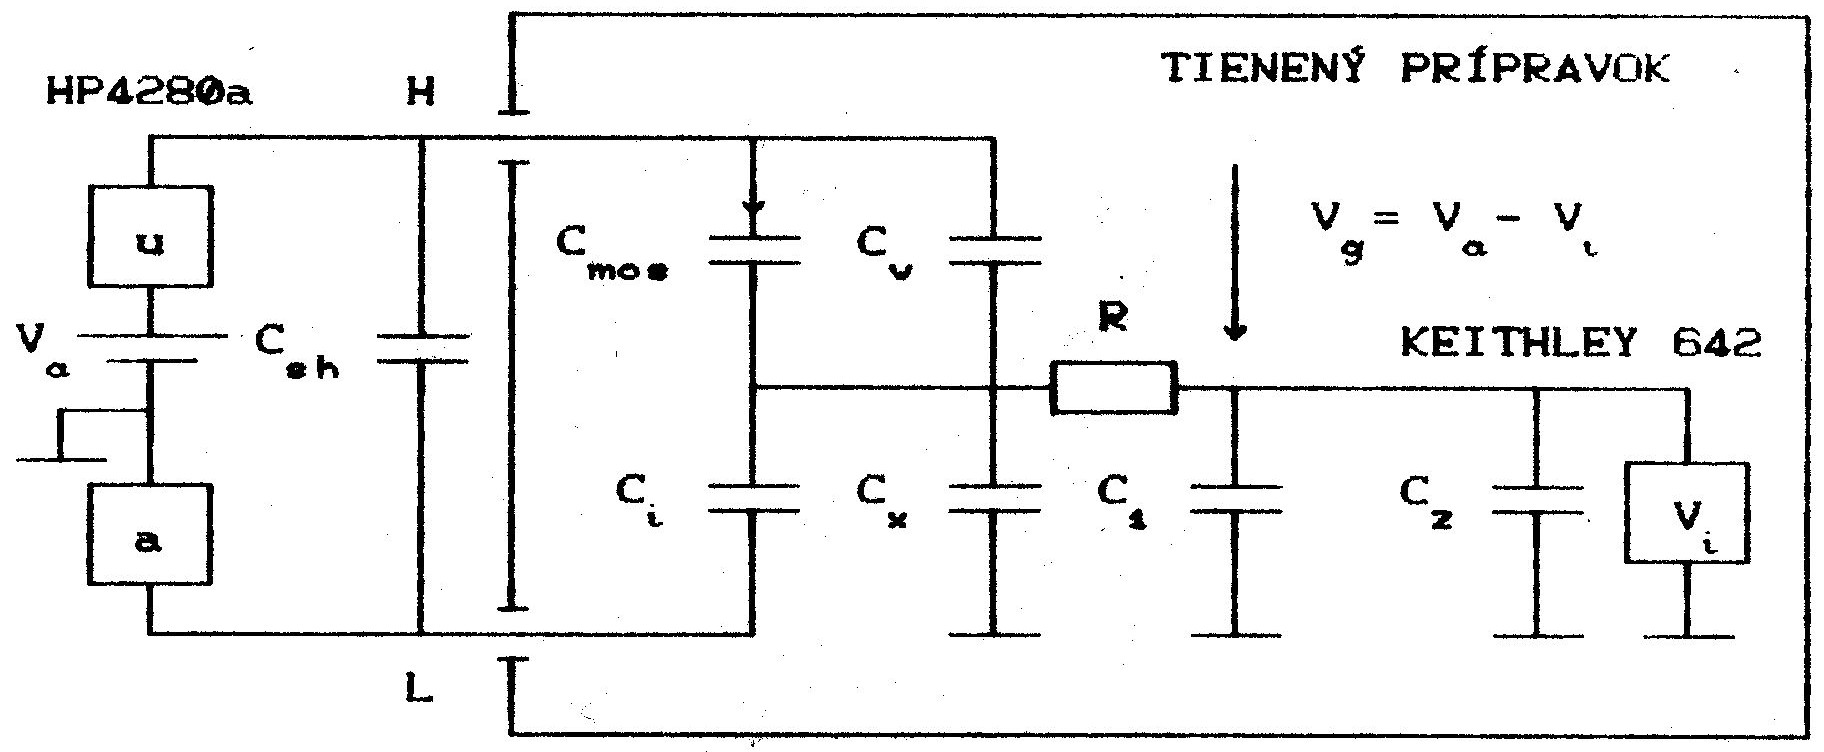
\includegraphics{Figures/fig-app-1.eps}
  \caption[Zapojenie Q-C metódy implementované na KME EF
    STU.]{Zapojenie Q-C metódy implementované na KME EF
    STU.}\label{fig:App.1}
\end{figure}

\par Na obrázku~\ref{fig:App.1} je znázornené detailné zapojenie
pracovného stolíka a meracích prístrojov Q-C metódy. V ľavej časti
obrázku je znázornený merací prístroj HP4280a, ktorý na našej schéme
pozostáva zo zdroja jednosmerného napätia $V_a$, ktorým je meraná
štruktúra privedená do požadovaného stavu, zdroja vysokofrekvenčného
signálu (označeného u) a ampérmetra (označeného a).  Kapacita $C_{sh}$
predstavuje parazitnú kapacitu prívodných vodičov, ktorú možno
eliminovať priamo pomocou meracieho prístroja HP4280a, a preto ju
ďalej nebudeme uvažovať. $C_{mos}$ je kapacita meranej štruktúry a
$C_i$ predstavuje napäťovo nezávislý kondenzátor. Kapacita $C_w$
znázorňuje parazitnú kapacitu medzi stolíkom, na ktorom sa nachádza
meraná štruktúra a zdvihnutým hrotom sondy. $C_x$ označuje parazitnú
kapacitu medzi spoločným bodom zapojenia kondenzátorov (ďalej len
spoločný bod) a zemou.  $C_1$ predstavuje parazitnú kapacitu
prívodného vodiča k voltmetru a $C_2$ označuje vstupnú kapacitu
voltmetra.  Uvedené kapacity $C_1$ a $C_2$ tvoria spolu s odporom R
dolnopriepustný filter, ktorý odizoluje voltmeter od
vysokofrekvenčného signálu, generovaného prístrojom HP4280a. Problémom
vysokofrekvenčného merania je skutočnosť, že ampérmeter prístroja
HP4280a nemeria zložku prúdu tečúcu zo spoločného bodu cez
kondenzátory $C_x$, $C_1$ a $C_2$ na zem. Uvedenú skutočnosť treba
zohľadniť pri vyhodnotení vysokofrekvenčného merania. Pre konečné
vyhodnotenie nameraných údajov je potrebné vyriešiť následovné úlohy:

\begin{itemize}
\item určenie kapacity $C_i$
\item určenie parazitnej kapacity $C_w$
\item určenie parazitnej kapacity $Cx$
\item určenie kapacity $C_{iLF}  = C_i  + C_1  + C_2$
\item korekcia meranej vysokofrekvenčnej kapacity $C_m$ vzhľadom na
  prúd tečúci cez $C_x + C_1 + C_2$ na zem.
\end{itemize}


\section{Určenie parazitnej kapacity $C_w$.}\label{sec:E.1}

Podrobný popis metodiky merania parazitnej kapacity $C_w$ je v dodatku
2.\ literatúry~\cite{App.2}. V našom experimente sme spomenutú
metodiku modifikovali spôsobom, ktorý viedol k väčšej
reprodukovateľnosti výsledkov. Tento postup popíšeme.

\begin{enumerate}

\item Pripojíme štruktúru MOS a pri $V_a = 0$ na okamih uzemníme
  spoločný bod, aby sme zaistili nulový vonkajší náboj na
  kondenzátoroch.

\item Napätím $V_a$ privedieme štruktúru MOS do akumulácie a odčítame
  hodnoty $V_a = V_{a0}$ a $V_i = V_{i0}$.

\item Privedieme štruktúru MOS vyšším napätím $V_a$ do akumulácie a
  odčítame hodnoty $V_a = V_{a1}$ a $V_i = V_{i1}$. Zo zákona zachovania
  náboja vyplýva
  \begin{equation}\label{eq:E.1}
    (C_{ox} + C_w)(V_{g1} - V_{g0}) = (C_{iLF} + C_x)(V_{i1} - V_{i0})
  \end{equation}

\item Nastavíme $V_a=0$, na okamih uzemníme spoločný bod a zdvihneme
  hrot sondy práve tak, aby sme prerušili kontakt.

\item Nastavíme $V_a \neq 0$ a odčítame hodnoty $V_a = V_{a2}$ a $V_i =  V_{i2}$.

\item Zvýšime napätie $V_a$ a odčítame hodnoty $V_a = V_{a3}$ a $V_i =  V_{i3}$. Zo zákona zachovania náboja vyplýva
  \begin{equation}\label{eq:E.2}
    C_w (V_{g3} - V_{g2}) = (C_{iLF} + C_x)(V_{i3} - V_{i2})
  \end{equation}

\item Porovnaním vzťahov~\ref{eq:E.1} a~\ref{eq:E.2} dostaneme výraz
  pre výpočet kapacity $C_w$, ktorú môžeme vyhodnotiť za predpokladu,
  že poznáme kapacitu oxidovej vrstvy štruktúry MOS\@.
  \begin{equation}\label{eq:E.3}
    C_w = C_{ox} \cfrac{1} {\cfrac {\cfrac{V_{g3}-V_{g2}}{V_{g1}-V_{g0}}} {\cfrac{V_{i3}-V_{i2}}{V_{i1}-V_{i0}}} -1}
  \end{equation}

\end{enumerate}


\section{Určenie parazitnej kapacity $C_x$.}\label{sec:E.2}

V dodatku 10.\ literatúry~\cite{App.4} sa nachádza popis priameho
merania parazitnej kapacity $C_x$. Avšak experimentálne výsledky
ukazujú, že toto meranie je zaťažené veľkou chybou a jeho
reprodukovateľnosť je malá. Preto sme zvolili v našom experimente
postup, ktorého princíp je načrtnutý v Dodatku
5.\ literatúry~\cite{App.4}. Ako možno vidieť v dodatku~\ref{sec:E.4},
vysokofrekvenčná kapacita štruktúry MOS $C_{mos}$ je funkciou
parazitnej kapacity $C_x$, ktorú chceme určiť. V akumulácii musí
platiť $C_{mos} = C_{ox}$, čo môžeme dosiahnuť vhodnou variáciou
hodnoty $C_x$. V našom vyhodnotení dát nameraných Q-C metódou sme na
variáciu hodnoty $C_x$ použili metódu delenia intervalov.


\section{Určenie kapacity $C_{iLF}$.}\label{sec:E.3}

V dodatku 10.\ literatúry~\cite{App.4} sa nachádza popis priameho
merania parazitnej kapacity $C_{iLF}$. Avšak podobne ako pri meraní
$C_x$ experimentálne výsledky ukazujú, že toto meranie je zaťažené
veľkou chybou. Preto sme zvolili postup, ktorý vychádza z podmienky,
že nízkofrekvenčná a vysokofrekvenčná kapacita štruktúry MOS musia mať
tú istú hodnotu v akumulácii. Určenie $C_{iLF}$ potom vychádza z
následujúceho vzťahu

\begin{equation}\label{eq:E.4}
  \frac{\delta}{\delta C_{iLF}} \sum\limits_{j} {\Big[C_{mos}^{LF}(j) - C_{mos}^{HF}(j)\Big]}^2 = 0
\end{equation}

,kde horeuvedenú sumáciu vykonávame pre body namerané v
akumulácii. Popis odvodenia vzťahu pre výpočet $C_{iLF}$ je v dodatku
4.\ literatúry~\cite{App.4} a tu uvedieme len jeho konečnú podobu.

\begin{equation}\label{eq:E.5}
  C_{iLF} = \frac{\sum\limits_{j}{\Big[C_{mos}^{HF}(j)+C_{w}\Big]}{\Big[\frac{dV_i}{dV_g}\Big]}_j}{\sum\limits_{j}{\Big[\frac{dV_i}{dV_g}\Big]}_j}
\end{equation}

Treba upozorniť, že uvedený postup má tú výhodu, že jeho použitie
zaručuje koincidenciu nízkofrekvenčnej a vysokofrekvenčnej kapacitnej
závislosti štruktúry MOS v akumulácii, čo predstavuje dobrý základ pre
výpočet pascí rozhrania z uvedených dvoch kapacitných závislostí.


\section{Korekcia vysokofrekvenčnej kapacity $C_m$.}\label{sec:E.4}

V dodatku 1.\ literatúry~\cite{App.2} je uvedená analýza zapojenia Q-C
metódy z pohľadu vysokofrekvenčného merania. Tu uvedieme jej hlavnú
myšlienku.

\begin{figure}[h!]\centering
  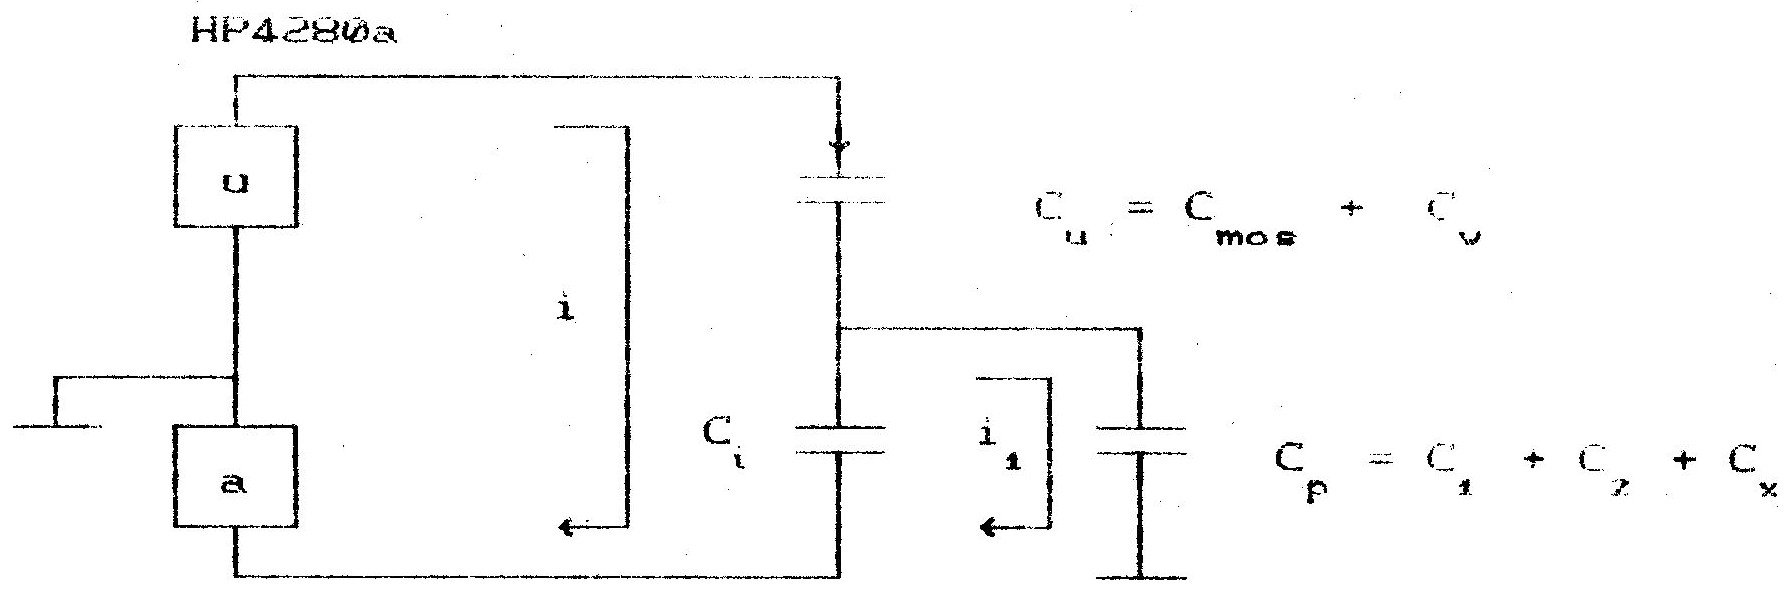
\includegraphics{Figures/fig-app-2.eps}
  \caption[Ekvivalentné zapojenie Q-C metódy pre vysokofrekvenčné
    meranie]{Ekvivalentné zapojenie Q-C metódy pre vysokofrekvenčné
    meranie.}\label{fig:App.2}
\end{figure}

Ako vidieť z obrázku~\ref{fig:App.2} ampérmeter prístroja HP4280a
nemeria prúd $i_1$ tečúci cez kondenzátor $C_p$. Kapacitu $C_m$, ktorú
pomocou tohoto prístroja nameriame, môžeme vyjadriť vzťahom

\begin{equation}\label{eq:E.6}
  C_m = \frac{C_{u} C_{iHF}} {C_{iHF}+C_{u}+C_{p}}
\end{equation}

V kapitole~\ref{sec:3.3} sú uvedené vzťahy pre výpočet
vyskofrekvenčnej kapacity štruktúry MOS\@.  Aby výsledky, získané zo
vzťahov~\ref{eq:3.3} neboli ovplyvnené uvedenou skutočnosťou, treba
urobiť následujúce korekcie (podľa dodatku 1.\ literatúry~\cite{App.4})

\begin{equation}\label{eq:E.7}
  C_{iHF}=C_{iHF}k, \qquad G_{m}=G_{m}k, \qquad C_{m}=C_{m}k
\end{equation}

,kde

\begin{equation}\label{eq:E.8}
  k = 1 + \frac{C_x}{C_{iHF}}
\end{equation}

% Appendix F

\chapter{Určenie povrchového potenciálu $\varphi_s$ z Q-C metódy.}\label{app:AppendixF}
\lhead{Appendix F. \emph{Určenie povrchového potenciálu $\varphi_s$ z Q-C metódy}}

Spôsob určenia povrchového potenciálu štruktúry MOS je popísany v
článku~\cite{App.3}. Tu uvedieme jeho hlavnú myšlienku.

Pre zmenu nábojov na sériovo-paralelnom zapojení kondenzátorov Q-C
metódy môžeme písať (pozri dodatok~\ref{app:AppendixE}).

\begin{equation}\label{eq:F.1}
  \Delta Q_x + \Delta Q_i = \Delta Q_w + \Delta Q_{mos}
\end{equation}

Ak vyjadríme zmenu náboja na napäťovo-nezávislých kondenzátoroch
pomocou ich kapacity a napätia, za predpokladu, že vychádzame zo stavu
kedy $V_i=0$ a $V_g=0$, môžeme písať

\begin{equation}\label{eq:F.2}
  \Delta Q_{mos} = (C_{iLF} + C_{x})V_{i} - C_{w}V_{g}
\end{equation}

Zmenu náboja na štruktúre MOS môžeme vyjadriť aj pomocou jej vlastných
parametrov

\begin{equation}\label{eq:F.3}
  \Delta Q_{mos} = C_{ox}(V_{g} - \varphi_{s} + \varphi_{s0})
\end{equation}

a kombináciou~\ref{eq:F.2} a~\ref{eq:F.3} môžeme písať výsledný vzťah

\begin{equation}\label{eq:F.4}
  \varphi_{s} = \varphi_{s0} - \frac{C_{iLF} + C_{x}}{C_{ox}}V_i + {\Big[1 + \frac{C_{w}}{C_{ox}}\Big]}V_{g}
\end{equation}

% Appendix G

\chapter{Určenie povrchového potenciálu $\varphi_{s0}$ pri nulovom napätí hradla.}\label{app:AppendixG}
\lhead{Appendix G. \emph{Určenie povrchového potenciálu $\varphi_{s0}$ pri nulovom napätí hradla}}

Vo vzťahu~\ref{eq:F.4} vystupuje výraz $\varphi_{s0}$, ktorý
predstavuje povrchový potenciál polovodiča štruktúry MOS v prípade, že
na štruktúru MOS nepôsobí žiadne vonkajšie napätie.  Tento potenciál
je spôsobený rozdielom výstupných prác kovu a polovodiča a nábojmi
nachadzájúcimi sa v izolante a na jeho rozhraní s polovodičom. Na
určenie tejto konštanty použijeme porovnanie nameranej a teoretickej
závislosti $\varphi_{s}$ od šírky OPN, ako je uvedené
v~\cite{App.3}. Šírku OPN pre experimentálnu závislosť
$\varphi_{s}(w)$ určíme zo vzťahu

\begin{equation}\label{eq:G.1}
  w = \epsilon \bigg[\frac{1}{C_{mos}^{HF}} - \frac{1}{C_{ox}}\bigg]
\end{equation}

Pre určenie teoretickej závislosti $\varphi_{s}(w)$ použijeme
aproximáciu popísanu v~\cite{App.5}

\begin{equation}\label{eq:G.2}
  \beta \varphi_{s} = \frac{1}{2} {\bigg[\frac{w}{L_{DE}}\bigg]}^2 + \frac{1}{N_{B}L_{DE}^{2}} \int_{0}^{w}x[N(x)-N_{B}]dx + 1
\end{equation}

kde $L_{DE}$ je extrinzická Debayova dĺžka, $N_{B}$ koncentrácia
substrátu a $N(x)$ priebeh koncentrácie dotujúcich prímesí v
podpovrchovej oblasti polovodiča. Na obrázku~\ref{fig:App.3} je
znázornený priebeh uvedených závislostí pre namerané dáta Q-C metódy z
obrázku~\ref{fig:3.4}. Hodnotu $\varphi_{s0}$ potom určíme z rozdielu
experimentálnej a teoretickej závislosti $\varphi_{s}(w)$ v hĺbke w,
ktorá zodpovedá stavu ochudobnenia štruktúry MOS\@. Ako je uvedené
v~\cite{App.3} aproximácia~\ref{eq:G.2} ignoruje voľné nosiče náboja,
z čoho vyplýva jej obmedzenie platnosti len pre stav ochudobnenia.
Uvedeným spôsobom možno vypočítať aj integračnú konštantu pri výpočte
závislosti $\varphi_{s}(V_{g})$ pomocou Berglundovho integrálu.

\begin{figure}[h!]\centering
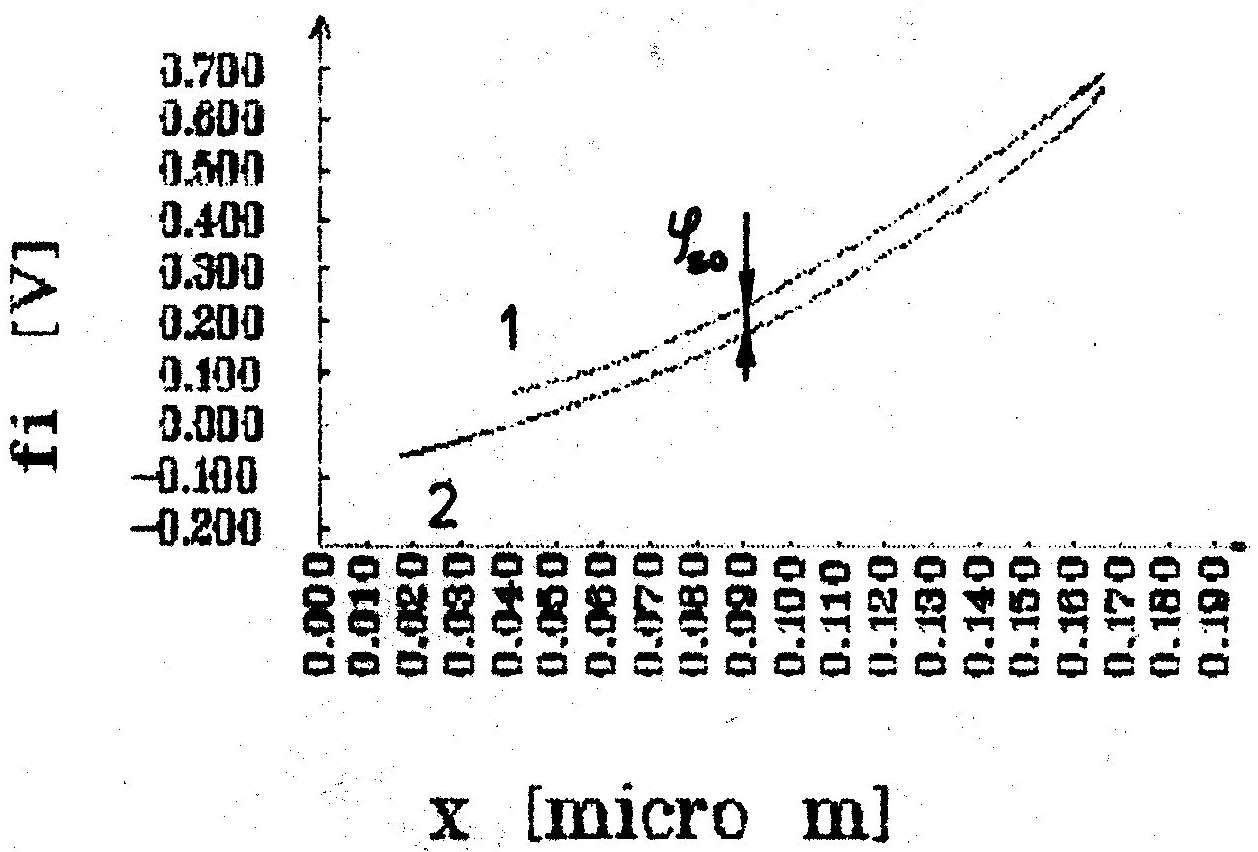
\includegraphics{Figures/fig-app-3.eps}
\caption[Priebeh povrchového potenciálu ako závislosti šírky OPN pre
  štruktúru MOS privedenú do stavu hlbokého ochudobnenia]{Priebeh
  povrchového potenciálu ako závislosti šírky OPN pre štruktúru MOS
  privedenú do stavu hlbokého ochudobnenia.  Krivka 1 predstavuje
  priebeh $\varphi(x)$ vypočítaný podľa vztahu~\ref{eq:G.2} a krivka 2
  znázorňuje závislosť určenú z experimentálnych dát pomocou
  vzťahu~\ref{eq:F.4}.}\label{fig:App.3}
\end{figure}
% OBR10.BIT

% Appendix H

\chapter{Programy zberu, spracovania a zobrazenia dát pre plošné rozloženie parametrov štruktúr MOS.}\label{app:AppendixH}
\lhead{Appendix H. \emph{Programy zberu, spracovania a zobrazenia dát}}

\begin{verbatim}
I. PROGRAMY ZBERU DAT.

  Vsetky programy zberu dat pouzivaju pre riadenie krokovacieho
  zariadenia programy:

* ZONDUP.EXE - zdvih stolika
* ZONDDN.EXE - spustenie stolika
* ZONDST.EXE - posuv stolika

  Informacie o pohybe krokovacieho zariadenia citaju zo suboru Z.XY

1. ZCT.EXE      - Hlavny program metody CCT
   segmenty:
   * ZCT1.EXE   - inicializacia zbernice IMS-2 a pristrojov
   * ZCT2.EXE   - meranie V(t) a ukladanie dV/dt do suboru
   * ZCT9.EXE   - uvedenie zbernice IMS-2 do povodneho stavu

2. ZHF.EXE      - Hlavny program rovnovaznej a nerovnovaznej HF CV metody
   segmenty:
   * ZHF1.EXE   - inicializacia zbernice IMS-2 a pristrojov
   * ZHF2.EXE   - meranie C(V )
   * ZHF3.EXE   - vyhladenie nameranych dat a ulozenie do suboru
   * ZHF9.EXE   - uvedenie zbernice IMS-2 do povodneho stavu

3. ZLF.EXE      - Hlavny program kvazistatickej CV metody
   segmenty:
   * ZLF1.EXE   - inicializacia zbernice IMS-2 a pristrojov
   * ZLF2.EXE   - meranie zavislosti C(V )
   * ZLF3.EXE   - vyhladenie nameranych dat, interpolacia a ulozenie do suboru
   * ZLF9.EXE   - uvedenie zbernice IMS-2 do povodneho stavu

4. ZOXHF.EXE    - Merania kapacity oxidu pomocou HF CV metody
   segmenty:
   * ZOXHF1.EXE - inicializacia zbernice IMS-2 a pristrojov
   * ZOXHF2.EXE - meranie kapacity oxidovej vrstvy a ukladanie do suboru
   * ZOXHF9.EXE - uvedenie zbernice IMS-2 do povodneho stavu

5. ZOXLF.EXE    - Merania kapacity oxidu pomocou kvazistatickej CV metody
   segmenty:
   * ZLF1.EXE   - inicializacia zbernice IMS-2 a pristrojov
   * ZOXLF2.EXE - meranie kapacity oxidovej vrstvy a ukladanie do suboru
   * ZLF9.EXE   - uvedenie zbernice IMS-2 do ppvodneho stavu


II. PROGRAMY SPRACOVANIA DAT.

6.    ZNX.EXE - vypocet koncentracneho profilu N(x)
7.    ZNB.EXE - vypocet koncentracie substratu N
8.    ZFV.EXE - vypocet povrchoveho potencialu ako funkcie 
                napbtia hradla f (V )
9.    ZDF.EXE - vypocet hustoty pasci rozhrania D
10.   ZTX.EXE - vypocet generacneho casu zivota minoritnych 
                nosicov naboja t (x)
11.  ZWOX.EXE - vypocet hrubky oxidu h
12.  ZYXI.EXE - vypocet integralnej hodnoty Y(x)
13.  ZYXM.EXE - vypocet strednej hodnoty, smerodajnej od-
                chylky a linearnej regresie
14.ZKORFF.EXE - vypocet korelacneho koeficientu medzi para-
                metrami zo suborov Subor1 <> Subor2
15.ZKORYX.EXE - vypocet korelacneho koeficientu zavislosti Y(x)


III. PROGRAMY GRAFICKEHO ZOBRAZENIA DAT.

16.   ZGF.EXE - zobrazenie zavislosti Y(x) s popisom osi
17. ZSURF.EXE - plosne zobrazenie rozlozenia parametrov a
                funkcnych zavislosti Y(x), pre rpzne x
18. ZVIEW.EXE - zobrazenie jednotlivych zavislosti Y(x)
19.ZVIEWD.EXE - zobrazenie jednotlivych zavislosti Y1(x) a Y2(x)


IV. POMOCNE PROGRAMY.

20.   BELL.EXE - alarm
21. ZASCII.EXE - konverzia binarneho formatu na ASCII
22.   ZERR.EXE - vypis pozicii na doske s chybne nameranymi datami
23. ZREPLC.EXE - vymena zaznamov v datovom subore
24. ZTRUNC.EXE - skratenie datoveho suboru
\end{verbatim}

% Appendix Bibliography
%\chapter{Literatúra k dodatkom} % Main appendix title
%\label{app:AppendixBibliography} % For referencing this appendix elsewhere, use \ref{AppendixA}
%\lhead{\emph{Literatúra k dodatkom}} % This is for the header on each page - perhaps a shortened title

\begin{thebibliography}{}

\bibitem[App.1]{App.1}
  \href {http://ieeexplore.ieee.org/xpl/login.jsp?tp=&arnumber=4236397&url=http\%3A\%2F\%2Fieeexplore.ieee.org\%2Fstamp\%2Fstamp.jsp\%3Ftp\%3D\%26arnumber\%3D4236397}
  {El- Sissi H., Cobbold R.S.C. : Electronic Letters 25 (1973) s.594.}
  
\bibitem[App.2]{App.2}
  \href {http://www.sciencedirect.com/science/article/pii/0038110184900698}
  {Nicollian E.H., Brews J.R. : Solid St. Electron. 27 (1984) s.953.}
  
\bibitem[App.3]{App.3}
  \href {http://www.sciencedirect.com/science/article/pii/0038110184900704}
  {Brews J.R., Nicollian E.H. : Solid St. Electron. 27 (1984) s.963.}
  
\bibitem[App.4]{App.4}
  \href {http://www.sciencedirect.com/science/article/pii/0038110184900716}
  {Boulin D.M., Brews J.R., Nicollian E.H. : Solid St. Electron. 27 (1984) s.977.}
  
\bibitem[App.5]{App.5}
  \href {http://www.sciencedirect.com/science/article/pii/0038110182901228}
  {Brews J.R. : Solid St. Electron. 25 (1982) s.375.}
  
\end{thebibliography}

\addtocontents{toc}{\vspace{2em}} % Add a gap in the Contents, for aesthetics

%----------------------------------------------------------------------------------------
%	INDEX
%----------------------------------------------------------------------------------------
\newpage
\lhead{\emph{Index}} % Change the page header to say "Index"
\addcontentsline{toc}{chapter}{Index}
\printindex
%----------------------------------------------------------------------------------------
%	BIBLIOGRAPHY
%----------------------------------------------------------------------------------------
% \newpage
% \lhead{\emph{Literatúra}}\backmatter% Change the page header to say "Bibliography"
% \bibliographystyle{unsrtnat}% Use the "unsrtnat" BibTeX style for formatting the Bibliography
% \bibname{Literatúra}
% \bibliography{Literatúra}\label{Bibliography} % The references (bibliography) information are stored in the file named "Bibliography.bib"

\end{document}  
